\chapter{Near Detector Executive Summary}
\label{ch:exsum-nd}


%%%%%%%%%%%%%%%%%%%%%%%%%%%%%%%%%%%%%%%%%%%%%%%%%%%%%%%%%%%%%%
\section{Brief Overview of the DUNE Near Detector}
\label{sec:exsum-nd-overview}

%The aim of the \dword{dune} experiment is to measure the oscillation probabilities for muon neutrino and muon antineutrinos to either remain the same flavor or oscillate to electron (anti)neutrinos. Measuring these probabilities as a function of the neutrino energy will allow the extraction of the mass ordering (MO) and the CP-violating phase \deltacp.  The near detector (ND) is an important tool for constraining the systematic uncertainties of the oscillation measurements. This is the main driver behind the design of the \dword{dune} \dword{nd}. 

\subsection{Need for the Near Detector}
\label{sec:BriefOverview-need}

The primary aim of the \dword{dune} experiment is to measure the oscillation probabilities for muon neutrino and muon antineutrinos to either remain the same flavor or oscillate to electron (anti)neutrinos. Measuring these probabilities as a function of the neutrino energy will allow the extraction of the mass ordering (MO) and the \dword{cp}-violating phase \deltacp.

The role of the \dword{nd} is to serve as the experiment's control. The \dword{nd} establishes the null hypothesis and constrains systematic errors. It measures the initial unoscillated \numu and \nue energy spectra: the convolution of flux, cross section, and detector response. To first order, a ``Far/Near'' ratio (or migration matrix), derived from the simulation, can predict the unoscillated energy spectrum at the \dword{fd} based on the \dword{nd} measurements.  The energy spectra at the \dword{fd} are then sensitive to the oscillation parameters, which can be extracted via a fit.

To achieve the precision needed for \dword{dune}, the experiment will have to operate beyond the first-order paradigm. With finite energy resolution and non-zero biases, the reconstructed energy spectrum is an unresolved convolution of cross section, flux, and energy resolution. The \dword{nd} must independently constrain each of those components.  The \dword{nd} must provide information that can be used to model well each component. It is the models of the detector, beam, and interactions that fill in holes and biases left by imperfect understanding and are used to estimate the size of many systematic effects.  In general, this requires that the \dword{nd} significantly outperform the \dword{fd}, which is limited by the need for a large, underground, mass. The \dword{nd} must have multiple methods for measuring neutrino fluxes as independently from cross section uncertainties as possible. With the necessity of relying on models, the \dword{nd} needs to measure neutrino interactions with much better detail than the \dword{fd}. This includes having a larger efficiency across the kinematically allowed phase space of all relevant reaction channels, superior identification of charged and neutral particles, better energy reconstruction, and better controls on experimental biases. The \dword{nd} must also have the ability to measure events in a similar way to the \dword{fd}, so that it can determine the ramifications of the more limited \dword{fd} performance, provide corrections, and take advantage of effects cancelling to some extent in the near to \dword{fd} extrapolation.

The conceptual design of the \dword{nd} is based on the collective experience of the many \dword{dune} collaborators who have had significant roles in the current generation of neutrino experiments (\dword{minos}, MiniBooNE, \dword{t2k}, \dword{nova}, \dword{minerva}, and the \dword{sbn} program).  These programs have provided (and will provide) a wealth of useful data and experience that has led to improved neutrino interaction models, powerful new analyses and reconstruction techniques, a deep appreciation of analysis pitfalls, and a better understanding of the error budget. 
These experiments, while similiar to \dword{dune}, were all either done at a lower precision, in a different energy range, or with very different detector technologies. While the existing and projected experience and data from those experiments provides a strong base for \dword{dune}, it is not sufficient to enable \dword{dune} to accomplish its physics goals without a highly performing \dword{nd}.  

The \dword{dune} \dword{nd} will also have a physics program of its own measuring cross sections, \dwords{nsi}, searching for sterile neutrinos, dark photons and other exotic particles. These are important aims that expand the physics impact of the \dword{nd} complex.  Also the cross section program is coupled to the oscillation measurement in so far as the cross sections and smearing functions used in the oscillation analysis will come from a \dword{mc} tuned with standalone cross section measurements.

\subsection{Overview of the Near Detector}
\label{sec:BriefOverview}

The \dword{dune} \dword{nd} is formed from four components that serve important individual and overlapping functions with regard to the mission of the \dword{nd}.  Because these components have standalone features, the \dword{dune} \dword{nd} is often discussed as a suite or complex of detectors and capabilities.  The power in the \dword{dune} \dword{nd} concept lies in the collective set of capabilities.  It is not unreasonable to think of the component detectors in the \dword{dune} \dword{nd} as being somewhat analogous to subsystems in a collider experiment, the difference being that, with one important exception, individual events are contained within the subsystems.  
The \dword{dune} \dword{nd} is shown in the \dword{dune} \dword{nd} hall in Figure~\ref{fig:NDHallconfigs}.  Table~\ref{NDsumm} provides a high-level overview of the four components of the \dword{dune} \dword{nd}.  

\begin{dunefigure}[DUNE near detector hall.]{fig:NDHallconfigs}
{\dword{dune} \dword{nd} hall shown with component detectors all in the on-axis configuration (left) and with the \dword{lartpc} and \dword{mpd} in an off-axis configuration (right). The \dword{3dsts} is shown in position on the beam axis. The beam axis is shown.  The beam enters the hall at the bottom of the drawings moving from right to left.}
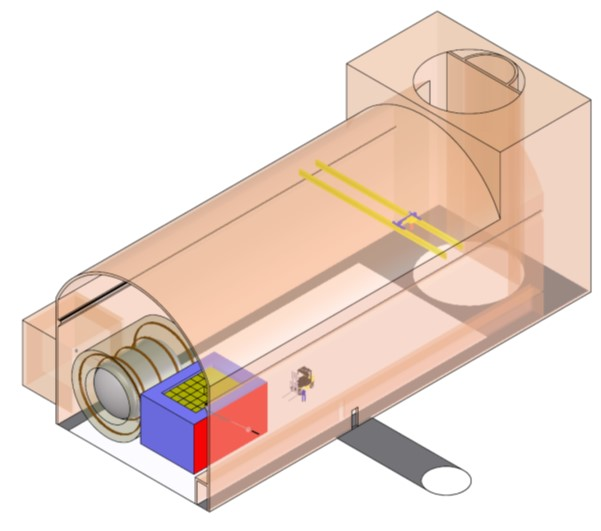
\includegraphics[width=0.49\textwidth]{graphics/NDHall_onaxis.jpg}
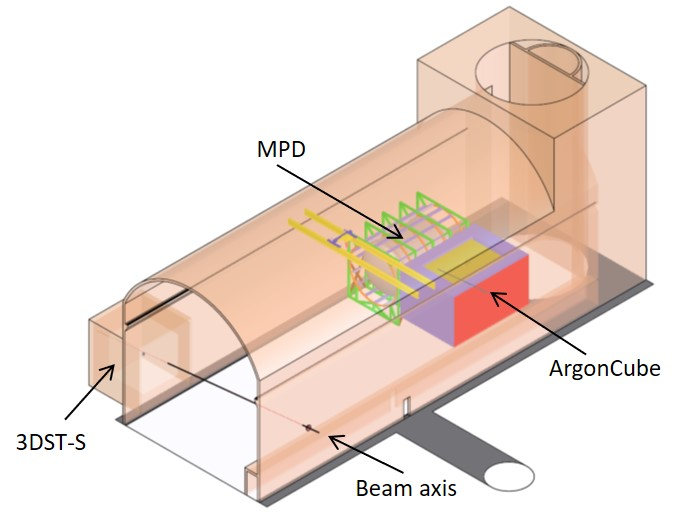
\includegraphics[width=0.49\textwidth]{graphics/NDHall_offaxis.jpg}
\end{dunefigure}

\begin{dunetable}[Components of the \dword{dune} \dword{nd}]{llll}{NDsumm}{This table gives a high-level breakdown of the four major components of the \dword{dune} \dword{nd} along with function and primary physics goals.}
Component & Essential Characteristics & Primary function & Select physics aims \\ \toprowrule
\dword{arcube} & Mass  & Flux determination & $\numu$($\overline{\nu}_{\mu}$) \dword{cc} \\
          & Target nucleus Ar &  \dword{fd} detector response   & $\nu$-e$^{-}$ scattering   \\
          &  Technology \dword{fd}-like    &            &  $\nue +$$\overline{\nu}_{e}$ \dword{cc}  \\
          &  &  &  Interaction model \\\colhline
Multipurpose detector & Magnetic field & p analyze \dword{lar} $\mu$ & $\numu$($\overline{\nu}_{\mu}$) \dword{cc} \\
  &  Target nucleus Ar & Low p charged particles & Interaction model \\
  & Low density & & $\nue$ \dword{cc}, $\overline{\nu}_{e}$ \dword{cc} \\  \colhline
\dword{duneprism} & \dword{lar}$+$\dword{mpd} move off-axis & Change flux spectrum &  Deconvolute xsec*flux \\ 
 & & & Detector reponse \\
 & & & Minimize ND-FD flux\\ 
 & & & {\   }differences \\
 & & & ID mismodeling \\ \colhline
\dword{3dsts} & On-axis & Beam flux monitor &  On-axis flux stability \\ 
  & Mass & Neutrons & Interaction model \\ 
& Magnetic field &  & A dependence \\
    & CH target & & $\nu$-e$^{-}$ scattering \\ \colhline
\end{dunetable}



%The ambitious and varied goals for the \dword{dune} oscillation physics program have led to a concept of a complementary suite of powerful detectors and capabilities.  Each element in the concept aims to address part of the mission in an optimal and complementary fashion relative to the other elements.  To the extent there is some overlap in functionality, multiple measurements and approaches will provide the confidence and sensitivity to unexpected surprises necessary to minimize the overall systematic errors. 

The core part of the \dword{dune} \dword{nd} is a \dword{lartpc} called \dword{arcube}.  The particular implementation of the \dword{lartpc} technology in this detector is described in Section~\ref{sec:exsum-nd-lartpc} below.  
This detector has the same target nucleus and shares some aspects of form and functionality with the \dword{fd}, where the differences are necessitated by the expected intensity of the beam at the \dword{nd}.  This similarity in target nucleus and, to some extent, technology reduces sensitivity to nuclear effects and detector-driven systematic errors in the extraction of the oscillation signal at the  \dword{fd}.  The \dword{lartpc} is large enough to provide high statistics and a sufficient volume to provide good hadron containment.  The tracking and energy resolution, combined with the mass of the \dword{lartpc}, will allow for the measurement of the flux in the beam using several techniques, including the rare process of $\nu$-e$^{-}$ scattering.

The \dword{lartpc} begins to lose acceptance for muons above $\sim$0.7 GeV/c due to lack of containment.  Because the muon momentum is a critical component of the neutrino energy determination, a magnetic spectrometer is needed downstream of the \dword{lartpc} to measure the charge sign and momentum of these muons.  In the \dword{dune} \dword{nd} concept, this function is accomplished by the multipurpose detector (\dword{mpd}) which consists of a high-pressure gaseous argon \dword{tpc} (\dword{hpgtpc}) surrounded by an \dword{ecal} in a \SI{0.5}{T} magnetic field. The \dword{hpgtpc} provides a lower density medium with excellent tracking resolution for the muons from the \dword{lartpc}.  In addition, with this choice of technology for the tracker, neutrinos interacting on the argon in the gas \dword{tpc} constitute a sample of $\nu$-Ar events that can be studied with a very low charged particle tracking threshold and excellent resolution and systematic errors that differ from the liquid detector. These events are expected to be valuable for studying the charged particle activity near the interaction vertex since this detector can access lower momenta protons than the \dword{lar} detector and has better particle identification of charged $\pi$.  In addition, the lack of secondary interactions in these samples will be helpful for identifying the particles produced in the primary interaction and modeling secondary interactions in denser detectors, which are known to be important \cite{Friedland:2018vry}.
The high pressure increases the statistics for these studies.  
%These events are expected to be very valuable for developing, tuning, and gaining confidence in the neutrino interaction model used for the extraction of oscillation parameters.  
The \dword{mpd} is  discussed further in Section~\ref{sec:exsum-nd-mpt}.


The \dword{lartpc} and \dword{mpd} can move to take data in positions off the beam axis.  This capability is referred to as \dword{duneprism}. As the detectors move off-axis, the incident neutrino flux spectrum changes, with the mean energy dropping and the spectrum becoming somewhat monochromatic.  Though the neutrino interaction rate drops off-axis, the intensity of the beam and the size of \dword{arcube}  combine to yield ample statistics even in the off-axis positions.
Data taken at different off-axis angles allows for the deconvolution of the neutrino flux and interaction cross section and the mapping of the reconstructed versus true energy response of the detector.  This latter mapping is applicable at the \dword{fd} up to the level to which the near and far \dword{lar} detectors are similar.  Stated a different way, it is possible to use information from a linear combination of the different fluxes to create a data sample at the \dword{nd} with an effective neutrino energy distribution that is close to that of the oscillated spectrum at the \dword{fd}.  This data-driven technique will reduce systematic effects coming from differences in the energy spectra of the oscillated signal events in the \dword{fd} and the \dword{nd} samples used to constrain the interaction model. Finally, the off-axis degree of freedom provides a sensitivity to some forms of mis-modeling in the beam and/or interaction models. \dword{duneprism} is discussed further in Section~\ref{sec:exsum-nd-DP}.

The final component of the \dword{dune} \dword{nd} suite is the \threed projection scintillator tracker spectrometer (\dword{3dsts}),  the core part of which is the \dword{3dst}.  The \dword{3dst} is a plastic scintillator detector made of \SI{1}{cm} cubes that are read out along each of three orthogonal dimensions.  The design eliminates the typical planar-strip geometry common to detectors using scintillator, leading to improved acceptance at large angles relative to the beam direction.  The \dword{3dst} is situated along the beam axis inside an envelope of high resolution, normal pressure \dwords{tpc} and an \dword{ecal}.  The entire structure is enclosed in a magnet. This device importantly serves as a consistent, on-axis neutrino spectrum monitor.   It also provides an excellent on-axis, neutrino flux determination using many of the methods discussed in Section~\ref{ssec:flux}, even when the \dword{lartpc} has moved to an off-axis position.  The neutrino flux determined using this detector, with  differing detector and interaction systematic errors as compared to the \dword{lartpc}, can be used as an important point of comparison and systematic crosscheck for the flux as determined by the \dword{lartpc}.
In addition, the \dword{3dst} has very fast timing and the ability to isolate small energy depositions from neutrons in three dimensions.  This provides the capability to  incorporate neutrons in the event reconstruction using energy determination via time-of-flight with a high efficiency.  
The fact that the target nucleus is carbon rather than argon is a complicating factor in using the neutrino interaction data in the \dword{3dst} to constrain the interaction model on argon.  
On the other hand, the A dependence offers an extra degree of freedom that is important for developing models of nuclear effects and building confidence in the interaction model and the size of numerous systematic errors.  Also, recent electron scattering results on C, Ti, and Ar targets are described very well by the SuSAv2-MEC superscaling framework and this is expected to be applicable to neutrinos~\cite{Barbaro:2019vsr}.  The \dword{3dsts} component of the \dword{nd} is discussed more in Section~\ref{sec:exsum-nd-mpt-3dst}.


The rest of the \dword{nd} executive summary discusses the \dword{nd} mission in general and provides significantly more detail on the characteristics and capabilities of the four components of the \dword{nd}, and how the data from the different detectors feed into the overall \dword{dune} physics strategy. 


\section{Role of the Near Detector in the DUNE Oscillation Program}
\label{sec:exsum-nd-role}

Oscillation experiments need to accomplish three main tasks. First, they must identify the flavor of interacting neutrinos in \dword{cc} events, or identify the events as \dword{nc} interactions. Second, they need to measure the energy of the neutrinos since oscillations occur as a function of baseline length over neutrino energy, \dword{l/e}. Third, they need to infer the flux of the neutrinos at the \dword{fd} from the measured interaction rate, using knowledge of neutrino cross sections. The inferred flux is then compared with a prediction based on a beam simulation usually constrained by similar measurements conducted with a  \dword{nd}. The difference in the predicted and measured fluxes is sensitive to the oscillation parameters.

In a real experiment %there is 
a host of complicating effects %that 
muddy this simple picture. They come from two main sources. First, the identification efficiency is not \SI{100}{\%} and there is 
some background (for example, \dword{nc} events with a $\pi^0$ are a background to \nue \dword{cc} interactions). Both the efficiency and the background are imperfectly known. Generally, it is helpful to have a  \dword{nd} that is as similar as feasible to the  \dword{fd} because a bias in the efficiency as a function of energy will cancel between the two detectors. Since the background level tends to be similar between the two detectors, it is helpful if the \dword{nd} is more capable than the \dword{fd} at characterizing backgrounds, either due to its technology, or by leveraging the much larger statistics and freedom to take data in alternative modes (for example running without horns on provides a sample to constrain \dword{nc} backgrounds).

The second major source of complication occurs because the \dword{fd} (and the similar \dword{nd}) has to be made of heavy nuclei rather than hydrogen. Neutrino interactions can be idealized as a three stage process: (1) a neutrino impinges on a nucleus with nucleons in some initial state configuration, (2) scattering occurs with one of the nucleons, perhaps creating mesons, and (3) the hadrons reinteract with the remnant nucleus on their way out (so called \dwords{fsi}). The presence of the nucleus impacts all three stages in ways that ultimately drives the design of the  \dword{nd} complex. To better understand this it is useful to consider what would happen if the detectors were made of hydrogen.

%*** thoughts in this section were influenced by the S.C. group (R. Petti, S. Mishra) ***

If the detectors were made of hydrogen the initial state would just be a proton at rest and there would be no \dword{fsi}. The scattering consists of a variety of processes. The simplest is \dword{qe} scattering: $\bar{\nu}_\ell p \to \ell^+ n$. The detector sees a lepton (which establishes the flavor of the neutrino), no mesons, and perhaps a neutron interaction away from the lepton's vertex. Because there are no mesons the kinematics is that of two body scattering and the neutrino energy can be reconstructed from the the lepton's angle (with respect to the $\nu$ beam) and energy. This is independent of whether the neutron is observed.

For $\nu_\ell$ interactions on hydrogen there is no QE process. The simplest scattering channel is single pion production $\nu_\ell p \to \ell^- \pi^{(+,0)} (n,p)$. In that case the neutrino energy may be reconstructed from the energy of the muon and pion, and their angles with respect to the beam\footnote{The nucleon does not need to be observed. This is a consequence of having four energy-momentum conservation constraints, which allows $E_\nu$ and $\vec{p}_N$ to be computed.}. In both cases, the neutrino energy can be measured without bias so long as the detector itself measures lepton and meson momenta and angles without bias.  The neutrino energy in complicated scattering channels, such as ones with multiple pions or heavy baryons can be measured in a similar way (at least in principle).

A key simplifying feature offered by a hypothetical hydrogen detector is simply that there are enough constraints to measure the neutrino energy and also to neglect energy carried off by the single nucleon (especially a neutron escaping the detector). Additionally, the cross sections for different scattering channels (particularly the simpler ones) can be expressed in terms of leptonic and hadronic currents. The leptonic current is well understood. The structural elements of the hadronic current are known on general theoretical grounds. The current is often represented by form factors that are constrained by electron scattering experiments, beta decay, and measurements that the detector can make itself (or take from other experiments). 

%This is not the case for scattering off of a heavy nucleus.

% IS
% multiple nucleons
% FSI
% shorter path lengths, absorption of pi-, reinteractions knocking out neutrons

The situation is significantly more complicated in a detector with heavy nuclei. The nucleons in the initial state of the nucleus are mutually interacting and in motion. Their momentum distribution that is usually modeled as a Fermi gas with a cutoff momentum $k_F \approx 
\SI{250}{MeV/c}$\cite{Smith:1972xh}. This motion ruins the the key constraint available in hydrogen due to the target being at rest. The Fermi gas also suppresses scattering at lower momentum transfers because the nucleon in the final state has a momentum that is excluded by the Pauli principle.  Moreover, there are nucleons with momenta larger than $k_F$ due to \dword{src} \cite{Bodek:2014jxa}. Scattering on a nucleon with $p>k_F$ implies that there is a spectator nucleon recoiling against the target with a significant momentum. \dword{src} have been the subject of much investigation and are not fully understood or fully implemented in neutrino event generators.

Additionally, there is a second multibody effect. For the few-GeV neutrinos of interest to \dword{dune}, the typical momentum transfer corresponds to a probe that has a wavelength on par with the size of a nucleon. In this case the scattering can occur on two targets in the nucleus which may not be closely correlated (\dword{2p2h} scattering). Experiments can easily confuse this process for \dword{qe} scattering since there are no mesons and one or both of the two nucleons may have low energy, evading detection. The presence of two nucleons in the initial and final state again ruins the kinematic constraints available in hydrogen. It is now known that \dword{2p2h} scattering is a significant part of the total scattering cross section at \dword{dune} energies \cite{Ruterbories:2018gub}. The \dword{2p2h} cross section is difficult to compute because it cannot be expressed as the sum over cross sections on individual nucleons. The dependence on atomic number and the fine details of the interaction (e.g., the final energies of the two particles) are also currently unknown. Finally, it is widely expected that there are components of \dword{2p2h} and \dword{src} scattering that result in meson production. Event generators do not currently include those processes.

%It is possible to probe 2p2h and \dword{src} interactions with a near detector that has good reconstruction 

Neutrino scattering on nuclei is also subject to \dwords{fsi}. \dword{fsi} collectively refers to the process by which unbound nucleons and mesons produced by the neutrino interaction traverse the remnant nucleus. The hadrons reinteract with a variety of consequences: additional nucleons can be liberated; ``thermal'' energy can be imparted to the nucleus; pions can be created and absorbed; and pions and nucleons can undergo charge exchange scattering (e.g., $\pi^- p \to \pi^0 n$).  Event generators include phenomenological models for \dword{fsi}, anchoring to hadron nucleus scattering data.

%Generally FSI effects degrade particle energies, producing lower and lower energy particles.

% shorter path lengths, absorption of pi-, reinteractions knocking out neutrons

The heavy nuclei in a detector also act as targets for the particles that have escaped the struck nucleus. Generally speaking, the denser the detector and the more crudely it samples deposited energy, the more difficult it is to observe low-energy particles. Negatively and positively charged pions leave a different signature in a detector since the former are readily absorbed while the latter are likely to decay.  Neutrons can be produced from the struck nucleus, but also from follow on interactions of the neutrino's reaction products with other nuclei. The energy carried away by neutrons is challenging to detect and can bias the reconstructed neutrino energy. 



\subsection{Constraining the Flux}
\label{ssec:flux}

The \dword{dune}  \dword{fd} will not measure the neutrino oscillation probability directly. Instead, it will measure the neutrino interaction rate for different neutrino flavors as a function of the reconstructed neutrino energy. It is useful to formalize the measurements that are performed in the near and  far \dwords{detmodule} in the following equations:
\begin{align}
\label{eq:fdrate}
\frac{dN^{FD}_{x}}{dE_{rec}}(E_{rec}) & = 
\int \Phi^{FD}_{\numu}(E_\nu)P_{\numu\rightarrow x}(E_\nu)\sigma^{Ar}_x(E_\nu)T^{FD,Ar}_x(E_\nu,E_{rec})dE_\nu\\
\frac{dN^{ND}_{x}}{dE_{rec}}(E_{rec}) & = 
\int \Phi^{ND}_{x}(E_\nu)\sigma^m_x(E_\nu)T^{d,m}_x(E_\nu,E_{rec})dE_\nu\\
\mbox{with\hspace{2cm} } x & = \nue , \numu \nonumber \\
d & = \mbox{detector index} \nonumber \\
m & = \mbox{interaction target/material, (e.g., H, C, or Ar)} \nonumber \\
E_\nu & = \mbox{true neutrino energy} \nonumber \\
E_{rec} & = \mbox{reconstructed neutrino energy} \nonumber \\
T^{d,m}_x(E_\nu,E_{rec}) & = \mbox{true to reconstruction transfer function} \nonumber \\
\sigma^m_x(E_\nu) & = \mbox{neutrino interaction cross section} \nonumber \\
\Phi^{d}_x(E_\mu) & = \mbox{un-oscillated neutrino flux} \nonumber \\
\frac{dN^{d}_{x}}{dE_{rec}}(E_{rec}) & = \mbox{measured differential event rate per target (nucleus/electron)} \nonumber 
\end{align}
There are equivalent formulae for antineutrinos. For simplicity, the instrumental backgrounds (wrongly selected events) and the intrinsic beam contaminations (\nue interactions in case of the appearance measurement) have been ignored. But an important function of the  \dword{nd} is also to quantify and characterize those backgrounds.

It is not possible to constrain the \dword{fd} neutrino flux directly, but the near-to-far flux ratio is believed to be tightly constrained by existing hadron production data and the beamline optics. As such Equation~\ref{eq:fdrate} can be rewritten as 
\begin{align*}
\frac{dN^{FD}_{x}}{dE_{rec}}(E_{rec}) & = 
\int \Phi^{ND}_{\numu}(E_\nu)R(E_\nu)P_{\numu\rightarrow x}(E_\nu)\sigma^{Ar}_x(E_\nu)T^{d,Ar}_x(E_\nu,E_{rec})dE_\nu\\
& \mbox{with } R(E_\nu) = \frac{\Phi^{FD}_{\numu}(E_\nu)}{\Phi^{ND}_{\numu}(E_\nu)} \mbox{ taken from the beam simulation} \nonumber
\end{align*}

It is not possible to measure only a near-to-far event ratio and extract the oscillation probability since many effects do not cancel trivially.  This is due to the non-diagonal true-to-reconstruction matrix, which not only depends on the underlying differential cross section, but also on the detector used to measure a specific reaction.
\begin{align*}
\frac{dN^{FD}_{x}}{dE_{rec}}(E_{rec})/{\frac{dN^{ND}_{\numu}}{dE_{rec}}(E_{rec})} & \neq  R(E_\nu)P_{\numu\rightarrow x}(E_\nu)\frac{\sigma^{Ar}_x(E_\nu)}{\sigma^{m}_{\numu}(E_\nu)}
\end{align*}
It is therefore important that the \dword{dune} \dword{nd} suite constrain as many components as possible.


While the near-to-far flux ratio is tightly constrained to the level of \SIrange{1}{2}{\%}, the same is not true for the absolute flux itself. \dword{t2k}, using hadron production data obtained from a replica target, can constrain the absolute flux at the  \dword{nd} to \SIrange{5}{6}{\%} in the peak region and to around 10\% in most of its energy range. The NuMI beam has been constrained to 8\% using a suite of thin target hadron production data. The better the \dword{nd} flux is known, the easier it is to constrain modeling uncertainties by measuring flux-integrated cross sections. Predicting the event rate at the  \dword{fd} to a few percent will require additional constraints to be placed with the  \dwords{nd} or substantial improvements in our understanding of the hadron production and focusing uncertainties. 

%There are 
Several handles to constrain the flux %, which 
are addressed below. Briefly they offer the following constraints:

\begin{itemize}
    \item The overall flux normalization and spectrum can be constrained by measuring neutrinos scattering off of atomic electrons.
    \item The energy dependence (``shape'') of the \numu and \anumu %\numubar
     flux can be constrained using the ``Low-$\nu$'' scattering process.
    \item The flux ratio $\anumu/\numu$ can be constrained using charged current coherent neutrino scattering.
    \item The $\nue/\numu$ flux ratio in the energy region that standard oscillation occurs in is well constrained by the beam simulation. The experiment can also measure the $\nue/\numu$ interaction ratio and constrain the flux ratio using cross section universality.
\end{itemize}


% event rates table
% GArTPC numbers from HPTPC report doc-6652
% numubar CC coherent is 12% of numu CC coherent according to doc-273
% (this is numubar in numu beam mode)
\begin{dunetable}[Event rates for flux constraining processes]{llll}{fluxrates}{Event rates for processes that can be used to constrain the neutrino flux. The rates are given per year for a \SI{1}{ton} (FV) \dword{hpgtpc}, a \SI{25}{ton} (fV) \dword{lartpc} \cite{bib:docdb6652}, and a \SI{9}{ton} (fV) \dword{3dst}. The flux for the \dword{hpgtpc} and \dword{lartpc} is from the simulated ``2017 engineered'' \dword{lbnf} beam with a primary momentum of \SI{120}{GeV/c} and \SI{1.1e21}{POT/year}. The flux for the \dword{3dst} is the \SI{80}{GeV}, three-horn, optimized beam with \SI{1.46e21}{POT/year}.  The detectors are assumed to be on-axis.}
Event class & \dword{hpgtpc} & \dword{lartpc} & \dword{3dst} \\ \toprowrule
\numu + $e^-$ elastic ($E_e>\SI{500}{MeV}$) & \num{1.3e2} & \num{3.3e3} & \num{1.1e3} \\ \colhline
\numu low-$\nu$ ($\nu<\SI{250}{MeV})$ & \num{2.1e5} & \num{5.3e6} & \num{1.48e6} \\ \colhline
\numu \dword{cc} coherent & \num{8.8e3} & \num{2.2e5} &  \\ \colhline
\anumu \dword{cc} coherent & \num{8.4e2} & \num{2.1e4} &  \\ \colhline
\end{dunetable}
 


\subsubsection{Neutrino-Electron Elastic Scattering}
\label{ssec:fluxintro-e-nu-scatt}



Neutrino-electron scattering ($\nu \ e \rightarrow \nu \ e$) is a pure electroweak process with calculable cross section at tree level. The final state consists of a single electron, subject to the kinematic limit 

\begin{equation}
1 - \cos \theta = \frac{m_{e}(1-y)}{E_{e}},
\end{equation}

where $\theta$ is the angle between the electron and incoming neutrino, $E_{e}$ and $m_{e}$ are the electron mass and total energy, respectively, and $y = T_{e}/E_{\nu}$ is the fraction of the neutrino energy transferred to the electron. For \dword{dune} energies, $E_{e} \gg m_{e}$, and the angle $\theta$ is very small, such that $E_{e}\theta^{2} < 2m_{e}$. 

The overall flux normalization can be determined by counting $\nu \ e \rightarrow \nu \ e$ events. Events can be identified by searching for a single electromagnetic shower with no other visible particles. Backgrounds from $\nu_{e}$ \dword{cc} scattering can be rejected by looking for large energy deposits near the interaction vertex, which are evidence of nuclear breakup. Photon-induced showers from neutral-current $\pi^{0}$ events can be distinguished from electrons by the energy profile at the start of the track. The dominant background is expected to be $\nu_{e}$ \dword{cc} scattering at very low $Q^{2}$, where final-state hadrons are below threshold, and $E_{e}\theta^{2}$ happens to be small. The background rate can be constrained with a control sample at higher $E_{e}\theta^{2}$, but the shape extrapolation to $E_{e}\theta^{2} \rightarrow 0$ is uncertain at the \SIrange{10}{20}{\%} level.

For the \dword{dune} flux, approximately \num{100} events per year per ton of fiducial mass are expected with electron energy above \SI{0.5}{GeV}. For a \dword{lartpc} mass of 25 tons, this corresponds to \num{3300} events per year. The statistical uncertainty on the flux normalization from this technique is expected to be $\sim$1\%. \dword{minerva} has achieved a systematic uncertainty just under 2\% and it seems plausible that \dune could do at least as well\cite{bib:minervanue}. The \dword{3dst} can also do this measurement with significant statistics and with detector and reconstruction systematics largely uncorrelated with \dword{arcube}.  The signal is independent of A and the background is small; so, it seems plausible the samples can be combined to good effect.


\subsubsection{The Low-$\nu$ Method}
\label{ssec:intro-low-nu}
The inclusive cross section for \dword{cc} scattering $(\nu_l+N\rightarrow l^-+X)$ does not depend on the neutrino energy in the limit where the energy transfered to the nucleus $\nu = E_\nu-E_{l} $ is zero~\cite{bib:original_lownu}.  In that limit, the event rate is proportional to the flux, and by measuring the rate as a function of energy, one can get the flux ``shape.'' This measurement has been used in previous experiments and has the potential to provide a constraint in \dune with a statistical uncertainty $<1\%$.

In practice, one cannot measure the rate at $\nu=0$. Instead it is necessary to restrict $\nu$ to be less than a few \SI{100}{MeV}.  This introduces a relatively small $E_\nu$ dependence into the cross section that must be accounted for to obtain the flux shape. Thus the  measurement technique depends on the cross section model but the uncertainty is manageable~\cite{bib:bodek_lownu}. This is particularly true if low-energy protons and neutrons produced in the neutrino interaction can be detected. 

\subsubsection{Coherent Neutrino-Nucleus Scattering}
The interactions $\nu_l + A \rightarrow l^- + \pi^+ + A$ and 
%$\anu_l + N   & \rightarrow l^+ + \pi^- + N$ 
occur with very low three momentum transfer to the target nucleus (A).  As such, the interactions proceed coherently with the entire nucleus, and do not suffer from nuclear effects (though background channels certainly do). These coherent interactions are most useful as a constraint on the $\anumu/\numu$ flux ratio. Identifying with high efficiency and purity requires a detector with excellent momentum and angular resolution.

\subsubsection{Beam \nue Content}
\label{ssec:beam-nue}
Electron neutrinos in a wideband beam come from two primary sources: kaon decays and muon decays. These ``beam'' \nue are an irreducible background in $\numu \to \nue$ oscillation searches. As such, the \dword{lbnf} beam was optimized to make the \nue flux as small as possible while maximizing the \numu flux. In the energy range relevant for oscillations (\SI{0.5}{GeV} - \SI{4.0}{GeV}) the predicted $\nue/\numu$ ratio varies between 0.5\% and 1.2\% as a function of energy. The beam \nue flux in the same energy range is strongly correlated with the \numu flux due to the decay chain $\pi^+\to\mu^+\numu$ followed by $\mu^+ \to \anumu{} e^+ \nue $ (and likewise for \anue). As a result, the \dword{lbnf}  beam simulation predicts that the uncertainty on the $\nue/\numu$ ratio varies from \SIrange{2.0}{4.5}{\%}. At the  \dword{fd}, in a 3.5 year run, the statistical uncertainty on the beam \nue component is expected to be 7\% for the $\nu$ mode beam and 10\% for the $\bar{\nu}$ mode beam. The systematic uncertainty on the beam \nue flux is therefore subdominant, but not negligible.  



\subsection{Lessons from Current Experiments}
\label{ssec:exsum-nd-overview-lessons}

Neutrino beams are notoriously difficult to model at the precision and accuracy required for modern accelerator-based experiments.  Recent long-baseline experiments make use of a  \dword{nd} placed close to the beam source, where oscillations are not yet a significant effect.  The beam model, the neutrino interaction model, and perhaps the detector response model are tuned, or calibrated, by the data recorded in the  \dword{nd}. The tuned model is used in the extraction of the oscillation signal at the  \dword{fd}. Known effects that are not understood or modeled well must be propagated into the final results as part of the systematic error budget.  Unknown effects that manifest as disagreements between the model and observations in the  \dword{nd} also must be propagated into the final results as part of the systematic error budget.  These kinds of disagreements have happened historically to every precision accelerator oscillation experiment.  When such disagreements arise, some assumption or range of assumptions must be made about the source of the disagreement.  Without narrowing down the range of possibilities, this can become a leading systematic error.



Since the final results depend on the comparison of what is seen in the  \dword{fd} to that in the  \dword{nd}, having functionally identical detectors (i.e., the same target nucleus and similar detector response) is helpful.  In a similar vein, differences between the neutrino spectrum at the  \dword{nd} and the oscillated spectrum seen at the  \dword{fd} lead to increased sensitivity to systematic effects propagated from the  \dword{nd} to the  \dword{fd}.

The past experience of the neutrino community is a driving force in the design of the \dword{dune}  \dword{nd} complex. 
The performance of  current, state-of-the-art long baseline oscillation experiments  provides a practical guide to many of the errors and potential limitations \dword{dune} can expect to encounter, as well as case studies of issues that arose which were unanticipated at the design stage. 

The \dword{t2k} experiment uses an off-axis neutrino beam that has a narrow energy distribution peaked below \SI{1}{GeV}. This means, relative to \dword{dune}, interactions in \dword{t2k} are predominantly \dword{ccqe} and have relatively simple morphologies.  The data sample has little feed-down from higher energy interactions.  The \dword{t2k}  \dword{nd} (plastic scintillator and \dwords{tpc}) is very different from the  \dword{fd} (water Cerenkov) and the experiment relies on the flux and neutrino interaction models, as well as the \dword{nd} and  \dword{fd} response models to extrapolate the constraint from the  \dword{nd} to the  \dword{fd}.  In the most recent oscillation results released by \dword{t2k}, the  \dword{nd} data constraint reduces the the flux and interaction model uncertainties at the  \dword{fd} from \SIrange{11}{14}{\%} to \SIrange{2.5}{4}{\%}  \cite{Abe:2018wpn}.

The  \dword{nova}  experiment uses the NuMI medium energy beam, which is fairly similar to what be used at \dword{dune} in terms of the neutrino spectrum.  The  \dword{nova}   \dword{nd} is functionally identical to the  \dword{fd}.  Still, it is significantly smaller than the  \dword{fd} and it sees a different neutrino spectrum due to geometry and oscillations.  Note that even with the functionally identical near and  far detectors,  \dword{nova}  uses a model to subtract \dword{nc} background and relies on a model-dependent response matrix to translate what is seen in the  \dword{nd} to the ``true'' spectrum, which is then extrapolated to the  \dword{fd} where it is put through a model again to predict what is seen in the  \dword{fd} \cite{NOvA:2018gge, WolcottNUINT2018}.  Within the extrapolation, the functional similarity of the near and  far detectors reduces, but does not eliminate, many systematic effects.  Uncertainties arising from the neutrino cross section model dominate the  \dword{nova}  $\nu_{e}$ appearance systematic error budget and are among the larger errors in the $\nu_{\mu}$ disappearance results.  The  \dword{nd} constraint is significant.  For the $\nu_{e}$ appearance signal sample in the latest  \dword{nova}  results, for example, the systematic error arising from cross section uncertainties without using the  \dword{nd} extrapolation is 12\% and this drops to 5\% if the  \dword{nd} extrapolation is used \cite{WolcottNUINT2018}.

The process of implementing the  \dword{nd} constraint in both \dword{t2k} and  \dword{nova}  is less straightforward than the typical description implies.  It will not be any more straightforward for \dword{dune}.  One issue is that there are unavoidable near and far differences. Even in the case of functionally identical detectors, the beam spectrum and intensity are very different near to far.  For \dword{dune}, in particular, 
\dword{arcube} is smaller than the \dword{fd} and is divided into modular, optically isolated regions that have a pixelated readout rather than the wire readout of the \dword{fd}.  Space charge effects will differ near to far.  All of this imposes model dependence on the extrapolation from near to far.  This is mitigated somewhat by collecting data at differing off-axis angles with \dword{duneprism}, where an analysis can be done with an \dword{nd} flux that is similar to the oscillated \dword{fd} flux (see section\ref{sec:exsum-nd-DP}). (It should be noted data from \dword{protodune} will also be useful to understand the energy dependent detector response for the \dword{fd}.)  Regardless, near to far differences will persist and must be accounted for through the beam, detector, and neutrino interaction models.  


Another important issue is that the neutrino interaction model is not perfect, regardless of the experiment and implementation.  With an underlying model that does not describe the reality of nature, even a model tuned to  \dword{nd} data will have residual disagreements with that data.  These disagreements must be accounted for in the systematic error budget of the ultimate oscillation measurements.  Although the model(s) may improve before \dword{dune} operation, the degree of that improvement cannot be predicted and the \dword{dune}  \dword{nd} complex should have the capability to gather as much information as possible to help improve and tune the model(s) during the lifetime of the experiment.  In other words, the  \dword{nd} needs to be capable of narrowing the range of plausible possibilities giving rise to data-model differences at the  \dword{nd} in order to limit the systematic error incurred in the results extracted from the  \dword{fd}.   

Recent history provides illustrations of progress and continuing struggles to improve neutrino interaction models.  The MiniBooNE collaborations published results in 2010 showing a disagreement between the data and the expected distribution of \dword{ccqe} events as a function of Q$^{2}$ \cite{AguilarArevalo:2010cx,Gran:2006jn}.   They brought the model into agreement with the data by increasing the axial mass form factor used in the model.  K2K \cite{Gran:2006jn} and \dword{minos} \cite{Adamson:2014pgc} made similar measurements.  It has since been shown that the observed disagreement is due to the need to include multinucleon processes and that the use of the large effective axial mass form factor used by these experiments to fit the data leads to a misreconstruction of the neutrino energy.  

The importance of modeling multinucleon (\dword{2p2h}) processes for oscillation experiments is underscored by the fact that such interactions when reconstructed as a \dword{ccqe} (1p1h) process lead to a significant low-side tail in the reconstructed neutrino energy \cite{Martini:2012uc}.  Multinucleon processes also change the hadronic calorimetric response.  The first  \dword{nova}  $\nu_{\mu}$ disappearance oscillation results had a dominant systematic error driven by the disagreement of their model to the data in their hadronic energy distribution \cite{Adamson:2016xxw}.  In more recent work, the inclusion of multinucleon processes in the interaction model contributed to a substantial reduction of this disagreement \cite{NOvA:2018gge}.

The \dword{minerva} experiment has compiled a significant catalog of neutrino and antineutrino results and recently developed a model tune to their quasielastic-like  (NuMI low energy) data \cite{Ruterbories:2018gub}.  The tune is based on a modern neutrino interaction generator (GENIE 2.8.4 \cite{Andreopoulos:2009rq}, using a global Fermi gas model \cite{Smith:1972xh}  with a Bodek-Ritchie tail \cite{Bodek:1981wr} and the INTRANUKE-hA FSI model \cite{Dytman:2007zz}).  Even so, \dword{minerva} scales down non-resonance pion production \cite{Rodrigues:2016xjj}, includes a random phase approximation model (RPA) \cite{Nieves:2004wx,Gran:2017psn}, and incorporates a multinucleon model \cite{Nieves:2011pp, Gran:2013kda, Schwehr:2016pvn} with an empirical enhancement in the dip region between the quasielastic and delta region that is determined by a fit to the neutrino data \cite{Ruterbories:2018gub}.  The same tune as developed on the neutrino data also fits well the \dword{minerva} anti-neutrino quasielastic-like data (with no additional tuning or ingredient).  The required enhancement of the multinucleon contribution to the model implies shortcomings in the interaction model, but the decent fit to data for both neutrinos and anti-neutrinos implies that the tune is effectively making up for some imperfections in the model. 

More recent versions of GENIE include some of the modifications incorporated by \dword{minerva} in the tune discussed above \cite{Alam:2015nkk}.  This illustrates the dynamic nature of neutrino interaction modeling and the interplay between the experiments and generator developers.  The evolution of the field continues as illustrated with a snapshot of some of the current questions and areas of focus:
\begin{itemize}
    \item There is a pronounced deficit of pions produced at low Q$^{2}$ in \dword{cc}1$\pi^{\circ}$ events as compared to expectations \cite{BercellieNUINT2018,Altinok:2017xua,Aliaga:2015wva,McGivern:2016bwh,novaminosPC}.  Current models take this into account by tuning to data without any underlying physical explanation for how or why this happens.
    \item There may be small but significant differences in the $\nu_{\mu}$ and $\nu_{e}$ \dword{ccqe} cross sections which are poorly constrained \cite{Day2012gb}.
    \item The \dword{minerva} tune that fits both neutrino and anti-neutrino \dword{ccqe} data involves a significant enhancement and distortion of the 2p2h contribution to the cross section.  The real physical origin of this cross section strength is unknown.  Models of multinucleon processes disagree significantly in predicted rates.
    \item Multinucleon processes likely contribute to resonance production.  This is neither modeled or well constrained.
    \item Cross section measurements used for comparison to models are a convolution of what the models view as initial state, hard scattering, and final state physics.   Measurements able to deconvolute these contributions are expected to be very useful for model refinements.  
    \item Most neutrino generators make assumptions about the form of form factors and factorize nuclear effects in neutrino interactions into initial and final state effects via the impulse approximation.  These are likely oversimplifications.  The models will evolve and the systematic errors will need to be evaluated in light of that evolution. 
    \item  Neutrino detectors are largely blind to neutrons and low momentum protons and pions (though some $\pi^{+}$ are visible via Michel decay).  This leads to smearing in the the reconstructed energy and tranverse momentum, as well as a reduced ability to accurately identify specific interaction morphologies.  The closure of these holes in the reconstructed particle phase space is expected to provide improved handles for model refinement. 
\end{itemize}
Given the critical importance of neutrino interaction models and the likelihood that the process of refining these models will continue through the lifetime of \dword{dune}, it is important the \dword{dune}  \dword{nd} suite be highly capable.   

%\subsection{Past Experience Motivates the ND Design}
\subsection{Lessons from Past Experience}
\label{ssec:exsum-nd-overview-experience}

The philosophy driving the \dword{dune}  \dword{nd} concept is to provide sufficient redundancy to address areas of known weaknesses in previous experiments and known issues in the interaction modeling insofar as possible, while providing a powerful suite of measurements that is likely to be sensitive to unanticipated issues and useful for continued model improvements.  Anything less reduces \dword{dune}'s potential to achieve significantly improved systematic errors over previous experiments in the long-baseline analyses. 

The correlation of each physics capability to increments in oscillation analysis sensitivity is a tempting and necessary exercise.  Many aspects of the problem can be explored and quantified to a greater or lesser degree, and these are presented in the long-baseline analysis section of the \dword{tdr}.  For many handles, this type of analysis is not practical, and perhaps not even the correct metric to use for evaluation, as shown by past history. For example, it is difficult to quantify the eventual gain in \dwords{cp} sensitivity due to improvements and increased confidence in the neutrino interaction model that stems from opening up new regions in particle production phase space, i.e., adding neutrons and low-energy pions and protons to the reconstruction.  The spirit of the proposed  \dword{nd} suite is to provide many handles and sufficient redundancy, even those where the incremental gain in \dwords{cp} sensitivity is difficult to gauge. Limiting case studies, where scenarios with a reduction in a specific source of error, can be done. These may provide some useful information and will be included as part of the \dword{dune}  \dword{nd} conceptual design report.  

The \dword{dune}  \dword{nd} incorporates many elements in response to lessons learned from previous experiments. 
The massive  \dword{nd} \dword{lartpc} has the same target nucleus and a similar technology to the  \dword{fd}. These characteristics reduce the detector and target systematic sensitivity in the  extrapolation of flux constraints from this detector to the  \dword{fd}.  This detector is capable of providing the primary  sample of charged-current $\nu_{\mu}$ interactions to constrain the flux at the  \dword{fd}, along with other important measurements of the flux from processes like $\nu$-e$^{-}$ scattering and low-$\nu$.  Samples taken with this detector at off-axis angles (\dword{duneprism}) will allow the deconvolution of the flux and cross section errors and provide potential sensitivity to mismodeling.  The off-axis data can, in addition, be used to map out the detector response function and construct effective  \dword{nd} samples that mimic the energy distribution of the oscillated sample at the  \dword{fd}. 

The \dword{dune}  \dword{nd} provides access to particles produced in neutrino interactions that have been largely invisible in previous experiments, such as low-momentum protons and charged pions measured in the \dword{hpgtpc} and neutrons in the \dword{3dst}. The \dword{hpgtpc} provides data on interactions that minimize the effect of secondary interactions on the produced particles.  These capabilities improve the experiments ability to identify specific interaction morphologies, study samples with improved energy resolution, and extract samples potentially useful for improved tuning of model(s) of multinucleon processes. The neutron content in neutrino and antineutrino interactions is different and this will lead to differences in the detector response. For an experiment that is measuring \dwords{cpv}, data on neutron production in (anti)neutrino interactions is likely to be an important handle in the tuning of the interaction model and the flavor-dependent detector response function model, even %with the fact 
given that extrapolation from carbon to argon is necessary.  

The \dword{3dsts} provides constant beam spectrum monitoring on axis, as well as high statistics samples (both $\nu_{\mu}$ \dword{cc} and $\nu$-e$^{-}$) useful for the on-axis flux determination as a crosscheck on the primary flux which has different detector and target systematics.  The utility of these samples should be viewed in light of the success of \dword{t2k} in controlling the carbon to oxygen target difference in their oscillation analyses (recent analyses also incorporate use of data on oxygen in the ND), the fact that the nuclear densities are similar in carbon and argon, recent success in describing electron scattering data on C and Ar with a superscaling model \cite{Barbaro:2019vsr}, and the differences between the near and far \dword{lar} detectors.
%In addition, the ample differential measurements of neutrino interactions on scintillator can be used to explore the A dependence of the interaction model and connect with previous, non-argon data. The latter connection would prove invaluable if facing a scenario where the \dword{dune} \dword{nd} data leads to a model that has significant discrepancies from that developed by SBN or on the earlier carbon data.

The large data sets that will be accumulated by the three main detectors in the  \dword{nd} suite will allow for differential studies and the use of transverse kinematic imbalance variables, where each detector brings its unique strengths to the study: the \dword{lartpc} has good tracking resolution and containment and massive statistics; the \dword{hpgtpc} has excellent tracking resolution, very low charged particle tracking thresholds, and unambiguous track charge sign determination; and the \dword{3dst} has good containment and can include neutrons on an event-by-event basis. The neutrino interaction samples acquired by this array of detectors will constitute a powerful laboratory for deconvoluting the initial state, hard scattering, and final state physics, which, in turn, will lead to improved modeling and confidence in the final results extracted from the  \dword{fd}.  




%%%%%%%%%%%%%%%%%%%%%%%%%%%%%%%%%%%%%%%%%%%%%%%%%%%%%%%%%%%%%%
%\section{LArTPC}
\section{A LArTPC Component in the DUNE ND: ArgonCube}
\label{sec:exsum-nd-lartpc}

%\section{Introduction} \label{sec:Intro}

As the \dword{dune} \dwords{fd} have \dword{lar} targets, there needs to be a major \dword{lar} component in the \dword{dune}  \dword{nd} complex in order to reduce cross section and detector systematic uncertainties for oscillation analyses~\cite{Acciarri:2016crz, Acciarri:2015uup}. However, the intense neutrino flux and high event rate at the  \dword{nd} makes traditional, monolithic, projective wire readout \dwords{tpc} unsuitable.  This has motivated a program of R\&D into a new \dword{lartpc} design, suitable for such a high-rate environment, known as \dword{arcube}~\cite{argoncube_loi}. \dword{arcube} utilizes detector modularization to improve drift field stability, reducing \dword{hv} and the \dword{lar} purity requirements; pixelized charge readout~\cite{Asaadi:2018oxk, larpix}, which provides unambiguous \threed imaging of particle interactions drastically simplifying the reconstruction; and new dielectric light detection techniques with \dword{arclt}~\cite{Auger:2017flc}, which can be placed inside the \dword{fc} to increase light yield, and improve the localization of light signals. Additionally, \dword{arcube} uses a resistive field shell, instead of traditional field shaping rings, to maximize the active volume, and to minimize the power release in the event of a breakdown~\cite{argoncube_fd}. Such an optically segmented, pixelized readout \dword{lartpc} has been recommended as the major \dword{lar} component for the \dword{dune} \dword{nd} by the \dword{dune} Near Detector Concept Study Group~\cite{dune_ndcsg}.  

The program of \dword{arcube} R\&D has been very successful to date working on small component prototypes and is summarized in references~\cite{ Ereditato:2013xaa, Zeller:2013sva, art_cold_ero, Asaadi:2018oxk, Cavanna:2014iqa, larpix, argoncube_fd, Auger:2017flc}. 
%\fixme{I replaced artontube, which I think was argontube misspelled with Zeller:2013sva. Anne}
With the various technological developments demonstrated with small-scale \dwords{tpc}, the next step in the \dword{arcube} program is to demonstrate the scalability of the pixelized charge readout and light detection systems, and to show that information from separate modules can be combined to produce high quality event reconstruction for particle interactions. To that end, a mid-scale (\SI[product-units=repeat]{1.4x1.4x1.2}{\metre}) modular \dword{tpc}, dubbed the \dword{arcube} 2$\times$2 Demonstrator, with four independent \dword{lartpc} modules arranged in a 2$\times$2 grid has been designed, and is currently under construction. 

After a period of testing at the University of Bern, the \dword{arcube} 2$\times$2 Demonstrator will be placed in the \dword{minos}  \dword{nd} hall at Fermilab where it will form the core of a prototype \dword{dune}  \dword{nd}, \dword{pdnd}~\cite{protoND}.   As part of Proto\dword{dune} \dword{nd}, the \dword{arcube} concept can be studied and operated in an intense, few-GeV neutrino beam.  This program aims to demonstrate stable operation and the ability to handle backgrounds, relate energy associated with a single event across \dword{arcube} modules, and connect tracks to detector elements outside of \dword{arcube}.  The \dword{arcube} 2$\times$2 Demonstrator is described below in some detail since the \dword{dune}  \dword{nd} modules are anticipated to be very similar.


\subsection{ArgonCube in ProtoDUNE-ND}
\label{sec:2x2-design}


The  \dword{arcube} concept is a detector made of self-contained \dword{tpc} modules sharing a common cryostat. Each module is made of a rectangular box with a square footprint and a height optimized to meet the physics goals and/or sensitivity constraints. The \dword{arcube} 2$\times$2 Demonstrator module will be housed within an existing \lntwo-cooled and vacuum-insulated cryostat, 
which is $\sim$\SI{2.2}{\metre} in diameter and $\sim$\SI{2.8}{\metre} deep, for a total volume of $\sim$\SI{6}{\metre\cubed}. The size of the cryostat sets the dimensions of the modules for the demonstrator. The square base of each module will be \SI{0.67 x 0.67}{\metre}, and the height will be \SI{1.81}{\metre}. This makes the modules comparable in size to, but slightly smaller than, the proposed \dword{arcube} \dword{dune}  \dword{nd} modules, which will have a base of \SI{1 x 1}{\metre} and a \SI{3.5}{\metre} height.

\begin{figure}[htbp]
	\centering
	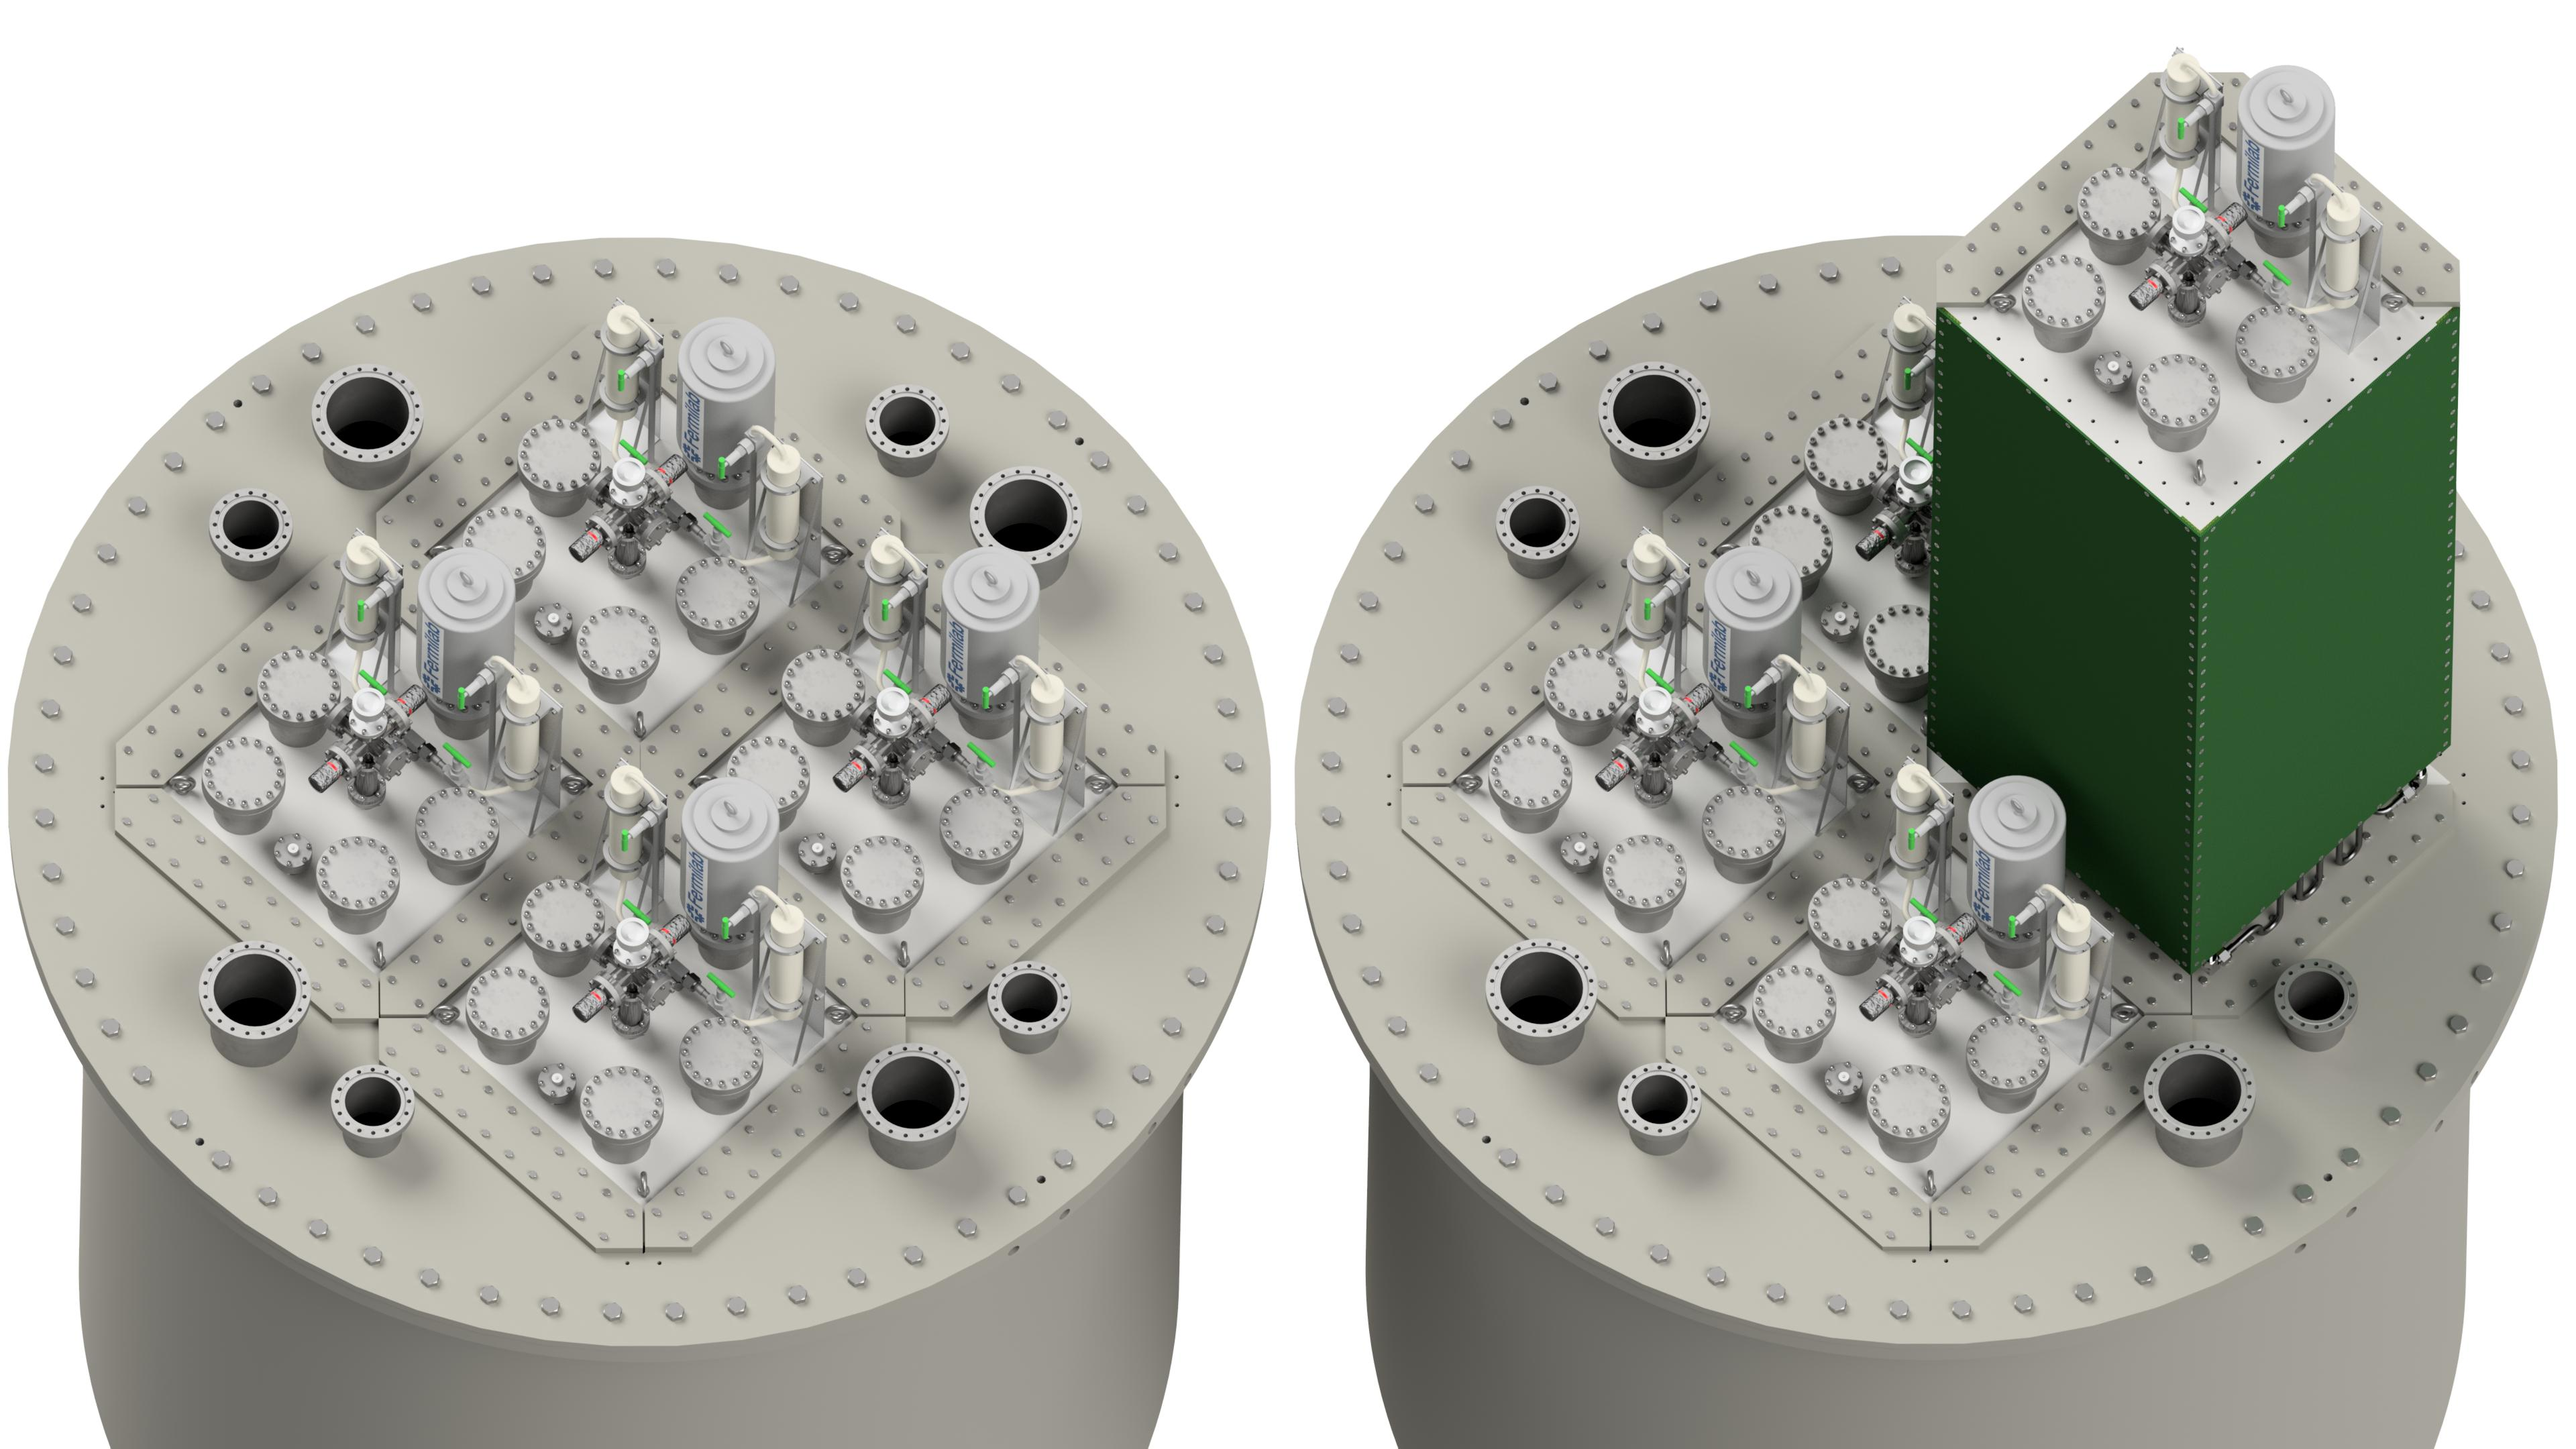
\includegraphics[width=\textwidth]{graphics/BathAndModule.jpeg}
	\caption{Illustration of the \dword{arcube} 2$\times$2 Demonstrator module. The four modules are visible, with one of them partly extracted, on the right. This figure has been reproduced from Ref.~\cite{argoncube_loi}.}
	\label{fig:2x2_extraction}
\end{figure}

Individual modules can be extracted or reinserted into a common \dword{lar} bath as needed, as is illustrated in Figure~\ref{fig:2x2_extraction}. This feature will be demonstrated during a commissioning run at the University of Bern, but is not intended to be part of the detector engineering studies in the \dword{minos}-\dword{nd} hall. The pressure inside the modules is kept close to the bath pressure, putting almost no hydrostatic force on the module walls.  This allows the walls to be thin, minimizing the quantity of inactive material in the walls. The purity of the \dword{lar} is maintained within the modules, independent of the bath, as will be described below. The argon surrounding the modules need not meet as stringent purity requirements as the argon inside. Under normal operating conditions, all modules are inserted with  clearance distances of only \SI{1.5}{\milli\metre} between modules. Cooling power to the bath is supplied by liquid nitrogen circulated through lines on the outer surface of the inner cryostat vessel.

\begin{figure}[tbp]
	\centering
	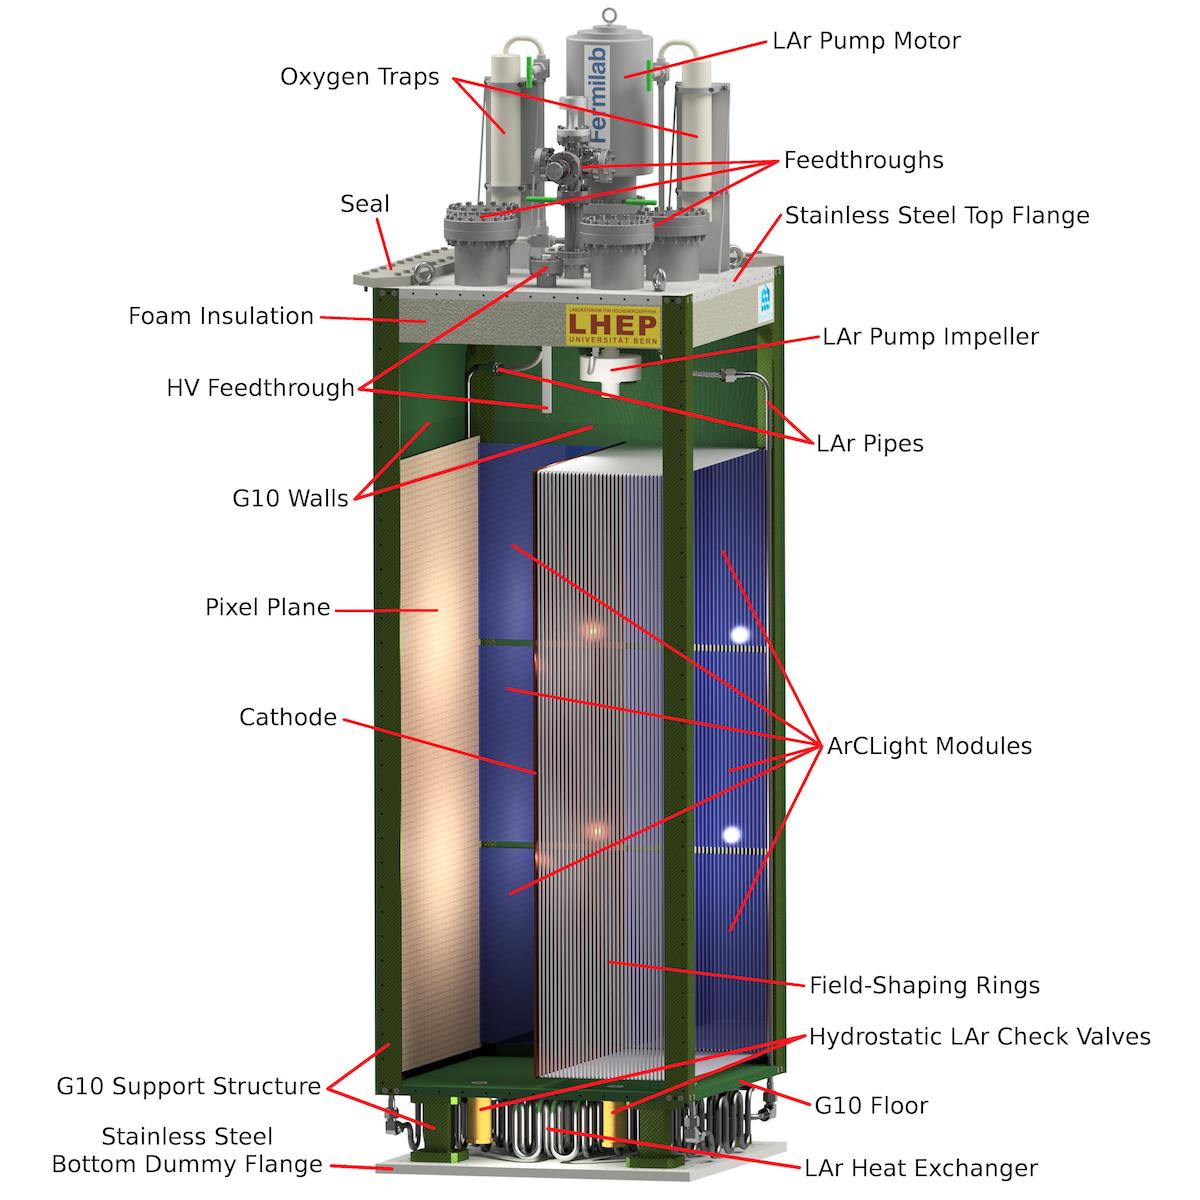
\includegraphics[width=0.8\textwidth]{graphics/Normal-Module-4K_labelled.jpeg}
	\caption[ArgonCube module engineering drawing]{Cutaway drawing of a \SI{0.67 x 0.67 x 1.81}{\metre} \dword{arcube} module for the 2$\times$2 Demonstrator module. For illustrative purposes the drawing shows traditional field shaping rings instead of a resistive field shell. Note, G10 walls will completely seal the module, isolating it from the neighbouring modules and the outer \dword{lar} bath.It is also worth noting that the 2$\times$2 modules will not have individual pumps and filters.}
	\label{fig:ac_module}
\end{figure}

A cutaway drawing of an individual 2$\times$2 module is shown in Figure~\ref{fig:ac_module}. The side walls of each module are made from \SI{1}{\centi\metre} G10 sheets, to which the resistive field shell is laminated. G10's electromagnetic radiation length ($X_{\mathrm{0}} = \SI{19.4}{\centi\metre}$) and hadronic interaction length ($\lambda_{\mathrm{int}} = \SI{53.1}{\centi\metre}$)~\cite{Tanabashi:2018oca} %Yao:2006px} 
are both comparable to \dword{lar} (14.0~cm and 83.7~cm respectively), making the G10 structures in the \dword{lar} almost transparent for passing particles. This results in a performance comparable to a monolithic detector. G10 provides a strong dielectric, capable of \SI{200}{\kilo\volt\per\centi\metre} when \SI{1}{\centi\metre} thick~\cite{G10Breakdown}. This dielectric shielding eliminates the need for a clearance volume between the \dwords{tpc} and the cryostat, while also shielding the \dword{tpc} from field breakdowns in a neighboring module. 

Each module is split into two \dwords{tpc} by a central cathode made of an additional resistive layer on a G10 substrate. The segmented drift length does not require a high cathode voltage, and minimizes stored energy. For the 2$\times$2 module footprint of \SI{0.67 x 0.67}{\metre}, and an \efield of \SI{1}{\kilo\volt\per\centi\metre}, a cathode potential of only \SI{33}{\kilo\volt} is required. Operating a \dword{lartpc} at this voltage is feasible without a prohibitive loss of active volume~\cite{Zeller:2013sva}.

The detector is oriented such that the cathodes are parallel to the beam. This minimizes the load on the readout electronics by spreading the event over more channels and reducing the required digitization rate for hit channels. In turn, this reduces the heat load generated at the charge readout and prevents localized boiling.

During filling and emptying of the cryostat, the argon flow is controlled by hydrostatic check valves located at the lower flange of the module, which require a minimal differential pressure of \SI{15}{\milli\bar} to open. The purity inside each module is maintained by means of continuous \dword{lar} recirculation through oxygen traps. Dirty argon is extracted from the base of the module, and is then pushed through oxygen traps outside the cryostat, clean argon then re-enters the module above the active volume. For optimal heat transport, the argon flow is directed along the cold electronics. To prevent dirty argon from the bath entering the modules, their interior is held at a slight overpressure. For the 2$\times$2, the dirty argon from all four modules is extracted by a single pump at the base of the cryostat with a four-to-one line, and after being filtered and cooled, the clean argon is pumped back in the module via a one-to-four line.
A more extensive version of the same scheme is envisaged for the \dword{dune} \dword{nd}.  


\dword{arcube} offers true \threed tracking information using the \dword{larpix} cryogenic \dword{asic}~\cite{larpix} pixelated charge readout. \dword{larpix} \dwords{asic} amplify and digitize the charge collected at single-pixel in the cold to mitigate the need for analogue signal multiplexing, thus produce unambiguous 3D information. Sixty-four pixels can be connected to a single \dword{larpix} \dword{asic}. The baseline design is for the 2$\times$2 is a \SI{4}{\milli\metre} pixel pitch, corresponding to 62.5k pixels m$^{-2}$. Pixelated anode planes are located on the two module walls parallel to the cathode; each plane is \SI[product-units=repeat]{1.28x0.64}{\metre\squared}. The total area across all four modules is \SI{6.6}{\metre\squared}, which corresponds to 410k pixels. The readout electronics utilize two FPGA boards per module, connected to a single Ethernet switch. It should be noted that the pixel pitch may be reduced as prototypes develop, but this can be accommodated in the readout design. 

\begin{figure}[!ht]
	\centering
	\subfloat[\dword{arclt} paddle] {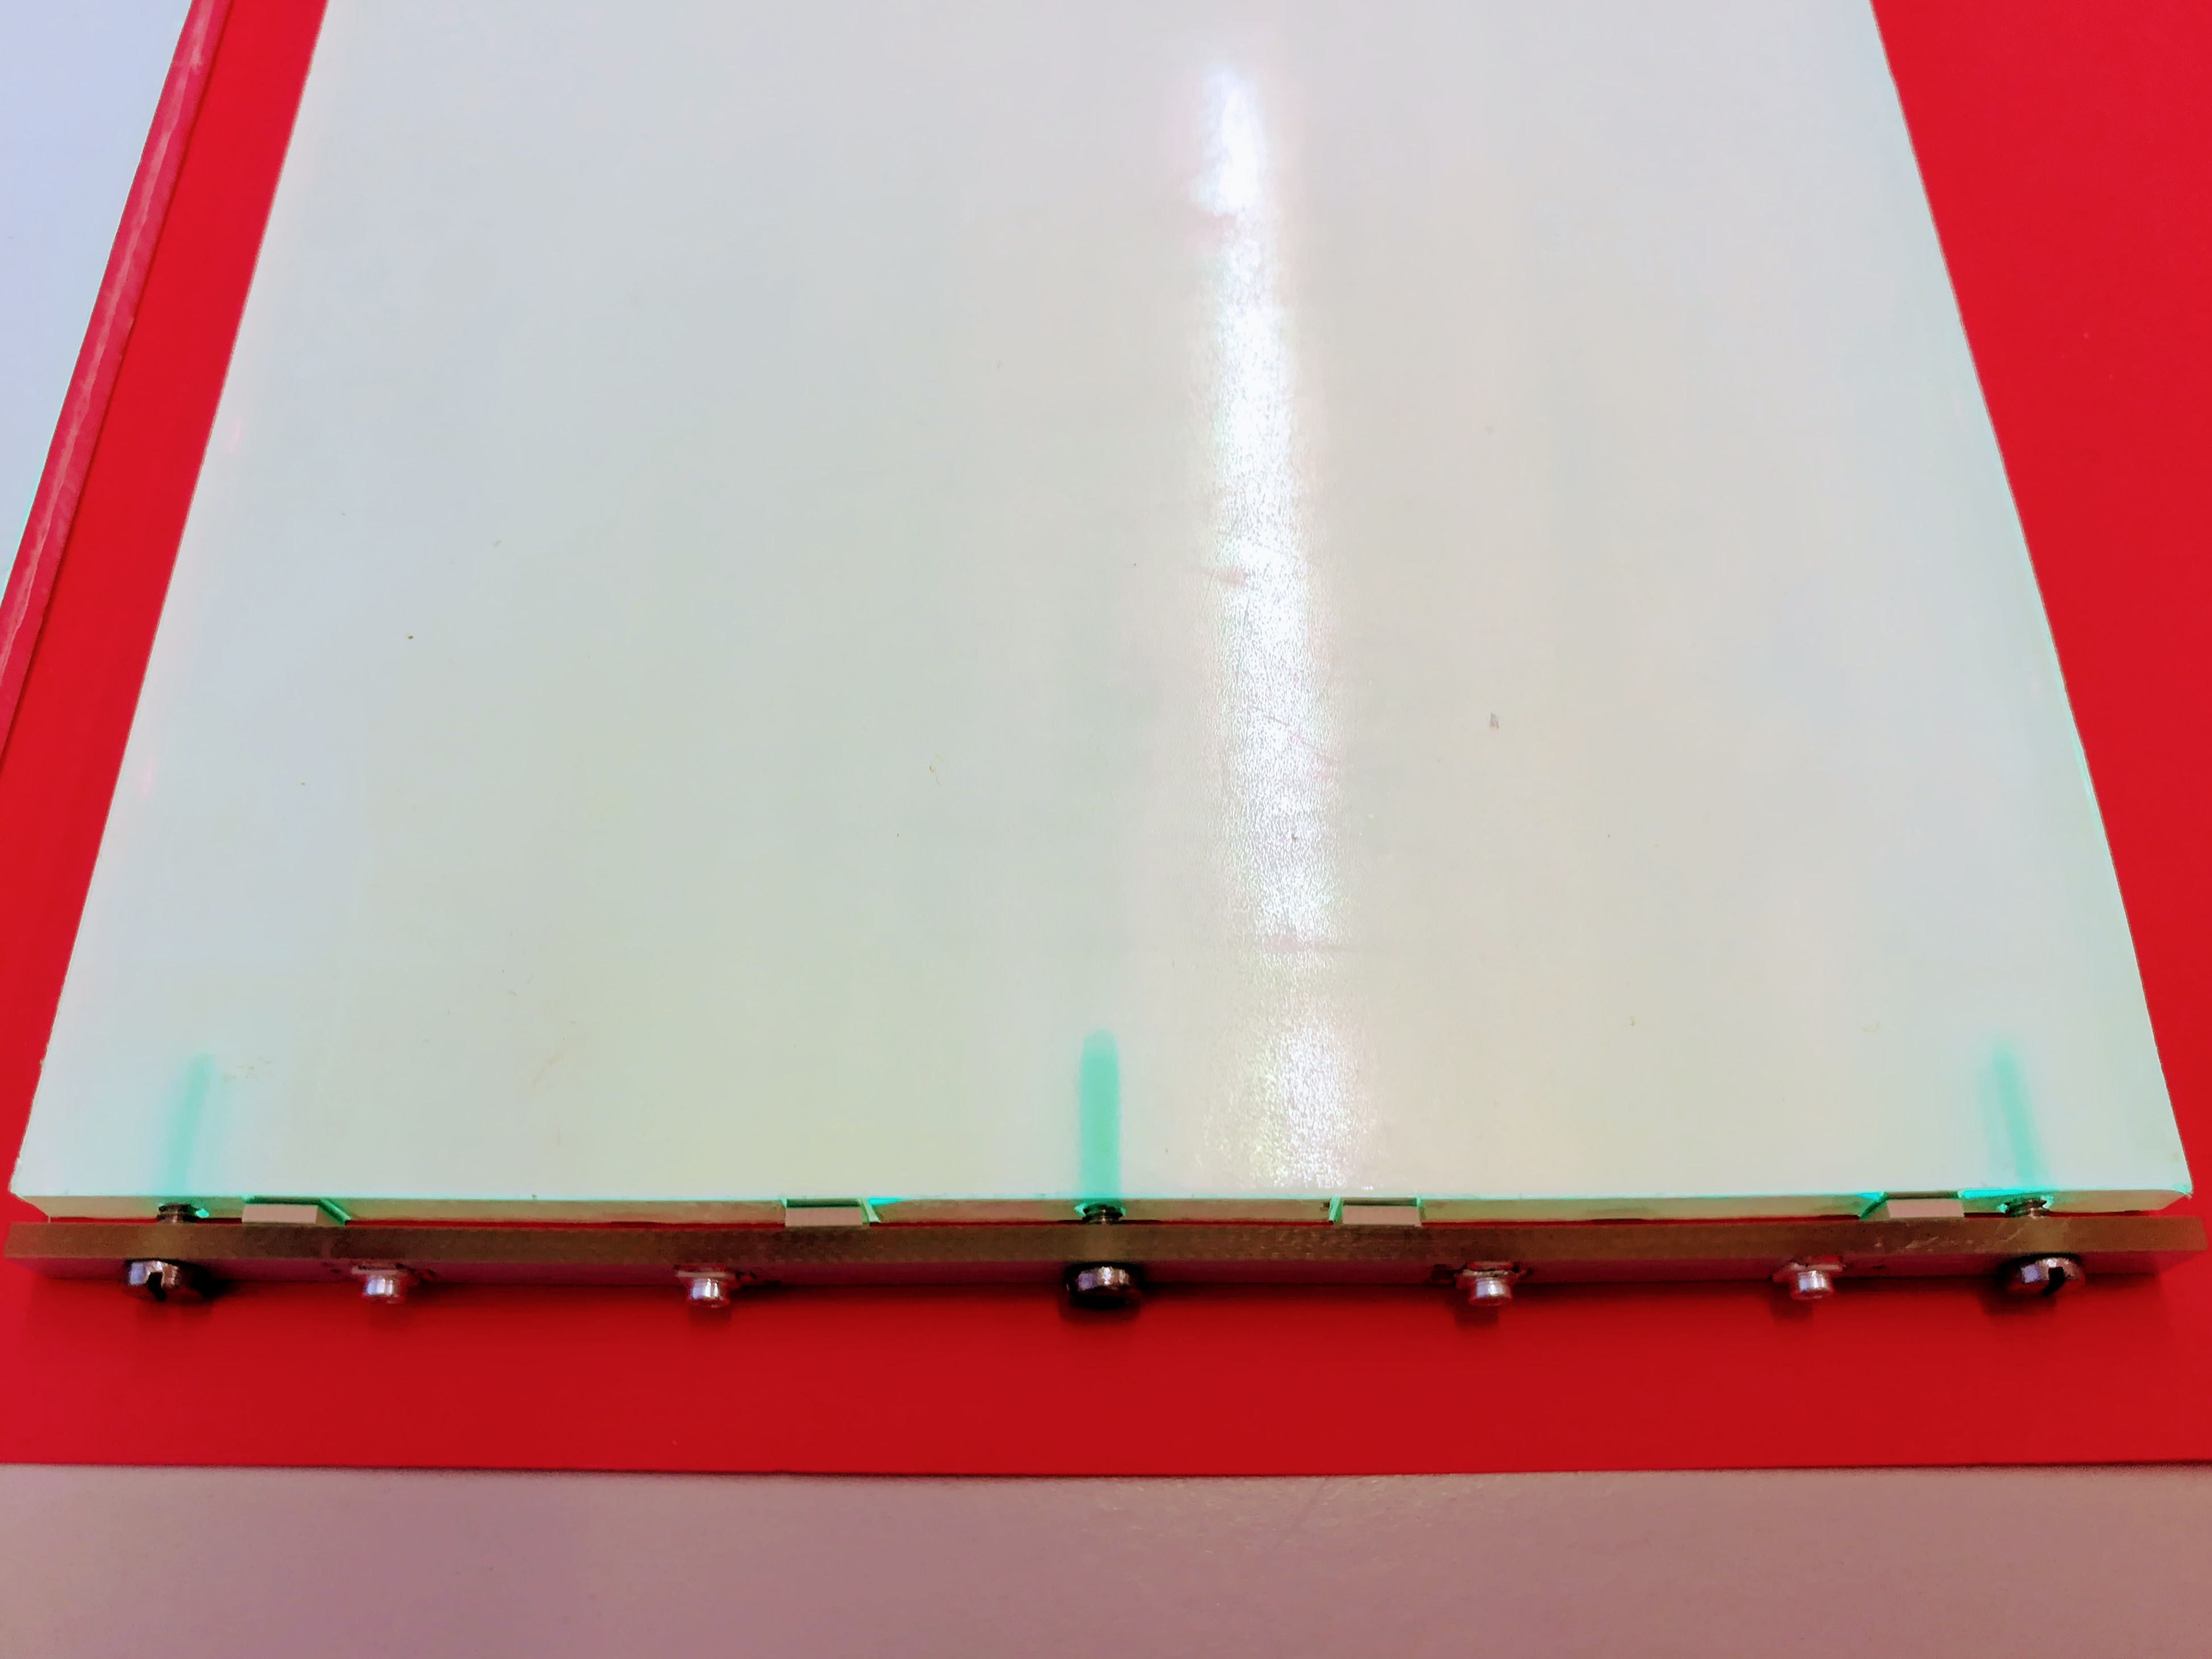
\includegraphics[width=0.454\textwidth]{graphics/arclight.jpg}}
	\subfloat[\dword{arclt} mounted on a pixel readout PCB]  {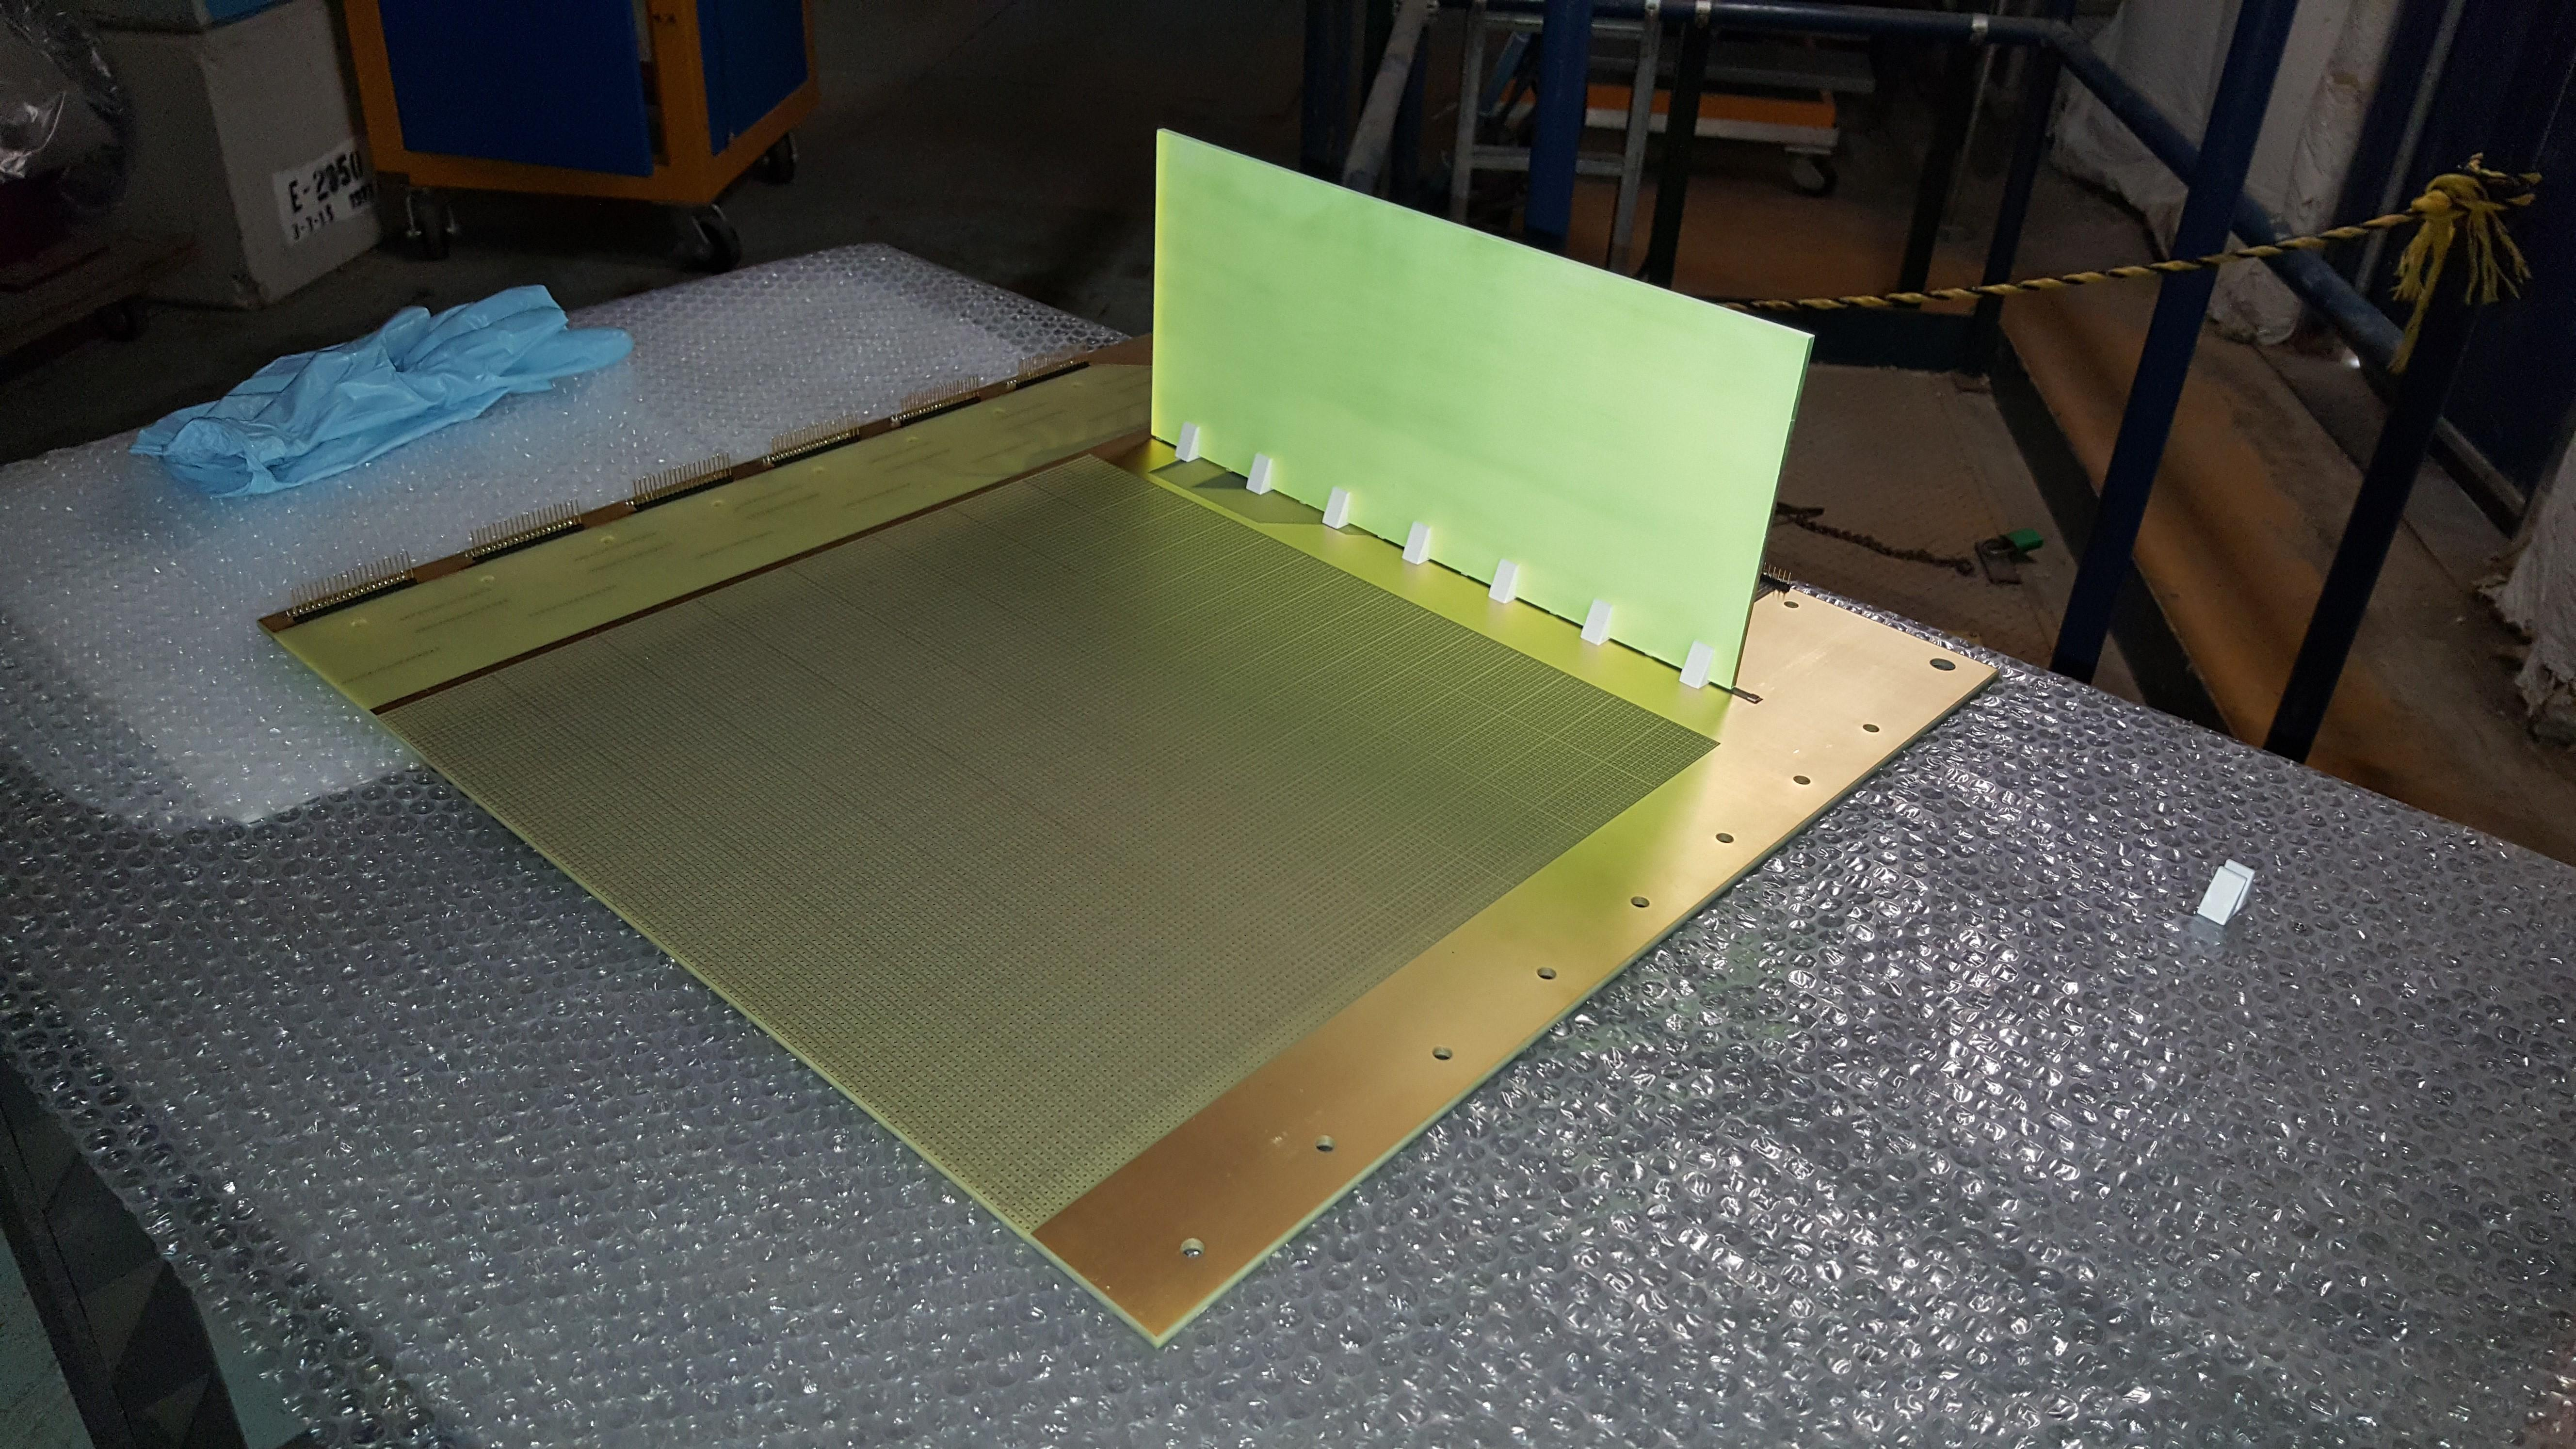
\includegraphics[width=0.51\textwidth]{graphics/Pixlar.jpeg}}
	\caption{(a) A prototype ArgonCube light readout paddle built at the University of Bern. The paddle is 50~cm long and 10~cm wide, with four SiPMs coupled to one end. Reproduced from Ref.~\cite{argoncube_loi}. (b) ArClight paddle mounted on the PixLAr pixelated charge readout plane, as used in test beam studies at Fermilab.}
	\label{fig:arclight}
\end{figure}

The charge readout window (drift time) of \SI{137}{\micro\second} is long compared to the \SI{10}{\micro\second}~\cite{Adamson:2015dkw} beam spill length in the \dword{numi} and \dword{lbnf} beams.
For a \SI{1}{MW} beam intensity, the expected rate of neutrino interactions at the \dword{dune} \dword{nd} is roughly 0.5 per spill per \dword{arcube} module.  
With \dword{larpix}, reconstruction issues are greatly simplified compared to a projective readout \dword{tpc}.
Tracks and connected energy deposits will frequently overlap in any 2D projection, but can be easily resolved with the full \threed readout.
However, disconnected energy deposits, such as those from photon conversions or neutron interactions in the detector, cannot be easily associated to a specific neutrino interaction.
This problem can be solved by incorporating fast timing information from the prompt scintillation light emitted in \dword{lar}.
The module's opaque cathode and walls contain scintillation light within each \dword{tpc} (half module), improving the detection efficiency of the prompt component of the scintillation light. 
Furthermore, attenuation due to Rayleigh scattering, characterized by an attenuation length of \SI{0.66}{\metre} in \dword{lar}~\cite{Grace:2015yta}, is mitigated by the maximum photon propagation length of \SI{0.3}{\metre}. 
It is desirable to have a large area photon detection system to maximize the utility of scintillation light signals in the detector. 
To minimize any dead material within the active volume, it is also desirable that the light detection be as compact as possible. 
The solution pursued for the \dword{arcube} effort is \dword{arclt}~\cite{Auger:2017flc}, which is a very compact dielectric light trap that allows for light collection from a large area, inside high electric fields. 
An example \dword{arclt} sheet is shown in Figure~\ref{fig:arclight}. These sheets are mounted on the walls of the module, inside the field shell, aligned with the drift direction, between the anode and the cathode. 
The additional \SI{5}{\milli\metre} deep dead volume is similar to the one caused by the charge readout in the perpendicular direction.

\subsection{Dimensions of the ArgonCube Component of the DUNE  ND}\label{sec:had_containment}

Since it is unrealistic to build a \SI{25}{\metre} long \dword{lartpc} in order to contain a \SI{5}{\giga\electronvolt} muon, the \dword{lartpc} dimensions have instead been optimized for hadronic shower containment~\cite{lartpcSizeChris}, relying on a downstream spectrometer to analyze crossing muons.
Hadronic showers are defined as contained if a reasonable efficiency across a wide range of kinematics is maintained, and there is no phase space with zero acceptance. 
The specific metric used is that \textgreater95\% of hadronic energy has to be contained, excluding neutrons and their descendants.

To assess the efficiency, detector volumes of varying sizes were simulated in a neutrino beam.
This provides a good measure of the efficiency of a given volume to contain different events, but it is not necessarily a good quantity to assess the required detector size.
Many events are not contained because of their specific location and/or orientation.
Cross section coverage remedies this deficiency by looking at the actual extent of the event, instead of its containment, at a random position inside a realistic detector volume.
However, events extending through the full detector will very likely never be contained in a real detector due to the low probability of it happening in exactly the right location (e.g., at the upstream edge of the detector).
Therefore, the maximum event size needs to be smaller than the full detector size.
For the \dword{nd} simulation this buffer was chosen to be \SI{0.5}{\metre} in all directions.
In this way, this measure of cross section coverage allows us to look for phase-space regions which are inaccessible to particular detector volume configurations.

To find the optimal detector size in each dimension, two are held constant at their nominal values, while the third dimension is varied and the cross section coverage is plotted as a function of neutrino energy. 
This is shown for the dimension along the beam direction in Figure~\ref{fig:dune-nd_lartpc-size}. In this case, Figure~\ref{fig:dune-nd_lartpc-size} shows us that
\SI{4.5}{\metre} would be sufficient, but to avoid model dependencies, \SI{5}{\metre} has been selected.
Increasing the length beyond \SI{5}{\metre} does little to improve cross section coverage, but reducing to \SI{4}{\metre} begins to limit coverage at higher energies.
Note that 1 minus the cross section coverage gives the fraction of events that cannot be well reconstructed no matter where their vertex is, or how they are rotated within the fiducial volume. The optimized dimensions found using this technique were \SI{3}{\metre} tall, \SI{4}{\metre} wide, and \SI{5}{\metre} along the beam direction.

\begin{figure}[tbp]
	\centering
	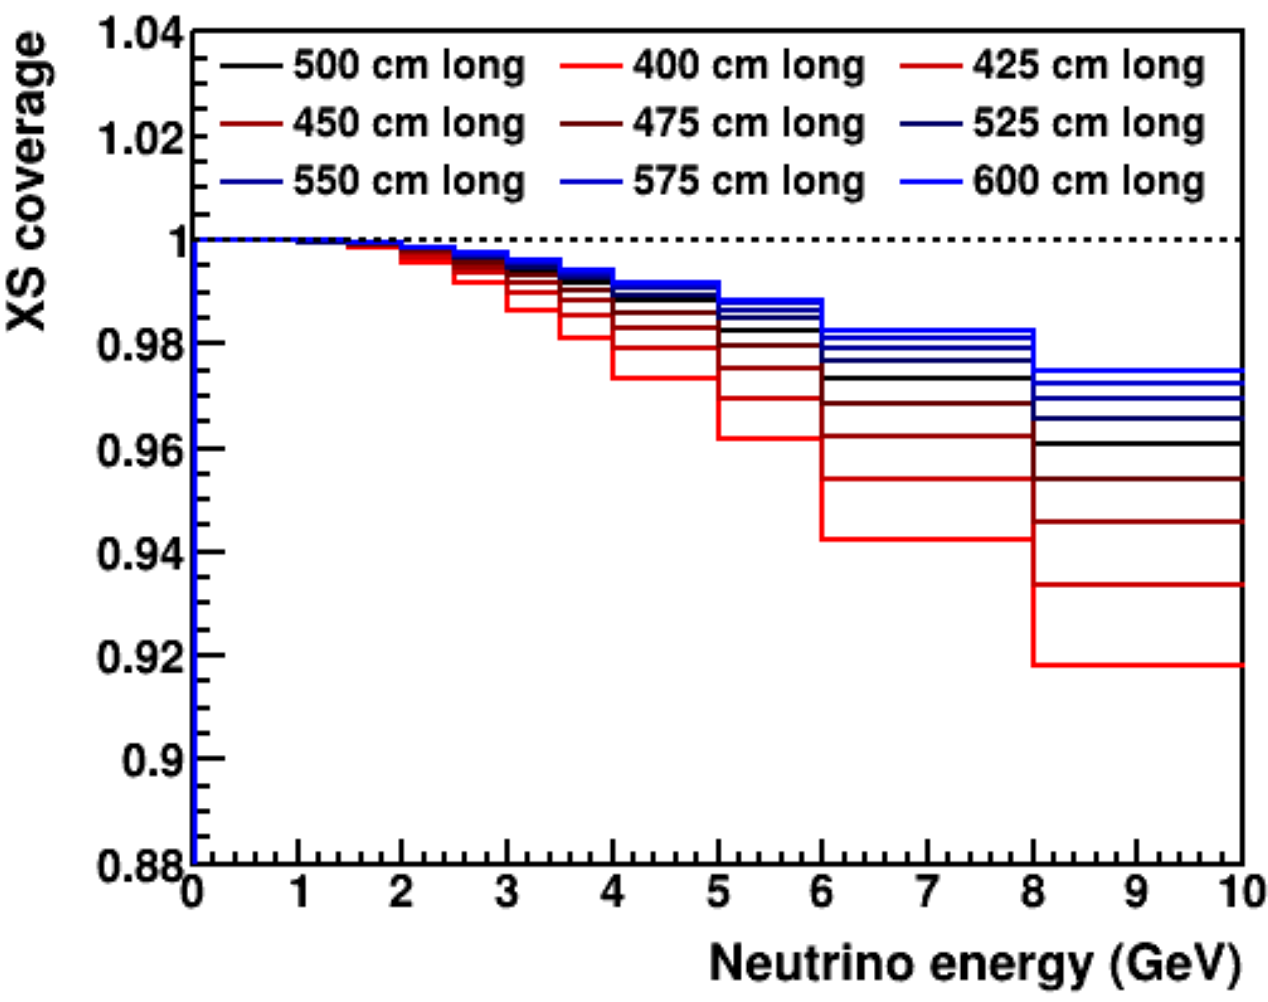
\includegraphics[width=0.5\textwidth]{graphics/length.png}
	\caption{Influence of the \dword{lartpc} size on hadron containment, expressed in terms of cross section coverage as a function of neutrino energy.
		Two dimensions are held constant at their nominal values, while the third is varied, in this case the height is held at \SI{2.5}{\metre} and the width at \SI{4}{\metre}.
		The optimal length is found to be \SI{5}{\metre}.
		See text for explanation of cross section coverage~\cite{lartpcSizeChris}.}
	\label{fig:dune-nd_lartpc-size}
\end{figure}


%\subsection{Module Dimensions}
\subsection{ArgonCube Module Dimensions}

The \dword{dune}  \dword{nd} \dword{arcube} module dimensions are set to maintain a high drift field, \SI{1}{\kilo\volt\per\centi\metre}, with minimal bias voltage, and to allow for the detection of prompt scintillation light while mitigating the effects of diffusion on drifting electrons.
The prompt scintillation light, $\tau<$\SI{6.2}{\nano\second}~\cite{Heindl:2015yaa}, can be efficiently measured with a dielectric light readout with $\mathcal{O}\left(1\right)\,\mathrm{ns}$ timing resolution, such as \dword{arclt}~\cite{Auger:2017flc}.
To reduce attenuation and smearing due to Rayleigh scattering, the optical path must be kept below the \SI{0.66}{\metre}~\cite{Grace:2015yta} scattering length.   Additionally, the slow scintillation component can be further suppressed by operating at higher \efield{}s~\cite{PhysRevB.20.3486}, effectively reducing the ionization density~\cite{PhysRevB.27.5279} required to produce excited states. 

A module with a \SI{1x1}{\metre} footprint split into two \dwords{tpc} with drift lengths of \SI{50}{\centi\metre} requires only a \SI{50}{\kilo\volt} bias.
With \dword{arclt} mounted either side of the \SI{1}{\metre} wide \dword{tpc}, the maximal optical path is only \SI{50}{\centi\metre}.
For a non-zero drift field, diffusion needs to be split into longitudinal and transverse components. Gushchin~\cite{gushchin} report a transverse diffusion of \SI{13}{\centi\metre\squared\per\second} at \SI{1}{\kilo\volt\per\centi\metre}.
This results~\cite{lngDet} in a transverse spread of \SI{0.8}{\milli\metre} for the drift time of \SI{250}{\micro\second}, well below the the proposed pixel pitch of \SI{3}{\milli\metre}.
The longitudinal component is smaller than the transverse ~\cite{lngDet},  and is therefore negligible.

%\subsection{Detector Dimensions}
\subsection{ND Dimensions}
\label{sec:det_dimensions}

%Given that the space transverse to the beam is not a constrained commodity in the \dword{nd} hall, 
Though the acceptance study discussed in Section~\ref{sec:had_containment} indicated a width of \SI{4}{\metre} is sufficient to contain the hadronic component of most events of interest, the width has been increased to 
\SI{7}{\metre} in order to mitigate the need for a side-going muon spectrometer.
Figure~\ref{fig:actual-size} shows the overall dimensions of the planned \dword{arcube} deployment in the \dword{dune}  \dword{nd}. 
With an active volume of \SI{1x1x3}{\metre} per module, the full \dword{arcube} detector corresponds to seven modules transverse to the beam direction, and five modules along it. 
It should be noted that the cryostat design is currently based on \dword{protodune}~\cite{Abi:2017aow}, and will be optimized for the  \dword{nd} pending a full engineering study.  

\begin{figure}[tbp]
	\centering
	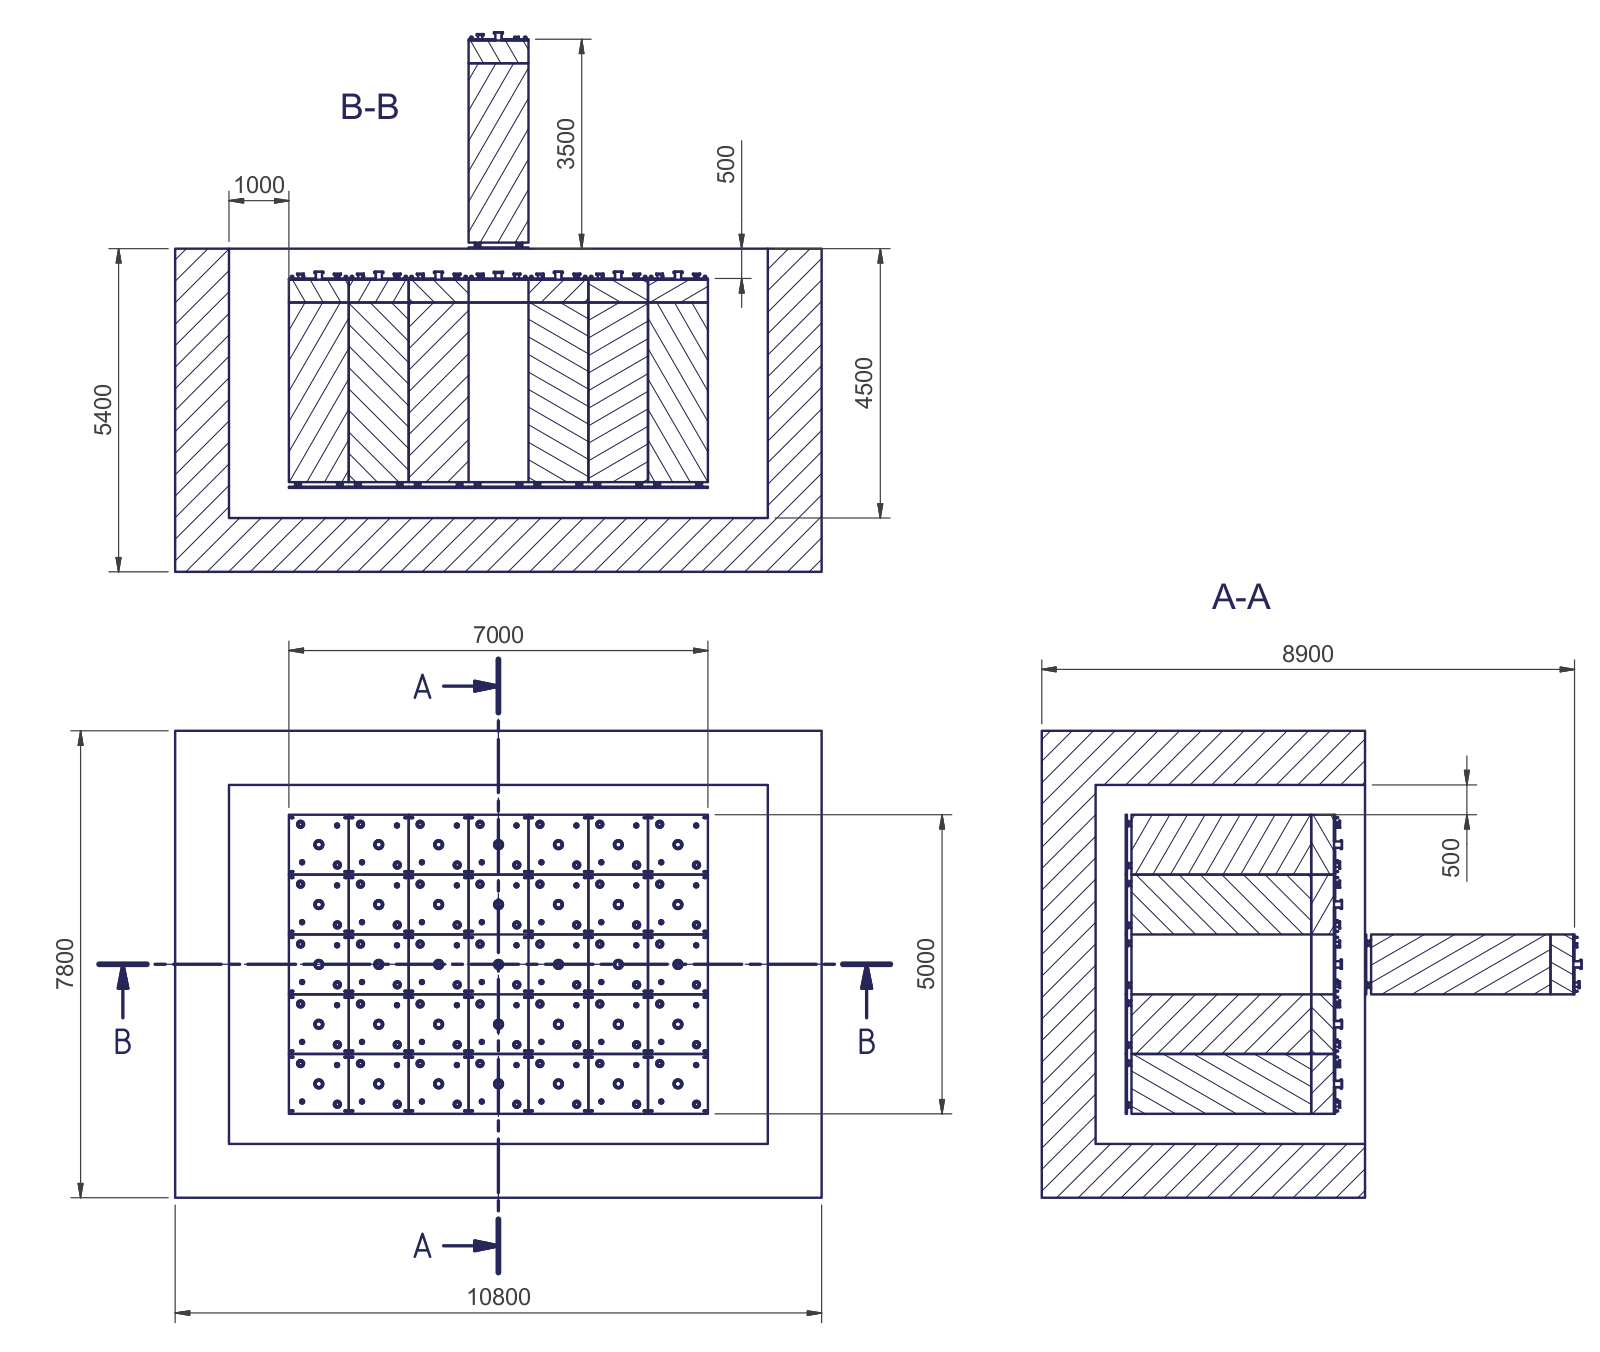
\includegraphics[width=0.7\textwidth]{graphics/actual-size.png}
	\caption{The current \dword{arcube} Dimensions for the \dword{dune}  \dword{nd}. The cryostat is based on \dword{protodune}~\cite{Abi:2017aow}, and yet to be optimized for the \dword{dune}  \dword{nd}.}
	\label{fig:actual-size}
\end{figure}


\subsubsection{Statistics in Fiducial Volume}\label{sec:rates}

Figure~\ref{fig:all_ey} shows 37 million total \dword{cc} $\numu$ neutrino events per year within a \SI{25}{\tonne} fiducial volume in \dword{fhc} mode at \SI{1.07}{\mega\watt}. Figure~\ref{fig:hadContNorm_ey} shows only the event rate for events where the visible hadronic system is fully contained, for the same fiducial volume and beam configuration. Note that for the visible hadronic system to be contained, all energy not associated with the outgoing lepton, or outgoing neutrons, was required to be contained. 


For hadronic containment, there is a \SI{30}{\centi\metre} veto region upstream and on all sides of the active volume, and \SI{50}{\centi\metre} veto region downstream. The fiducial volume is then defined as \SI{50}{\centi\metre} from all edges, with \SI{150}{\centi\metre} downstream.  Within the \SI{25}{\tonne} fiducial volume in \dword{fhc} mode at \SI{1.07}{\mega\watt} the number of fully reconstructed (contained or matched muon, discussed below, plus contained hadrons) \dword{cc} $\numu$ events per year is 14 million.   

\begin{figure}[tbp]
	\centering
	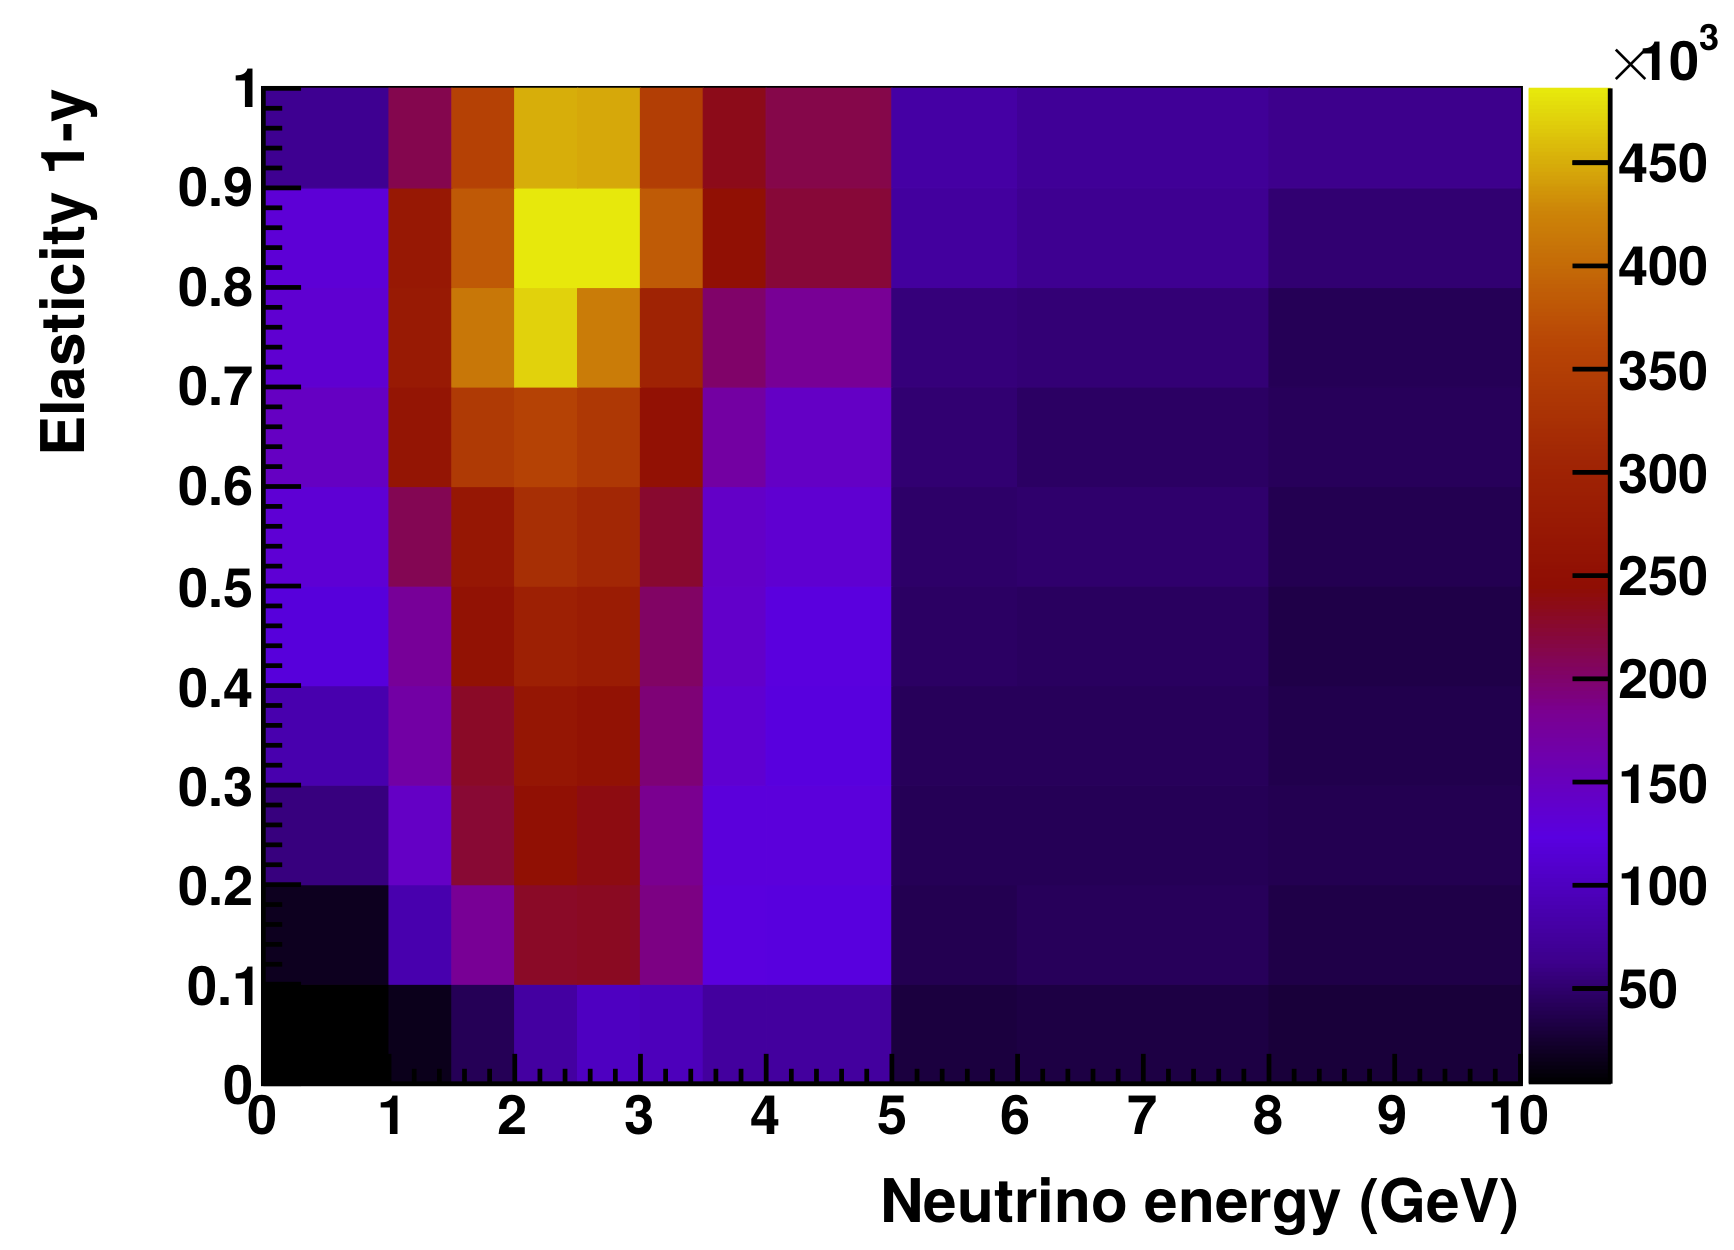
\includegraphics[width=0.6\textwidth]{graphics/all_ey.png}
	\caption{All neutrino events in the nominal \SI{25}{\tonne} fiducial volume, in \dword{fhc} at \SI{1.07}{\mega\watt}, per year, rates are per bin.}
	\label{fig:all_ey}
\end{figure}

\begin{figure}[tbp]
	\centering
	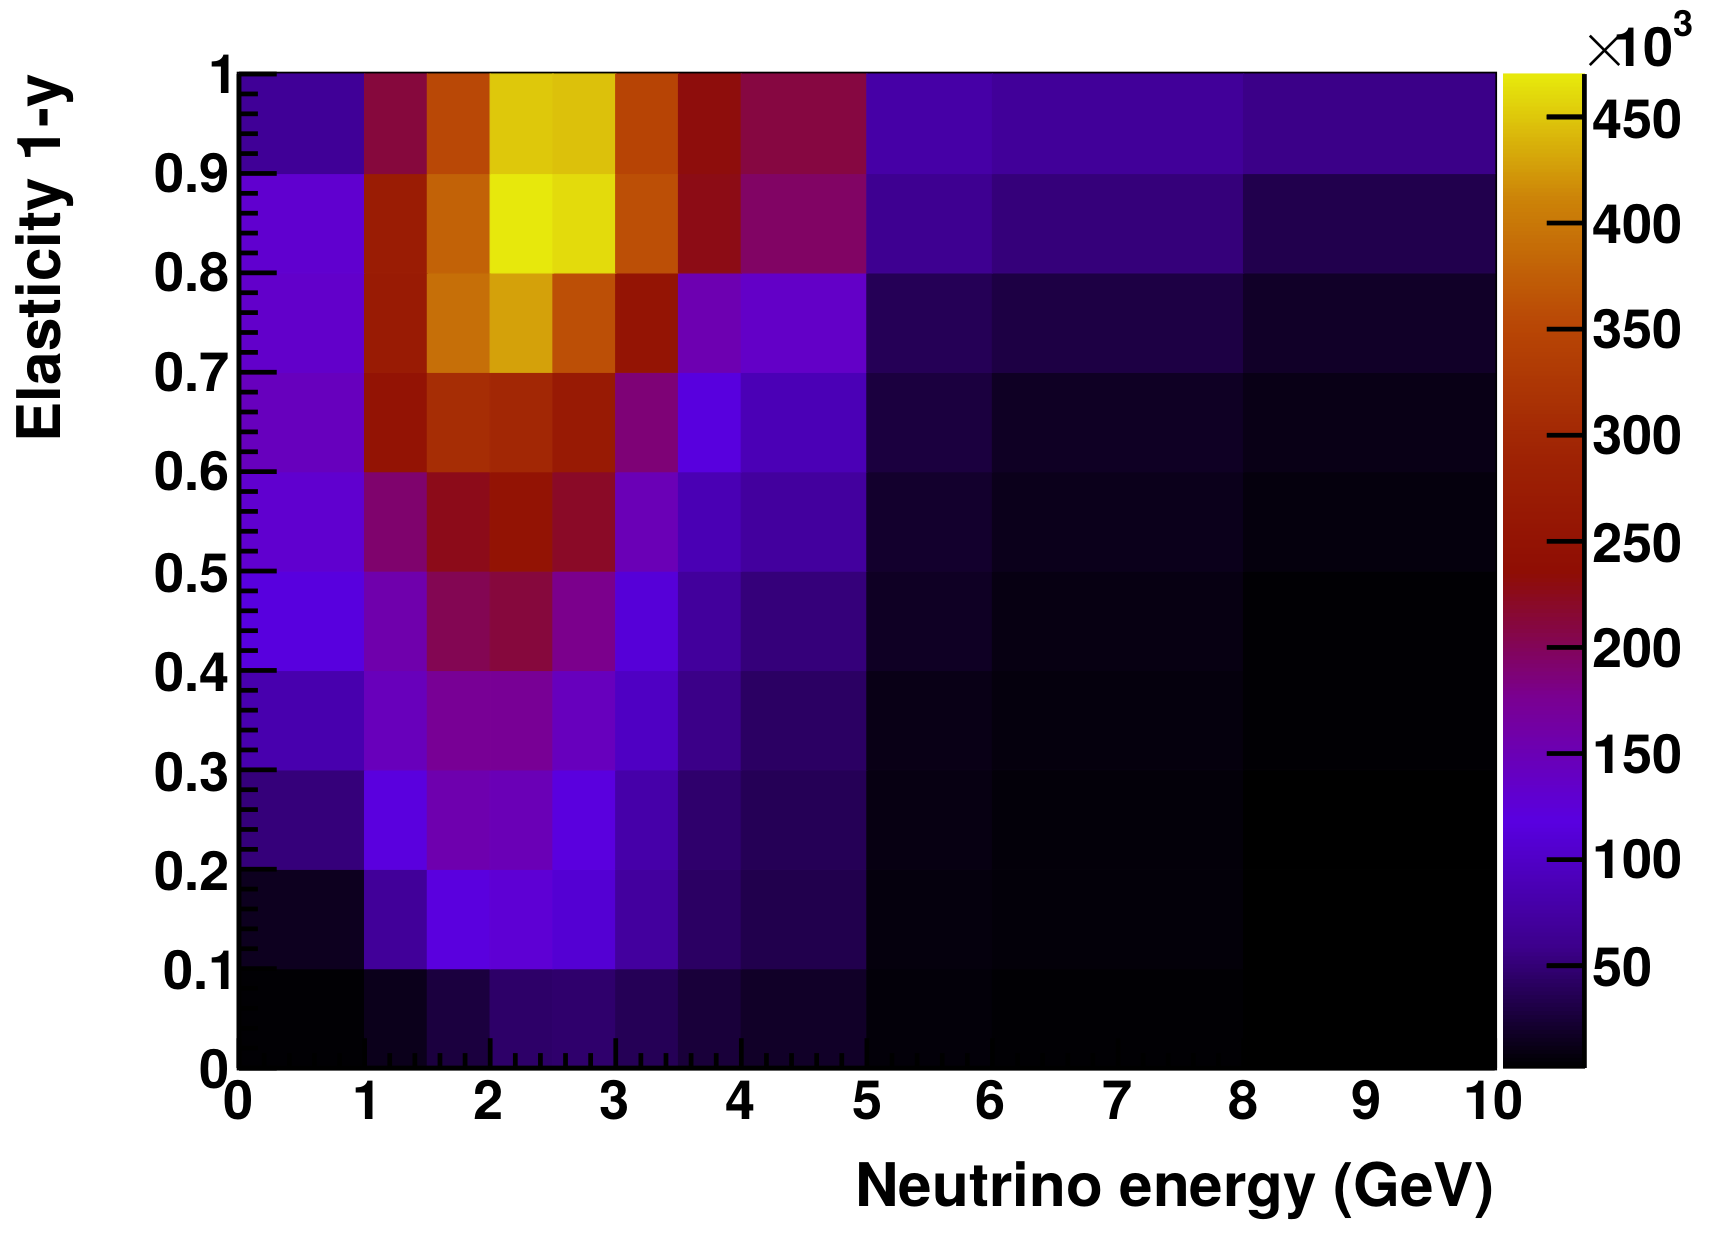
\includegraphics[width=0.6\textwidth]{graphics/hadContNorm_ey.png}
	\caption{Events where the visible hadronic system is contained within the nominal \SI{25}{\tonne} fiducial volume, in \dword{fhc} at \SI{1.07}{\mega\watt}, per year, rates are per bin.}
	\label{fig:hadContNorm_ey}
\end{figure}

\subsubsection{Muon Acceptance}\label{sec:muacc}

Muons are considered as useful for physics if they stop in the active region of \dword{arcube} or if they leave the \dword{lar} detector and are reconstructed in a magnetic spectrometer downstream.  Under the assumption that the downstream magnetic spectrometer is the multipurpose detector described in section~\ref{sec:exsum-nd-mpt}, Figure~\ref{fig:muonacc}  shows the muon acceptance as a function of true neutrino energy (on the left) and muon energy (on the right). The acceptance dip at \SI{1}{GeV} in muon energy is from muons that exit \dword{arcube} and are not reconstructed in the \dword{mpd} downstream.

\begin{figure}[h!]
   \begin{center}
      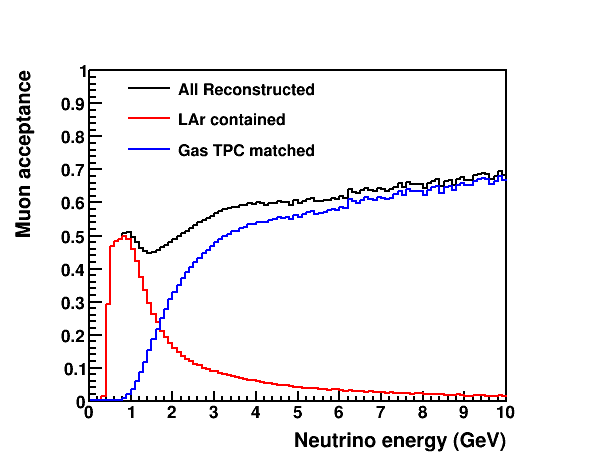
\includegraphics[width=0.45\textwidth]{muReco_Ev.png}
      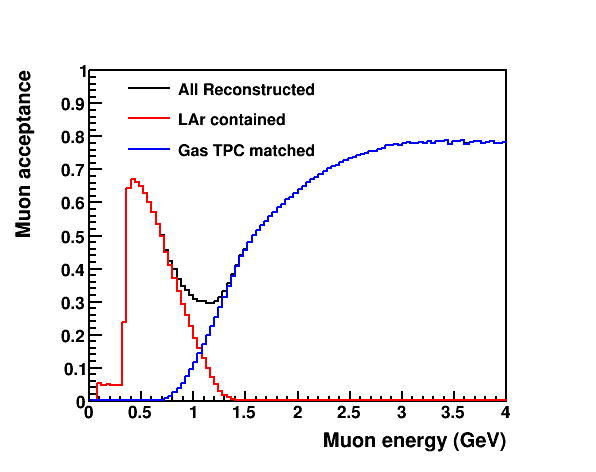
\includegraphics[width=0.45\textwidth]{muReco_Emu.png}
      \caption{Muon acceptance shown as a function of true neutrino energy (left) and true muon energy (right).  The acceptance for muons that stop in \dword{arcube} is shown in red and that for muons reconstructed in the downstream magnetic spectrometer is shown in blue.}
      \label{fig:muonacc}
   \end{center}
\end{figure}

\subsection{Muon and Electron Momentum Resolution and Scale Error}

%This has not yet been investigated fully 

For muons stopping in the \dword{lar} and for those with momentum measured in the downstream tracker (\dword{mpd}), the energy scale uncertainty from \dword{arcube} is driven by the material model of the \dword{lar} and passive materials.  This is expected to be known to \textless 1\%.
%It is hard to imagine getting the energy loss in LAr wrong in a systematic way. The uncertainty due to the passive materials is basically just how well the composition is known, which is probably \textless 1\%.

For electrons, the energy will be measured calorimetrically, rather than by range.  The \dword{mip} energy scale (Q/MeV) will be set by rock muons.  The scaling to more dense deposits from EM showers can give rise to uncertainties, i.e., recombination could be different.  Such uncertainties can be reduced by taking data with \dword{arcube} modules in a test beam.  Outside of this, a useful calibration sample
of electrons up to \SI{50}{MeV} comes from Michel electrons from stopping rock muons. The $\pi^0$ invariant mass peak is another good standard candle.



\subsection{Tagging Fast Neutrons}

Studies have shown that contained prompt scintillation light provides an important handle for neutron tagging, allowing for the association of detached energy deposits to the correct neutrino interaction using timing information. Such neutron tagging is important for minimizing the uncertainty on neutrino energy reconstruction, both for neutrons generated at a neutrino vertex and for hadronic showers that fluctuate to neutrons. 

Figure~\ref{fig:NDSpill} shows a simulated beam spill in the \SI[product-units=repeat]{5x4x3}{\metre} \dword{lar} component of the \dword{dune}  \dword{nd}\footnote{Note that this study was performed before the detector width was increased to \SI{7}{m}, as described in Section~\ref{sec:det_dimensions}.}. 
It highlights the problem of associating fast-neutron induced energy deposits to a neutrino vertex using only collected charge.  

\begin{figure}[htb]
	\centering{
		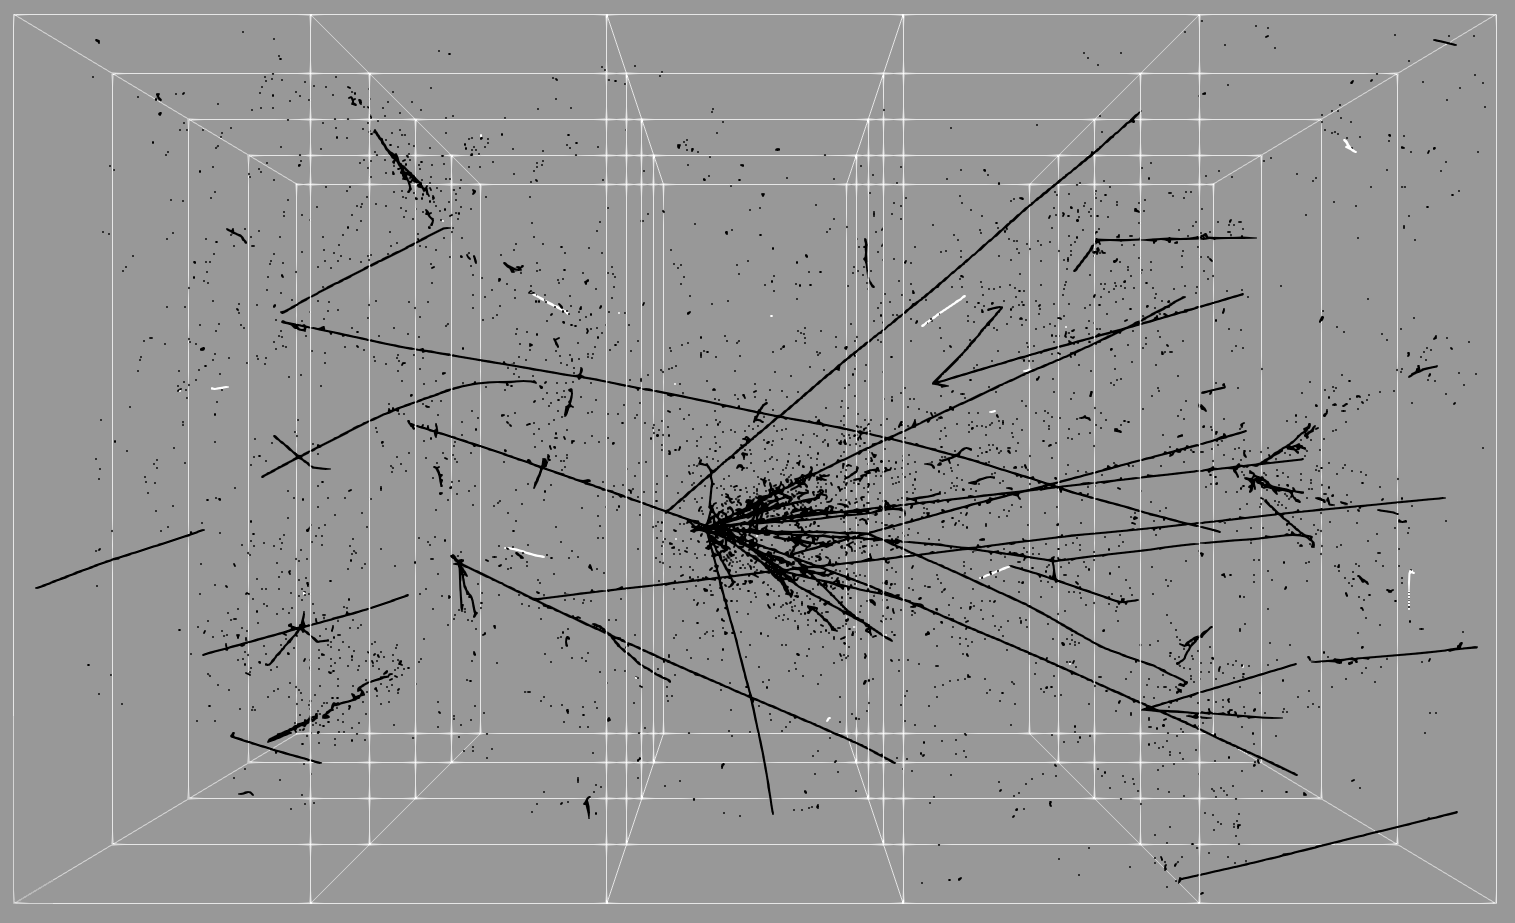
\includegraphics[width=.7\textwidth]{graphics/NeutronNDSpill.png}
	}
	\caption{A beam spill in the \dword{lar} component of the \dword{dune} ND. 
		The detector volume is \SI[product-units=repeat]{5x4x3}{\metre}.
		Fast-neutron induced recoiling proton tracks, with an energy threshold greater than $\sim\,$\SI{10}{\mega\electronvolt}, are shown in white.
		The black tracks are all other energy deposits sufficient to cause charge collected at the pixel planes.}
	\label{fig:NDSpill}
\end{figure}

By containing scintillation light, prompt light signals can be used to associate fast-neutron induced deposits back to a neutrino vertex anywhere within the detector.
Figure~\ref{fig:Timing} shows the temporal distribution of neutrino vertices within a beam spill.
The mean separation of neutrino vertices is \SI{279}{\nano\second}, with all fast-neutron induced energy deposits occurring $<$\SI{10}{\nano\second} after each neutrino interaction.      

\begin{figure}[htb]
	\centering{
		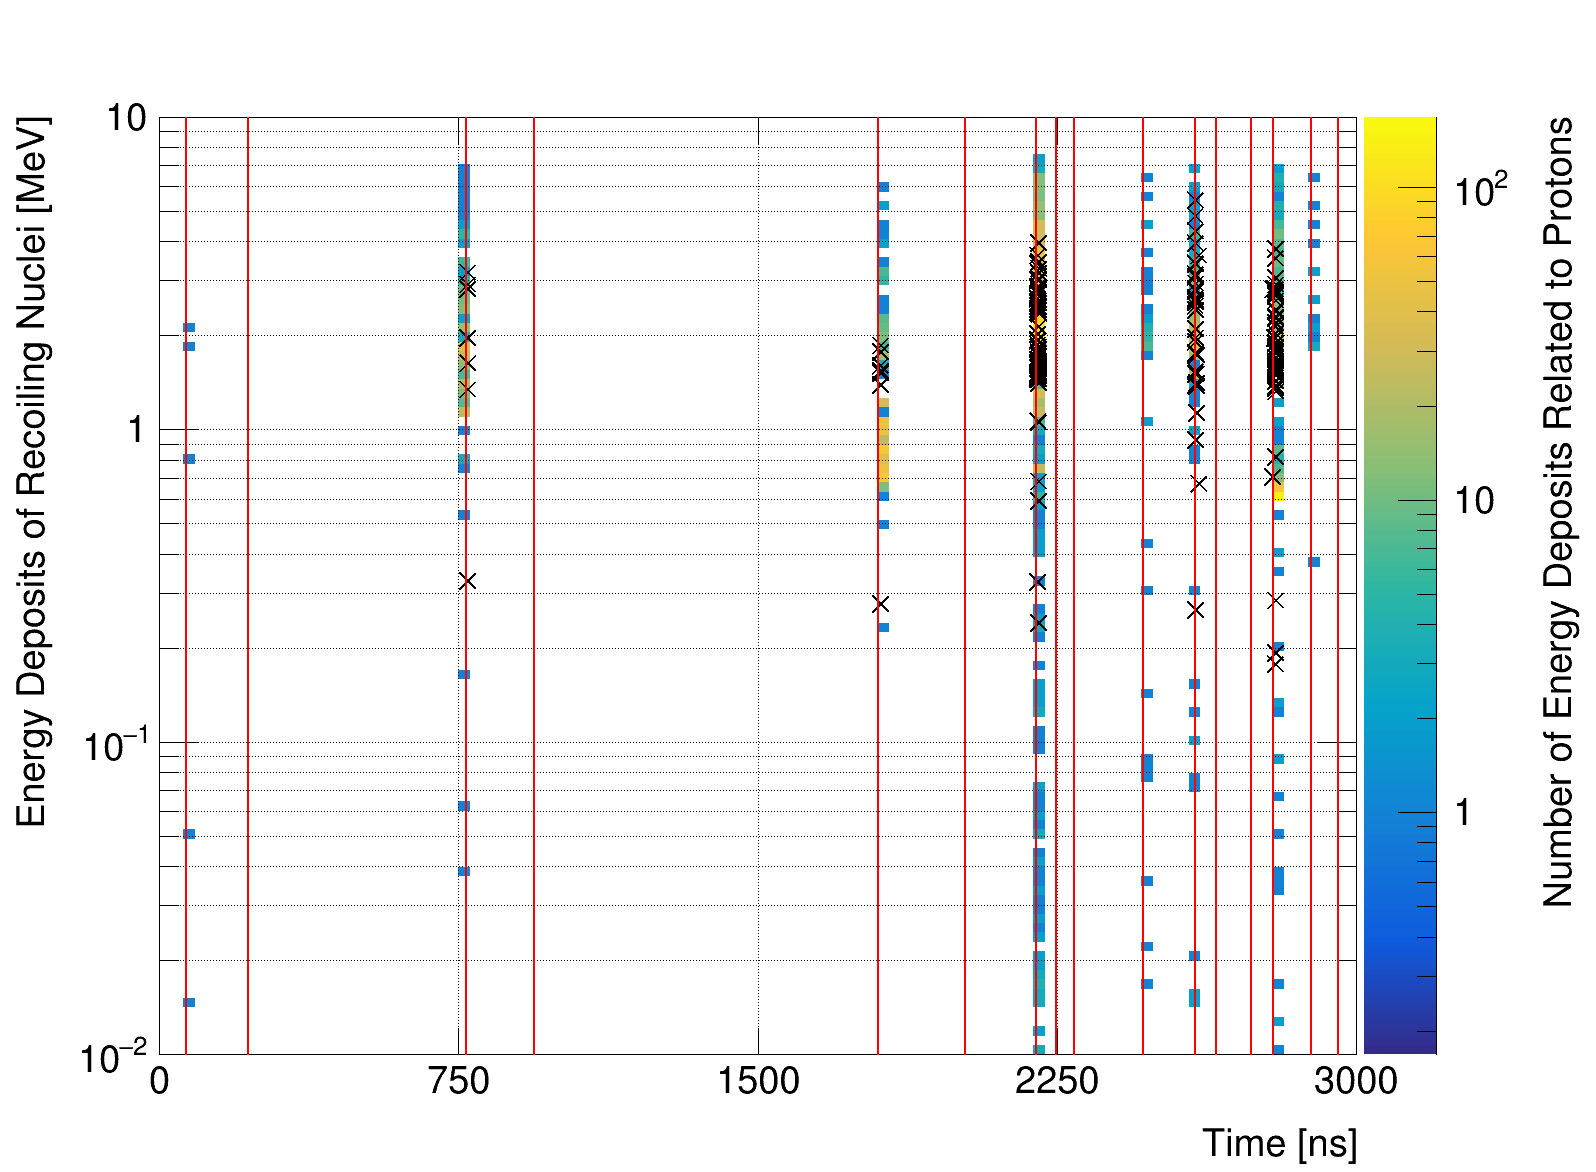
\includegraphics[width=0.7\textwidth]{graphics/recoil_proton_edep_vs_vtx_time_a.png}
	}
	\caption{The temporal distribution of neutrino vertices (red lines) within a beam spill in the \dword{lar} component of \dword{dune} ND.
		The mean separation of neutrino vertices is \SI{279}{\nano\second}. The filled bins show the number of hits due to recoiling protons, crosses indicate a hit due to a recoiling $^{2}$H, $^3$H, $^2$He or $^3$He nucleus.
		All fast-neutron induced energy deposits occur $<$\SI{10}{\nano\second} after each neutrino interaction.}
	\label{fig:Timing}
\end{figure}

	
\subsection{Neutrino-Electron Elastic Scattering}
\label{ssec:lartpc-nu-electron-scatt}

Neutrino scattering on atomic shell electrons, $\nu_{l}(\overline{\nu}_{l}) + e^{-} \rightarrow \nu_{l}(\overline{\nu}_{l}) + e^{-}$,
is a purely electroweak process with a known cross section as function of neutrino energy, $E_{\nu}$, in which all (anti)neutrino flavors participate, albeit with different cross sections. This process is independent of the nucleus interactions and has a clean signal of a single very forward-going electron. \dword{minerva}~\cite{Park:2015eqa} has used this technique to characterize the \dword{numi} beam flux normalization (running in the \dword{numi} low-energy mode), although the rate and detector resolution were insufficient to make a shape constraint. It has been investigated as a cross section model-independent way to constrain the neutrino flux at the \dword{dune}  \dword{nd}.

For a neutrino-electron \fixme{electron neutrino, \nue ?}  sample, $E_{\nu}$ could, in principle, be reconstructed event-by-event in an ideal detector using the formula
\begin{equation}
  E_{\nu} = \frac{E_{e}}{1 - \frac{E_{e}(1-\cos\theta_{e})}{m_{e}}},
\label{eq:nue}
\end{equation}
\noindent where $m_e$ and $E_e$ are the electron mass and outgoing energy, and $\theta_e$ is the angle between the outgoing electron and the incoming neutrino direction. The initial energy of the electrons are low enough to be safely neglected ($\sim$\SI{10}{keV}). It is clear from Equation~\ref{eq:nue} that the ability to constrain the shape of the flux is critically dependent on the energy- and, in particular, angular-resolution of electrons. For a realistic detector, the granularity of the $E_{\nu}$ shape constraint (the binning) depends on its performance. Additionally, the divergence of the beam (few \si{mrad}) at the \dword{dune}  \dword{nd} site is a limiting factor to how well the incoming neutrino direction is known.

In work described in Ref.~\cite{dune_nue}, the ability for various proposed \dword{dune} \dword{nd} components to constrain the \dword{dune} flux is shown using the latest three-horn optimized flux and including full flavor and correlation information.  This was used to determine what is achievable relative to the best performance expected from hadron production target models. When producing the input flux convariance matrix, it was assumed that an \dword{na61}~\cite{Laszlo:2009vg} style replica-target experiment was already used to provide a strong prior shape constraint. Detector reconstruction effects and potential background processes are included, and a constrained flux-covariance is produced following the method used in Ref.~\cite{Park:2015eqa}.

\begin{figure}[htbp]
  \centering
  \subfloat[FHC pre-fit]  {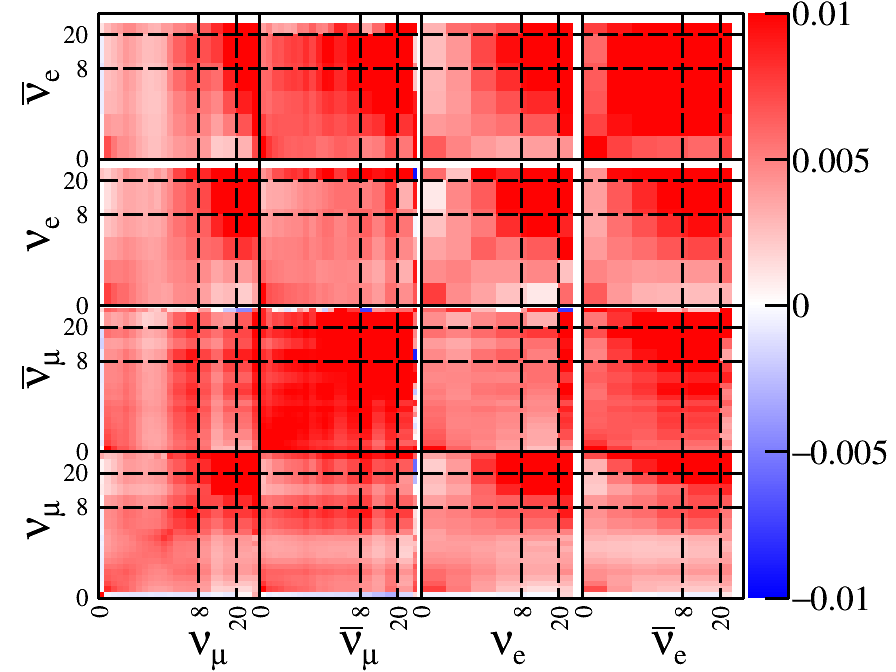
\includegraphics[width=0.45\textwidth]{graphics/FHC_LAR_nominal_cov_nom.png}}
  \subfloat[FHC post-fit] {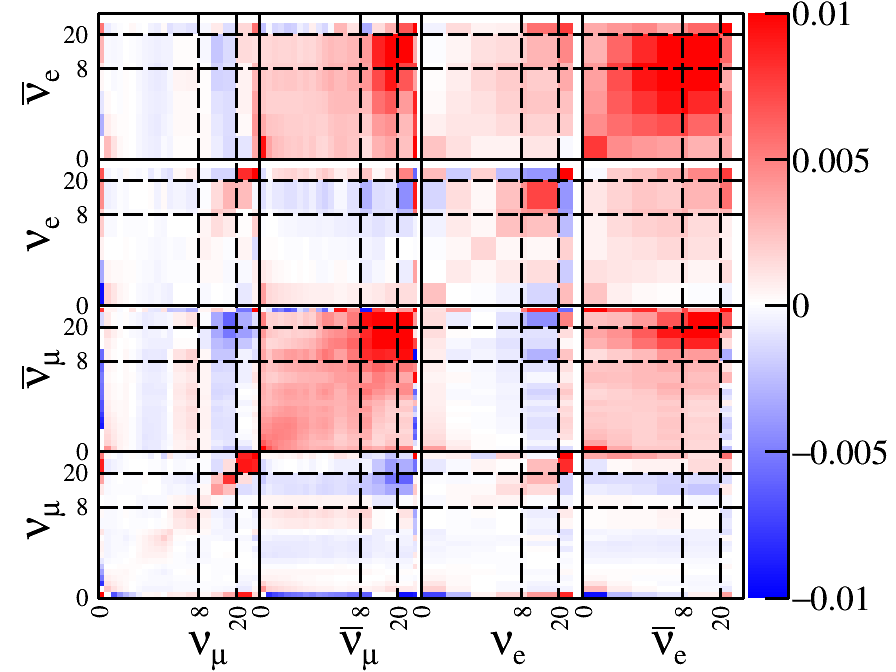
\includegraphics[width=0.45\textwidth]{graphics/FHC_LAR_nominal_cov_post.png}}
  \caption{Pre- and post-fit \dword{fhc} flux covariance matrices for the nominal \SI{35}{t} \dword{arcube} \dword{lar} detector using a five-year exposure.}
  \label{fig:LAR_nominal_covariances}
\end{figure}
The impact of the neutrino-electron scattering constraint on the flux covariance is shown in Figure~\ref{fig:LAR_nominal_covariances} for \dword{fhc} and a five year exposure of the nominal \SI{35}{t} \dword{arcube} \dword{lar} detector (corresponding to $\sim$22k neutrino-electron events). It is clear that the overall uncertainty on the flux has decreased dramatically, although, as expected, an anticorrelated component has been introduced between flavors (as it is not possible to tell what flavor contributed to the signal on an event-by-event basis). Similar constraints are obtained for \dword{rhc} running.

\begin{figure}[htbp]
  \centering
  \subfloat[Rate+shape]  {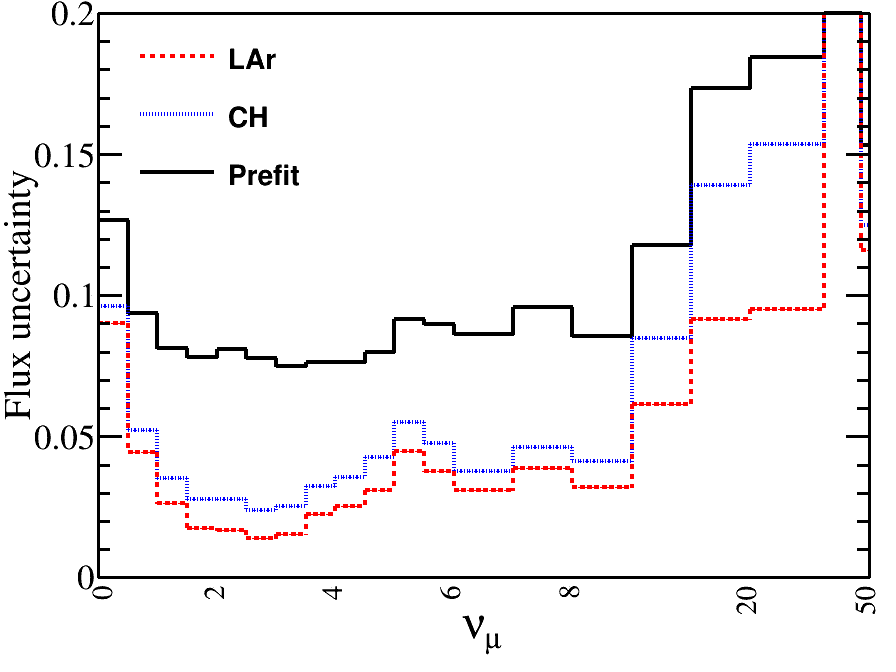
\includegraphics[width=0.45\textwidth]{graphics/FHC_DET_nominal_constraint_numu.png}}
  \subfloat[Shape-only]  {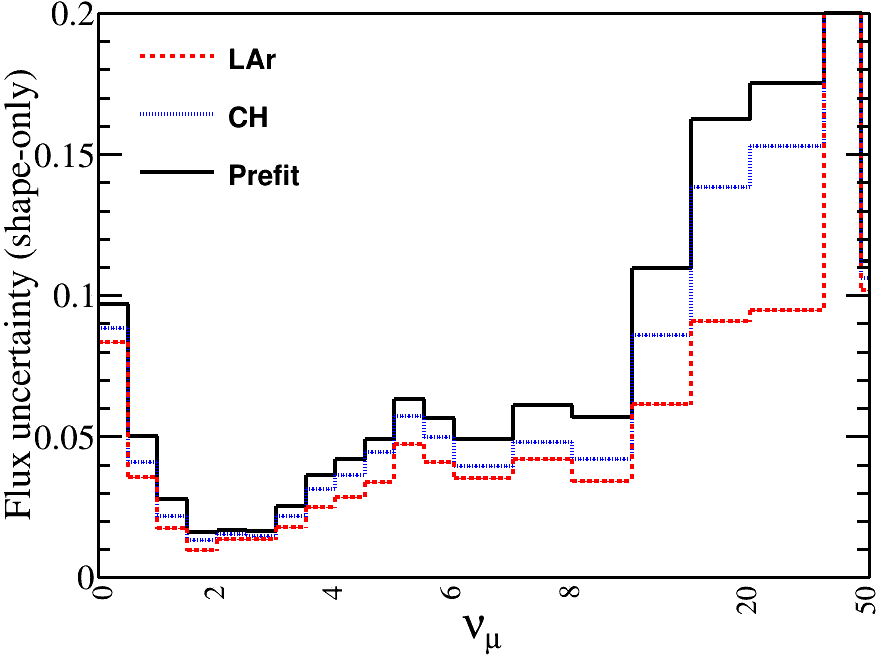
\includegraphics[width=0.45\textwidth]{graphics/FHC_DET_nominal_constraint_SHAPE_numu.png}}
  \caption{Rate+shape and shape-only bin-by-bin flux uncertainties as a function of neutrino energy for a 5 year exposure with various detector options, compared with the input flux covariance matrix before constraint.}
  \label{fig:nominal_det_constraint}
\end{figure}
Figure~\ref{fig:nominal_det_constraint} shows the flux uncertainty as a function of $E_{\nu}$ for the $\nu_{\mu}$-\dword{fhc} flux, for a variety of \dword{nd} options. In each case, the constraint on the full covariance matrix is calculated (as in Figure~\ref{fig:LAR_nominal_covariances}), but only the diagonal of the $\nu_{\mu}$ portion is shown. In the flux peak of $\sim$2.5 GeV, the total flux uncertainty can be constrained to $\sim$2\% for the nominal \dword{lar} scenario, and the constraint from other detector types is largely dictated by the detector mass. Clearly the neutrino electron scattering sample at the \dword{dune} \dword{nd} will be a powerful flux constraint. However, it is also clear that the ability to constrain the shape of the flux is not a drastic improvement on the existing flux covariance matrix, and none of the possible detectors investigated added a significantly stronger constraint. That said, the neutrino-electron sample is able to make \textit{in situ} measurements of the flux prediction, and is able to diagnose problems with the flux prediction in a unique way.


	


%%%%%%%%%%%%%%%%%%%%%%%%%%%%%%%%%%%%%%%%%%%%%%%%%%%%%%%%%%%%%%
\section{Multi-Purpose Detector}
\label{sec:exsum-nd-mpt}
%% \chapter defined in lbne-sci-opp-main.tex

The DUNE near neutrino detector provides scientific value beyond
      its essential role of calibrating beam and neutrino interaction
      properties for the long-baseline physics program described in
      Chapter~\ref{nu-oscil-chap}.
      By virtue of the theoretically clean, purely weak leptonic
      processes involved,
      neutrino beams have historically served as unique probes for
      new physics in their interactions with matter.
      The high intensity and broad energy range of the LBNF beam
      will open the door for a highly capable near detector
      to perform its own diverse
program of incisive investigations. 

%\fixme{Simplified this pgraph a bit per Jim's wish to make the ND seem less optional}
The reduction of systematic uncertainties for the neutrino oscillation
program %of the full DUNE scope requires a highly capable near neutrino detector (ND) to provide 
requires excellent resolution in the
reconstruction of neutrino events. Combined with the unprecedented
neutrino fluxes available %for the DUNE program 
--- which will
allow the collection of ${\cal{O}}$(\num{e8}) inclusive neutrino charged
current (CC) interactions for %\SI{e22}{\POT} 
\num{e22} protons-on-target (POT) just downstream of the
beamline --- the %inclusion of a 
near detector (ND)  %offers a unique opportunity to 
will significantly enhance the DUNE long-baseline 
oscillation program and produce a range of short-baseline neutrino
scattering physics measurements.  The combined statistics and
resolution expected in the ND will allow precise tests of fundamental
interactions resulting in a better understanding of the structure of
matter. 
Table~\ref{tab:rates} lists the expected number of %muon neutrino
beam-neutrino interactions per ton of detector at the DUNE ND site,
located \SI{459}{\meter} downstream from
the %beginning of the decay pipe
target.  
% \fixme{check this sentence; and the table 7.1 caption says
% 'interactions in the beams' (which is weird) and is for a water
% detector. Is this what you want?}  MB: interactions in the neutrino
% beam are interactions in the near detector when the neutrino beam is
% shining on it.  the calculations were made for water. leave as is
This chapter presents a short description of some of the studies that
can be performed with DUNE's fine-grained near neutrino detector
and gives a flavor of the outstanding physics potential. A more
detailed and complete discussion of the ND physics
potential can be found in~\cite{docdb-6704}.
Appendix~\ref{app-dis} describes neutrino scattering 
kinematics and includes
definitions of the kinematic variables used in this chapter.
\begin{table}[!htb]
\centering
\caption[Interaction rates, $\nu$ mode, per ton
for \SI{1e20}{\POT}, \SI{459}{\meter}, \SI{120}{\GeV}]{Estimated interaction rates in the neutrino (second column) and antineutrino (third column) beams per ton of detector (water) 
  for \SI{1e20}{\POT} at \SI{459}{\meter} assuming neutrino
  cross-section predictions from NUANCE~\cite{Casper:2002sd} and a \GeVadj{120}
  proton beam using the CDR reference design.  Processes are defined at the initial neutrino
  interaction vertex and thus do not include final-state effects. These estimates do not
  include detector efficiencies or acceptance~\cite{DOCDB740,DOCDB783}. 
}
\label{tab:rates}
\begin{tabular}[!htbp]{$L^r^r}%rl}  %$
\toprule
\rowtitlestyle
Production mode & $\nu_\mu$ Events & $\overline\nu_\mu$ Events\\
\toprowrule
CC QE ($\nu_\mu n \rightarrow \mu^- p$)                             & 50,100 & 26,300 \\ \colhline
NC elastic ($\nu_\mu N \rightarrow \nu_\mu N$)                      & 18,800 & 8,980 \\ \colhline
CC resonant $\pi^+$ ($\nu_\mu N \rightarrow \mu^- N \pi^+$)         & 67,800 & 0 \\ \colhline
CC resonant $\pi^-$ ($\overline{\nu}_\mu N \rightarrow \mu^+ N \pi^-$)   & 0      & 20,760 \\ \colhline
CC resonant $\pi^0$ ($\nu_\mu n \rightarrow \mu^- \ p \, \pi^0$)    & 16,200 & 6,700 \\ \colhline
NC resonant $\pi^0$ ($\nu_\mu N \rightarrow \nu_\mu \, N \, \pi^0$) & 16,300 & 7,130 \\ \colhline
NC resonant $\pi^+$ ($\nu_\mu p \rightarrow \nu_\mu \, n \, \pi^+$) & 6,930  & 3,200 \\ \colhline
NC resonant $\pi^-$ ($\nu_\mu n \rightarrow \nu_\mu \, p \, \pi^-$) & 5,980  & 2,570 \\ \colhline
CC DIS ($\nu_\mu N \rightarrow \mu^- X$ or 
$\overline{\nu}_\mu N \rightarrow \mu^+ X$, $W>2$)                     & 66,800 & 13,470 \\ \colhline
NC DIS ($\nu_\mu N \rightarrow \nu_\mu X$ or 
$\overline{\nu}_\mu N \rightarrow \overline{\nu}_\mu X$, $W>2$)                   & 24,100 & 5,560 \\ \colhline
NC coherent $\pi^0$ ($\nu_\mu A \rightarrow \nu_\mu A \pi^0$ or 
$\overline{\nu}_\mu A \rightarrow \overline{\nu}_\mu A \pi^0$
)       & 2,040  & 1,530 \\
CC coherent $\pi^+$ ($\nu_\mu A \rightarrow \mu^- A \pi^+$)         & 3,920  &  0 \\ \colhline
CC coherent $\pi^-$ ($\overline{\nu}_\mu A \rightarrow \mu^+ A \pi^-$)   & 0      & 2,900 \\ \colhline
NC resonant radiative decay ($N^* \rightarrow N \gamma $)          & 110    & 50 \\ \colhline
%Cabbibo-suppressed QE hyperon production & & \\ \colhline
%($\mu^+ \Lambda, \mu^+ \Sigma^0, \mu^+ \Sigma^-$) & 0 & xxx  \\ \colhline
NC elastic electron ($\nu_\mu e^- \rightarrow \nu_\mu e^-$  
or  $\overline{\nu}_\mu e^- \rightarrow \overline{\nu_\mu} e^-$)              & 30  & 17 \\ \colhline
Inverse Muon Decay ($\nu_\mu e \rightarrow \mu^- \nu_e$)            & 12  & 0\\ \colhline
Other                                                              & 42,600 & 15,800 \\ 
\toprule
\rowtitlestyle
Total CC  (rounded)                                                       & 236,000 & 81,000 \\ %81,340 \\
\rowtitlestyle
Total NC+CC  (rounded)                                                      & 322,000 & 115,000 \\%114,980 \\ 
\bottomrule
\end{tabular}
\end{table}
%%%%%%%%%%%%%%%%%%%%%%%%%%%%%%%%%%%%%%%%%%%%%%%%%%%%%%%%%%%%%%%%%%%%
\section{Precision Measurements with Long-Baseline Oscillations}
\label{sec-fluxosc}
From the studies of uncertainties and the impact of the spectral shape
presented in Section~\ref{sec:systs}, it is evident that to fully
realize the goals of the full DUNE scientific program --- in
particular, sensitivity to CP violation and the precision measurement
of the three-flavor oscillation parameters --- it is necessary to
characterize the expected unoscillated neutrino flux with high
precision. In addition to the precise determination of the neutrino
flux, shape and flavor composition, the characterization of different
neutrino interactions and interaction cross sections on a liquid argon target
is necessary to estimate physics backgrounds to the oscillation
measurements.  The high-resolution near tracking detector %such as that
described in Section~\ref{sec:ndproj} can measure the unoscillated flux
normalization, shape and flavor to a few percent using systematically
independent techniques that are %listed here and 
discussed in the following sections.
%%%%%%%%%%%%%%%%%%%%%%%%%%%%%%%%%%%%%%
\subsection{Determination of the Relative Neutrino and Antineutrino Flux} 
\label{sec-lownu0}
The most promising method of determining the shape of the \numu and
\anumu flux is by measuring CC events with low 
hadronic-energy deposition (low-$\nu$) where $\nu$ is the total energy of the
hadrons that are produced after a neutrino interaction, $E_\nu -
E_\mu$. It is important to note that not all the hadrons escape the
remnant nucleus, and intranuclear effects will smear the visible energy
of the hadronic system.  A method of relative flux determination known
as low-$\nu_0$ --- where $\nu_0$ is a given value of visible hadronic
energy in the interaction that is selected to minimize the fraction of
the total interaction energy carried by the hadronic system
--- is well developed~\cite{srmishra-reviewtalk}.  The method follows
from the general expression of the $\nu$-nucleon differential cross
section:
\begin{equation}
{\cal N} (\nu < \nu_0) \simeq C \Phi(E_\nu) \nu_0 \left[ {\cal A} +
\left( \frac{\nu_0}{E_\nu} \right) {\cal B} + \left( \frac{\nu_0}{E_\nu} \right)^2 {\cal C} +
{\cal O} \left( \frac{\nu_0}{E_\nu} \right)^3 \right],
\end{equation}
\noindent
where the coefficients are ${\cal A} = {\cal F}_2$, ${\cal B} = ({\cal
  F}_2 \pm {\cal F}_3)/2$, ${\cal C} = ({\cal F}_2 \mp {\cal F}_3)/6$, 
and ${\cal F}_i =\int^1_0 \int^{\nu_0}_0 F_i(x) dx d\nu$ is the
integral of structure function $F_i(x)$.  
%
The dynamics of
neutrino-nucleon scattering  implies that the number of events in a
given energy bin with hadronic energy $E_{\rm had} < \nu_0$ is
proportional to the (anti)neutrino flux in that energy bin up
to corrections ${\cal O}(\nu_0/E_\nu)$ and ${\cal O}(\nu_0/E_\nu)^2$.
%
The number ${\cal
  N}(\nu<\nu_0)$ is therefore proportional to the flux up to correction factors
of the order ${\cal O} (\nu_0/E_\nu)$ or smaller, which are not
significant for small values of $\nu_0$ at energies $\geq \nu_0$. 
 The coefficients ${\cal A}$, ${\cal B}$ and ${\cal C}$ are
determined for each energy bin and neutrino flavor within the ND data.
DUNE's primary interest is the relative flux
determination, i.e., the neutrino flux in one energy bin relative to that in
another; variations in the coefficients do not affect the
relative flux. The prescription for the relative flux determination is
simple: count the number of %$\nu$ 
neutrino CC events below a certain small
value of hadronic energy ($\nu_0$).  The observed number of events, up
to the correction of the order ${\cal O} (\nu_0/E_\nu)$ due to the
finite $\nu_0$ in each total visible energy bin, is proportional to
the relative flux. The smaller the factor $\nu_0/E_\nu$ is, the smaller
is the correction.  Furthermore, the energy of events passing the
low-$\nu_0$ cut is dominated by the corresponding lepton energy. 
It is
apparent from the above discussion that this method of relative flux
determination is not very sensitive to nucleon structure, QCD
corrections or types of neutrino interactions such as scaling or
nonscaling. With the excellent granularity and resolution foreseen in
the low-density magnetized tracker, it will be possible to use a value
of $\nu_0\sim$\SI{0.5}{\GeV} or lower, thus allowing flux predictions down to
$E_\nu \sim$\SI{0.5}{\GeV}. A preliminary analysis with the high-resolution
tracker achieved a precision $\leq 2\%$ on the relative $\nu_\mu$
flux with the low-$\nu_0$ method in the energy region $1 \leq E_\nu
\leq 30$ \si{GeV} in the fit with $\nu_0 < 0.5$ \si{\GeV}. Similar uncertainties
are expected for the $\overline{\nu}_\mu$ component (the dominant one) in
the antineutrino beam mode (negative focusing).
%%%%%%%%%%%%%%%%%%%%%%%%%%%%%%%%%%%%%%
\subsection{Determination of the Flavor Content of the Beam} 
%$\boldsymbol{\nu_\mu, \overline{\nu}_\mu, \nu_e, \overline{\nu}_e}$}
$\boldsymbol{\numu,\anumu, \nue, \anue}$
\fixme{I can't get this to compile with it in the heading. Anne}
The empirical parameterization %(EP)
of the pion and kaon neutrino parents produced from the proton target,
determined from the low-$\nu_0$ flux at the ND, allows prediction of
the $\nu_\mu$ and $\overline{\nu}_\mu$ flux at the far detector
location.  This parameterization provides a measure of the
$\pi^+/K^+/\mu^+(\pi^-/K^-/\mu^-)$ distributions of neutrino parents
of the beam observed in the ND.  Additionally, with the capability to
identify $\overline{\nu}_e$ CC interactions, it is possible to
directly extract the elusive $K^0_L$ content of the beam.  Therefore,
an accurate measurement of the $\nu_\mu, \overline{\nu}_\mu$ and
$\overline{\nu}_e$ CC interactions provides a prediction of the
$\nu_e$ content of the beam, which is an irreducible background for
the $\nu_e$ appearance search in the far detector:
\begin{eqnarray} \label{eqn:nueparents}
\nu_e & \equiv & \mu^+(\pi^+\to \nu_\mu) \oplus K^+(K^+\to \nu_\mu) \oplus K^0_L\\
\overline{\nu}_e & \equiv & \mu^-(\pi^-\to \overline{\nu}_\mu) \oplus K^-(K^-\to \overline{\nu}_\mu) \oplus K^0_L
\end{eqnarray}
The $\mu$ component is well constrained from $\nu_\mu
(\overline{\nu}_\mu)$ CC data at low energy, while the $K^\pm$
component is only partially constrained by the $\nu_\mu
(\overline{\nu}_\mu)$ CC data at high energy and requires external
hadro-production measurements of $K^\pm/\pi^\pm$ ratios at low energy
from hadro-production experiments such as MIPP~\cite{Raja:2005sh} and
NA61~\cite{Korzenev:2013gia}.  Finally, the $K_L^0$ component can be
constrained by the $\overline{\nu}_e$ CC data and by external
dedicated measurements at hadron-production experiments.  In the
energy range $1 (5) \leq E_\nu \leq 5 (15)$ \si{GeV}, the approximate
relative contributions to the $\nu_e$ spectrum are 85\% (55\%) from
$\mu^+$, 10\% (30\%) from $K^+$ and 3\% (15\%) from $K_L^0$.
Based on the NOMAD experience, %we expect to achieve
a precision of $\leq 0.1\%$ on the flux ratio $\nu_e/\nu_\mu$ is
expected at high energies. Taking into account the projected precision
of the $\nu_\mu$ flux discussed in Section~\ref{sec-lownu0}, this
translates into an absolute prediction for the $\nu_e$ flux at the
level of $2\%$.
Finally, the fine-grained ND can directly identify $\nu_e$ CC
interactions from the LBNF beam. The relevance of this measurement is
twofold:
\begin{enumerate}
\item It provides an independent
validation for the flux predictions obtained from the low-$\nu_0$ method.
\item It can
further constrain the uncertainty on the knowledge of the absolute $\nu_e$ flux.
\end{enumerate}
%%%%%%%%%%%%%%%%%%%%%%%%%%%%%%%%%%%%%%
\subsection{Constraining the Unoscillated $\nu$ %$\boldsymbol{\nu}$ 
Spectral Shape with the QE Interaction}
\fixme{took out bold -won't compile. Anne}

In any long-baseline neutrino oscillation program, including DUNE, the
quasi-elastic (QE) interactions are special.  First, the QE cross
section is substantial at lower energies~\cite{Formaggio:2013kya}.
Second, because of the simple topology (a $\mu^-$ and a proton), the
visible interaction energy provides, to first order, a close
approximation to the neutrino energy ($E_\nu$).  
In the context of a fine-grained tracker, a precise measurement of QE
will impose direct constraints on nuclear effects related to both the
primary and final-state interaction (FSI) dynamics 
(Section~\ref{sec-nuclear}), which can affect the overall neutrino
energy scale and, thus, the entire oscillation program.  To this end,
the key to reconstructing a high-quality sample of $\nu_\mu$ QE
interactions is the two-track topology where both final-state
particles are visible: $\mu^-$ and $p$. A high-resolution ND can
efficiently identify the recoil proton and measure its momentum vector
as well as $dE/dx$. Preliminary studies indicate that in a
fine-grained tracking detector the efficiency (purity) for the proton
reconstruction in QE events is $52\%$ ($82\%$). A comparison between
the neutrino energy reconstructed from the muon momentum through the
QE kinematics (assuming a free target nucleon) with the visible
neutrino energy measured as the sum of $\mu$ and $p$ energies is
sensitive to both nuclear effects and FSI. Furthermore, comparing the
two-track sample ($\mu$ and $p$) with the single-track sample (in which only $\mu$
is reconstructed) empirically constrains the rate of FSI.
%%%%%%%%%%%%%%%%%%%%%%%%%%%%%%%%%%%%%%
\subsection{Low-Energy Absolute Flux: Neutrino-Electron NC Scattering}
\label{ssec:ncscatter}
Neutrino neutral current (NC) interaction with the atomic electron in the
target, $\nu_\mu e^- \rightarrow \nu_\mu e^-$, provides an elegant
measure of the absolute flux.  The total cross section for NC elastic
scattering off electrons is given by~\cite{Marciano:2003eq}:
\begin{eqnarray}
\sigma (\nu_l e \to \nu_l e) & = & \frac{G_\mu^2 m_e E_\nu}{2\pi} \left[ 1 -4 \sin^2 \theta_W + \frac{16}{3} \sin^4 \theta_W \right], \\
\sigma (\overline{\nu}_l e \to \overline{\nu}_l e) & = & \frac{G_\mu^2 m_e E_\nu}{2\pi} \left[ \frac{1}{3} -\frac{4}{3} \sin^2 \theta_W + \frac{16}{3} \sin^4 \theta_W \right], 
\end{eqnarray}
\noindent
where $\theta_W$ is the weak mixing angle (WMA).  For the currently
known value of $\sin^2 \theta_W\simeq0.23$, the above cross sections
are very small: $\sim 10^{-42} (E_\nu/{\rm GeV})$~cm$^2$. The NC
elastic scattering off electrons can be used to determine the absolute
flux normalization since the cross section only depends on the
knowledge of $\sin^2 \theta_W$. Within the Standard Model, the value
of $\sin^2 \theta_W$ at the average momentum transfer expected at
DUNE, $Q\sim0.07$~\si{\GeV}, can be extrapolated down from the
LEP/SLC\footnote{LEP was the Large Electron-Positron Collider at CERN
  that operated from 1989 to 2000 and provided a detailed study of the
  electroweak interaction.}  measurements with a precision of $\leq
1\%$. The \numu $e^- \rightarrow$ \numu $e^-$ will produce a single
$e^-$ collinear with the $\nu$-beam ($\leq 40$~mrad).  The background,
dominated by the asymmetric conversion of a photon in an ordinary
$\nu$-nucleon NC event, will produce $e^-$ and $e^+$ in equal measure
with much broader angular distribution.  A preliminary analysis of the
expected elastic scattering signal in the high-resolution tracking ND
shows that the scattering signal can be selected with an efficiency of
about 60\% with a small background contaminant. The measurement will
be dominated by the statistical error. %We estimate that
The determination of the absolute flux of the DUNE neutrinos is
estimated to reach a precision of $\simeq 2.5\%$ for $E_\nu \leq
10$~\si{\GeV}.  The measurement of NC elastic scattering off electrons
can only provide the integral of all neutrino flavors.
%%%%%%%%%%%%%%%%%%%%%%%%%%%%%%%%%%%%%%
\subsection{High-Energy Absolute Flux: Neutrino-Electron CC Scattering}
The \numu-$e^-$ CC interaction, \numu$ + e^- \rightarrow \mu^- +
$\nue (\emph{inverse muon decay} or \emph{IMD}), offers an elegant
way to determine the absolute flux. Given the energy threshold needed
for this process, IMD requires %a minimum
$E_\nu \geq 10.8$~\si{\GeV}.  The high-resolution ND in the
LBNF beam will observe $\geq$ \num{2000} IMD events in three
years. The reconstruction efficiency of the single, energetic %and
forward $\mu^-$ will be $\geq$ 98\%; the angular resolution of the
IMD $\mu$ is $\leq$ \SI{1}{\mrad}. The background, primarily from the
$\nu_\mu$-QE interactions, can be precisely constrained using control
samples.  In particular, the systematic limitations of the CCFR
(\cite{Mishra:1989jn,Mishra:1990yf}) and %those of
the CHARM-II~\cite{Vilain:1996yf} IMD measurements can be
substantially alleviated in DUNE with the proposed ND design. A
preliminary analysis indicates that the absolute flux can be
determined with an accuracy of $\approx 3\%$ for $E_\nu \geq$
\SI{11}{\GeV} (average $E_\nu \approx$\SI{25}{\GeV}).
%%%%%%%%%%%%%%%%%%%%%%%%%%%%%%%%%%%%%%
\subsection{Low-Energy Absolute Flux: QE in Water and Heavy-Water Targets}
Another  % third 
independent method to extract the absolute flux is through the
QE-CC scattering ($\nu_\mu n(p) \to \mu^- p(n)$) on
deuterium at low $Q^2$. Neglecting terms in $(m_\mu/M_n)^2$ at $Q^2=0$,
the QE cross section is independent of neutrino energy for $(2E_\nu
M_n)^{1/2} > m_\mu$:
\begin{equation}
\frac{d \sigma}{d Q^2}  \mid {Q^2=0}\mid = \frac{G_\mu^2 \cos^2 \theta_c}{2\pi}
\left[ F_1^2(0) + G_A^2(0) \right] = 2.08 \times 10^{-38}~\rm cm^2{\rm GeV}^{-2},
\end{equation}
%
\noindent 
which is determined by neutron $\beta$ decay and has a theoretical
uncertainty $<1\%$.  The flux can be extracted experimentally by
measuring low $Q^2$ QE interactions ($ \leq 0.05$ GeV) and extrapolating
the result to the limit of $Q^2=0$. The measurement requires a
deuterium (or hydrogen for antineutrino) target to minimize the
smearing due to Fermi motion and other nuclear effects. This
requirement can only be achieved by using both H$_2$O and D$_2$O
targets embedded in the fine-grained tracker and extracting the events
produced in deuterium by statistical subtraction of the larger oxygen
component.  The experimental resolution on the muon and proton
momentum and angle is crucial.  Dominant uncertainties of the method
are related to the extrapolation to $Q^2=0$, to the theoretical cross
section on deuterium, to the experimental resolution and to the
statistical subtraction.  Sensitivity studies and the experimental
requirements are under study.
%%%%%%%%%%%%%%%%%%%%%%%%%%%%%%%%%%%%%%
%\subsection{Neutral Pions, Photons and $\boldsymbol{\pi^{\pm}}$ in NC and CC Events}
\subsection{Neutral Pions, Photons and $\pi^{\pm}$ in NC and CC Events}
\fixme{removed bold. Anne}

\label{sec-bkgnds}
The principal background to the $\nu_e$ and $\overline{\nu}_e$
appearance comes from the NC events where a photon from the $\pi^0$
decay produces a signature similar to that produced by $\nu_e$-induced
electron; the second source of background is due to $\pi^0$'s from
$\nu_\mu$ CC where the $\mu^-$ evades identification --- typically at
high $y_{Bj}$.  Since the energy spectra of NC and CC interactions are
different, it is critical for the ND to measure $\pi^0$'s in NC and CC
interactions in the full kinematic phase space.
 
The proposed ND is designed to measure $\pi^0$'s with 
high accuracy in three topologies: 
\begin{enumerate}
\item Both photons convert 
in the tracker ($\simeq$25\%).
\item One photon converts  
in the tracker and the other in the calorimeter ($\simeq$50\%). 
\item Both photons convert in the calorimeter;  
the first two topologies afford the best resolution 
because the tracker provides precise $\gamma$-direction measurement. 
\end{enumerate}
The $\pi^0$ reconstruction efficiency in the proposed fine-grained tracker is
expected to be $\geq$75\% if photons that reach the ECAL are
included.   By contrasting the $\pi^0$ mass  in the tracker
versus in the calorimeter, the relative efficiencies 
of photon reconstruction will be well constrained. 
Finally, the $\pi^{\pm}$ track momentum and $dE/dx$ information will
be measured by the tracker.  An in situ determination of the charged
pions in the $\nu_{\mu}/\overline{\nu}_\mu$ CC events --- with $\mu$ID and
without $\mu$ID --- and in the $\nu$ NC events is crucial to constrain
the systematic error associated with the \numu (\anumu) disappearance,
especially at low $E_\nu$.
%%%%%%%%%%%%%%%%%%%%%%%%%%%%%%%%%%%%%%
\subsection{Signal and Background Predictions for the Far Detector} 
\label{sec-extfd} 
In order to achieve reliable predictions for signal and backgrounds in the far detector, near detector measurements --- including (anti)neutrino fluxes, nuclear cross sections and detector 
smearing --- must be unfolded and extrapolated to the far detector location. 
The geometry of the beam and detectors (point source versus extended source) 
as well as the expected neutrino oscillations imply differences in the (anti)neutrino fluxes 
 in the near and far detectors. 
These differences, in turn, will result in increased sensitivity of the long-baseline analysis to cross-section uncertainties, in particular between neutrinos and antineutrinos and for exclusive background topologies. 
Furthermore, the much higher event rates at the near site and the 
smaller detector size (i.e., reduced containment) make it virtually impossible to achieve identical measurement 
conditions in both the near and far detectors. However, as discussed in 
Sections~\ref{sec-lownu0} to~\ref{sec-bkgnds}, the energy, angular and 
space resolution of the low-density %, fine-grained (AH: seems like too much advertisement)
ND are key factors in reducing the systematic uncertainties achievable 
on the event predictions for the far detector; the ND can offer a precise \emph{in situ} 
measurement of the absolute flux of all flavor components of the beam, 
$\nu_\mu, \nu_e, \bar\nu_\mu, \bar \nu_e$, resulting in constraints on the parent 
$\pi^\pm/K^\pm/\mu^\pm$ distributions. 
%
In addition, measurements of momenta and energies of final-state particles produced 
in (anti)neutrino interactions will allow a detailed study of exclusive topologies affecting the 
signal and background rates in the far detector. 
All of these measurements will be used to cross-check and fine-tune the simulation programs  
needed for the actual extrapolation from the near to the far detector. 
It is important to note that several of these techniques have already been used and \emph{proven to work} 
in neutrino experiments such as MINOS~\cite{Adamson:2009ju} and 
NOMAD~\cite{Wu:2007ab,Lyubushkin:2008pe,Samoylov:2013xoa}. 
The higher segmentation and resolution in the DUNE ND with respect to past experiments 
will increase the available information about the (anti)neutrino event topologies, allowing further 
reduction of systematic uncertainties both in the ND measurements and in the Monte Carlo extrapolation.  
For a more detailed discussion of the impact of ND measurements on the long-baseline oscillation analysis see 
Section~\ref{sec:systs}.  
 
\clearpage
%%%%%%%%%%%%%%%%%%%%%%%%%%%%%%%%%%%%%%%%%%%%%%%
\section{Electroweak Precision Measurements} 
\label{sec-ew-wma}

  Neutrinos and antineutrinos are the most effective probes for
  investigating electroweak physics.  Interest in a precise
  determination of the weak mixing angle ($\sin^2 \theta_W$) at DUNE
  energies via neutrino scattering is twofold: (1) it provides a
  direct measurement of neutrino couplings to the $Z$ boson and (2) it
  probes a different scale of momentum transfer than LEP 
did by virtue of not being at the $Z$ boson mass peak. 

The weak mixing angle can be extracted
experimentally from three main NC physics processes:
\begin{enumerate}%[parsep=-1pt]
%\item Deep Inelastic Scattering off quarks inside nucleons: $\nu N \to \nu X$ ($W>2$~GeV)
\item deep inelastic scattering off quarks inside nucleons: $\nu N \to \nu X$
\item elastic scattering off electrons: $\nu e^- \to \nu e^-$
\item elastic scattering off protons: $\nu p \to \nu p$
\end{enumerate}

%Figure~\ref{fig:graphs} shows the Feynman diagrams corresponding to the three processes.
%
%\begin{figure}[!htb]
%\centering
%  \feynmanNC{$\nu$}{neutrino}{$q,\overline{q}$}{quark}{0.3\linewidth}
%  \feynmanNC{$\nu$}{neutrino}{$e^-$}{lepton}{0.3\linewidth}
%  \feynmanNC{$\nu$}{neutrino}{$N$}{hadron}{0.3\linewidth}
%  
%  \caption[Feynman diagrams for the three main NC
%  processes]{Feynman diagrams for the three main neutral current
%    processes that can be used to extract $\sin^2 \theta_W$ with the
%    DUNE near detector.  From left, deep inelastic scattering off
%    quarks, elastic scattering off electrons and elastic scattering
%    off nucleons.  }
%\label{fig:graphs}
%\end{figure}

%%%%%%%%%%%%%%%%%%%%%%%%%%%%%%%%%%%%%%
\subsection{Deep Inelastic Scattering} 
\label{ssec:nd:dis}
The most precise measurement of $\sin^2 \theta_W$ in
neutrino deep inelastic scattering (DIS) comes from the NuTeV experiment, which reported
a value that is $3\sigma$ from the Standard Model~\cite{Zeller:2001hh}. 
The DUNE ND can perform a similar
analysis in the DIS channel by measuring the ratio of NC and CC interactions induced by
neutrinos:
\begin{equation}
{\cal R}^\nu \equiv \frac{\sigma^\nu_{\rm NC}}{\sigma^\nu_{\rm CC}}
 \simeq \rho^2 \left( \frac{1}{2} - \sin^2 \theta_W +\frac{5}{9} \left(1 + r \right) \sin^4 \theta_W  \right).
\end{equation}
\noindent
Here $\rho$ is the relative coupling strength of the
neutral-to-charged current interactions ($\rho =1$ at tree-level in
the Standard Model) and $r$ is the ratio of antineutrino to neutrino
cross section ($r\sim0.5$).  The absolute sensitivity of ${\cal
  R}^\nu$ to $\sin^2 \theta_W$ is 0.7, which implies that a
measurement of ${\cal R}^\nu$ to 1\% precision would in turn provide a
1.4\% precision on $\sin^2 \theta_W$.  This technique was used by the
CDHS~\cite{Abramowicz:1986vi}, CHARM~\cite{Allaby:1987vr} and CCFR~\cite{Reutens:1985hv} 
experiments. In contrast to the NuTeV experiment, the antineutrino
interactions cannot be used for this analysis at DUNE due to the large
number of $\nu_\mu$ DIS interactions in the $\overline{\nu}_\mu$ beam
compared to the $\overline{\nu}_\mu$ DIS interactions.
The measurement of $\sin^2 \theta_W$ from DIS interactions can only be
performed with a low-density magnetized tracker since an accurate
reconstruction of the NC event kinematics and of the $\nu$ CC
interactions are crucial for keeping the systematic uncertainties on
the event selection under control. The analysis selects events in the
ND after imposing a cut on the visible hadronic energy of $E_{\rm had}
>$~\SI{5}{\GeV} (the CHARM analysis had $E_{\rm had} >$~\SI{4}{\GeV}).
With an exposure of $5\times 10^{21}$ POT in the \SIadj{120}{\GeV}
beam using the CDR reference design, about $7.7 \times 10^6$ CC events
and $2.4 \times 10^6$ NC events are expected, giving a statistical
precision of 0.074\% on ${\cal R}^\nu$ and 0.1\% on $\sin^2 \theta_W$
(Table~\ref{tab:NuTeV-sin2tw}).

\begin{dunetable}[Uncertainties on the ${\cal R}^\nu$ measurement]{llll}{tab:NuTeV-sin2tw}
{Comparison of uncertainties on the ${\cal R}^\nu$ measurement between NuTeV and DUNE with a 5 t fiducial mass after an exposure of $5\times 10^{21}$ POT (5 year) with the CDR reference \SIadj{120}{\GeV} beam. The corresponding relative uncertainties on $\sin^2 \theta_W$ must be multiplied by a factor of 1.4, giving for DUNE a projected overall precision of 0.35\%.}

Source of uncertainty & \multicolumn{2}{c}{~~~~~~~ $\delta R^{\nu}/R^{\nu}$~~~~~~~ } & 
Comments \\
& NuTeV & DUNE & \\ 
\toprowrule
 Data statistics & 0.00176 & 0.00074 & \\ \colhline
 Monte Carlo statistics & 0.00015   &  & \\ \colhline
 \textit{Total Statistics} &  \textit{0.00176} &  \textit{0.00074} & \\
 \midrule
$\nu_{e}, \overline{\nu}_{e}$ flux ($\sim1.7\%$) & 0.00064 &  0.00010 & 
$e^-/e^+$ identification \\ \colhline
 Energy measurement &  0.00038 &  0.00040 & \\ \colhline
 Shower length model &  0.00054 &  n.a. & \\ \colhline
 Counter efficiency, noise &  0.00036 &  n.a. & \\ \colhline
 Interaction vertex & 0.00056 &  n.a. & \\ \colhline
 $\overline{\nu}_\mu$ flux    &  n.a. &  0.00070 & Large $\bar \nu$ contamination \\ \colhline
 Kinematic selection    &  n.a. &  0.00060 & Kinematic identification of NC \\  \colhline
  \textit{Experimental systematics} &  \textit{0.00112} &   \textit{0.00102} & \\ 
\midrule 
 d,s$\rightarrow$c, s-sea &  0.00227 &  0.00140 & Based on existing knowledge \\ \colhline
 Charm sea &  0.00013  &   n.a. & \\
 $r = \sigma^{\overline{\nu}}/\sigma^{\nu}$ &  0.00018 &  n.a. & \\ \colhline
 Radiative corrections & 0.00013 &  0.00013 & \\ \colhline
 Non-isoscalar target &  0.00010 &  N.A. &  \\ \colhline
 Higher twists &  0.00031 &   0.00070 & Lower $Q^2$ values \\ \colhline
 $R_{L}$ ($F_2,F_T,xF_3$) &  0.00115 &   0.00140 & Lower $Q^2$ values \\ \colhline
 Nuclear correction    &        &  0.00020 &  \\  \colhline
  \textit{Model systematics} &   \textit{0.00258} &    \textit{0.00212} & \\ 
\toprule
\rowtitlestyle
 Total  &  0.00332 &     0.00247 &  \\
\bottomrule
\end{dunetable}
The use of a low-density magnetized tracker can substantially reduce
systematic uncertainties compared to a massive
calorimeter. Table~\ref{tab:NuTeV-sin2tw} shows a comparison of the
different uncertainties on the measured ${\cal R}^\nu$ between NuTeV
and DUNE.  While NuTeV measured both ${\cal R}^\nu$ and ${\cal
  R}^{\overline{\nu}}$, the largest experimental uncertainty in the
measurement of ${\cal R}^\nu$ is related to the subtraction of the
$\nu_e$ CC contamination from the NC sample. Since the low-density
tracker at DUNE can efficiently reconstruct the electron tracks, the
$\nu_e$ CC interactions can be identified on an event-by-event basis,
reducing the corresponding uncertainty to a negligible
level. Similarly, uncertainties related to the location of the
interaction vertex, noise, counter efficiency and so on are removed by
the higher resolution and by changing the analysis selection. The
experimental selection at DUNE will be dominated by two uncertainties:
the knowledge of the $\overline{\nu}_\mu$ flux and the kinematic
selection of NC interactions. The former is relevant due to the larger
NC/CC ratio for antineutrinos. The total experimental systematic
uncertainty on $\sin^2 \theta_W$ is expected to be about 0.14\%.
The measurement of ${\cal R}^\nu$ will be dominated by theoretical
systematic uncertainties on the structure functions of the
target nucleons.  The estimate of these uncertainties for DUNE is
based upon the extensive work performed for the NOMAD analysis and
includes a Next-to-Next-Leading-Order (NNLO) QCD calculation of
structure functions (NLO for charm
production)~\cite{Alekhin:2007fh,Alekhin:2008ua,Alekhin:2008mb},
parton distribution functions (PDFs) extracted from dedicated low-$Q$
global fits, high-twist contributions~\cite{Alekhin:2007fh},
electroweak corrections~\cite{Arbuzov:2004zr} and nuclear
corrections~\cite{Kulagin:2004ie,Kulagin:2007ju,Kulagin:2010gd}. The
charm quark production in CC, which has been the dominant source of
uncertainty in all past determinations of $\sin^2 \theta_W$ from
$\nu$N DIS, is reduced to about 4\% of the total $\nu_\mu$ CC DIS for
$E_{\rm had}>5$~GeV with the low-energy beam spectrum at DUNE.  This
number translates into a systematic uncertainty of 0.14\% on ${\cal
  R}^\nu$ (Table~\ref{tab:NuTeV-sin2tw}), assuming the current
knowledge of the charm production cross section.  It is worth noting
that the recent measurement of charm dimuon production by the NOMAD
experiment allowed a reduction of the uncertainty on the strange sea
distribution to $\sim3\%$ and on the charm quark mass $m_c$ to
$\sim75$~MeV~\cite{Samoylov:2013xoa}. The
lower neutrino energies available at DUNE reduce the accessible $Q^2$
values with respect to NuTeV, increasing in turn the effect of
non-perturbative contributions (high twists) and $R_L$. The
corresponding uncertainties are reduced by the recent studies of
low-$Q$ structure functions and by improved modeling with respect to
the NuTeV analysis (NNLO vs. LO).  The total model systematic
uncertainty on $\sin^2 \theta_W$ is expected to be about 0.21\% with
the reference beam configuration. The corresponding total uncertainty
on the value of $\sin^2 \theta_W$ extracted from $\nu$N DIS is 0.35\%.
Most of the model uncertainties will be constrained by dedicated in
situ measurements using the large CC samples and employing
improvements in theory that will have evolved over the course of the
experiment. The low-density tracker will collect about \num{350000}
neutrino-induced inclusive charm events in a five-year run with the
%reference 
\SIadj{120}{\GeV} \MWadj{1.2} beam.  The precise
reconstruction of charged tracks will allow measurement of exclusive
decay modes of charmed hadrons (e.g., $D^{*+}$) and measurement of
charm fragmentation and production parameters. The average
semileptonic branching ratio $B_\mu$ is of order $5\%$ with the
low-energy LBNF beam, and the low-density ND will be able to
reconstruct both the $\mu \mu$ and $\mu e$ decay channels. Currently,
the most precise sample of \num{15400} dimuon events has been
collected by the NOMAD experiment.  Finally, precision measurements of
CC structure functions in the DUNE ND would further reduce the
uncertainties on PDFs and on high-twist contributions.
The precision that can be achieved from $\nu$N DIS interactions is
limited by both the event rates and the energy spectrum of the
%reference \kWadj{700} beam configuration.  The high-statistics beam
standard beam configuration.  The high-statistics beam
exposure with the low-energy default beam-running configuration
(described in Chapter~\ref{project-chap}) combined with a dedicated
run with the high-energy beam option would increase the statistics by
more than a factor of ten. This major step forward would not only
reduce the statistical uncertainty to a negligible level, but would
provide large control samples and precision auxiliary measurements to
reduce the systematic uncertainties on structure functions. The two
dominant systematic uncertainties, charm production in CC interactions
and low $Q^2$ structure functions, are essentially defined by the
available data at present.  Overall, the use of a high-energy beam
with upgraded intensity can potentially improve the precision
achievable on $\sin^2 \theta_W$ from $\nu$N DIS to better than 0.2\%.  
%%%%%%%%%%%%%%%%%%%%%%%%%%%%%%%%%%%%%%
\subsection{Elastic Scattering} 
A second independent measurement of $\sin^2 \theta_W$ can be obtained
from NC $\nu_\mu e$ elastic scattering. This channel has lower
systematic uncertainties since it does not depend on knowledge of
the structure of nuclei, but it has limited statistics due to its very
low cross section. The value of $\sin^2 \theta_W$ can be extracted
from the ratio of interactions~\cite{Marciano:2003eq} as follows:
\begin{equation} \label{eqn:NCel}
{\cal R}_{\nu e} (Q^2) \equiv \frac{\sigma(\overline{\nu}_\mu e \to \overline{\nu}_\mu e)}{\sigma(\nu_\mu e \to \nu_\mu e)} (Q^2)
\simeq \frac{1 - 4 \sin^2 \theta_W + 16 \sin^4 \theta_W}{3 -12 \sin^2 \theta_W + 16 \sin^4 \theta_W},
\end{equation}
\noindent 
in which systematic uncertainties related to the selection and the
electron identification cancel out.  The absolute sensitivity of this
ratio to $\sin^2 \theta_W$ is 1.79, which implies that a measurement of
${\cal R}_{\nu e}$ to 1\% precision would provide a 
measurement of $\sin^2 \theta_W$ to 0.65\% precision.
The best measurement of NC elastic scattering off electrons was
performed by CHARM II, which observed 2677$\pm82$ $\nu$ and 2752$\pm$88
$\overline{\nu}$ events~\cite{Vilain:1994qy}. 
The CHARM II analysis was characterized by a
sizable uncertainty related to the extrapolation of the background
into the signal region.  
The event selection for NC elastic scattering is described in
Section~\ref{ssec:ncscatter}.  Since the NC elastic scattering off
electrons is also used for the absolute flux normalization, the WMA
analysis can be performed only with the low-density, magnetized tracker
in conjunction with a large liquid argon detector. In the case of the flux
normalization measurement, the total reconstructed statistics is
limited to about 4,500 (2,800) $\nu(\bar \nu)$ events.  These numbers
do not allow a competitive determination of $\sin^2 \theta_W$ by using
the magnetized tracker alone.  However, a \tonneadj{100} liquid argon detector
in the ND %complex,
would be expected to collect about 90,000 (60,000) reconstructed $\nu
(\overline{\nu})$ events with the standard beam, and an additional factor of two with 
an upgraded \MWadj{2.3} beam. 
A combined analysis of both detectors can achieve the optimal
sensitivity: the fine-grained tracker is used to reduce systematic
uncertainties (measurement of backgrounds and calibration), while the
liquid argon %near 
detector provides the statistics required for a competitive measurement.
Overall, the use of the complementary liquid argon detector can provide a statistical
accuracy on $\sin^2 \theta_W$ of about 0.3\%.  However, the extraction
of the WMA is dominated by the systematic uncertainty on the
$\overline{\nu}_\mu / \nu_\mu$ flux ratio in
Equation~(\ref{eqn:NCel}).  This uncertainty has been evaluated with
the low-$\nu_0$ method for the flux extraction and a systematic
uncertainty of about 1\% was obtained on the ratio of the
$\overline{\nu}_\mu / \nu_\mu$ flux integrals.  An improved precision
on this quantity could be achieved from a measurement of the
ratios $\pi^-/\pi^+$ and $\rho^-/\rho^+$ from coherent production in
the fine-grained tracker.  Due to the excellent angular and momentum
resolution and to large cancellations of systematic uncertainties,
preliminary studies indicate that an overall precision of about 0.3\% can
be achieved on the $\overline{\nu}_\mu / \nu_\mu$ flux ratio using
coherent production.
%Therefore, the overall precision on $\sin^2 \theta_W$ achievable from
%NC elastic scattering off electrons is limited to about 0.9\%. 
\begin{figure}[!htb]
\centering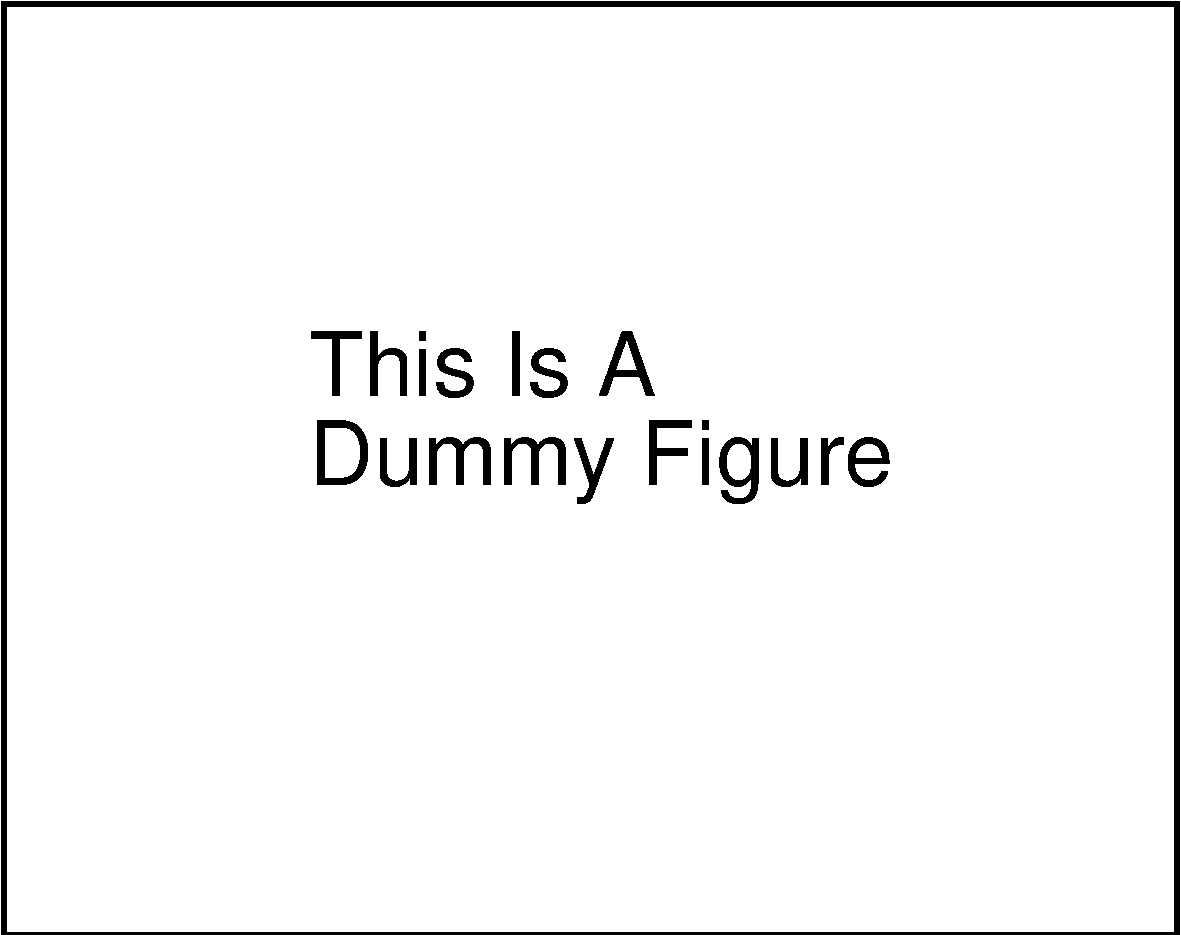
\includegraphics[width=.8\textwidth]{graphics/dummy.pdf}
%\vspace*{6.0cm}
\caption[Expected near detector sensitivity to $\sin^2 \theta_W$ 
for a \MWadj{1.2} beam]{Expected sensitivity to the measurement of $\sin^2 \theta_W$ from the DUNE ND
with the reference \MWadj{1.2} beam and an exposure of $5\times 10^{21}$ POT with a neutrino beam (five years) and 
$5\times 10^{21}$ POT with an antineutrino beam (five years). 
The curve shows the Standard Model prediction as a function of the 
momentum scale~\cite{Czarnecki:2000ic}.
Previous measurements from Atomic Parity Violation~\cite{Bennett:1999zza,Yao:2006px}, Moeller
scattering (E158~\cite{Anthony:2005pm}), $\nu$ DIS (NuTeV~\cite{Zeller:2001hh}) 
and the combined $Z$ pole  measurements (LEP/SLC)~\cite{Yao:2006px}  are also shown for comparison.
The use of a high-energy beam tune
can reduce the DUNE uncertainties by almost a factor of two.
%[figure to be finalized, space holder]
}
\label{fig:sin2thetaw}
\end{figure}
Together, the DIS and the NC elastic scattering channels involve
substantially different scales of momentum transfer, providing a tool
to test the running of $\sin^2 \theta_W$ in a single experiment. To
this end, the study of NC elastic scattering off protons can provide
additional information since it occurs at a momentum scale that is
intermediate between the two other processes.
% Furthermore, in the two NC elastic processes off electrons and
% protons it is possible to reconstruct the $Q^2$, providing
% additional sensitivity.
Figure~\ref{fig:sin2thetaw} summarizes the target sensitivity from the
DUNE ND, compared with existing measurements as a function of the
momentum scale.
In the near future, another precision measurement of $\sin^2 \theta_W$
is expected from the $Q_{\rm weak}$ experiment~\cite{Lee:2013kya}
at Jefferson Laboratory. From the
measurement of parity-violating asymmetry in elastic electron-proton
scattering, the $Q_{\rm weak}$ experiment should achieve a precision
of 0.3\% on $\sin^2 \theta_W$ at $Q^2=0.026$ GeV$^2$.  It should be
noted that the $Q_{\rm weak}$ measurement is complementary to those
from neutrino scattering given the different scale of momentum
transfer and the fact that neutrino measurements are the only direct
probe of the $Z$ coupling to neutrinos. With the \GeVadj{12} upgrade
of Jefferson Laboratory, the $Q_{weak}$ experiment~\cite{Nuruzzaman:2013bwa} could
potentially reach precisions on the order of 0.2-0.1 \%.
%%%%%%%%%%%%%%%%%%%%%%%%%%%%%%%%%%%%%%%%%%%%%%% 
\section{Observation of the Nucleon's Strangeness Content}
\label{sec-deltas} 

  The strange-quark content of the proton and its contribution to the
  proton spin remain enigmatic~\cite{Jaffe:1989jz}.  The question is whether the strange
  quarks contribute substantially to the vector and axial-vector
  currents of the nucleon.  A large observed value of the
  strange-quark contribution to the nucleon spin (axial current),
  $\Delta s$, would enhance our understanding of the proton structure.
The spin structure of the nucleon also affects the couplings of axions and
supersymmetric particles to dark matter. 

\subsection{Strange Form Factors of Nucleons}
The strange quark \emph{vector} elastic form factors\footnote{Nucleon form factors describe the scattering amplitudes off
different partons in a nucleon. They are usually given as a function of
$Q^2$ the momentum transfer to the nucleon from the scattering lepton
(since the structure of the nucleon looks different depending on the
energy of the probe).}
 of the nucleon have been
measured to high precision in parity-violating electron scattering
(PVES) at Jefferson Lab, Mainz and elsewhere.
A recent global analysis~\cite{Young:2006jc} 
of PVES data finds a strange 
magnetic moment $\mu_s = 0.37 \pm 0.79$ (in units of the nucleon
magneton), so that the strange quark contribution to proton magnetic
moment is less than 10\%.
%
For the strange electric charge radius parameter, $\rho_s$, one finds a very
small value, $\rho_s\ = -0.03 \pm 0.63$~GeV$^{-2}$, consistent with zero. 
Both  results are consistent with theoretical expectations
based on lattice QCD and phenomenology~\cite{Leinweber:2004tc}.
In contrast, the strange \emph{axial vector} form factors are poorly 
determined.  A global study of PVES data~\cite{Young:2006jc} 
finds
%
$\widetilde{G}_A^N(Q^2)
= \widetilde{g}_A^N \left( 1 + {Q^2 / M_A^2} \right)^2$,
%
where $M_A = 1.026 $ GeV is the axial dipole mass, with the
effective proton and neutron axial charges 
$\widetilde{g}_A^p = -0.80 \pm 1.68$ and 
$\widetilde{g}_A^n = 1.65 \pm 2.62$.
The strange quark axial form factor at $Q^2=0$ is related to the
\emph{spin} carried by strange quarks, $\Delta s$.
Currently the world data on the spin-dependent $g_1$ structure function
constrain $\Delta s$ to be $\approx -0.055$ at a scale $Q^2=1$~GeV$^2$,
with a significant fraction coming from the region $x < 0.001$. 
An independent extraction of $\Delta s$, which does not rely on the difficult
measurements of the $g_1$ structure function at very small values of the Bjorken variable $x$, can be obtained from (anti)neutrino NC elastic scattering off protons 
 (Figure~\ref{fig-delta-s}). Indeed, 
this process provides the most direct measurement of $\Delta s$.
The differential cross section for NC-elastic and CC-QE scattering of
(anti)neutrinos from protons can be written as:
\begin{equation} \label{eqn:QE}
\frac{d \sigma}{d Q^2} = \frac{G_\mu^2}{2\pi} \frac{Q^2}{E_\nu^2} \left( A \pm BW + C W^2 \right); \;\;\;\;  W=4E_\nu/M_p - Q^2/M_p^2,
\end{equation}
where the positive (negative) sign is for neutrino (antineutrino) scattering and the coefficients
$A, B,$ and $C$ contain the vector and axial form factors as follows:
\begin{eqnarray*}
A & = &  \frac{1}{4} \left[ G_1^2 \left( 1 +\tau \right) - \left( F_1^2 - \tau F_2^2 \right)
\left( 1 - \tau \right) + 4 \tau F_1 F_2 \right]\\
B & = &- \frac{1}{4} G_1 \left( F_1 + F_2 \right)\\
C & = &  \frac{1}{16} \frac{M_p^2}{Q^2} \left( G_1^2 + F_1^2 + \tau F_2^2 \right) \\
\end{eqnarray*}
The axial-vector form factor, $G_1$, for NC scattering can be written as the sum of the known axial
form factor $G_A$ plus a strange form factor $G_A^s$:
\begin{equation}
G_1 = \left[ - \frac{G_A}{2} + \frac{G_A^s}{2} \right],
%\;\;\;\; G_A^s = \frac{\Delta s}{1 + Q^2/M_A^2}
\end{equation}
while the NC vector form factors can be written as:
\begin{equation}
F_{1,2} = \left[ \left(\frac{1}{2} - \sin^2 \theta_W \right) \left( F_{1,2}^p - F_{1,2}^n \right)
- \sin^2 \theta_W \left( F_{1,2}^p + F_{1,2}^n \right) - \frac{1}{2} F_{1,2}^s \right],
\end{equation}
where $F_1^{p(n)}$ is the Dirac form factor of the proton (neutron),
$F_2^{p(n)}$ is the corresponding Pauli form factor, and $F_{1,2}^s$
are the strange-vector form factors.  These latter form factors are
expected to be small from the PVES measurements summarized above.  
In the limit $Q^2 \to 0$, the differential cross section is proportional
to the square of the axial-vector form factor $d \sigma / d Q^2
\propto G_1^2$ and $G_A^s \to \Delta s$.  The value of $\Delta s$ can
therefore be extracted experimentally by extrapolating the NC
differential cross section to $Q^2=0$.
%%%%%%%%%%%%%%%%%%%%%%%%%%%%%  reviewed to here 2/17 11:10 and sent to RP %%%%%%
\subsection{Extraction of the Strange Form Factors}
Previous neutrino scattering experiments have been limited by the
statistics and by the systematic uncertainties on background
subtraction.  One of the earliest measurements available comes from
the analysis of 951 NC $\nu p$ and 776 NC $\overline{\nu}p$ collected
by the experiment BNL
E734~\cite{Ahrens:1986xe,Garvey:1992cg,Alberico:1998qw}. There are
also more recent results with high statistics from MiniBooNE where a
measurement of $\Delta s$ was carried out using neutrino NC elastic
scattering with 94,531 $\nu N$ events~\cite{AguilarArevalo:2010cx}.
The MiniBooNE measurement was limited by the inability to distinguish
the proton and neutron from $\nu N$ scattering. The LBNF neutrino beam
will be sufficiently intense that a measurement of NC elastic
scattering on protons  
in the fine-grained ND can provide a definitive
statement on the contribution of the strange sea to either the axial
or vector form factor.
Systematic uncertainties can be reduced by measuring the NC/CC ratios
for both neutrinos and antineutrinos as a function of $Q^2$:
\begin{equation}
{\cal R}_{\nu p} (Q^2) \equiv \frac{\sigma(\nu_\mu p \to \nu_\mu p)}{\sigma(\nu_\mu n \to \mu^- p)}(Q^2); \;\;\;\;\;
{\cal R}_{\overline{\nu} p} (Q^2) \equiv \frac{\sigma(\overline{\nu}_\mu p \to \overline{\nu}_\mu p)}{\sigma(\overline{\nu}_\mu p \to \mu^+ n)}(Q^2),
\end{equation}
Figure~\ref{fig-delta-s} shows the absolute sensitivity of both ratios
to $\Delta s$ for different values of $Q^2$. The sensitivity for
$Q^2\sim0.25$~GeV$^2$ is about 1.2 for neutrinos and 1.9 for
antineutrinos, which implies that a measurement of ${\cal R}_{\nu p}$
and ${\cal R}_{\overline{\nu} p}$ of 1\% precision would enable the
extraction of $\Delta s$ with an uncertainty of 0.8\% and 0.5\%,
respectively.
%
%---$ Xinchun: "deta-s.pdf"
%
\begin{figure}[!htb]
\centering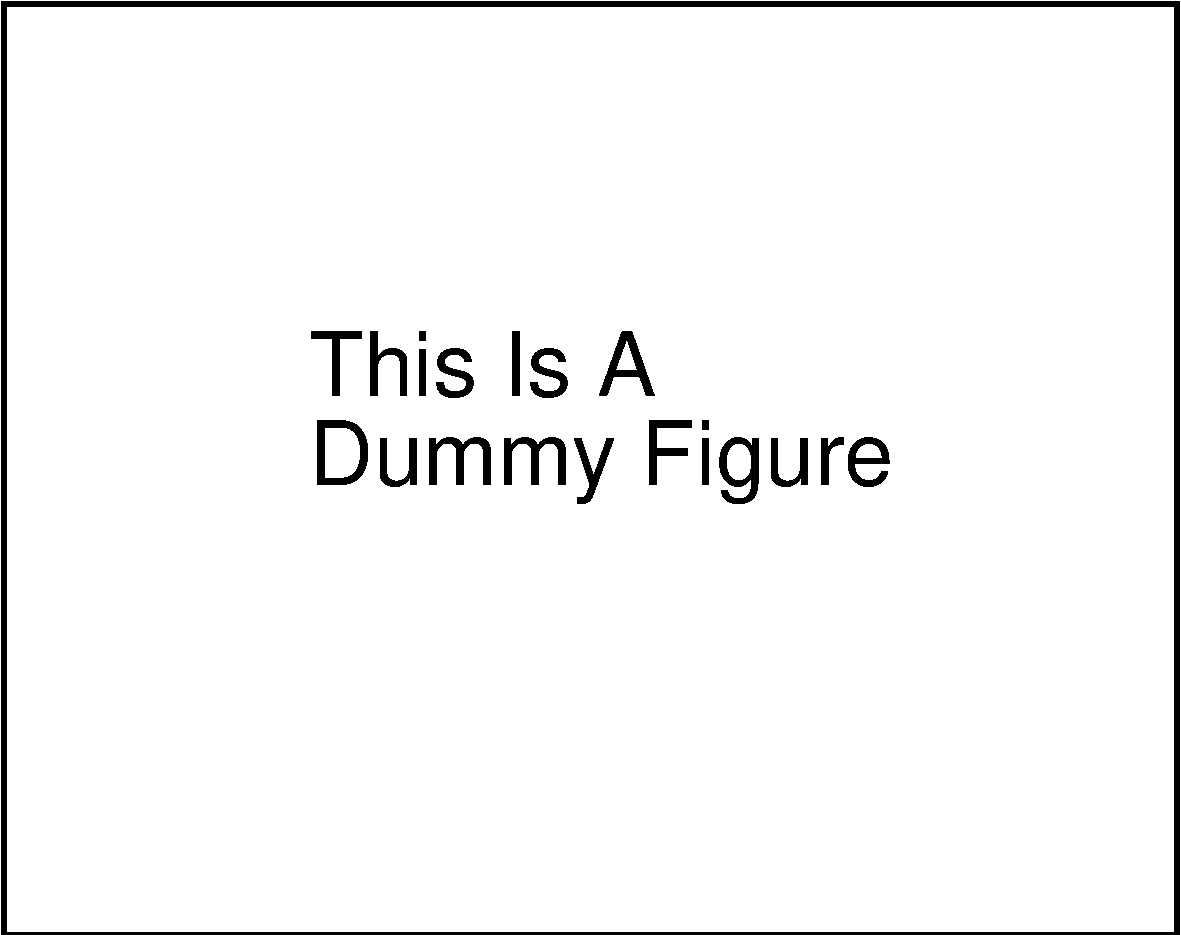
\includegraphics[width=.7\textwidth]{graphics/dummy.pdf}
%\vspace*{6.0cm}
\caption[Sensitivity of NC/CC to the strange contribution to nucleon spin]
{Sensitivity (magnitude) of the ratios ${\cal R}_{\nu p}$ (solid) and
${\cal R}_{\overline{\nu} p}$ (dashed) to a variation of the strange contribution to the
spin of the nucleon, $\Delta s$,
as a function of $Q^2$. Values greater than one imply that the relative uncertainty on $\Delta s$ is smaller than that of the corresponding ratio (see text).}
\label{fig-delta-s}
\end{figure}
The design of the %high-resolution tracker ND 
tracker includes several
different nuclear targets.  Therefore, most of the neutrino scattering
is from nucleons embedded in a nucleus, requiring nuclear effects to
be taken into account. Fortunately, in the ratio of NC/CC, the nuclear
corrections are expected to largely cancel out.  The $\Delta s$
analysis requires a good proton reconstruction efficiency as well as
high resolution on both the proton angle and energy. To this end, the
low-density %magnetized tracker at DUNE 
tracker can increase the range of the
protons inside the ND, allowing the reconstruction of proton tracks
down to $Q^2\sim0.07$~GeV$^2$. This capability will reduce the
uncertainties in the extrapolation of the form factors to the limit
$Q^2 \to 0$.
Table~\ref{tab:prange} summarizes the expected proton range for the
low-density ($\rho\sim$~\SI{0.1}{\gram\per\cubic\centi\meter}) straw-tube 
tracker (STT) in the ND tracking detector design described in
Section~\ref{sec:ndproj}.  About $2.0 (1.2) \times 10^6$ $\nu p
(\overline{\nu} p)$ events are expected after the selection cuts in
the low-density 
tracker, yielding a statistical precision on the order
of 0.1\%.
\begin{table}[htb]
\centering
\caption[Expected proton range for the  low-density tracker]{Expected proton range for the  low-density
($\rho\sim$\SI{0.1}{\gram\per\cubic\centi\meter}) tracker. The first column gives the proton kinetic energy
and the last column the proton momentum. The $Q^2$ value producing $T_p$ is calculated
assuming the struck nucleon is initially at rest.}
\label{tab:prange}
\begin{tabular}{$L^c^r^c}  %{$l^l^l^l^l^l}
\toprule
\rowtitlestyle
$ T_p$  &  $Q^2$          &  Range STT &  $P_p$  \\
\rowtitlestyle
MeV  &  GeV$^2/c^2$ &  $cm$        &  GeV$/c$ \\ 
\toprowrule
         20 &             0.038  &     4.2          & 0.195  \\ \colhline
        40 &              0.075  &   14.5          & 0.277  \\ \colhline
        60 &              0.113  &   30.3          & 0.341   \\ \colhline
        80 &              0.150  &  50.8          & 0.395  \\ \colhline
      100 &               0.188 &  75.7          & 0.445  \\ 
\bottomrule
\end{tabular}
\end{table}
The determination of $\Delta s$ in the STT %straw-tube tracker ND 
utilizes
analysis techniques performed by the FINeSSE
Collaboration~\cite{Bugel:2004yk} and used by the SciBooNE experiment.  In
particular, based on the latter, DUNE
expects a purity of about 50\%, with background contributions of 20\%
from neutrons produced outside of the detector, 10\% $\nu n$ events
and 10\% NC pion backgrounds.  The dominant systematic uncertainty
will be related to the background subtraction.  The low-energy beam
spectrum at DUNE provides the best sensitivity for this measurement
since the external background from neutron-induced proton recoils will
be reduced by the strongly suppressed high-energy tail.  The
low-density magnetized tracker is expected to increase the purity by
reducing the neutron background and the NC pion background.  The
outside neutron background, it should be noted, can be determined
using the $n \rightarrow p + \pi^-$ process in the STT.  The
sensitivity analysis is still in progress, however DUNE is confident
of achieving a precision on $\Delta s$ of about \numrange[range-phrase
= --]{0.02}{0.03}.
 
\clearpage
%%%%%%%%%%%%%%%%%%%%%%%%%%%%%%%%%%%%%%%%%%%%%%%
\section{Nucleon Structure and QCD Studies}
\label{sec-nucleon}

  Precision measurements of (anti)neutrino differential cross sections
  in the DUNE near detector will provide additional constraints on
  several key nucleon structure functions that are complementary to
  results from electron scattering experiments.
  In addition, these measurements would directly improve DUNE's
  oscillation measurements by providing accurate simulation of
  neutrino interactions in the far detector and offer an estimate of
  all background processes that are dependent upon the angular
  distribution of the outgoing particles in the far detector.
%
  Furthermore, certain QCD analyses --- i.e., global fits used for extraction of
  parton distribution functions (PDFs) via 
  the differential cross sections measured in ND data ---
  would constrain the systematic error in 
  precision electroweak measurements. This would apply  
  not only in neutrino physics but also in hadron collider measurements.  

%%%%%%%%%%%%%%%%%%%%%%%%%
\subsection{\boldmath Determination of the $F_3$
Structure Function and GLS Sum Rule}
For quantitative studies of inclusive deep-inelastic lepton-nucleon
scattering, it is vital to have precise measurements of the $F_3$
structure functions as input into global PDF fits.  Because it depends
on weak axial quark charges, the $F_3$ structure function can only be
measured with neutrino and antineutrino beams and is unique in its
ability to differentiate between the quark and antiquark content of
the nucleon.  On a proton target, for instance, the neutrino and
antineutrino $F_3$ structure functions (at leading order in
$\alpha_s$) are given by
%
\begin{eqnarray}
xF_3^{\nu p}(x) 
&=& 2 x \left( d(x) - \overline u(x) + s(x) + \cdots \right)\, , \\
%
xF_3^{\overline\nu p}(x) 
&=& 2 x \left( u(x) - \overline d(x) - \overline s(x) + \cdots \right)\, , \\ 
xF_3^{\nu n}(x) 
&=& 2 x \left( u(x) - \overline d(x) + s(x) + \cdots \right)\, , \\
%
xF_3^{\overline\nu n}(x) 
&=& 2 x \left( d(x) - \overline u(x) - \overline s(x) + \cdots \right)\, .
\end{eqnarray}
where $u_v=u-\bar u$ and $d_v=d-\bar d$ are the valence sea quark
distributions. Under the assumption of a symmetric strange sea,
i.e., $s(x)=\bar s(x)$, the above expressions show that a measurement
of the average $xF_3=(xF_3^{\nu N}+xF_3^{\bar\nu N})/2$ for neutrino
and antineutrino interactions on isoscalar targets provides a direct
determination of the valence quark distributions in the proton. This
measurement is complementary to the measurement of Drell-Yan
production at colliders, which is essentially proportional to the sea
quark distributions.
\clearpage
The first step in the structure function analysis is the measurement
of the differential cross section:
\begin{equation} 
\frac{1}{E_\nu} \frac{d \sigma^2}{dx dQ^2} = \frac{N(x,Q^2,E_\nu)}{N(E_\nu)} \frac{\sigma_{\rm tot}/E_\nu}{dx dQ^2} 
\end{equation} 
where $N(x,Q^2,E_\nu)$ is the number of events in each $(x,Q^2,E_\nu)$ bin and $N(E_\nu)$ is the number of events in each $E_\nu$ 
bin integrated over $x$ and $Q^2$. The average $xF_3$ structure function can be extracted by taking the difference between neutrino and 
antineutrino differential cross sections: 
\begin{equation} 
\frac{1}{E_\nu} \frac{d^2 \sigma^\nu}{dx dQ^2} - \frac{1}{E_\nu} \frac{d^2 \sigma^{\bar \nu}}{dx dQ^2} = 2 \left[ y \left( 1 - \frac{y}{2} \right) \frac{y}{Q^2} \right] xF_3  
\end{equation} where $xF_3$ denotes the sum for neutrino and antineutrino interactions. 
The determination of the $xF_3$ structure functions will, in turn,
allow a precision measurement of the Gross-Llewellyn-Smith (GLS) QCD
sum rule:
\begin{eqnarray}
\label{eq:GLS}
S_{\rm GLS} (Q^2) & = & 
\frac{1}{2} \int^1_0 \frac{1}{x} \left[ xF_3^{\nu N} + xF_3^{\bar \nu N} \right] dx \nonumber \\ 
& = & 3 \left[ 1 - \frac{\alpha_s(Q^2)}{\pi} - a(n_f) \left( \frac{\alpha_s(Q^2)}{\pi} \right)^2
-b(n_f) \left( \frac{\alpha_s(Q^2)}{\pi} \right)^3 \right] + \Delta {\rm HT}
\end{eqnarray}
where $\alpha_s$ is the strong coupling constant, $n_f$ is the number
of quark flavors, $a$ and $b$ are known functions of $n_f$, and the
quantity $\Delta {\rm HT}$ represents higher-twist contributions.  The
equation above can be inverted to determine $\alpha_s(Q^2)$ from the
GLS sum rule. The most precise determination of the GLS sum rule was
obtained by the CCFR experiment on an iron target~\cite{Leung:1992yx}
$S_{\rm GLS} (Q^2=3~GeV^2) = 2.50 \pm 0.018 \pm 0.078$. %The use of a
The high-resolution ND combined with the unprecedented statistics
would substantially reduce the systematic uncertainty on the low-$x$
extrapolation of the $xF_3$ structure functions entering the GLS
integral.  In addition, the presence of different nuclear targets, as
well as the availability of a target with free protons
will allow investigation of isovector and nuclear corrections, and
adding a tool to test isospin (charge) symmetry (Section~\ref{sec-isospin}).
%%%%%%%%%%%%%%%%%%%%%%%%%
\subsection{\boldmath Determination of the Longitudinal Structure Function $F_L(x,Q^2)$}
The structure
function $F_L$ is directly related to the gluon distribution
$G(x,Q^2)$ of the nucleon, as can be seen from the
Altarelli-Martinelli relation:
\begin{equation} 
F_L(x,Q^2) = \frac{\alpha_s(Q^2)}{\pi} \left[ \frac{4}{3}\int^1_x \frac{dy}{y} \left(\frac{x}{y} \right)^2 F_2(x,Q^2) + 
n_f \int^1_x \frac{dy}{y}\left(\frac{x}{y} \right)^2 \left( 1-\frac{x}{y} \right) G(y,Q^2) \right]
%2\sum_i e_i^2 \int^1_x \frac{dy}{y}\left(\frac{x}{y} \right)^2 \left( 1-\frac{x}{y} \right) G(y,Q^2) \right]  
\end{equation}  
where $n_f$ is the number of parton flavors. In the leading order 
approximation the longitudinal structure function $F_L$ is zero, while
at higher orders a nonzero $F_L(x,Q^2)$ is originated as a consequence of the violation
of the Callan-Gross relation:
\begin{equation} 
F_L(x,Q^2) = \left(  1+\frac{4M^2x^2}{Q^2} \right) F_2(x,Q^2) - 2x F_1(x,Q^2) 
\end{equation}  
where $2x F_1=F_T$ is the transverse structure function.  A
measurement of $R=F_L/F_T$ is therefore both a test of perturbative QCD at
large $x$ and a clean probe of the gluon density at small $x$ where the
quark contribution is small. A poor knowledge of $R$, especially at
small $x$, results in uncertainties in the structure functions extracted
from deep inelastic scattering cross sections, and in turn, in
electroweak measurements.  It is instructive to compare the low-$Q^2$
behavior of $R$ for charged-lepton versus  neutrino scattering. In both
cases CVC implies that $F_T \propto Q^2$ as $Q^2 \to 0$. However,
while $F_L \propto Q^4$ for the electromagnetic current, for the weak
current $F_L$ is dominated by the finite PCAC (partial conservation of
the axial current) contribution \cite{Kulagin:2007ju}.
The behavior of
$R$ at $Q^2\ll 1$ GeV$^2$ is therefore very different for
charged-lepton and neutrino scattering.  A new precision measurement
of the $Q^2$ dependence of $R$ with (anti)neutrino data would also
clarify the size of the high-twist contributions to $F_L$ and $R$,
which reflect the strength of multi-parton correlations (qq and
qg). 
The ratio of longitudinal to transverse structure functions can be
measured from the $y$ dependence of the deep inelastic scattering
data. Fits to the following function:
\begin{equation} 
F(x,Q^2, \epsilon) = \frac{\pi (1- \epsilon)}{y^2 G_F^2 M E_\nu} \left[ \frac{d^2 \sigma^\nu}{dx dy} + \frac{d^2 \sigma^{\bar \nu}}{dx dy} \right] = 2 x F_1(x,Q^2) \left[ 1 + \epsilon R(x,Q^2) \right] 
\end{equation} 
have been used by CCFR and NuTeV to determine
$R=\sigma_L/\sigma_T$. In this equation $\epsilon \simeq 2
(1-y)/(1+(1-y)^2)$ is the polarization of the virtual $W$ boson. This
equation assumes $xF_3^\nu = xF_3^{\bar \nu}$, and a correction must be
applied if this is not the case. The values of $R$ are extracted from
linear fits to $F$ versus $\epsilon$ at fixed $x$ and $Q^2$ bins.
%%%%%%%%%%%%%%%%%%%%%%%%%
\subsection{\boldmath Determination of $F_2^n$ and the $d/u$ Ratio of Quark Distribution Functions}
Because of the larger electric charge on the $u$ quark than on the
$d$, the electromagnetic proton $F_2$ structure function data provide
strong constraints on the $u$-quark distribution, but are relatively
insensitive to the $d$-quark distribution.  To constrain the $d$-quark
distribution a precise knowledge of the corresponding $F_2^n$
structure functions of free neutrons is required, which in current practice is
%currently 
extracted from inclusive deuterium $F_2$ data.  At large values of $x$
($x>0.5$) the nuclear corrections in deuterium become large and, more
importantly, strongly model-dependent, leading to large uncertainties
on the resulting $d$-quark distribution.  Using the isospin relation
$F_2^{\bar \nu p} = F_2^{\nu n}$ and $F_2^{\nu p} = F_2^{\bar \nu n}$
it is possible to obtain a direct determination of $F_2^{\nu n}$ and
$F_2^{\bar \nu n}$ with neutrino and antineutrino scattering off a target with free
protons. This determination is free from model uncertainties
related to nuclear targets. The extraction of $F_2^{\nu n}$ and
$F_2^{\bar \nu n}$ will allow a precise extraction on the $d$-quark
distribution at large $x$.  Existing neutrino data on hydrogen  
have relatively large errors and do not extend beyond
$x\sim0.5$~\cite{Bodek:1985tv,Jones:1987gk}.
The $F_2^{\bar \nu p}$ and $F_2^{\nu p}$ structure functions can be
obtained from interactions on a target with free protons  after subtracting
the contributions from $xF_3$ and $R$. These latter can either be
modeled within global PDF fits or taken from the other two
measurements described above. As discussed in Section~\ref{sec-isospin} the DUNE 
ND can achieve competitive measurements of $F_2^{\bar \nu p}$ and $F_2^{\nu p}$ 
with an increase of statistics of three orders of magnitude with respect to the 
existing hydrogen data~\cite{Bodek:1985tv,Jones:1987gk}. 
%%%%%%%%%%%%%%%%%%%%%%%%%
\subsection{Measurement of Nucleon Structure Functions}
At present neutrino scattering measurements of cross sections have
considerably larger uncertainties than those of the electromagnetic
inclusive cross sections.  The measurement of the differential cross
sections~\cite{Formaggio:2013kya} is dominated by three
uncertainties: (1) muon energy scale, (2) hadron energy scale, and (3)
knowledge of the input (anti)neutrino flux.  Table~\ref{tab:expcomp}
shows a comparison of past and present experiments and the
corresponding uncertainties on the energy scales.  The most precise
measurements are from the CCFR, NuTeV and NOMAD experiments, which are
limited to a statistics of about \num{e6} neutrino events.
%
\begin{dunetable}[Structure function measurements from previous experiments]{lccccrr}{expcomp}
  {Summary of past experiments performing structure function measurements. The expected numbers in the DUNE near detector for a five-year run with the \SIadj{1.2}{\MW} \SIadj{120}{\GeV} reference beam  ($5 \times 10^{21}$ POT) are also given for comparison.}  
Experiment & Mass & \multicolumn{1}{c}{\numu CC Stat.} & Target & $E_\nu$ (GeV)
& $\Delta E_\mu$  & $\Delta E_{\rm H}$ \\ \toprowrule
            CDHS~\cite{Berge:1989hr} &  750 t &  { $10^{7}$}   &  p,Fe & 20-200 & 2.0\% & 2.5\% \\ \colhline
%    CHARM II  &  547 t  & { $10^{7}$}  & SiO$_2$ & 20-200 & & \\
            BEBC~\cite{Allasia:1983vw,Allasia:1985hw} & various &   5.7$\times$$10^{4}$   & p,D,Ne & 10-200 &  & \\ \colhline
            CCFR~\cite{Yang:2000ju,Yang:2001xc} & 690 t & { 1.0$\times$$10^{6}$}   & Fe & 30-360 & 1.0\% & 1.0\% \\  \colhline
            NuTeV~\cite{Tzanov:2005kr} &  690 t & { 1.3$\times$$10^{6}$}  &  Fe &  30-360 &  0.7\% &  0.43\% \\ \colhline
            CHORUS~\cite{Onengut:2005kv} & 100 t & { 3.6$\times$$10^{6}$}   &  Pb &  10-200 &  2.5\% &  5.0\% \\ \colhline
            NOMAD~\cite{Wu:2007ab} & 2.7 t & { 1.3$\times$$10^{6}$}   &  C &  5-200 &  0.2\% &  0.5\% \\ \colhline
            ~~~~~~~~~~~~~~~~~\cite{Samoylov:2013xoa}     & 18 t & { 1.2$\times$$10^{7}$}   &  Fe  &  5-200 &  0.2\% &  0.6\% \\ \colhline
            MINOS ND~\cite{Adamson:2009ju} & 980 t &  3.6$\times$$10^{6}$   &  Fe & 3-50 & 2-4\% & 5.6\% \\  \colhline
            DUNE ND  & 5 t &  5.9$\times$$10^{7}$   & (C$_3$H$_6$)$_n$  & 0.5-30 & $<0.2$\% & $<0.5$\% \\  \bottomrule
\end{dunetable} 

The MINER$\nu$A~\cite{Osmanov:2011ig} experiment is expected to provide new structure
function measurements on a number of nuclear targets including He, C,
Fe and Pb in the near future.  Since the structure function
measurement mainly involves DIS events, the MINER$\nu$A measurement
will achieve a competitive statistics after the completion of the new
run with the medium-energy beam. 
MINER$\nu$A will focus on a measurement of the ratio of different nuclear
targets to measure nuclear corrections in (anti)neutrino
interactions. It must be noted that the MINER$\nu$A experiment relies
on the MINOS ND for muon identification.  The corresponding
uncertainty on the muon-energy scale (Table~\ref{tab:expcomp}) is
substantially larger than that in other modern experiments, e.g.,
NuTeV and NOMAD, thus limiting %. This fact would limit 
the potential of absolute
structure function measurements. Furthermore, the muon-energy scale is
also the dominant source of uncertainty in the determination of the
(anti)neutrino fluxes with the low-$\nu$ method.  Therefore, the flux
uncertainties in MINER$\nu$A are %also 
expected to be larger than in
NOMAD and NuTeV. 
 
Given its reference beam design and \MWadj{1.2} proton-beam power, DUNE
expects to collect about \num{2.3e7} neutrino DIS events and
about \num{4.4e6}  antineutrino DIS events in the ND. 
These numbers correspond to an improvement
by more than one order of magnitude with respect to the most precise
past experiments, e.g., NuTeV~\cite{Tzanov:2005kr} and 
NOMAD~\cite{Wu:2007ab,Samoylov:2013xoa}. 
With these high-statistics
samples, DUNE will be able to significantly reduce the gap between the
uncertainties on the weak and electromagnetic structure functions.
A possible high-energy run with the upgraded \MWadj{2.3} beam would offer a 
further increase by more than a factor of ten in statistics.  
In addition to the large data samples, the use of a high-resolution,
low-density spectrometer allows DUNE to reduce systematic
uncertainties with respect to previous measurements. The DUNE ND is
expected to achieve precisions better than 0.2\% and 0.5\% on the muon-
and hadron-energy scales, respectively. 
These numbers are based on the results achieved by the NOMAD experiment
(Table~\ref{tab:expcomp}), which had %a much smaller statistics 
much lower statistics and
poorer resolution than is expected in the DUNE ND. The calibration of the momentum and energy scales
will be performed with the large sample of reconstructed $K^0_S \to \pi \pi$,
$\Lambda \to p \pi$, and $\pi^0 \to \gamma \gamma$ decays.
In addition, the overall hadronic energy scale can be calibrated by exploiting the
well-known structure of the Bjorken $y$ distribution in (anti)neutrino DIS
interactions~\cite{Wu:2007ab,Petti:2011zz}.
%  
The relative fluxes as a function of energy can be extracted to a precision of 
about 2\% with the low-$\nu$ method, due to the small uncertainty on the muon-energy
scale. The world average absolute normalization of the differential
cross sections $\sigma_{\rm tot}/E$, is known to 2.1\%
precision~\cite{Beringer:1900zz}. 
However, with the \MWadj{1.2} beam available from the PIP-II
upgrades, it will be possible to improve the absolute normalization
using $\nu$-e NC elastic scattering events, coherent meson production, etc. 
An overall precision of 1-2\% would make (anti)neutrino
measurements comparable to or better than the complementary measurements from
charged-lepton DIS.
On the time scale of %the DUNE project
DUNE, comparable measurements from
(anti)neutrino experiments are not expected, primarily due to the low
energy of competing beamlines (J-PARC neutrino beamline in Japan~\cite{Sekiguchi:2012xma}) or to the poorer resolution of the detectors
used (MINER$\nu$A~\cite{Osmanov:2011ig} , T2K~\cite{Abe:2011ks},
NO$\nu$A~\cite{Ayres:2007tu}). The %main 
experimental program %that can
most likely to compete with the DUNE ND measurements is the \GeVadj{12} upgrade at
Jefferson Laboratory (JLab)~\cite{Dudek:2012vr}.  However, it must be
emphasized that the use of electron beams at JLab makes this program
\emph{complementary} to DUNE's.  In particular, the three topics
discussed above are specific to the (anti)neutrino interactions.
Several planned experiments at JLab with the energy-upgraded \GeVadj{12}
beam will measure the $d/u$ ratio from D targets up to $x\sim0.85$, 
using different methods to minimize the nuclear corrections.  
The DUNE measurement %in the ND 
will be competitive with the
proposed JLab \GeVadj{12} experiments, since the large statistics expected will allow
a precise determination of $F_2^{\nu
  n}$ and $F_2^{\bar \nu n}$ up to $x\sim0.85$. Furthermore,
the use of a weak probe coupled with a wide-band beam will provide
a broader $Q^2$ range than in JLab experiments, thus allowing a separation of
higher twist and other sub-leading effects in $1/Q^2$.
%%%%%%%%%%%%%%%%%%%%%%%%%%%%%%%%%%%%%%%%%%%%%%%
\section{Tests of Isospin Physics and Sum-Rules}
%\section{Isospin Physics and Sum-Rules}
\label{sec-isospin}

One of the most compelling physics topics accessible to DUNE's high-resolution near detector is the isospin physics using neutrino and antineutrino interactions. This physics involves the Adler sum rule and tests isospin (charge) symmetry in nucleons and nuclei.

The Adler sum rule relates the integrated difference of the
antineutrino and neutrino $F_2$ structure functions to the isospin of the target:
%
\begin{equation}
\label{ASR}
{\cal S}_A (Q^2) =\int_0^1 \; dx \; \left[ F_2^{\overline\nu} (x,Q^2) - F_2^{\nu}(x,Q^2) \right]/(2x)
= 2\,I_z,
\end{equation}
%
where the integration is performed over the entire kinematic range of the
Bjorken variable $x$ and $I_z$ is the projection of
the target isospin vector on the quantization axis ($z$ axis).
For the proton ${\cal S}_A^{p}=1$ and for the neutron ${\cal S}_A^{n}=-1$.
In the quark-parton model the Adler sum is the difference between the
number of valence $u$ and $d$ quarks of the target. The Adler sum rule
survives the strong-interaction effects because of the conserved vector 
current (CVC) and provides an
exact relation to test the local current commutator algebra of the weak
hadronic current. %We note that 
In the derivation of the Adler sum rule the effects of both
non-conservation of the axial current and heavy-quark production are
neglected. 
Experimental tests of the Adler sum rule require the use of a hydrogen target
to avoid nuclear corrections to the bound nucleons inside the nuclei.
The structure functions $F_2^{\overline{\nu}}$ and $F_2^\nu$ have to be determined
from the corresponding differential cross sections and must be extrapolated
to small $x$ values in order to evaluate the integral. %~(\ref{ASR}). 
The test performed in bubble chambers by the BEBC
Collaboration --- the only test available ---  is limited by the modest statistics;
it used about 9,000 $\overline{\nu}$ and 5,000 $\nu$ events
collected on hydrogen~\cite{Allasia:1985hw}.
The DUNE program can provide the first high-precision test of the
Adler sum rule.  To this end, the use of the high-energy beam tune
shown in Figure~\ref{fig:beamtunes}, although not essential, would
increase the sensitivity, allowing attainment of higher $Q^2$
values. Since the use of a liquid H$_2$ bubble chamber is excluded in
the ND hall due to safety concerns, the (anti)neutrino interactions
off a hydrogen target can only be extracted with a subtraction method
from the composite materials of the ND targets.  Using this technique
to determine the position resolution in the location of the primary
vertex is crucial to reducing systematic uncertainties.  For this
reason, a precision test of the Adler sum rule is best performed with
the low-density magnetized ND.
A combination of two different targets --- the polypropylene
$(C_3H_6)_n$ foils placed in front of the STT modules and pure carbon
foils --- are used in the low-density, magnetized 
ND to provide a
fiducial hydrogen mass of about 1 t.  With the DUNE fluxes from
the standard exposure, $5.0(1.5) \times 10^6 \pm 13(6.6)\times 10^3
(sub.)$ $\nu(\overline{\nu})$ CC events (where the quoted uncertainty is dominated by the
statistical subtraction procedure) %about \num{1e6} inclusive
%$\nu(\overline{\nu})$ CC events 
would be collected on the hydrogen
target.  The level of precision that can be achieved is sufficient to
open up the possibility of making new discoveries in the quark and
hadron structure of the proton. No other comparable measurement is
expected on the timescale of DUNE.
%%%%%%%%%%%%%%%%%%%%%%%%%%%%%%%%%%%%%%%%%%%%%%%
\section{Studies of (Anti)Neutrino-Nucleus Interactions} 
\label{sec-nuclear} 
An integral part of the physics program envisioned for the DUNE ND
involves detailed measurements of (anti)neutrino interactions in a
variety of nuclear targets.  The DUNE ND offers substantially
larger statistics coupled with a much higher resolution and, in turn,
lower systematic uncertainties with respect to past experiments
(Table~\ref{tab:expcomp}) or ongoing and future ones
(MINER$\nu$A~\cite{Osmanov:2011ig}, T2K~\cite{Abe:2011ks},
NO$\nu$A~\cite{Ayres:2007tu}).  The most important nuclear target is
of course the argon target, which matches the DUNE far detector.
%Regarding 
The ND standard target is polypropylene
(C$_3$H$_6$)$_n$, largely provided by the mass of the STT radiators.
%
An additional proposed ND target is argon gas in pressurized aluminum
tubes with sufficient mass to provide $\simeq$10 times the \numu CC and
NC statistics as expected in the DUNE far detector.  Equally important
nuclear targets are carbon (graphite), which is essential in order to
get (anti)neutrino interactions on free protons through a statistical
subtraction procedure from the main polypropylene target 
(Section~\ref{sec-isospin}), and calcium.  In particular, this latter
target has the same atomic weight ($A=40$) as argon but is
isoscalar. One additional nuclear target is iron, which is used in the
proposed India-based Neutrino Observatory
(INO)~\cite{Mondal:2012fn}. %Indeed t
The modularity of the STT provides for successive measurements using
thin nuclear targets (thickness $< 0.1 X_0$), while the excellent
angular and space resolution allows a clean separation of events
originating in different target materials.  Placing an arrangement of
different nuclear targets upstream of the detector
provides the desired nuclear samples in (anti)neutrino interactions.
For example, a single \SIadj{7}{\milli\meter}-thick calcium layer at the upstream 
end of the detector will provide  
about \num{3.1e5} \numu CC interactions in one year. 
%
Potential ND studies in nuclear effects include the following: 
%
\begin{itemize}%[parsep=-2pt]
\item nuclear modifications of form factors
\item nuclear modifications of structure functions
\item mechanisms for nuclear effects in coherent and incoherent regimes
\item a dependence of exclusive and semi-exclusive processes
\item effect of final-state interactions
\item effect of short-range correlations
\item two-body currents
\end{itemize}
The study of nuclear effects in (anti)neutrino interactions off nuclei
is directly relevant for the long-baseline oscillation studies.  The
use of heavy nuclei like argon in the DUNE far detector requires a measurement
of nuclear cross sections on the same targets in the ND in order to reduce signal 
and background uncertainties in the oscillation analyses.  Cross-section
measurements obtained from other experiments using different nuclei
are not optimal; in addition to the different $p/n$ ratio in argon
compared to iron or carbon where measurements from other experiments
exist, nuclear modifications of cross sections can differ from 5\% to
15\% between carbon and argon for example, while the difference in the
final-state interactions could be larger.
%~\cite{docdb740}.
Additionally, nuclear modifications can introduce a substantial
smearing of the kinematic variables reconstructed from the observed
final-state particles.  Detailed measurements of the dependence on the
atomic number $A$ of different exclusive processes are then required
in order to understand the absolute energy scale of neutrino event
interactions and to reduce the corresponding systematic uncertainties
on the oscillation parameters.
It is worth noting that the availability of a free-proton target
through statistical subtraction of the (C$_3$H$_6$)$_n$ and carbon
targets (Section~\ref{sec-isospin}) will allow for the first time a
direct model-independent measurement of nuclear effects --- including
both the primary and final-state interactions --- on the argon target
relevant for the far detector oscillation analysis.
Furthermore, an important question in nuclear physics is how the
structure of a nucleon is modified when said nucleon is inside the
medium of a heavy nucleus as compared to a free nucleon like the
proton in a hydrogen nucleus.  Studies of the ratio of structure
functions of nuclei to those of free nucleons (or in practice, the
deuteron) reveal nontrivial deviations from unity as a function of $x$
and $Q^2$.  These have been well explored in charged-lepton scattering
experiments, but little empirical information exists from neutrino
scattering. Measurements of structure using neutrino scattering are
complementary to those in charged-lepton scattering.
Another reason to investigate the nuclear-medium modifications 
of neutrino structure functions is that most neutrino scattering
experiments are performed on nuclear targets, from which information
on the free nucleon is inferred by performing a correction for the
nuclear effects.  
%
In practice this often means applying the same nuclear correction as
for the electromagnetic structure functions, which introduces an
inherent model-dependence in the result.  In particular, significant
differences between photon-induced and weak-boson-induced nuclear
structure functions are predicted, especially at low $Q^2$ and low
$x$, which have not been tested.  A striking example is offered by the
ratio $R$ of the longitudinal-to-transverse structure
functions~\cite{Kulagin:2007ju}.  While the electromagnetic ratio tends
to zero in the photoproduction limit, $Q^2 \to 0$, by current
conservation, the ratio for neutrino structure functions is predicted
to be \emph{finite} in this limit.  Thus, significant discovery
potential exists in the study of neutrino scattering from nuclei.
The comparison of argon and calcium targets (${}^{40}_{18}$Ar and
${}^{40}_{20}$Ca) in the DUNE ND would be particularly
interesting. Since most nuclear effects depend on the atomic weight
$A$, inclusive properties of (anti)neutrino interactions are expected
to be the same for these two
targets~\cite{Kulagin:2007ju,Butkevich:2012zr,Butkevich:2007gm,Ankowski:2007uy}.
This fact would allow the use of both targets to model signal and
backgrounds in the DUNE far detector (argon target), as well as to
compare DUNE results for nuclear effects on argon with the extensive
data on calcium from charged lepton DIS. In addition, a high-precision
measurement of (anti)neutrino interactions in both argon and calcium
opens the possibility for studying a potential flavor and isovector
dependence of nuclear effects and to further test the isospin (charge
symmetry) in nuclei (Section~\ref{sec-isospin}).  Evidence for any
of these effects would constitute important discoveries.
Finally, the extraction of (anti)neutrino interactions on deuterium
from the statistical subtraction of H$_2$O from D$_2$O, which is
required to measure the fluxes (Section~\ref{sec-fluxosc}), would
allow the first direct measurement of nuclear effects in deuterium.
This measurement can be achieved since the structure function of a
free isoscalar nucleon is given by the average of neutrino and
antineutrino structure functions on hydrogen ($F_2^{\nu
  n}=F_2^{\overline{\nu} p}$).  A precise determination of nuclear
modifications of structure functions in deuterium would play a crucial
role in reducing systematic uncertainties from the global PDF fits.
%%%%%%%%%%%%%%%%%%%%%%%%%%%%%%%%%%%%%%%%%%%%%%%
\section{Search for Heavy Neutrinos} 

  The most economical way to handle the problems of neutrino masses,
  dark matter and the Baryon Asymmetry of the Universe in a unified
  way may be to add to the Standard Model (SM) three Majorana singlet
  fermions with masses roughly on the order of the masses of known
  quarks and leptons using the seesaw
  mechanism~\cite{Yanagida:1980xy}. The appealing feature of this
  theory (called the $\nu$MSM for \emph{Neutrino Minimal
    SM})~\cite{Asaka:2005pn} is that every left-handed fermion has a
  right-handed counterpart, leading to a consistent way of treating
  quarks and leptons.
  The most efficient mechanism proposed for producing these heavy
  sterile singlet states experimentally is through weak decays of
  heavy mesons and baryons, as can be seen from the left-hand diagram
  in Figure~\ref{fig:production-and-decays}, showing some examples of
  relevant two- and three-body decays~\cite{Gorbunov:2007ak}. These
  heavy mesons can be produced by energetic protons scattering off the
  DUNE neutrino production target and the heavy singlet neutrinos from their
  decays detected in the near detector.

\begin{figure}[!htb]
\centering
\tikzset{
  quark/.style={draw=blue, postaction={decorate},
    decoration={markings,mark=at position .6 with {\arrow[draw=blue]{>}}}},
  electron/.style={draw=pink, postaction={decorate},
    decoration={markings,mark=at position .6 with {\arrow[draw=blue]{>}}}},
  neutrino/.style={draw=red, postaction={decorate},
    decoration={markings,mark=at position .6 with {\arrow[draw=blue]{>}}}},
  heavy/.style={draw=red, postaction={decorate},
    decoration={markings,mark=at position .6 with {\arrow[draw=blue]{>}}}},
  pion/.style={draw=black,postaction={decorate},
    decoration={markings,mark=at position .6 with {\arrow[draw=blue]{>}}}},
  muon/.style={draw=purple, postaction={decorate},
    decoration={markings,mark=at position .6 with {\arrow[draw=blue]{>}}}},
  gamma/.style={decorate, decoration={snake,amplitude=4pt, segment length=5pt}, draw=red},
}
  \begin{minipage}[h]{0.45\textwidth}
    \begin{center}
  \begin{tikzpicture}[ultra thick,scale=0.25]
    \draw[quark] (-10,0) -- node[black,above,sloped] {$D_S$} (0,0);
    \draw[muon] (0,0) -- node[black,above,sloped] {$\mu$} (10,2);
    \draw[neutrino] (0,0) -- node[black,below,sloped] {$\nu_\mu$} (5,-1) node{$\circ$};
    \draw[heavy] (5,-1) -- node[black,below,sloped] {$N_{2,3}$} (10,-2);
  \end{tikzpicture}
  \begin{tikzpicture}[ultra thick,scale=0.25]
    \draw[quark] (-10,0) -- node[black,above,sloped] {$D$} (0,0);
    \draw[muon] (0,0) -- node[black,above,sloped] {$\mu$} (10,2);
    \draw[pion] (0,0) --  (10,0) node[black,below,sloped] {$\pi$};
    \draw[neutrino] (0,0) -- node[black,below,sloped] {$\nu_\mu$} (5,-1) node{$\circ$};
    \draw[heavy] (5,-1) -- node[black,below,sloped] {$N_{2,3}$} (10,-2);
  \end{tikzpicture}
    \end{center}
  \end{minipage}%
  \begin{minipage}[h]{0.45\textwidth}
    \begin{center}
  \begin{tikzpicture}[ultra thick,scale=0.25]
    \draw[heavy] (-10,0) -- node[black,above,sloped] {$N_{2,3}$} (-5,0) node{$\circ$};
    \draw[neutrino] (-5,0) -- node[black,above,sloped] {$\nu_\mu$} (0,0);
    \draw[muon] (0,0) -- node[black,above,sloped] {$\mu$} (10,2);
    \draw[pion] (0,0) -- node[black,below,sloped] {$\pi$} (10,-2);
  \end{tikzpicture}
  \begin{tikzpicture}[ultra thick,scale=0.25]
    \draw[heavy] (-10,0) -- node[black,above,sloped] {$N_{2,3}$} (-5,0) node{$\circ$};
    \draw[neutrino] (-5,0) -- node[black,above,sloped] {$\nu_\mu$} (0,0);
    \draw[muon] (0,0) -- node[black,above,sloped] {$\mu$} (10,2);
    \draw[electron] (0,0) -- (10,0) node[black,below,sloped] {$e$};
    \draw[neutrino] (0,0) -- node[black,below,sloped] {$\nu_e$} (10,-2);
  \end{tikzpicture}
    \end{center}
  \end{minipage}
\caption[Feynman diagrams pertaining to sterile neutrinos]{Left: Feynman  diagrams of meson decays producing
heavy sterile neutrinos. Right: Feynman diagrams of sterile-neutrino decays.}
\label{fig:production-and-decays}
\end{figure}
The lightest of the three new singlet fermions in the $\nu$MSM, is
expected to have a mass from \SIrange{1}{50}{\keV}~\cite{Boyarsky:2009ix} 
and could play the role of the dark matter particle~\cite{Dodelson:1993je}. 
The two other neutral fermions are
responsible for giving mass to ordinary neutrinos via the seesaw
mechanism at the {\em electroweak scale} and for creation of the
Baryon Asymmetry of the Universe (BAU; for a review
see~\cite{Boyarsky:2009ix}). The masses of these particles and their
coupling to ordinary leptons are constrained by particle physics
experiments and cosmology~\cite{Gorbunov:2007ak,Atre:2009rg}. 
They should be almost degenerate, thus nearly forming Dirac fermions (this is
dictated by the requirement of successful baryogenesis). Different
considerations indicate that their mass should be in the region of
${\cal O}(1)$~GeV~\cite{Shaposhnikov:2008pf}.  The mixing angle,
$U^2$, between the singlet fermions and the three active-neutrino
states must be small~\cite{Asaka:2005pn,Akhmedov:1998qx} 
--- otherwise the large mixing
would have led to equilibration of these particles in the early
Universe above the electroweak temperatures, and, therefore, to
erasing of the BAU --- explaining why these new particles
have not been seen previously.
Several experiments have conducted searches for heavy neutrinos, for
example BEBC~\cite{CooperSarkar:1985nh}, \linebreak
CHARM~\cite{Bergsma:1985is},
NuTeV~\cite{Vaitaitis:1999wq} and the CERN PS191
experiment~\cite{Bernardi:1985ny,Bernardi:1987ek} (see also a discussion
of different experiments in~\cite{Atre:2009rg}). 
In the search for heavy
neutrinos, the strength of the DUNE %high-resolution 
ND, compared
to earlier experiments, lies in reconstructing the exclusive decay
modes, including electronic, hadronic and muonic.  Furthermore, the
detector offers a means to constrain and measure the backgrounds using
control samples. 
In case of the DUNE experiment the relevant heavy mesons are charmed. %ones. 
With a typical lifetime (in the rest frame) of about
\SI{e-10}{s}, %$10^{-10}$~s 
these mesons mostly decay before further interaction,
yielding the sterile-neutrino flux.  Since these sterile neutrinos are
very weakly interacting they can cover quite a large distance before
decay, significantly exceeding the distance of roughly \SI{500}{\meter} from the target
to the ND.  The ND can search for decays of neutrinos into SM particles due
to mixing with active neutrinos,
provided a sufficiently long instrumented decay region is available.
Two examples of the interesting decay modes are presented on the right
panel of Figure~\ref{fig:production-and-decays}. More examples can be found
in~\cite{Gorbunov:2007ak}. 
An estimate of sterile-neutrino events that can be observed in the
DUNE ND, $N^{DUNE}_{signal}$, is obtained by comparing the
relevant parameters of the DUNE and CHARM experiments.  The number of
events grows linearly with the number of protons on target, the number
of produced charmed mesons, the detector length (decay region) and the
detector area.  In particular, this latter linear increase   is valid if the
angular spread of the neutrino flux, which is on the order of
$N_mM_D/E_{beam}$, is larger than the angle at which the ND is seen
from the target.  Here $N_m$ is the multiplicity of the produced
hadrons, and the above condition is valid for both DUNE and CHARM. The
number of events %also 
decreases linearly when the energy increases,
since this increases the lifetime, reducing the decay probability within
the detector.  Finally, the number of mesons decreases quadratically
with the distance between the target and the detector.
The considerations above imply that a search for $\nu$MSM sterile
neutrinos in the DUNE ND can be %already
competitive after only five years of running with the reference beam,
corresponding to an overall integrated exposure of about \num{5e21}
POT with a proton energy of \SI{120}{GeV}.  The use of a low-density,
high-resolution spectrometer in the ND substantially reduces
backgrounds and allows the detection of both leptonic and hadronic
decay modes.  Assuming a fiducial length of the magnetized tracker of
\SI{7}{m} as decay region, the ratio between the signal event to be
observed in the DUNE ND and those in the CHARM experiment can be
estimated to be more than a factor of 50 after only four years of
running.  Since both production and decay rates are proportional to
the square of the neutrino mixing angles, the corresponding
improvement in the square of the neutrino mixing angle $U^2$ will be
about a factor of seven with respect to the CHARM
experiment. Figure~\ref{fig:heavynu} shows the projected DUNE
sensitivity in the $(U^2,M)$ plane.  At lower values of the mass of
the heavy neutrinos, additional constraints can be obtained for kaons
by comparing the DUNE and PS191 experiments, as shown in
Figure~\ref{fig:heavynu}.
%
\begin{figure}[!htb]
\centerline{
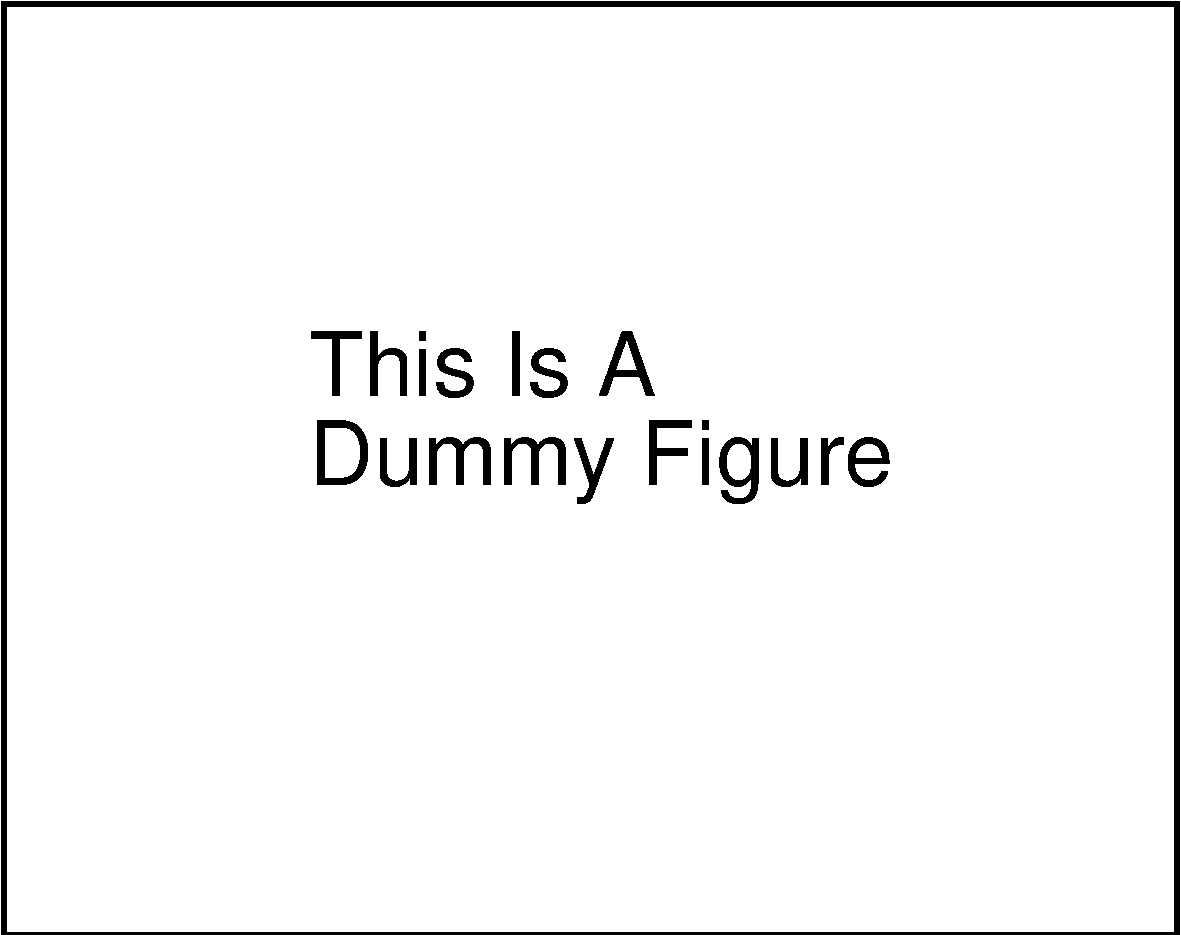
\includegraphics[width=0.5\textwidth]{graphics/dummy.pdf}
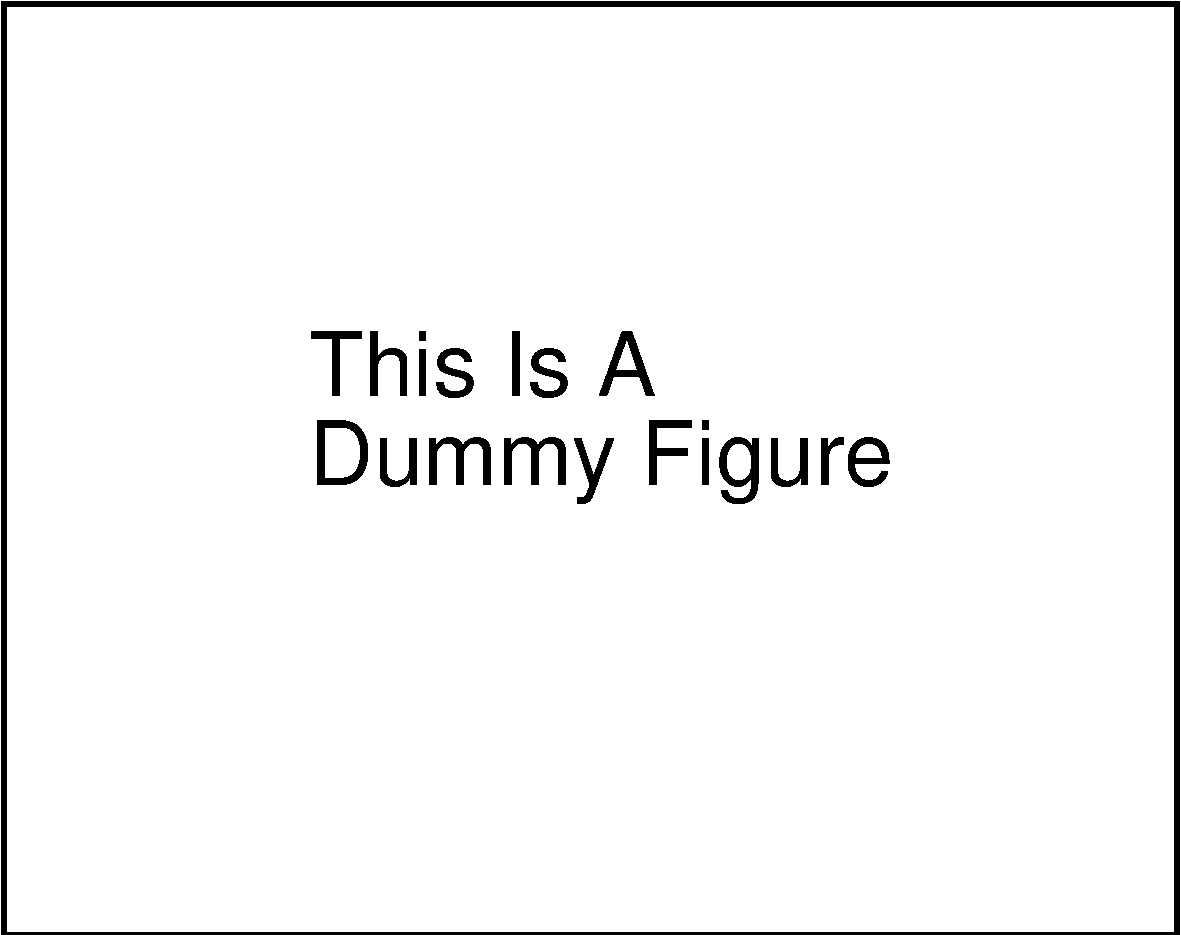
\includegraphics[width=0.5\textwidth]{graphics/dummy.pdf}}
\caption[Near detector constraints on heavy Majorana neutrinos]
{Upper limits on $U^2$, the mixing angle between heavy sterile
  neutrinos and the light active states, coming from the Baryon
  Asymmetry of the Universe (solid lines), from the seesaw mechanism
  (dotted line) and from the Big Bang nucleosynthesis (dotted
  line). The regions corresponding to different experimental searches
  are outlined by blue dashed lines. Left panel: normal hierarchy;
  right panel: inverted hierarchy (adopted
  from~\cite{Canetti:2010aw}).  Pink and red curves indicate the
  expected sensitivity of the DUNE near detector with an exposure of
  $5\times 10^{21}$ POT ($\sim 5$ years) with the \MWadj{1.2}
  reference beam at 120 GeV for detector lengths of \SI{7}{m} and
  \SI{30}{m} , respectively (see text for details).}
\label{fig:heavynu}
\end{figure}
%
It must be noted that exploitation of the complete 5 + 5 years ($\nu$ + $\overline\nu$) years 
of data taking would further improve the number of expected
events by a factor of  two, since it %this latter
scales linearly with the number of protons on target.  With the beam
upgrade to \SIadj{2.3}{MW}, this improvement would become a factor of
four with respect to the initial five year run and the %standard
\SI{1.2}{MW} beam.
A better sensitivity to $\nu$MSM can be achieved by instrumenting the
upstream region of the ND hall (e.g., with the liquid argon detector and some
minimal tracking device upstream). The fiducial volume of the new
detector will need to be empty (material-free) or fully sensitive in order
to suppress background events. The geometry of the ND hall would allow
a maximal decay length of about \SI{30}{m}. The sensitivity of this
configuration can be estimated by rescaling the expected limits on
the neutrino mixing angle $U^2$. The expected number of signal events with a total decay
length of $\sim30$~m exceeds by about 200 (800) times the number of
events in CHARM after a five (5 +5) year run with the standard (upgraded)
beam. In turn, this implies an improvement by a factor of 15 (28) in
the sensitivity to $U^2$ with respect to the CHARM experiment.
%It must be noted that i -------------   repetitive from 2 pgraphs up
If the magnetic moment of the sterile neutrinos
is sizeable, the dominant decay channel would be a radiative
electromagnetic decay into $\gamma \nu$, which has also been proposed
as a possible explanation for the observed MiniBooNE low-energy
excess~\cite{AguilarArevalo:2008rc}. This possibility,  in turn, requires a detector
capable of identifying and reconstructing single photon events.  The
low-density ND in DUNE can achieve an excellent 
sensitivity to this type of search as demonstrated by a similar analysis in
NOMAD~\cite{Kullenberg:2011rd}.
%%%%%%%%%%%%%%%%%%%%%%%%%%%%%%%%%%%%%%%%%%%%%%%
%\section{Search for High $\boldsymbol{\Delta m^2}$ Neutrino Oscillations}
\section{Search for High $\Delta m^2$ Neutrino Oscillations}
\fixme{removed bold. anne}
%\section{Search for Non-Standard Interactions: High $\Delta m^2$ Neutrino Oscillations}
\label{sec-high-delmsq}
The evidence for neutrino oscillations obtained from atmospheric,
long-baseline accelerator, solar and long-baseline reactor data from
different experiments consistently indicates two different scales,
with $\Delta m_{32}^2\sim$\SI{2.4e-3}{\eV^2} defining the
atmospheric oscillations (also long-baseline accelerator and
short-baseline reactor scales) and $\Delta m_{21}^2\sim$\SI{7.9e-5}{\eV^2} defining the solar oscillations (and long-baseline
reactor oscillations).  The only way to accommodate oscillations with
relatively high $\Delta m^2$ at the \si{\eV^2} scale as suggested by the
results from the LSND experiment~\cite{Volpe:2001qe} is therefore to
add one or more sterile 
neutrinos to the conventional three light
neutrinos.
Recently, the MiniBooNE experiment reported that its antineutrino
data might be consistent with the LSND $\overline{\nu}_\mu \to \overline{\nu}_e$
oscillation with $\Delta m^2\sim$ \si{\eV^2}~\cite{Maltoni:2007zf}.
Contrary to the antineutrino data, the %MiniBooNE 
neutrino data seem to
exclude high $\Delta m^2$ oscillations, possibly indicating a 
different behavior between neutrinos and antineutrinos.
Models with five (3+2) or six (3+3) neutrinos can potentially explain
the MiniBooNE results. In addition to the cluster of the three neutrino
mass states (accounting for \emph{solar} and \emph{atmospheric} mass splitting), two
(or three) states at the eV scale are added, with a small
admixture of $\nu_e$ and $\nu_\mu$ to account for the LSND signal. 
One distinct prediction from such models is a significant probability
for $\overline{\nu}_\mu$ disappearance into sterile neutrinos, on the order
of 10\%, in addition to the small probability for $\overline{\nu}_e$ appearance.

  Given a roughly \SIadj{500}{m} baseline and a low-energy beam, the DUNE ND
  can reach the same value $L/E_\nu$ as MiniBooNE and LSND. The
  large fluxes and the availability of fine-grained detectors make the
  DUNE program well suited to search for active-sterile neutrino
  oscillations beyond the three-flavor model with $\Delta m^2$ at the
  eV$^2$
  scale. 

Due to the potential differences between neutrinos and antineutrinos,
four possibilities have to be considered in the analysis: $\nu_\mu$
disappearance, $\overline{\nu}_\mu$ disappearance, $\nu_e$ appearance and
$\overline{\nu}_e$ appearance. As discussed in Section~\ref{sec-fluxosc},
the search for high $\Delta m^2$ oscillations has to be performed
simultaneously with the in situ determination of the fluxes.
To this end, an independent prediction of the $\nu_e$ and
$\overline{\nu}_e$ fluxes starting from the measured $\nu_\mu$ and $\overline{\nu}_\mu$ CC distributions are required since the $\nu_e$ and $\overline{\nu}_e$ CC distributions could
be distorted by the appearance signal. The low-$\nu_0$ method can provide
such predictions if external measurements for the $K_L^0$ component
are available from hadro-production experiments (Section~\ref{sec-fluxosc}). 
The study will implement an iterative procedure:
\begin{enumerate}%[parsep=-1pt]
\item extraction of the fluxes from $\nu_\mu$ and $\overline{\nu}_\mu$ CC distributions assuming
no oscillations are present
\item comparison with data and determination of oscillation parameters (if any)
\item new flux extraction after subtraction of the oscillation effect
\item iteration until convergence
\end{enumerate}
The analysis has to be performed separately for neutrinos and antineutrinos due to
potential CP or CPT violation, according to MiniBooNE/LSND data.
The ratio of $\nu_e$ CC events to $\nu_\mu$ CC events will be measured: 
\begin{equation}
{\mathcal{R}}_{e \mu} (L/E)  \equiv  \frac{\#~of~\nu_e N \to e^- X}{\#~of~\nu_\mu N \to \mu^- X }(L/E); \;\;\;\;\;\;\;  \overline{\mathcal{R}}_{e \mu} (L/E) \equiv \frac{\#~of~\overline{\nu}_e N \to e^+ X}{\#~of~\overline{\nu}_\mu N \to \mu^+ X }(L/E)
\end{equation}
This is then compared with the predictions obtained from the low-$\nu_0$ method.
Deviations of ${\mathcal{R}}_{e \mu}$ or $\overline{\mathcal{R}}_{e \mu}$ from the expectations
as a function of $L/E$ would provide evidence for oscillations. %It must be noted that t
This procedure only provides a relative measurement of $\nu_e (\overline{\nu}_e)$
versus $\nu_\mu (\overline{\nu}_\mu)$; since the fluxes
are extracted from the observed $\nu_\mu$ and $\overline{\nu}_\mu$ CC distributions, an analysis
of the ${\mathcal{R}}_{e \mu} (\overline{\mathcal{R}}_{e \mu})$ ratio cannot distinguish
between $\nu_\mu (\overline{\nu}_\mu)$ disappearance and $\nu_e (\overline{\nu}_e)$ appearance.
The process of NC elastic scattering off protons (Section~\ref{sec-deltas})
can provide the complementary measurement
needed to disentangle the two hypotheses of $\nu_\mu (\overline{\nu}_\mu)$ disappearance into
sterile neutrinos and $\nu_e (\overline{\nu}_e)$ appearance. In order to cancel systematic
uncertainties, the NC/CC ratio with respect to QE scattering will be measured:
\begin{equation}
{\mathcal{R}}_{NC} (L/E)  \equiv  \frac{\#~of~\nu p \to \nu p}{\#~of~\nu_\mu n \to \mu^- p }(L/E); \;\;\;\;\;\;\; \overline{\mathcal{R}}_{NC} (L/E) \equiv \frac{\#~of~\overline{\nu} p \to \overline{\nu} p}{\#~of~\overline{\nu}_\mu p \to \mu^+ n }(L/E)
\end{equation}
It is possible to reconstruct the neutrino energy from the proton
angle and momentum under the assumption that the nuclear smearing
effects are small enough to neglect (the same for the neutrino CC
sample). In the oscillation analysis, only the \emph{relative}
distortions of the ratio ${\mathcal{R}}_{NC}
(\overline{\mathcal{R}}_{NC})$ as a function of $L/E$ are of interest,
not their absolute values. For $Q^2>0.2$~GeV$^2$ the relative shape of
the total cross sections is not very sensitive to the details of the
form factors.  To improve the energy resolution, it is possible to use
neutrino interaction events originating from the deuterium inside the
D$_2$O target embedded into the fine-grained tracker. These events
have better energy resolution due to the smaller nuclear smearing
effects in D$_2$O.
An improved oscillation analysis is based on a simultaneous fit to
both ${\mathcal{R}}_{e \mu} (\overline{\mathcal{R}}_{e \mu})$ and
${\mathcal{R}}_{NC} (\overline{\mathcal{R}}_{NC})$. The first ratio
provides a measurement of the oscillation parameters while the latter
constrains the $\nu_e(\overline{\nu}_e)$ appearance versus the
$\nu_\mu(\overline{\nu}_\mu)$ disappearance. This analysis %results in
imposes two main requirements %for
on the ND:
\begin{itemize}%[parsep=-1pt]
\item $e^+/e^-$ separation to provide an unambiguous check of the different
behavior between neutrinos and antineutrinos suggested by MiniBooNE
\item accurate reconstruction of proton momentum and angle
\end{itemize}
Validation of the unfolding of the high $\Delta m^2$ oscillations from
the in situ extraction of the $\nu(\overline{\nu})$ flux would
also require changes to the beam conditions, since the ND cannot be
easily moved. This would require a short run with a high-energy beam
and the capability to change or switch off the beam focusing system.
%\fixme{It might be nice to have a summary??}
%   \subsection{The \nmne\ and \anmne\ Oscillation}   
%   \subsection{\nmnt\ and \nent\ Oscillation}   
%   \subsection{Non-Standard Interactions} 
%%%%%%%%%%%%%%%%%%%%%%%%%%%%%%%%%%%%%%%%%%%%%%%%%%%%%%
\section{Light (sub-GeV) Dark Matter Searches}
According to the latest cosmological and astrophysical measurements,
nearly eighty percent of the matter in the Universe is in the form of
cold, non-baryonic dark matter (DM)~\cite{Ade:2013zuv,Bennett:2012zja}. 
%\fixme{This is sort of common knowledge, but in a doc like this maybe should have a reference? Also, the 'non-baryonic' doesn't exclude electrons; is this an issue? RP: reference added, electron density is small and generally added to the baryonic}
The search to find evidence of the particle (or particles) that make
up DM, however, has so far turned up empty.  Direct detection
experiments and indirect measurements at the LHC, however, are
starting to severely constrain the parameter space of
Weakly-Interacting Massive Particles (WIMPs), one of the leading
candidates for DM.  The lack of evidence for WIMPs at these
experiments has forced many in the theory community to
reconsider.% the WIMP paradigm.
% AH split pgraph here -- too long
Some theories consider an alternative possibility to the WIMP paradigm
in which the DM mass is much lighter than the electroweak scale (e.g.,
below the GeV level). In order to satisfy constraints on the relic
density of DM, these theories require that DM particles be accompanied
by light \emph{mediator} particles that would have allowed for efficient
DM annihilation in the early Universe. In the simplest form of these
theories an extra U(1) gauge field mixes with the SM
U(1) gauge field, but with an additional kinetic term.  This mixing
term provides a \emph{portal} from the dark sector to the charged
particles of the SM.  In this model, the mediators are called \emph{dark
photons} and are denoted by $V$.
%\textit{\textbf{V}}.  % AH split pgraph here -- too long

  Recently, a great deal of interest has been paid to the possibility
  of studying models of light (sub-GeV) Dark Matter at low-energy,
  fixed-target
  experiments~\cite{Batell:2009di,deNiverville:2011it,deNiverville:2012ij,Dharmapalan:2012xp}.
  High-flux neutrino beam experiments --- such as DUNE --- have been
  shown to potentially provide coverage of DM+mediator parameter space
  that cannot be covered by either direct detection or collider
  experiments.

Upon striking the target, the proton beam can produce the dark photons
either directly through $pp(pn)\rightarrow {V}$ %\bf {V}$
as in the left-hand diagram of Figure~\ref{fig:dm} or indirectly
through the production of a $\pi^{0}$ or a $\eta$ meson which then
promptly decays into a SM photon and a dark photon as in the center
diagram in the figure. %Figure~\ref{fig:dm} (center).
For the case where $m_{V} > 2m_{DM}$, the dark photons will quickly
decay into a pair of DM particles.
%
\begin{figure}[!htb]
\centering
\tikzset{
  quark/.style={draw=blue, postaction={decorate},
    decoration={markings,mark=at position .5 with {\arrow[draw=blue]{>}}}},
  electron/.style={draw=pink, postaction={decorate},
    decoration={markings,mark=at position .5 with {\arrow[draw=blue]{>}}}},
  neutrino/.style={draw=red, postaction={decorate},
    decoration={markings,mark=at position .5 with {\arrow[draw=blue]{>}}}},
  heavy/.style={draw=red, dashed},
  pion/.style={draw=black,postaction={decorate},
    decoration={markings,mark=at position .5 with {\arrow[draw=blue]{>}}}},
  nucleus/.style={ultra thick, draw=black,postaction={decorate},
    decoration={markings,mark=at position .5 with {\arrow[draw=blue]{>}}}},
  muon/.style={draw=purple, postaction={decorate},
    decoration={markings,mark=at position .5 with {\arrow[draw=blue]{>}}}},
  gamma/.style={thick, decorate, decoration={snake,amplitude=3pt, segment length=6pt}, draw=red},
}
  \begin{minipage}[c]{0.3\textwidth}
    \begin{center}
\scalebox{0.60}{
\begin{tikzpicture}[ultra thick, node distance=2cm and 1.5cm]
\coordinate[] (center);
\coordinate[left=of center] (gam);
\coordinate[below left=of gam] (qm);
\coordinate[above left=of gam] (qp);
\coordinate[right=of center] (vee);
\coordinate[below right=of vee] (chid);
\coordinate[above right=of vee] (chi);
\draw[quark] (qp) -- node[below]{$q$} (gam);
\draw[quark] (gam) -- node[above]{$q$} (qm);
\draw[gamma] (gam) -- node[above]{$\gamma$} (center) node {$\bullet$};
\draw[gamma] (center) -- node[above]{V} (vee);
\draw[heavy] (vee) -- node[above]{$\chi$} (chi);
\draw[heavy] (vee) -- node[above]{$\chi^\dagger$} (chid);
\end{tikzpicture}
}
    \end{center}
  \end{minipage}
  \begin{minipage}[c]{0.3\textwidth}
    \begin{center}
\scalebox{0.60}{
\begin{tikzpicture}[ultra thick, node distance=1.4cm and 1.7cm]
\coordinate[] (center);
\coordinate[left=of center] (gamgam);
\coordinate[left=of gamgam] (mes);
\coordinate[above right=of gamgam,label=right:{$\gamma$}] (gam1);
\coordinate[below right=of gamgam] (gam2);
\coordinate[right=of gam2] (veedk);
\coordinate[above right=of veedk] (chi);
\coordinate[below right=of veedk] (chid);
\draw[pion] (mes) -- node[below]{$\pi^0,\eta$} (gamgam);
\draw[gamma] (gamgam) -- (gam1);
\draw[gamma] (gamgam) -- node[above]{$\gamma$}(gam2);
\draw[gamma] (gam2) -- node[above]{V} (veedk) node{$\bullet$};
\draw[heavy] (veedk) -- node[above]{$\chi$}(chi);
\draw[heavy] (veedk) -- node[above]{$\chi^\dagger$}(chid);
\end{tikzpicture}
}
    \end{center}
  \end{minipage}
  \begin{minipage}[c]{0.3\textwidth}
    \begin{center}
\scalebox{0.65}{
\begin{tikzpicture}[ultra thick, node distance=1cm and 1.5cm]
\coordinate[] (center);
\coordinate[above=of center] (chichi);
\coordinate[above left=of chichi] (chi1);
\coordinate[above right=of chichi] (chi2);
\coordinate[below=of center] (enen);
\coordinate[below left=of enen] (en1);
\coordinate[below right=of enen] (en2);
\draw[heavy] (chi1) -- node[below]{$\chi$} (chichi)  node{$\bullet$} -- node[below]{$\chi$} (chi2);
\draw[nucleus] (en1) -- node[above]{N} (enen);
\draw[nucleus] (enen)  node{$\bullet$} -- node[above]{N} (en2);
\draw[gamma] (chichi) -- node[left]{V} (center) node{$\bullet$};
\draw[gamma] (center) -- node[left]{$\gamma$} (enen);
\end{tikzpicture}
}
    \end{center}
  \end{minipage}
\caption[Production mechanisms for dark matter at neutrino-beam
experiments] {On the left is shown the direct production of a dark
  photon, while, in the center, the dark photon is produced via the
  decay of a neutral pion or eta meson. In both cases, the dark photon
  promptly decays into a pair of DM particles. Right: Tree-level
  scattering of a DM particle off of nuclei. Analogous interactions
  with electrons in the detector are also possible.}
\label{fig:dm}
\end{figure}
The DUNE ND together with the  high-intensity beam will provide an excellent setup for making this
measurement. The relativistic DM particles from the beam will travel along with
the neutrinos to the %DUNE near 
detector where they % The DM particles 
can  be detected through NC-like interactions either with
electrons or nucleons, % in the detector, 
as shown in the right-hand diagram of 
Figure~\ref{fig:dm}.  Since the signature of a DM event looks similar to that of
a neutrino event, the neutrino beam provides the major source of
background for the DM signal. % AH split pgraph here -- too long
Several ways have been proposed to suppress neutrino backgrounds using
the unique characteristics of the DM beam. Since DM will travel much
more slowly than the much lighter neutrinos, %with much higher masses,
DM events in the ND will arrive out of time with the %proton
beam pulse.
%
In addition, since the electrons struck by DM will be in a much more
forward direction compared to neutrino interactions, the angle of
these electrons may be used to reduce backgrounds, taking advantage of
the ND's fine angular resolution. % that DUNE can provide.
Finally, a special run can be devised to turn off the focusing horn to
significantly reduce the charged particle flux that will produce
neutrinos.  
Figure ~\ref{fig:wimp} shows the expected sensitivity of the MiniBooNE
DM search using this technique~\cite{Dharmapalan:2012xp}. With a
wider-band, higher-energy, more intense beam, DUNE is expected to not
only cover the MiniBooNE sensitivity region with higher statistics,
but will also extend the sensitivity to cover the region between 
MiniBooNE and the direct DM searches.
\begin{figure}[!tb]
\centerline{
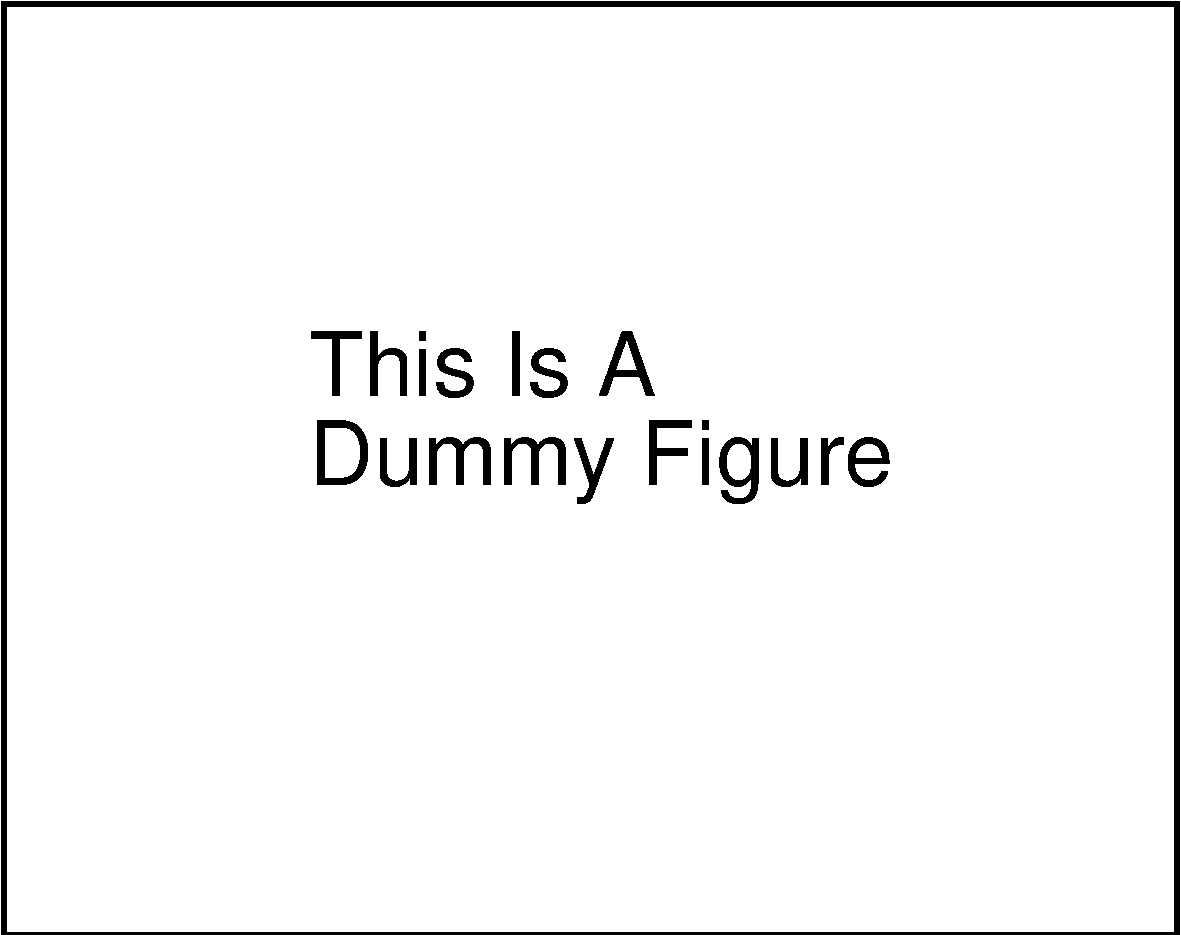
\includegraphics[width=\textwidth]{graphics/dummy.pdf}
}
\caption[Regions of nucleon-WIMP cross section versus WIMP
mass]{Regions of nucleon-WIMP scattering cross section (corresponding
  to dark matter in the lab moving with $v = 10^{-3}c$). The plot uses
  $m_V = 300$~MeV and $\alpha'=0.1$. Constraints are shown from
  different experiments.  The left plot shows the exclusion regions
  expected from MiniBooNE given 1-10 (light green), 10-1000 (green),
  and more than 1000 (dark green) elastic scattering events off
  nucleons. The right panel shows the same for elastic scattering off
  electrons. The magenta arrows indicate the region where DUNE can
  extend the MiniBooNE sensitivity. Figure is based on studies in ~\cite{Dharmapalan:2012xp}.}
\label{fig:wimp}
\end{figure}
If the DUNE ND were a LArTPC and the entire
detector volume active, the effective number of DM events detected
would be much higher when compared to a MINOS-like detector of the
same mass. Much more thorough studies must be conducted to obtain
reliable sensitivities. This requires an integration of theoretical
predictions into a simulation package for the detector.
% References for this section
% \bibitem{BATELL09} B. Batell, M. Pospelov and A. Ritz, ``Exploring Portals
%   to a Hidden Sector Through Fixed Targets,'' Phys. Rev. D 80,
%   095024 (2009), [arXiv:0906.5614 [hep-ph]].
% \bibitem{DENIVER11} P. deNiverville, M. Pospelov and A. Ritz,
%   ``Observing a light dark matter beam with neutrino experiments,''
%   Phys. Rev. D 84, 075020 (2011), [arXiv:1107.4580 [hep-ph]].
% \bibitem{DENIVER12} P deNiverville, D. McKeen and A. Ritz,
%   ``Signatures of sub-GeV dark matter beams at neutrino
%   experiments,'' Phys. Rev. D 86, 035022 (2012), [arXiv:1205.3499
%   [hep-ph]].
% \bibitem{DHARMAPALAN} R. Dharmapalan et al.  [MiniBooNE
%   Collaboration], ``Low Mass WIMP Searches with a Neutrino
%   Experiment: A Proposal for Further MiniBooNE Running,''
%   arXiv:1211.2258 [hep-ex].
% \bibitem{CERRILI05} M. Cirelli, N. Fornengo, T. Montaruli,
%   I. A. Sokalski, A. Strumia and F. Vissani, ``Spectra of neutrinos
%   from dark matter annihilations,'' Nucl. Phys. B 727, 99 (2005)
%   [Erratum-ibid. B 790, 338 (2008)], [hep-ph/0506298]
% \bibitem{AARTSEN13} M. G. Aartsen et al.  [IceCube Collaboration],
%   ``Search for dark matter annihilations in the Sun with the
%   79-string IceCube detector,'' Phys. Rev. Lett. 110, 131302
%   (2013)[arXiv:1212.4097 [astro-ph.HE]].

This section describes the current design and expected performance of the magnetized multi-purpose detector (\dword{mpd}), which is the downstream component of the \dword{dune}  \dword{nd} suite.

The \dword{mpd} consists of a high-pressure (10~bar) gaseous argon time projection chamber (\dword{hpgtpc}), surrounded by an \dword{ecal}, all situated inside of a dipole magnetic field provided by a superconducting magnet. A muon system is situated at the downstream end of the \dword{mpd}. The combined systems of the \dword{mpd} will provide tracking and charge-sign identification for particles exiting the downstream face of the \dword{arcube} \dword{lartpc}, and facilitate the associated constraints on the long-baseline oscillation analysis. As a stand-alone device, the \dword{mpd} will also collect independent event samples of neutrino interactions on argon, where the \dword{hpgtpc}'s lower density relative to a \dword{lartpc} will provide the opportunity to study in unprecedented detail the particles exiting the neutrino interaction vertices.


\subsection{High-Pressure Gaseous Argon TPC}
The basic geometry of the \dword{hpgtpc} is a gas-filled cylinder with a \dword{hv} electrode at its mid-plane, providing the drift \efield for ionization electrons. It is oriented inside the magnet such that the magnetic and electric fields are parallel, reducing transverse diffusion to give better point resolution. Primary ionization electrons drift to the end plates of the cylinder, which are instrumented with  to initiate avalanches (gas gain) at the anode wires.  Signals proportional to the avalanches are induced on cathode pads situated behind the wires; readout of the induced pad signals provides the hit coordinates in two dimensions.  The drift time provides the third coordinate of the hit.

The details of the \dword{hpgtpc} design will be based closely on the design of the ALICE detector~\cite{Dellacasa:2000bm} shown in Figure~\ref{fig:ALICETPC}. Two readout planes sandwich a central \dword{hv} electrode (25~$\mu$m of aluminized mylar) at high voltage that generates the drift field, which is parallel to a \SI{0.5}{T} magnetic field. On each side of the electrode, primary ionization electrons drift up to \SI{2.5}{m} to reach the endplates, which are segmented azimuthally into 18 trapezoidal regions and instrumented with \dwords{roc} that consist of \dwords{mwpc} amplification regions and cathode pad planes to read out the signals. A cross sectional view of an ALICE \dword{mwpc}-based \dwords{roc} is shown in Figure~\ref{fig:ALICE_ROC_MWPC}. The \dwords{roc} are built in two sizes: a smaller \dword{iroc} and a larger \dword{oroc}. The trapezoidal segments of the endplates are divided radially into inner and outer sections, and the \dwords{iroc} and \dwords{oroc} are installed in those sections. The existing \dwords{iroc} and \dwords{oroc} will become available in 2019, when they are scheduled to be replaced by new GEM-based \dwords{roc} for upgraded pileup capability in the high rate environment of the LHC. For the \dword{dune} \dword{hpgtpc}, the existing \dwords{roc} are more than capable of providing the necessary performance in a neutrino beam.  

%====================
\begin{figure}[h]
    \centering
    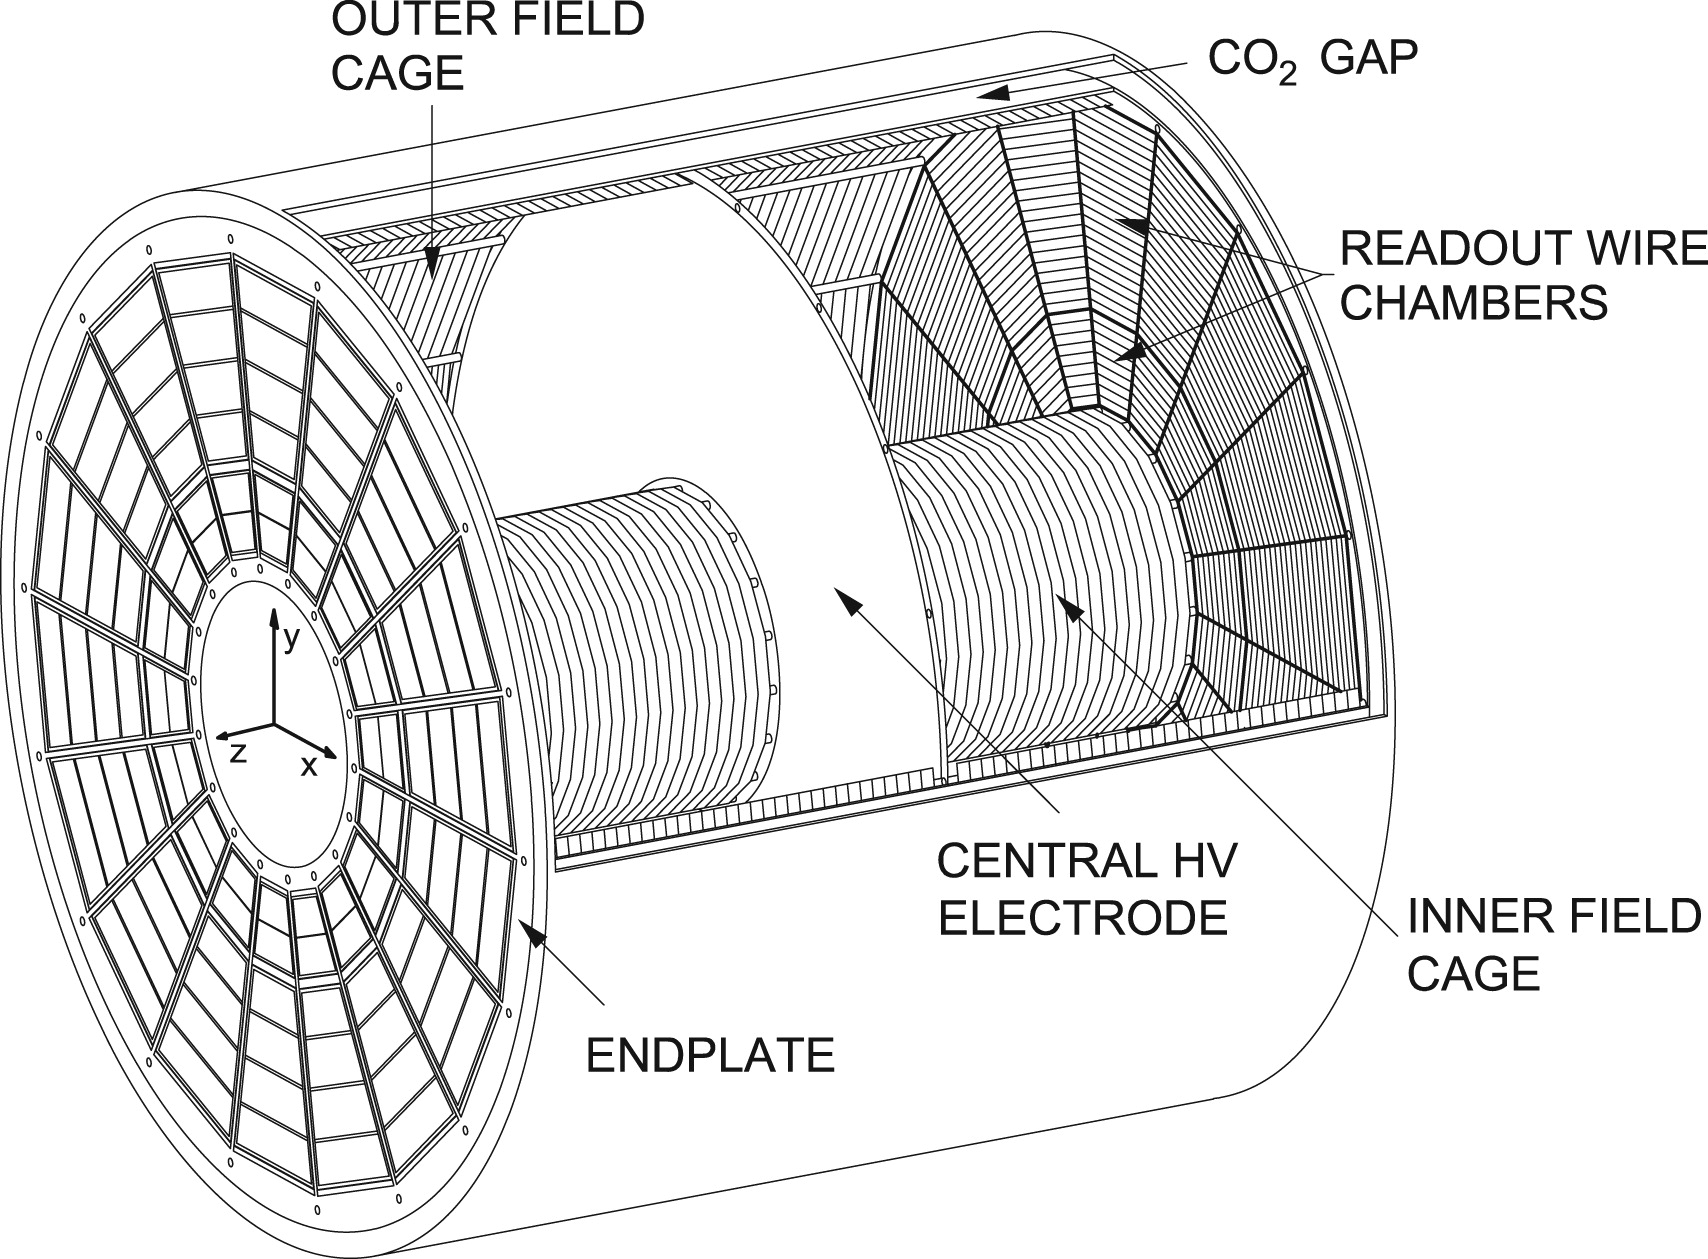
\includegraphics[width=0.8\textwidth]{graphics/alice_tpc_highres.jpg}
    \caption{Diagram of the ALICE TPC, from Ref.~\cite{Alme:2010ke}. The drift \dword{hv} electrode is located at the center of the \dword{tpc}, defining two drift volumes, each with 2.5~m of drift along the axis of the cylinder toward the endplate. The endplates are divided into 18 sectors, and each endplate holds 36 readout chambers.}
    \label{fig:ALICETPC}
\end{figure}
%====================


%====================
\begin{figure}[h]
    \centering
    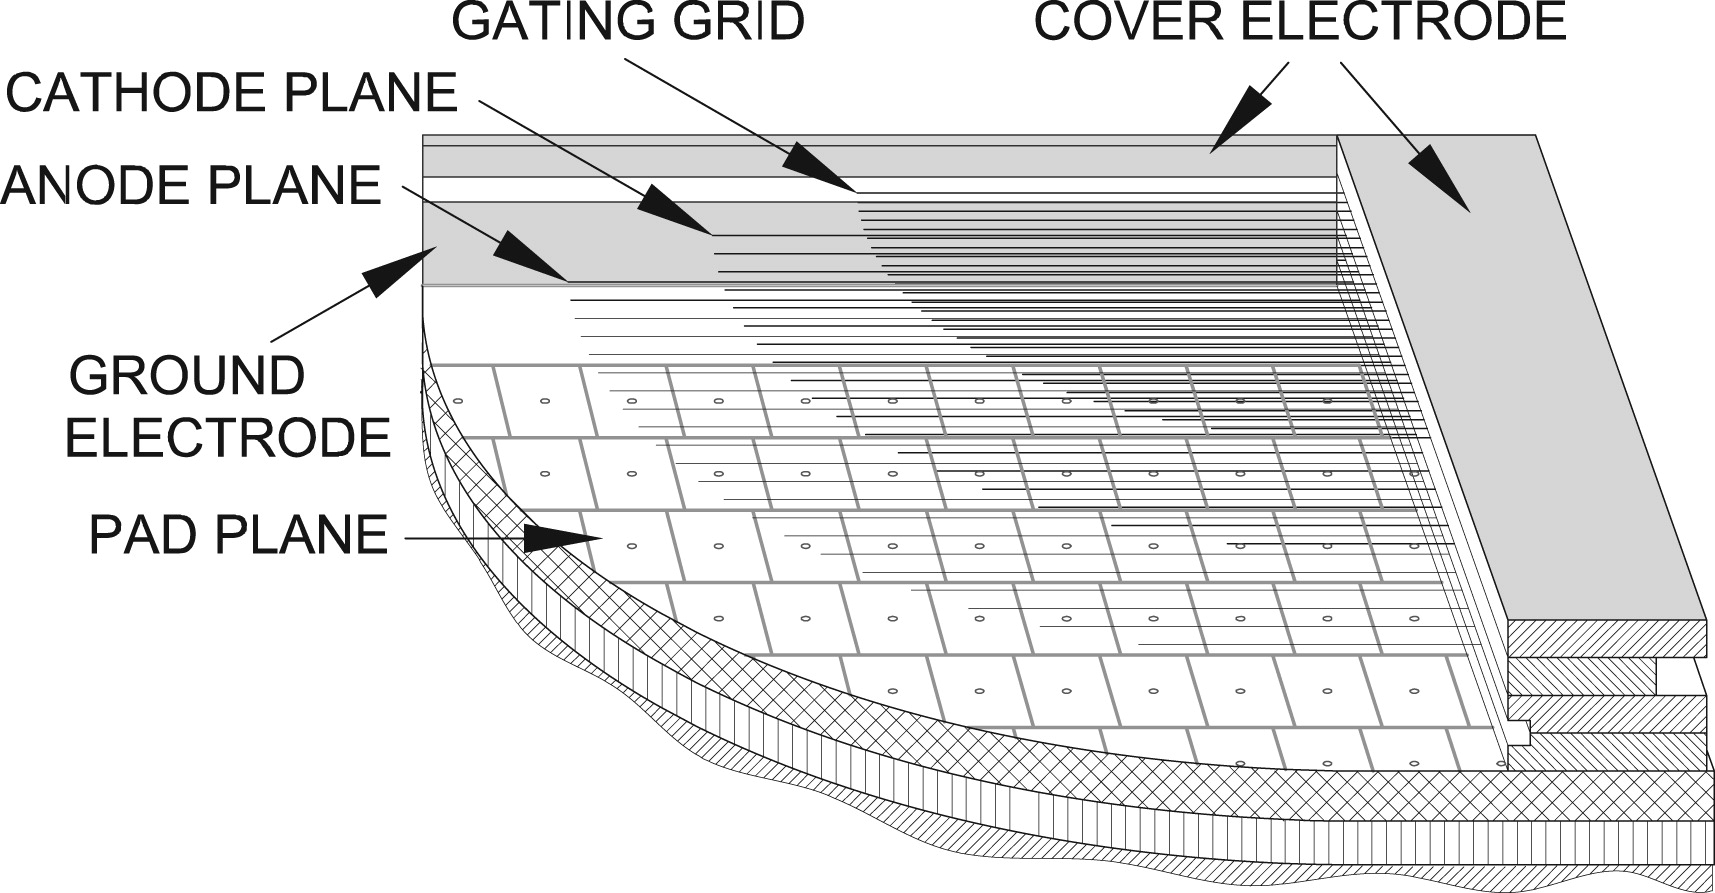
\includegraphics{graphics/TPC_ROC_MWPC.jpg}
    \caption{Schematic diagram of the ALICE \dword{mwpc}-based ROC with pad plane readout, from Ref.~\cite{Alme:2010ke}.}
    \label{fig:ALICE_ROC_MWPC}
\end{figure}
%====================

In the ALICE design, the inner-most barrel region was isolated from the \dword{tpc} and instrumented with a silicon-based inner tracker; for the \dword{dune} \dword{hpgtpc}, the inner field cage labeled in Figure~\ref{fig:ALICETPC} will be removed, and the entire inner region will be combined to make a single gas volume for the \dword{tpc}. Two new circular \dwords{roc}, each approximately \SI{1.6}{m} in diameter, will be built to fill in the central uninstrumented region left by reusing the existing ALICE chambers.  The active dimensions of the \dword{hpgtpc} will be \SI{5.2}{m} in diameter and \SI{5}{m} long, which yields an active mass of $\simeq$ \SI{1.8}{t}. 

The expected performance of the \dword{mpd} is summarized in Table~\ref{tab:TPCperformance}. Details of the \dword{hpgtpc} performance are based upon experience from operation of the PEP-4~\cite{PEP4_results_Layter,PEP4_Stork,Madaras:1982cj} and ALICE~\cite{Alessandro:2006yt} time projection chambers. Performance of the \dword{ecal} is based on experience from operation of similar \dwords{ecal} and on simulations. 

\begin{table}[h]
    \centering
    \caption{Expected \dword{mpd} performance}
\begin{tabular}{l|c|c}
\hline
Parameter	               & Value	                      & units \\
\hline
$\sigma_x$ 		           & 250	                      & $\mu$m\\
$\sigma_y$ 		           & 250	                      & $\mu$m\\
$\sigma_z$ 		           & 1500	                      & $\mu$m\\
$\sigma_{r\phi}$ 	       & <1000	                      & $\mu$m\\
Two-track separation       & 1		                      & cm \\
Angular resolution	       & 2-4	                      & mrad \\
$\sigma$($dE/dx$)		       & 5		                      & \% \\ 
$\sigma_{p_T}/p_T$	       & 0.7	                      & \% (10-1 GeV/c)\\
$\sigma_{p_T}/p_T$	       & 1-2	                      & \% (\SIrange{1}{0.1}{GeV/c})\\
Energy scale uncertaint    & $\lessapprox$ 1              & \% (dominated by $\delta_p/p$) \\
Charged particle detection thresh. & 5                    & MeV (K.E.)\\
\dword{ecal} resolution	           & 5-7/$\sqrt{E/{\rm{GeV}}}$	  & \% \\
\dword{ecal} pointing resolution &  $\simeq 6$ at 500 MeV         & degree\\ 
\hline\hline
\end{tabular} 
 \label{tab:TPCperformance}
\end{table}
%

\subsubsection{Track Reconstruction and Particle Identification}
Track reconstruction in ALICE is achieved by combining hits recorded on the ROC pads into tracks following a trajectory that a charged particle traveled through the \dword{tpc} drift volume. The ALICE offline \dword{tpc}-only track reconstruction performance is shown in Figure~\ref{fig:ALICE_offlinereco}. ALICE typically operates with particle densities ranging from 2000 to 8000 charged particles per unit rapidity ($dN/dy$) for central Pb-Pb interactions~\cite{Cheshkov:2006ym}, whereas such high particle densities will never be seen with this detector placed in any neutrino  \dword{nd} environment. 


\begin{figure}[h]
    \centering
    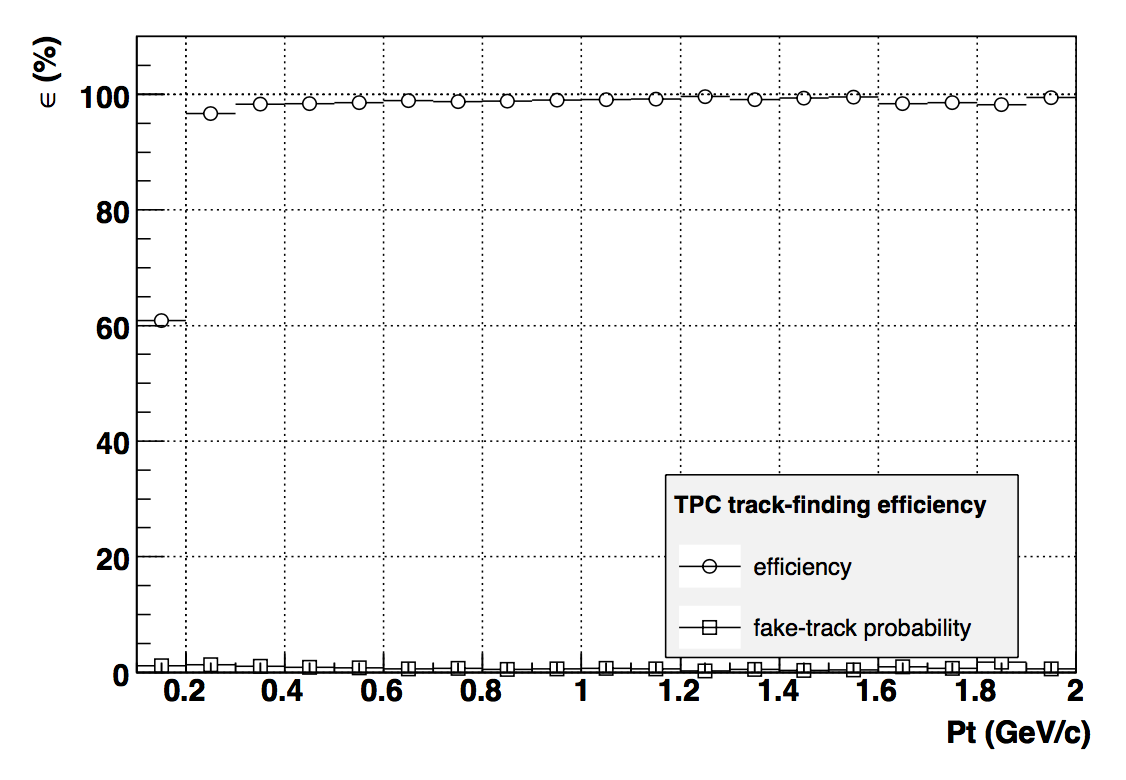
\includegraphics[width=0.6\textwidth]{graphics/ALICE_TPCreco.png}
    \caption{From Ref.~\cite{Alessandro:2006yt}. Efficiency of the ALICE \dword{tpc} track-finding software as a function of track transverse momentum for event multiplicity of 6000 tracks per unit of rapidity in Pb-Pb collisions (open circles), and corresponding fake track candidates (open squares).}     
    \label{fig:ALICE_offlinereco} 
\end{figure}

ALICE chose to use neon, rather than argon, for the primary gas; the decision was driven by a number of factors, but two-track separation capability was one of the primary motivations due to the extremely high track multiplicities in the experiment.  Neon performs better than argon in this regard.  A better comparison for the \dword{hpgtpc}'s operation in \dword{dune} is the two-track separation that was obtained in PEP4~\cite{PEP4_Stork}.  PEP4 ran an 80-20 mixture of Ar-CH$_4$ at 8.5~atmospheres, yielding a two-track separation performance of \SI{1}{cm}.

In ALICE, the ionization produced by charged particle tracks is sampled by the \dword{tpc} pad rows (there are 159 pad rows in the \dword{tpc}) and a truncated mean is used for the calculation of the PID signal. Figure~\ref{fig:ALICE_dEdx} (left) shows the ionization signals of charged particle tracks in ALICE for pp collisions at $\sqrt{s} = 7$~TeV. The different characteristic bands for various particles are clearly visible and distinct at momenta below a few GeV.  When repurposing ALICE as the \dword{hpgtpc} component of the \dword{mpd}, we expect even better performance for particles leaving the active volume, since the detector will be operating at higher pressure (10~Atm vs. the nominal ALICE 1~Atm operation), resulting in ten times more ionization per unit track length available for collection. Figure~\ref{fig:ALICE_dEdx} (right) shows the charged particle identification for PEP-4/9~\cite{Grupen:1999by}, a higher pressure gas \dword{tpc} that operated at 8.5~Atm pressure, which is very close to the gas mixture and pressure at which the \dword{hpgtpc} will be operated.

\begin{figure}[htb]
\centering 
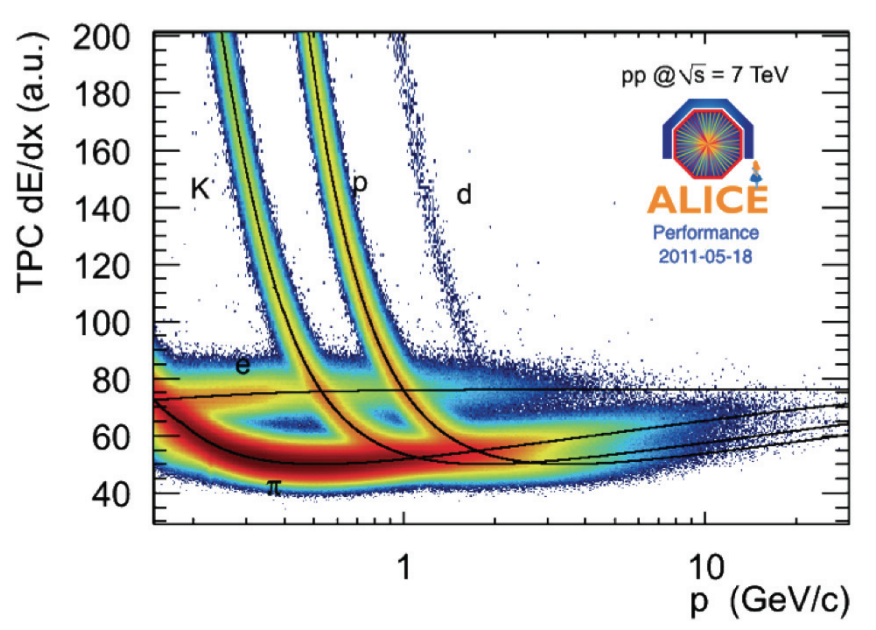
\includegraphics[width=0.49\textwidth]{graphics/ALICE_TPC_dEdx_Lippmann_2012.png}
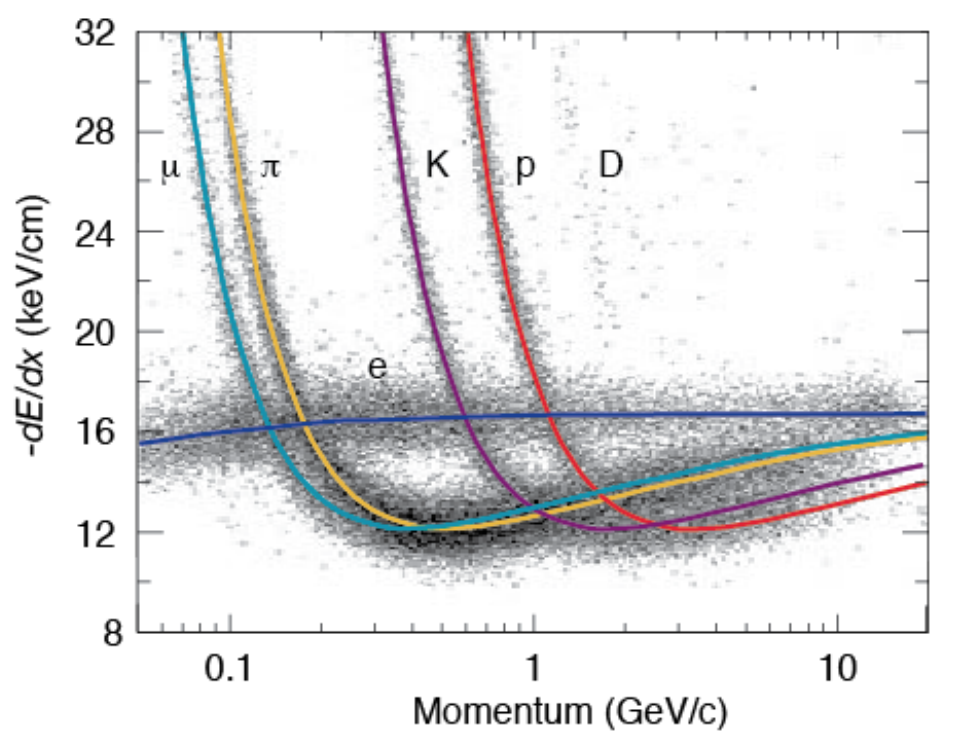
\includegraphics[width=0.49\textwidth]{graphics/PEP4-TPC-80Ar-20CH4-8_5atm_dEdx.png} 
\caption{Left: ALICE TPC dE/dx-based particle identification as a function of momentum (from~\cite{ALICE_Lippmann}). Right: PEP-4/9 TPC (80:20 Ar-CH4, operated at 8.5~Atm, from~\cite{Grupen:1999by}) dE/dx-based particle identification.} 
\label{fig:ALICE_dEdx} 
\end{figure}

\subsubsection{Momentum and Angular Resolution for Charged Particles}
%
The ability to determine the sign of a charged particle in the \dword{tpc} tracking volume is limited by the spatial resolution of the measured drift points in the plane perpendicular to the magnetic field, as well as multiple Coulomb scattering (MCS) in the gas. However, for almost all tracks, MCS has a small effect on momentum or angular resolution in the \dword{hpgtpc}. For a fixed detector configuration, the visibility of the curvature depends on the particle's $p_{\rm{T}}$, the track length in the plane perpendicular to the field, and the number and closeness of nearby tracks.  Because primary vertices are distributed throughout the tracking volume, the distribution of the lengths of charged-particle tracks is expected to start at very short tracks, unless sufficient fiducial volume cuts are made to ensure enough active volume remains to determine particle's track sign.

Within the fiducial volume of the \dword{hpgtpc}, charged-particles can be tracked over the full 4$\pi$ solid angle.  Even near the central electrode,  tracking performance will not be degraded due to the very thin (25 $\mu$m of mylar) nature of the central electrode.  The 4$\pi$ coverage is true for all charged particles.  ALICE ran with a central field of 0.5~T and their momentum resolution from p--Pb data~\cite{Abelev:2014ffa} is shown in Figure~\ref{fig:ALICE_MOMres}.

\begin{figure}[h]
\centering 
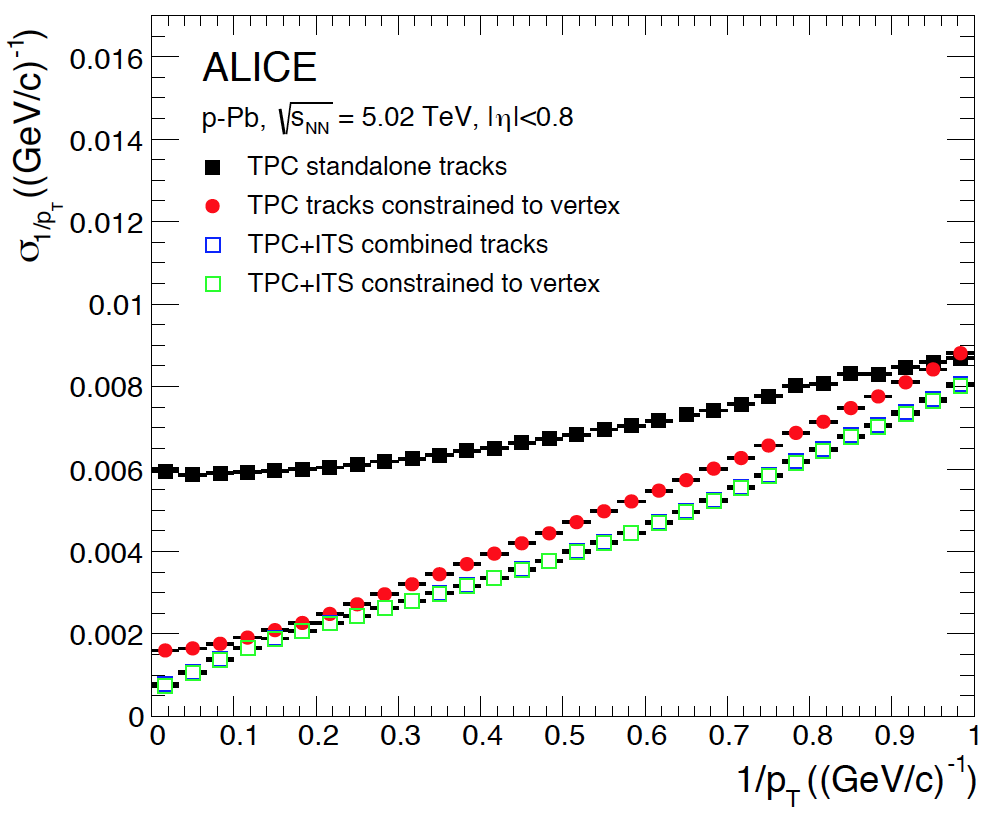
\includegraphics[width=0.85\columnwidth]{graphics/ALICE_mom_res.png} 
\caption{The black squares show the TPC stand-alone p$_T$ resolution in ALICE for p--Pb collisions. From Ref.~\cite{Abelev:2014ffa}.} 
\label{fig:ALICE_MOMres} 
\end{figure}

\subsubsection{MPD Pressure Vessel}\label{sec:TPC_PV}

The preliminary design of the pressure vessel, presented in Figure~\ref{fig:TPC_PV}, accounts for the additional volume needed to accommodate the \dword{tpc} field cage, the ROC support structure, front-end electronics, and at least part of the \dword{ecal}.

The pressure vessel is fabricated from stainless steel, has a cylindrical section that is 6~m in diameter and 6~m long and utilizes two semi-elliptical end pieces with flanges. The walls of the cylinder barrel section are $\simeq$~1.6X$_0$ in thickness.  Further reduction of the thickness in radiation lengths can be accomplished with a change in material (Ti) or with the addition of stiffening rings.  The vessel is rated for 175~psia.  While the preliminary design includes flanged endcaps, the cost of flanging is significant, and therefore vessel designs with a single flange or with a fully-welded vessel will also be considered.  

%====================
\begin{figure}[ht]
\centering 
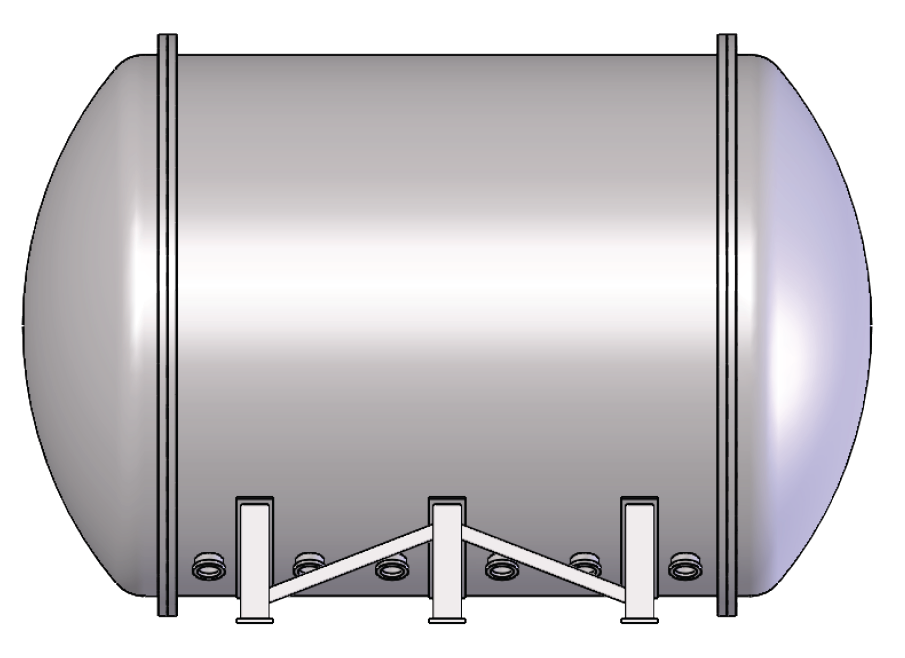
\includegraphics[width=0.75\textwidth]{graphics/tpc_pressurevessel.png} 
\caption{Pressure vessel preliminary design} 
\label{fig:TPC_PV} 
\end{figure}
%====================

\subsection{Electromagnetic Calorimeter}
%The \dword{dune} Near detector has been designed as a multi-purpose detector. A high-pressure gas Time Projection Chamber followed by a calorimeter system. The complete system is located within a \SI{0.4}{\tesla} coil. 
The \dword{nd} \dword{ecal} concept is based on a high granularity calorimeter to provide direction information in addition to the energy measurement of electromagnetic showers and an efficient rejection of background.

The principal role of the \dword{ecal} is to reconstruct photons directly produced in $\nu$ interactions and originating from $\pi^0$ decays, providing a measurement of the photon's energy and direction to enable the association of photons to interactions observed in the \dword{hpgtpc} and the determination of the decay vertex of the $\pi^0$s. The \dword{ecal} can also be used to reject backgrounds, such as rock neutrons and muons, providing a sub-nanosecond timestamp \cite{Simon:2013zya} for each hits in the detector. As the \dword{ecal} uses hydrogen-rich scintillator, it is assumed to have capabilities to provide neutron detection.

\subsubsection{ECAL Design}

The \dword{ecal} design is inspired by the design of the CALICE Analog Hadron Calorimeter (AHCAL) \cite{collaboration:2010hb} developed within the CALICE collaboration \cite{CALICEwebsite}.
\begin{dunefigure}[Conceptual design of the \dword{ecal} for the Near Detector.]{fig:ConceptDesign_NDECAL}
{On the left, the conceptual design of the \dword{hpgtpc} + \dword{ecal} barrel system for the Near Detector. The full \dword{ecal} is located inside the \dword{hpgtpc} pressure vessel. On the right, a conceptual design of the \dword{ecal} endcap system.}
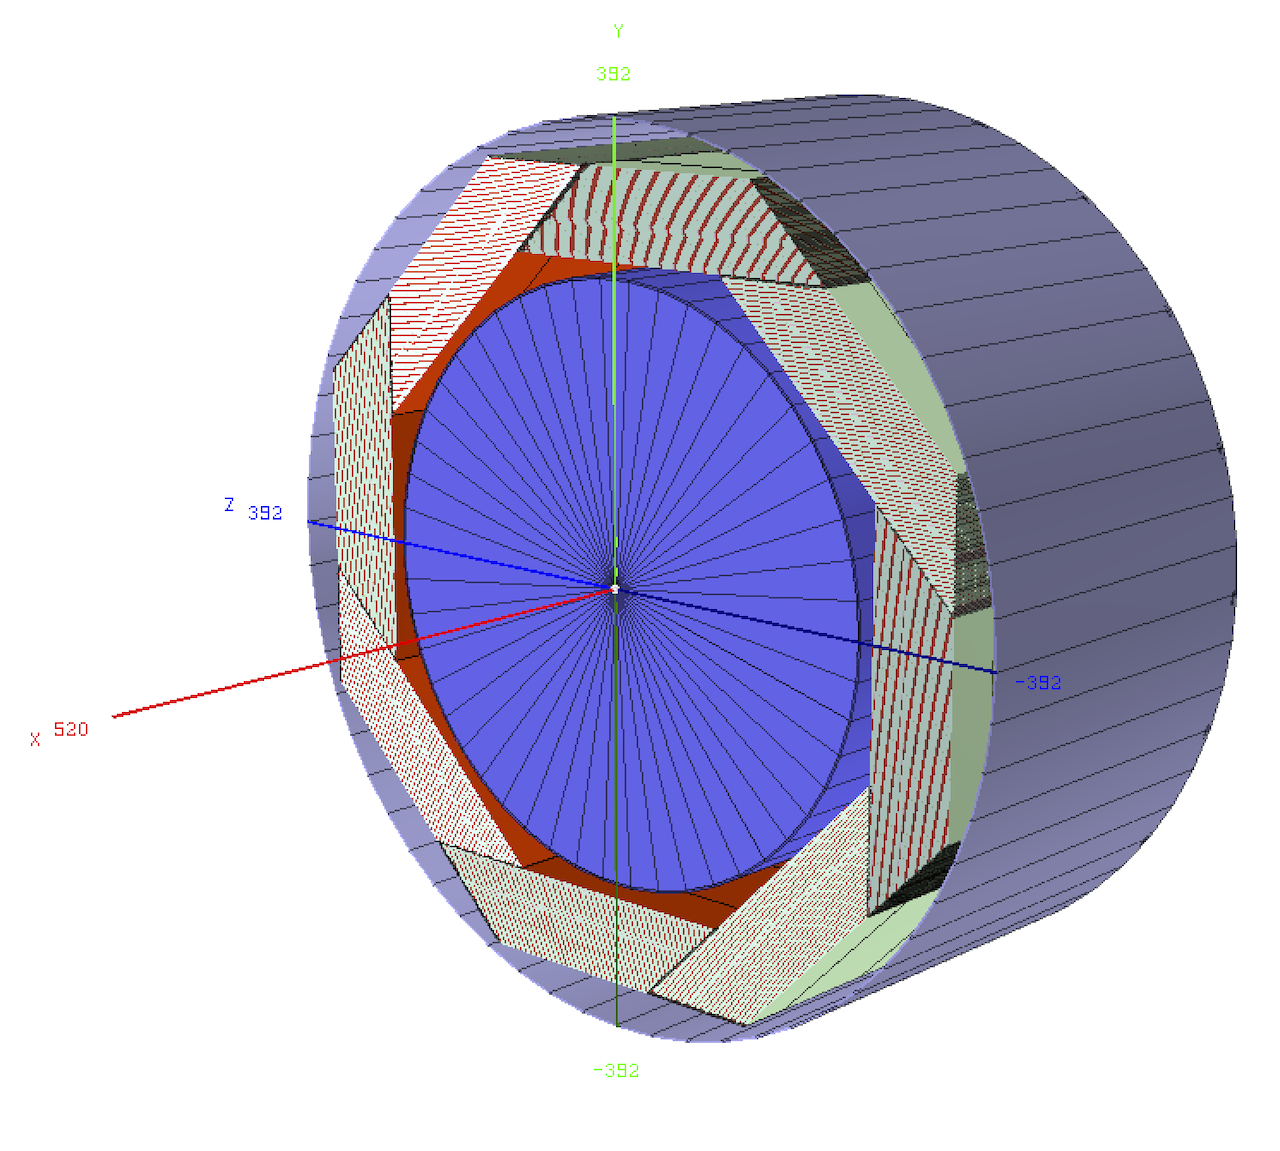
\includegraphics[width=0.45\textwidth]{graphics/ConceptECALND.png}
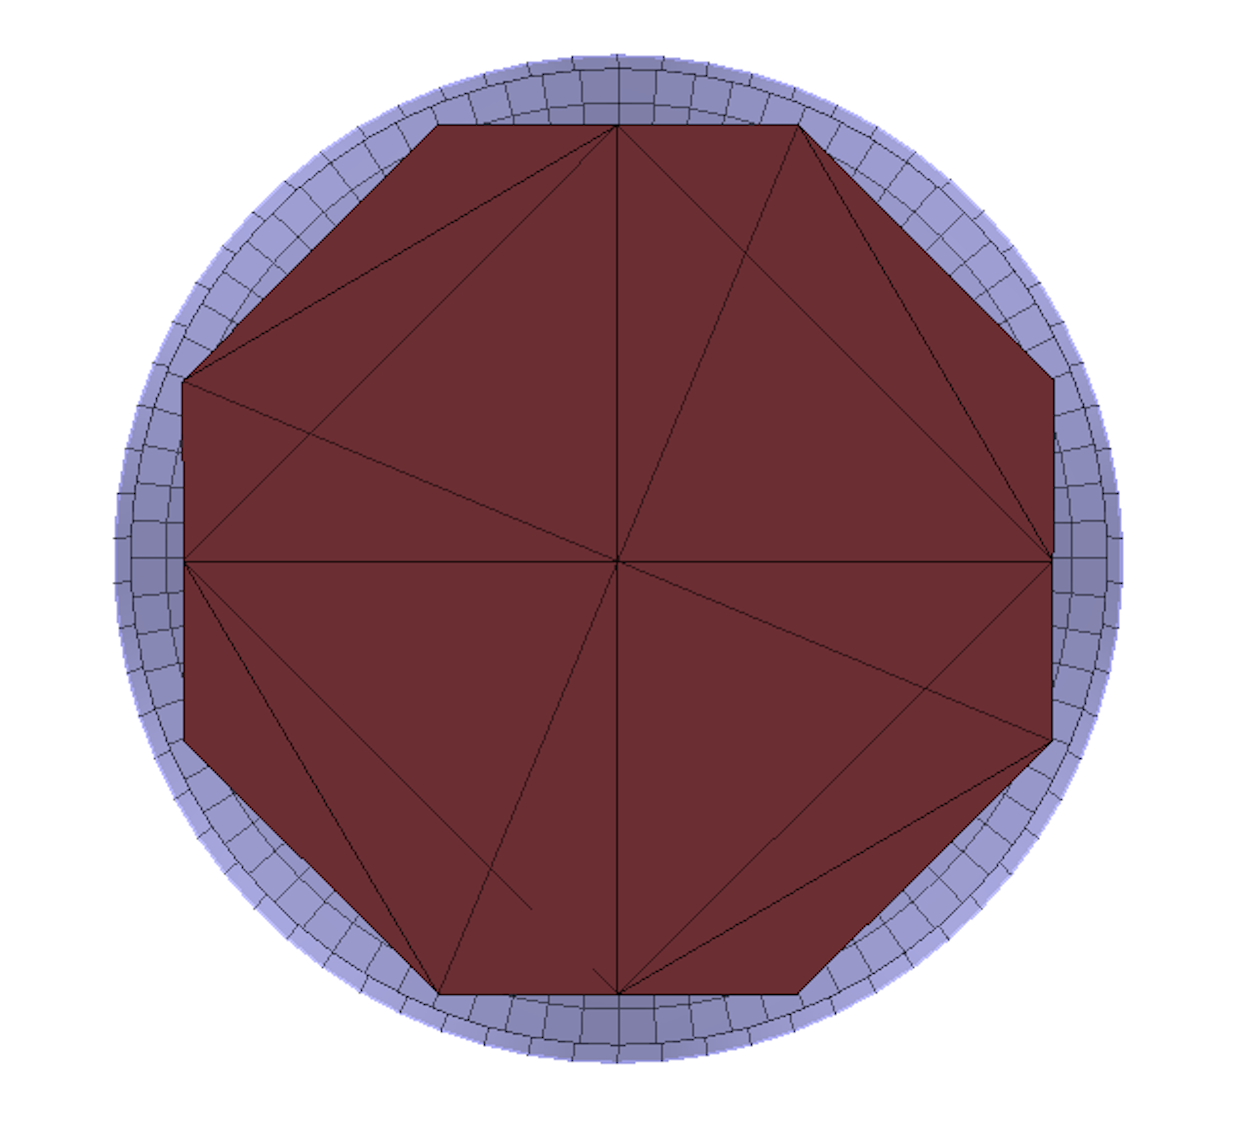
\includegraphics[width=0.42\textwidth]{graphics/ECAL_Endcap_System.png}
\end{dunefigure}
As shown in figure \ref{fig:ConceptDesign_NDECAL}, the \dword{ecal} Barrel has an octagonal shape, each quadrant composed of several trapezoidal modules. The \dword{ecal} end-cap has a similar design providing hermeticity and a large solid-angle coverage. Each module consists of scintillating layers of polystyrene as active material readout by silicon-photomultipliers, sandwiched between absorber sheets. The scintillating layers consist of a mix of tiles with dimensions between $2\times2$ cm$^2$ to $3\times3$ cm$^2$ (see Figure \ref{fig:ConceptTile_NDECAL}) and cross-strips with embedded wavelength shifting fibers to achieve a comparable effective granularity. The high granularity layers are concentrated in the front part of the detector since it has been shown to be the most relevant factor for the angular resolution \cite{Emberger:2018pgr}. With the current design, the number of channels is in the order 2.5 to 3 million. A first design of the \dword{ecal} and the simulated performance has already been studied in \cite{Emberger:2018pgr}.

\begin{dunefigure}[Conceptual layout of the calorimeter.]{fig:ConceptTile_NDECAL}
  {Conceptual layout of the calorimeter showing the absorber structure, scintillator tiles, SiPM and PCB.}
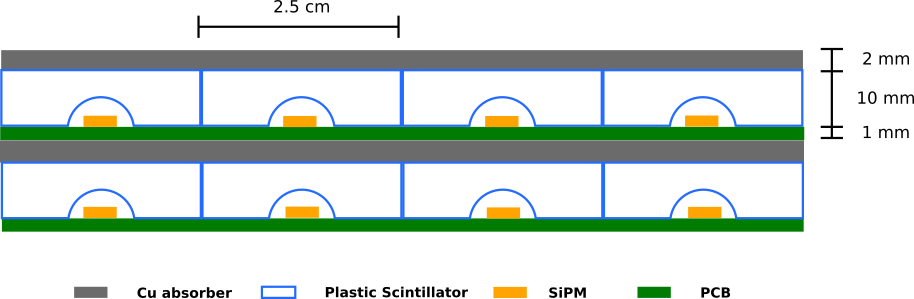
\includegraphics[width=0.8\textwidth]{graphics/TileConcept.png}
\end{dunefigure}

One major design driver is the pressure vessel limiting the space. Therefore, a compact calorimeter is needed. It is assumed that either the full \dword{ecal} barrel can be fit inside the pressure vessel or that it will consist of two segments, one inside and one outside the pressure vessel. The first option is preferred to reduce the impact of the pressure vessel on the calorimeter energy resolution \cite{Emberger:2018pgr}. Currently, the \dword{ecal} design is going through a detailed design study in order to further optimize the detector design and performance.

\subsubsection{Simulated ECAL Performance}

The expected performance of the calorimeter was studied with Geant4-based \cite{Agostinelli:2002hh} simulations and GArSoft \cite{GArSoftwebsite}, a software based on the art framework \cite{ARTwebsite} and LArSoft \cite{Snider:2017wjd} developed specifically for the \dword{hpgtpc}. In the following, a first scenario referred to as scenario A (shown by the red curve in the figures below) in which the \dword{ecal} is within the pressure vessel is considered. The barrel geometry consists of 55 layers with the following layout:
\begin{itemize}
  \item 8 layers of \SI{2}{\mm} copper + \SI{10}{\mm} of $2.5\times2.5$ cm$^2$ tiles + \SI{1}{\mm} FR4
  \item 47 layers of \SI{4}{\mm} copper + \SI{10}{\mm} of cross-strips \SI{4}{\cm} wide
\end{itemize}
For the present studies, copper has been chosen as absorber material as first studies have shown that this material provides a good compromise between calorimeter compactness, energy resolution and angular resolution. However, the choice of absorber material is still under study. The choice of granularity, scintillator thickness and the arrangement of tiles and strips is still under optimization in order to reduce the number of readout channels while keeping the calorimeter performance. Two alternative scenarios are shown below, with a different arrangement of the tile and strip layers refered a scenario B (black curve) and with thinner absorbers in the front layers referred a scenario C (blue curve).
Digitization effects are accounted for by introducing an energy threshold of 0.25 MIPs ($\sim$\SI{200}{\keV}) for each detector cell/strip, a Gaussian smearing of \SI{0.1}{\MeV} for the electronic noise, SiPM saturation effects and single photon statistics.

\textbf{Energy Resolution} The energy resolution is determined by fitting the visible energy with a Gaussian fit. Converted photons are rejected based on Monte-Carlo information. A fit function of the form $\frac{\sigma_{E}}{E} = \frac{A}{\sqrt{E}} \oplus \frac{B}{E} \oplus C$ is used, A denotes the stochastic term, B the noise term and C the constant term. Figure \ref{fig:EResARes_NDECAL} shows the energy resolution as a function of the photon energy. For scenario A, shown in red, the energy resolution is around $\frac{6.7\%}{\sqrt{E}}$. With further optimization, it is believed that an energy resolution of (or below) $\frac{6\%}{\sqrt{E}}$ is achievable. It should be noted that due to the lack of non-uniformities, dead cells and other effects in the simulation, the energy resolution is slightly optimistic.

\begin{dunefigure}[Energy resolution and angular resolution in the barrel as a function of the photon energy.]{fig:EResARes_NDECAL}
{On the left, the energy resolution in the barrel as a function of the photon energy for three \dword{ecal} models. The energy resolution is determined by a Gaussian fit to the visible energy. On the right, the angular resolution in the Barrel as a function of the photon energy for three \dword{ecal} models. The angular resolution determined by a Gaussian fit to the 68\% quantile distribution. For both figures, the scenario A is shown by the red curve, scenario B by the black curve and scenario C by the blue curve. The fit function is of the form $\frac{\sigma_{E}}{E} = \frac{A}{\sqrt{E}} \oplus \frac{B}{E} \oplus C$.}
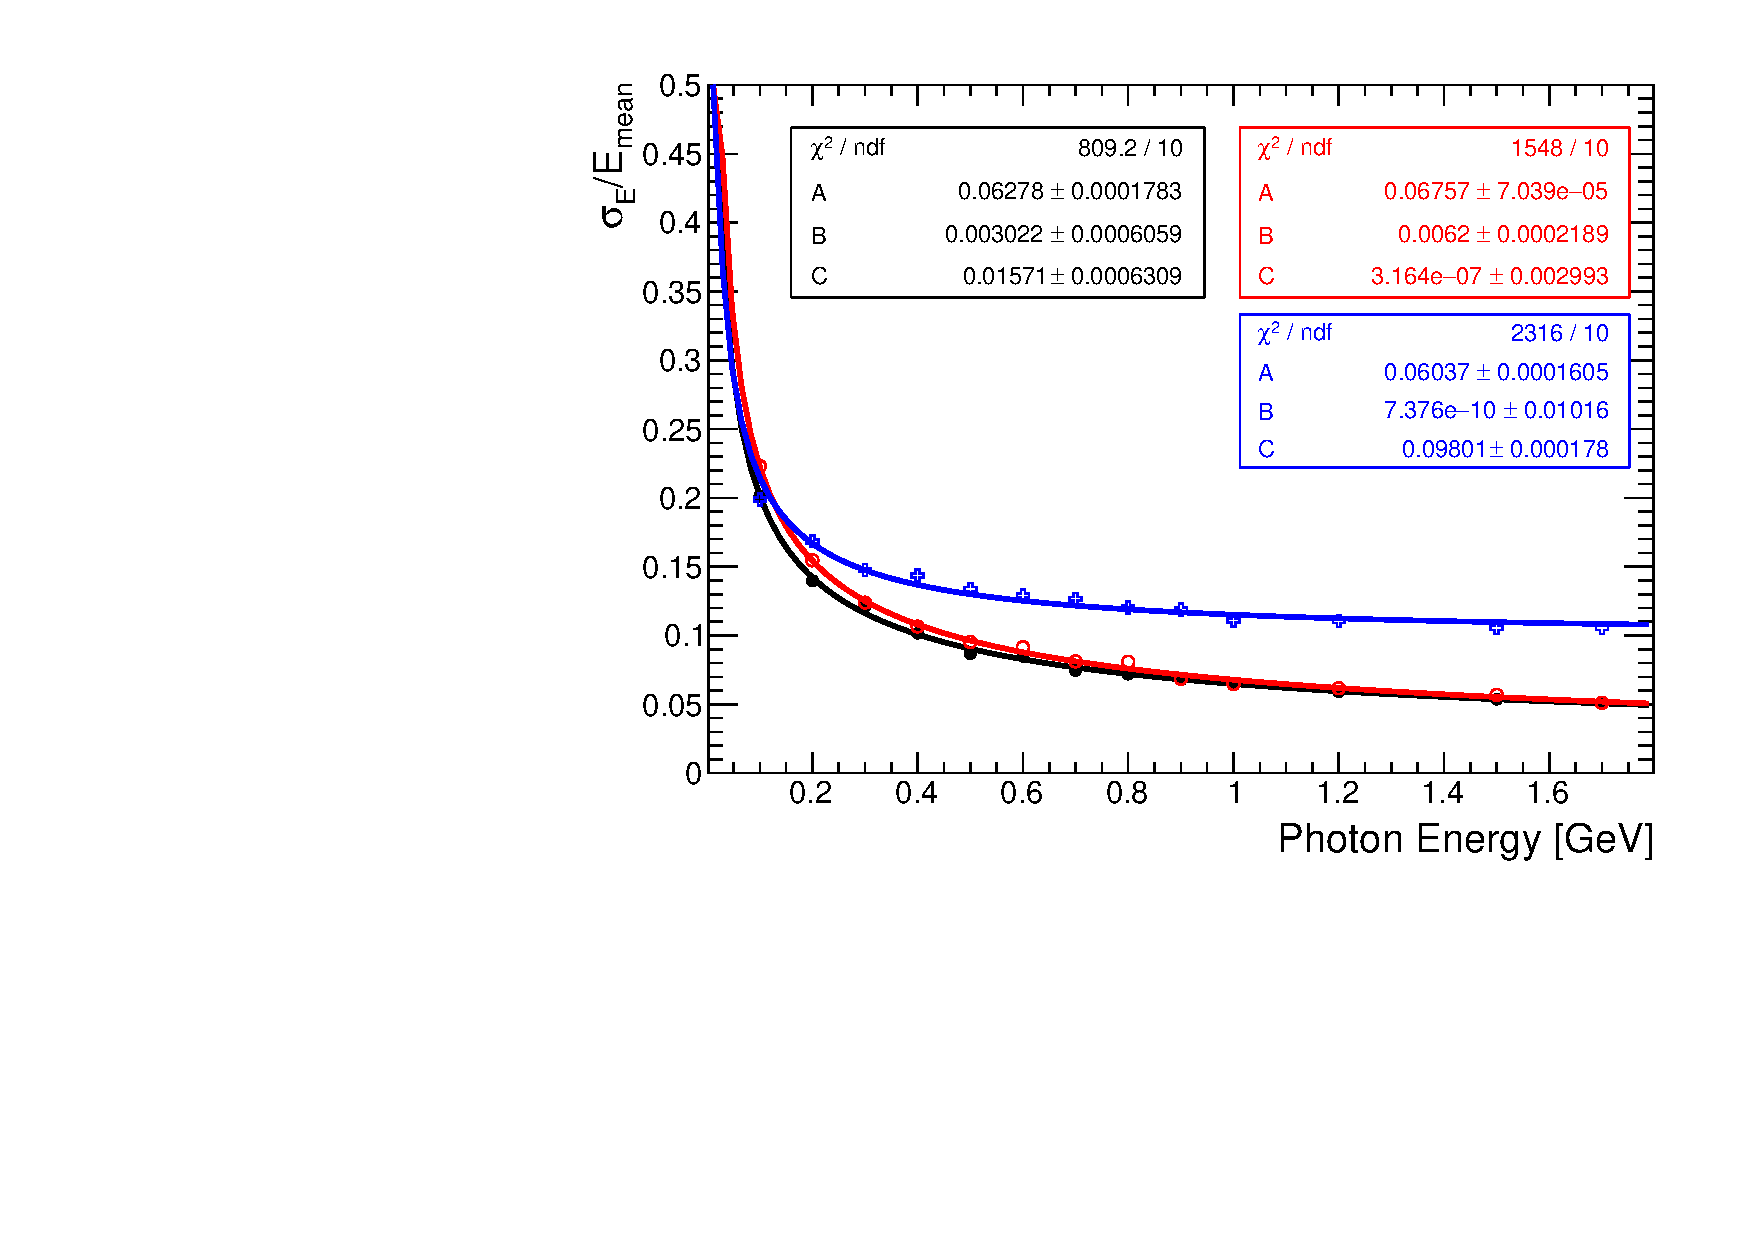
\includegraphics[width=0.45\textwidth]{graphics/Comparison_Setups_EnergyResolution.pdf}
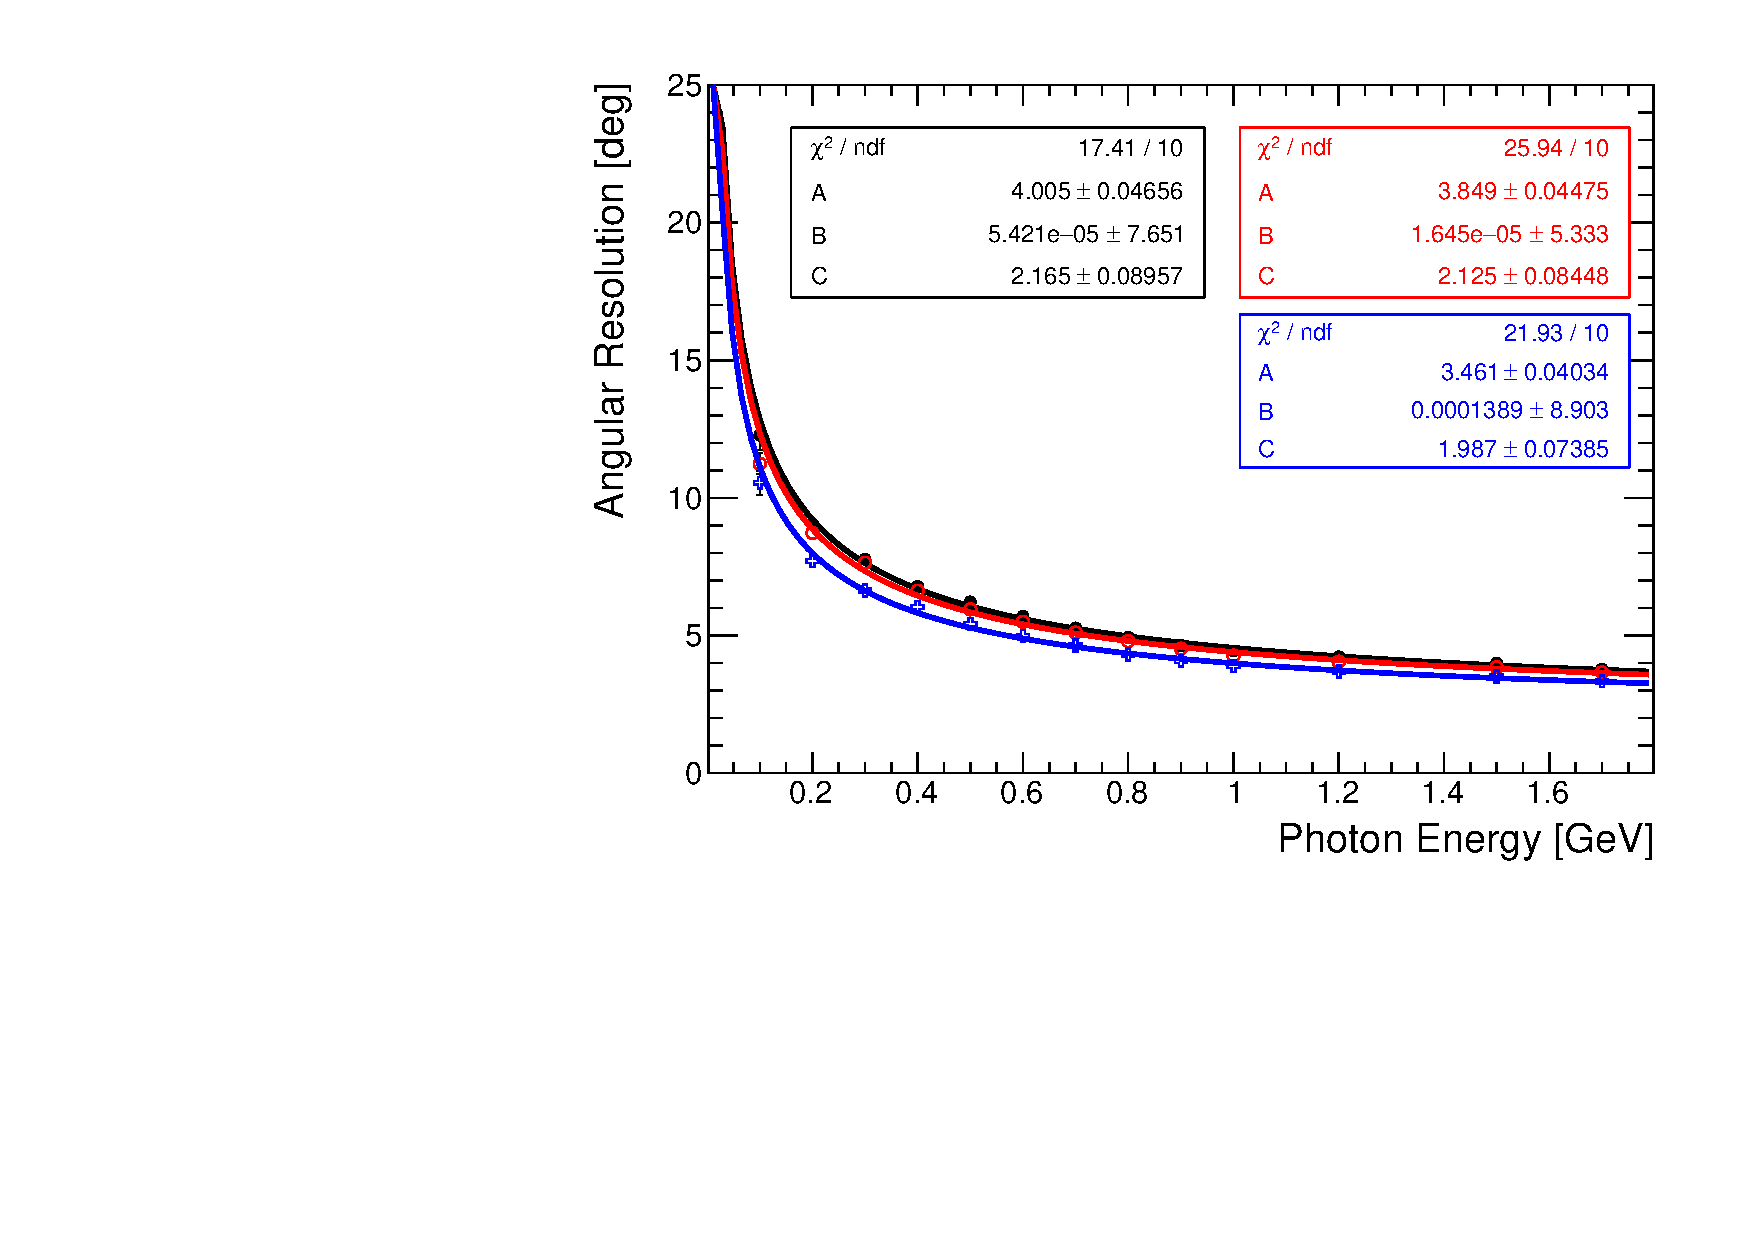
\includegraphics[width=0.45\textwidth]{graphics/Comparison_Setups_AngularResolution.pdf}
\end{dunefigure}


\textbf{Angular Resolution} The angular resolution of the calorimeter has been determined using a principal component analysis (PCA) of all reconstructed calorimeter hits. The direction is taken as the first eigenvector (main axis) of all the reconstructed hits. The angular resolution is determined by taking the 68\% quantile of the reconstructed angle distribution and fitting a Gaussian distribution. The mean is the Gaussian is taken as the angular resolution and the error as its variance. Figure \ref{fig:EResARes_NDECAL} shows the angular resolution as a function of the photon energy. With the scenario A showed in red, an angular resolution of $\frac{\SI{3.85}{\degree}}{\sqrt{E}} \oplus \SI{2.12}{\degree}$ can be achieved. This can potentially be further improved with a different arrangement of the tile and strip layers, an optimization of the absorber thickness and the reconstruction method in order to achieve an angular resolution better by a factor of around two compared to \dword{t2k} \cite{Abe:2011ks, Guzowski:2011duw} for energies below \SI{1}{\GeV}. However, the requirements will be further refined and will impact the detector optimization. The angular resolution is mainly driven by the energy deposits in the first layers of the ECAL. Using an absorber with a large $X_{0}$ creates an elongated shower that helps in determining the direction of the shower. In general, a high granularity leads to a better angular resolution, however, studies have shown that there is no benefits for cell sizes below $2\times2$ cm$^2$ \cite{Emberger:2018pgr}.



\textbf{Neutron detection} The \dword{ecal} is sensitive to neutrons due to the scintillator containing hydrogen. Previous simulation studies showed that a detection efficiency above 60\% can be achieved for neutron energies greater than \SI{50}{\MeV}. However, the energy measurement is not very accurate (around 50-60\% below \SI{600}{\MeV}) \cite{Emberger:2018pgr}. Other methods of detection such as Time of Flight (ToF) could be used to improve the neutron energy measurement by measuring precisely the hit time of the neutron and its travel distance in the calorimeter.  This is under study.

\textbf{$\pi^0$ reconstruction} For identification of neutral pions, both the energy and angular resolution are relevant. In a first study, the position of the neutral pion is determined by using a $\chi^2$-minimization procedure taking into account the reconstructed energy of the two photons and the reconstructed direction of the photon showers \cite{Emberger:2018pgr}. The location of the decay vertex of the neutral pion can be determined with an accuracy between \SIrange{10}{40}{\cm}, depending on the distance from the downstream calorimeter and the $\pi^0$ kinetic energy. This should be sufficient  to associate the $\pi^0$ to an interaction in the \dword{hpgtpc}. 
%However, this study needs to be reviewed again with the new design. 
This may be further improved by a more sophisticated analysis technique and by using precision time information, and is a subject of current study.




\subsection{Magnet}
%\subsection{Introduction}
%
Two magnet designs are under consideration to house the high pressure gas TPC and the ECAL. One is a UA1-type electromagnet, the other is based on a superconducting Helmholtz-coil like design. The common requirement is a central magnetic field of 0.5\,T with $\pm$20\% uniformity over the TPC volume (5\,m long and 5\,m in diameter). With the current design of the access shaft (11.8\,m diameter), the clear diameter is about 7.8\,m. Recent studies for the construction of an electromagnet similar to the UA1 magnet predict that the cost of the design, procurement, infrastructure (power and cooling) and assembly will be in excess of \$20 million, with operation costs of approximately \$1.6M per year of running.  Because of this, the main focus has been on a superconducting design.
%
\subsubsection{Superconducting %(SC) 
Magnet}
\label{ssec:SCmagnet}
%
The SC magnet design is an Helmholtz coil-like configuration, air core,  five coil magnet system. Three central coils produce the analyzing field and two outer shielding coils help contain stray field. The advantage of this design is that little or no iron is used for field containment or shaping. This eliminates background coming from neutrino interactions in the iron, which for the normal-conducting magnet case is the largest component of the background. Figure~\ref{fig:dune_nd_magnet_sc_layout} shows the coil concept. All five coils have the same inner radius of 3.5\,m. The center and shielding coils are identical with the same number of ampere-turns. The side coils are placed at 2.5\,m, the shielding coils at 6\,m from the magnet center along Z.  The case where the shielding coils are at 5\,m from the magnet center so that the magnet system would be the same width as the \dword{lar} detector is also being examined.  The magnet system will have a stored energy of about 110MJ, using a conventional NbTi superconducting cable design, a SSC-type Rutherford cable soldered in a copper channel with a 50\% margin. All coils should be wired in series to reduce imbalanced forces during a possible quench. Possible small transverse centering force components are possible due to coil de-centering from mechanical errors. 
%
Shown in Figure~\ref{fig:dune_nd_magnet_sc_fieldmap} is the field along the Z-axis at different radii. The peak field in the coils is 2.14\,T (center), 5\,T (side) and 2.03\,T (shield). The resulting forces are only along the Z-axis, $F_{z}$ is 0.0\,MN (center), -6.81\,MN (side) and 2.2\,MN (shield). The fringe field at the shielding coil is rather large but can be reduced further; more studies will be needed. There is a preliminary mechanical support design. A first glimpse a the radiative heat load assumes a coil and support surface of 180\,m$^{2}$, resulting in a load of 5.4\,W from 77\,K to 4.5\, K. The coil support and leads will likely have a much larger contribution (HTS power leads usually have 15W for 10kA. With a mass of 42\,t the magnets are in some aspects similar to the Mu2e solenoids.
%
\begin{figure}[h] 
\centering
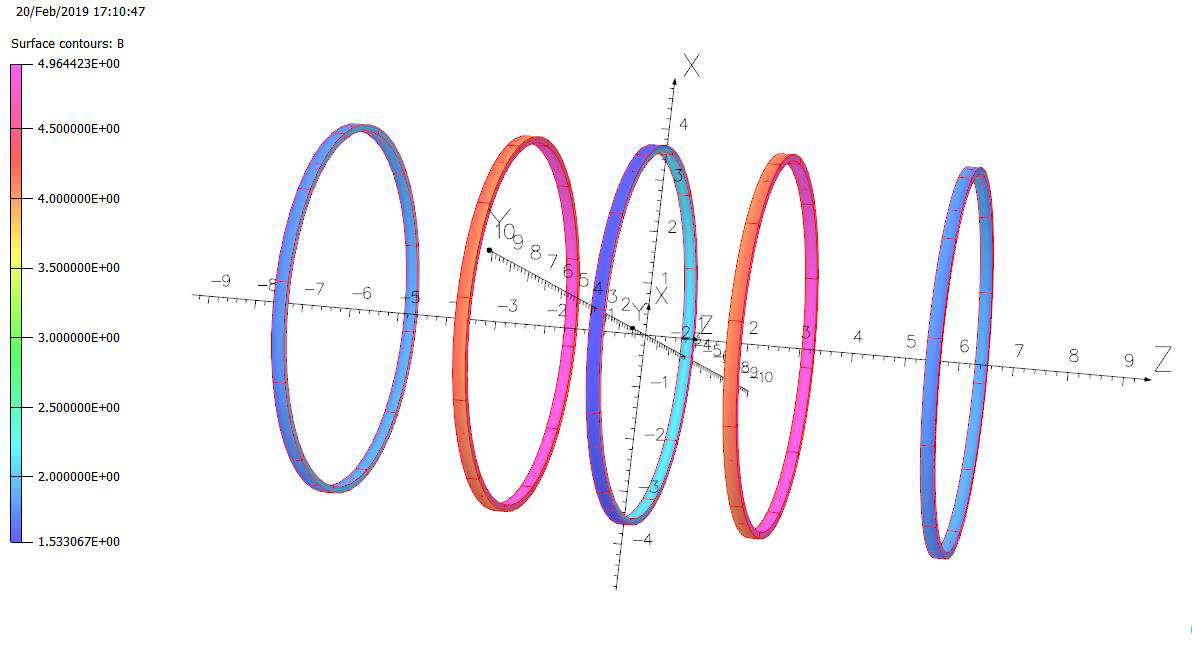
\includegraphics[width=0.95\columnwidth]{graphics/dune_nd_magnet_sc_layout.png} 
\caption{Helmholz coil arrangement.} 
\label{fig:dune_nd_magnet_sc_layout} 
\end{figure}
%
\begin{figure}[h] 
\centering
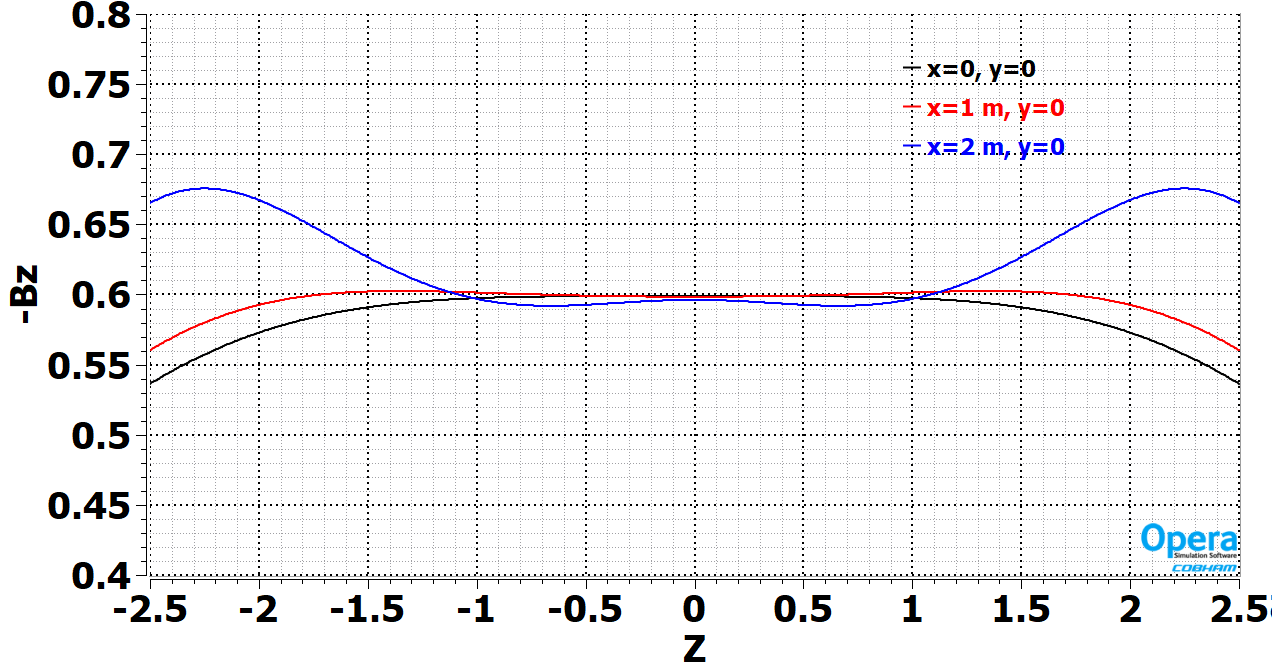
\includegraphics[width=0.95\columnwidth]{graphics/dune_nd_magnet_sc_fieldmap.png} 
\caption{Field Map along the Z-axis. The colors represent different radii from the center line.} 
\label{fig:dune_nd_magnet_sc_fieldmap} 
\end{figure}
%
\subsubsection{Normal Conducting Magnet}

Although the SC magnet design is the favored option, the normal conducting magnet design produced for the LBNE CDR is also being revised and studied.  Due to the cylindrical geometry imposed by the \dword{hpgtpc}, a cylindrical coil design for the normal conducting magnet is the baseline. The cooling requirement of the coil is approximately \SI{3.5}{MW} and involves a substantial LCW flow. A thermal shield between the coils and the detector volume is required in order to minimize heat flow to the \dword{hpgtpc} and the \dword{ecal}. The coil thickness becomes excessive (in order to maintain a maximum 5$^\circ$ C temperature in the coil) if the thermal shield is not used.  The shield does take up space in the magnet volume, however.  Figure~\ref{fig:dune_nd_magnet_nc_layout} shows the current concept for the normal conducting magnet.  Note: the iron end-walls will most likely not be needed. The estimated magnet weight is well over 1\,kt, and this mass provides a significant source of background for the high pressure gas TPC and, perhaps, the \dword{lar}.  The material between the \dword{lartpc} and the gas \dword{tpc} in the \dword{mpd} in this configuration is significant and will affect the acceptance for muons emanating from events in the \dword{lar}. This will be studied as part of the optimization process.
%In this configuration, it is unclear how the gas TPC can help identify particles not contained in the liquid argon TPC, given the large amount of material in between them ($\simeq$ 17 radiation lengths).
%
\begin{figure}[h]
\centering 
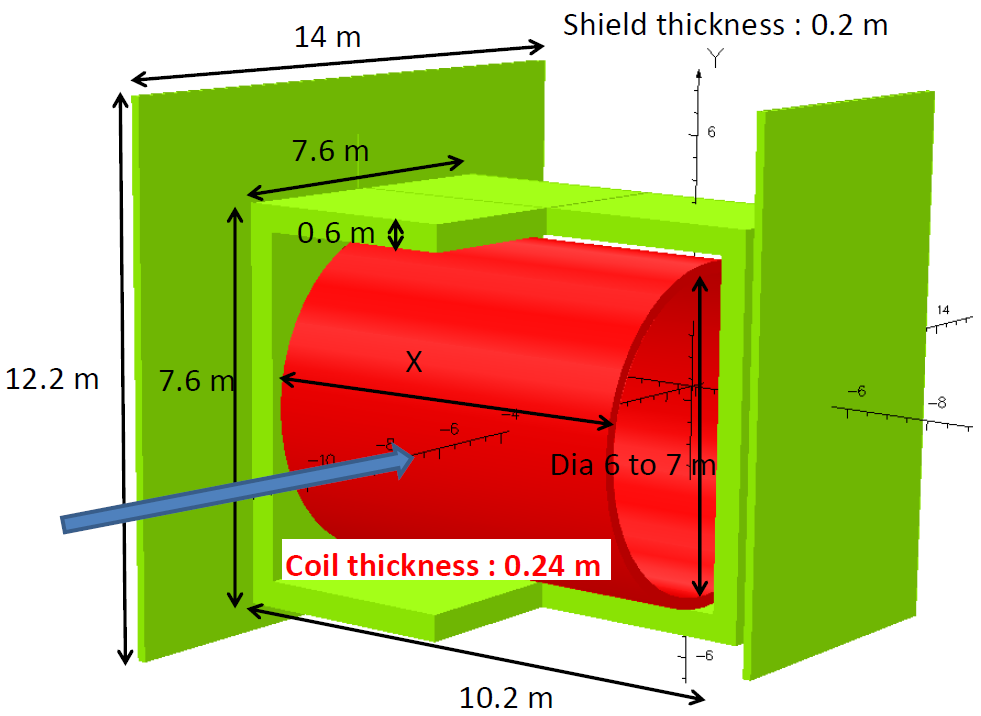
\includegraphics[width=0.95\columnwidth]{graphics/dune_nd_magnet_nc_layout.png} 
\caption{Normal conducting magnet concept} 
\label{fig:dune_nd_magnet_nc_layout} 
\end{figure}
%




\section{Three-Dimensional Projection Scintillator Tracker Spectrometer}
\label{sec:exsum-nd-mpt-3dst}

The three dimensional projection scintillator tracker spectrometer (\dword{3dsts}) consists of an active target core of scintillator called the \dword{3dst} surrounded by \dwords{tpc} and an \dword{ecal} in a 0.4 T magnetic field.  This system has three main goals in the context of the larger \dword{nd} complex.  First, the \dword{3dsts} functions as an on-axis, high mass target and muon spectrometer that is capable of producing a statistically significant neutrino beam spectrum measurement in a short period.  This consistent, on-axis beam monitoring will be important in light of the movement of \dword{arcube} and the \dword{mpd}.  Second, the \dword{3dsts} will provide flux measurements with systematic errors and biases that differ from those in \dword{arcube}.  This will be valuable input in debugging or developing confidence in the overall beam flux model.  Third, the \dword{3dsts} will produce measurements that are potentially useful for improving and increasing the level of confidence in the neutrino interaction model. In particular, the \dword{3dst} can measure neutrons on an event-by-event basis, including those at a lower neutron kinetic energy than those seen by the other components of the \dword{nd}.  


The 3D projection Scintillator Tracker (\dword{3dst}) is a fully active plastic scintillator detector made up of optically isolated 1 cm$^{3}$ cubes \cite{Sgalaberna:2017khy}.  The cubes are read out by wavelength shifting (WLS) fibers along 3 orthogonal axes providing three two-dimensional projections that yield effective three-dimensional reconstruction.  


The \dword{3dst} is dense enough to provide a large statistics sample with reasonable containment of hadrons and photons from neutrino interactions. The high statistics and granularity  of the \dword{3dst} will allow for timely beam monitoring, flux determination via different methods (with charge separation), and the study of many different neutrino interaction morphologies.  The sub-ns timing resolution provides the  capability to include neutrons in the event reconstruction via Time-of-Flight (TOF) with a reasonably high efficiency.  


Neutron production plays a critical role in the interaction model since the near and far \dword{lar} detectors are largely blind to neutrons. Because the neutron content of neutrino and anti-neutrino interactions differ, the model for neutrons is particularly important for a \dwords{cpv} measurement.  Preliminary studies show the \dword{3dst} is likely to be able to measure neutron spectrum to lower neutron KE than other detectors and pursue event-by-event analysis with fully reconstructed final state particles, including neutrons.  GENIE and NuWro event generators both indicate neutron spectra for Ar and C are qualitatively similar.  So, it is plausble that observations of neutrons produced by (anti)neutrino interactions on C can provide a higher level of confidence in the extrapolation of the Ar neutron model to lower KE$_{n}$ than would otherwise be possible.

The \dword{3dst} uses the same technology as the SuperFGD detector that is being constructed for the \dword{t2k} Near Detector upgrade \cite{Abe:2019whr}.  The two detectors are functionally identical, though somewhat different in size.  The SuperFGD will be installed 2021 and will act effectively as a prototype for the larger \dword{3dst} in the \dword{dune}  \dword{nd}. 


\subsection{Detector Configuration}

The \dword{3dst} detector concept is shown in Figure~\ref{fig:cube}.
The scintillator composition is polystyrene doped with 1.5\% of paraterphenyl (PTP) and 0.01\% of POPOP. After fabrication, the scintillator surface of the cubes is etched with a chemical agent that results in the formation of a white, reflecting polystyrene micropore deposit over the scintillator. Three orthogonal through holes of 1.5 mm diameter are drilled in the cubes to accommodate WLS fibers. 
This novel geometry provides full angular coverage for particle produced in neutrino interactions.  The momentum threshold for protons is about 300 MeV/c (if at least three hits are requested).


\begin{figure}
\begin{center}
  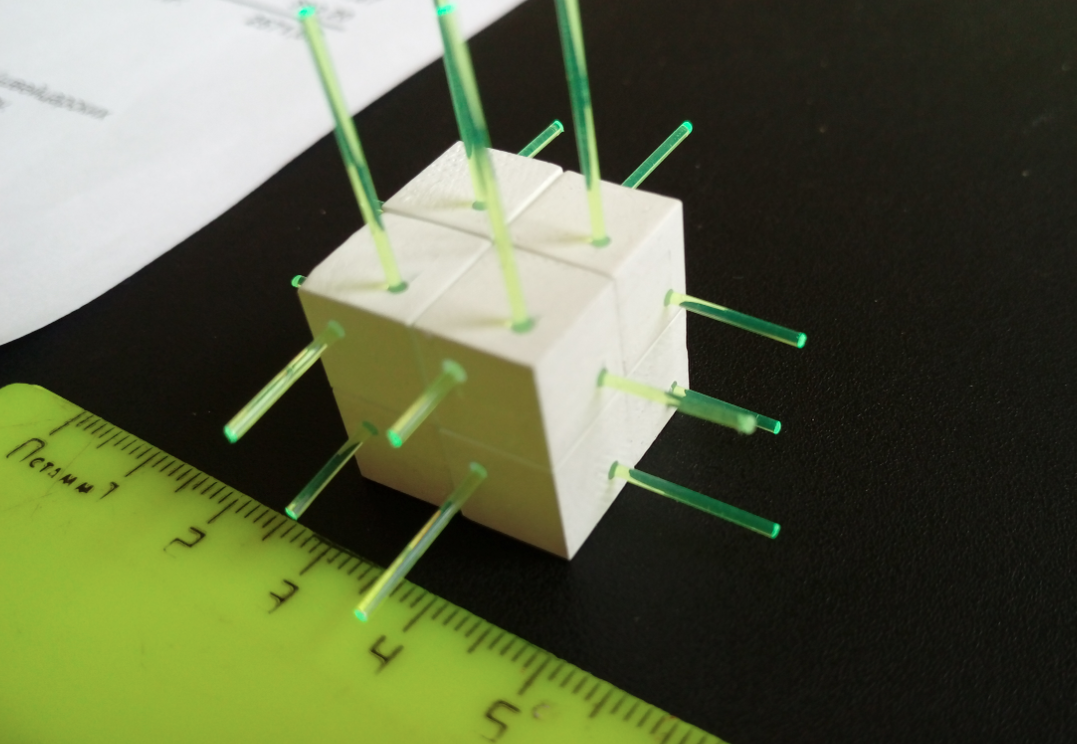
\includegraphics[width=3.in]{cube.png}
\caption{\label{fig:cube}
A few plastic scintillator cubes assembled with WLS fibers are shown.}
\end{center}
\end{figure}

The \dword{3dst} and surrounding elements are shown in Figure~\ref{fig:3dst-geometry}.  The size of the \dword{3dst} detector is under discussion.  Detectors of size 2.4$\times$2.4$\times$2.0~m$^{3}$, 3.0$\times$2.0$\times$2.0~m$^{3}$, and 2.0$\times$2.0$\times$2.0~m$^{3}$ have been used in different studies.  The primary considerations that drive the size are space, statistics, and neutron containment.
The \dword{3dst} is surrounded by \dwords{tpc} to measure the kinematics of charged particles produced but not stopping in \dword{3dst}, and an \dword{ecal} to identify and reconstruct photons and electrons exiting the \dword{3dst}. All the detectors will be immersed in a 0.4~T magnetic field provided by the magnet. The outer dimension of the whole system is approximately 5(width)$\times$5(height)$\times$3(length)~m$^3$. 
%The collective structure of the \dword{3dst} and surrounding detectors and magnet is called the 3 dimensional projection scintillator detector spectrometer, or \dword{3dsts}.


\begin{figure}
\begin{center}
  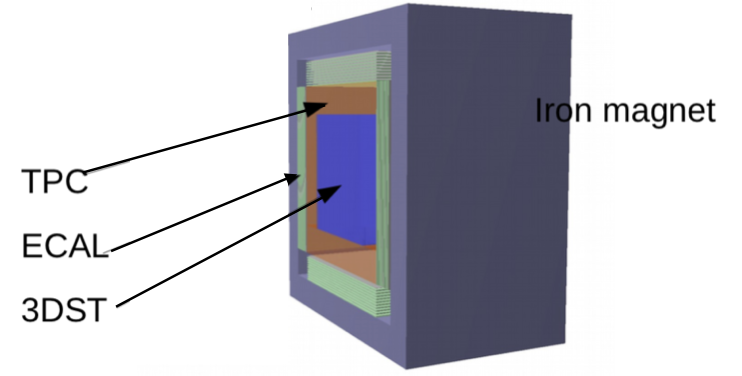
\includegraphics[width=7.in]{3dst-geometry.png}
\caption{\label{fig:3dst-geometry}
The \dword{3dsts} detector configuration, including the \dword{3dst} (blue), \dwords{tpc} (orange), \dword{ecal} (green), and the magnet (purple) is shown.} 
\end{center}
\end{figure}



\subsection{3DST Detector Performance}

The performance of devices built on the \dword{3dst} concept have been tested in several test beams at CERN \cite{Mineev:2018ekk}.
A small prototype of $5\times5\times5$ cubes collected data in the T10 test-beam area at CERN in 2017, with the goal of characterizing the response of the plastic scintillator cubes.
The detector was instrumented with 75 WLS fibers (1 mm diameter Y11(200) Kuraray S-type of 1.3 m length). One end of the fiber was attached to a photosensor while the other end was covered by a reflective Al-based paint (Silvershine). The photosensors in the beam test were Hamamatsu MPPCs 12571-025C with a $1\times1~\text{mm}^2$ active area and 1600 pixels. The data were collected with a 16-channel CAEN digitizer DT5742 with 5 GHz sampling rate and 12-bit resolution.

The average light yield was about 40 p.e./MIP in a single fiber, and the total light yield from two fibers in the same cube was measured on an event-by-event basis to be about 80 p.e., as expected.
The light cross-talk probability between a cube fired by a charged particle and a neighbouring cube was studied. The light measured in the neighbouring cube was about 3.4\% of the light collected from the fired cube. 
The timing resolution for a single fiber was measured to be $\sim$0.95~ns. If the light of a cube is read out by two WLS fibers, the timing resolution becomes better then 0.7~ns and would improve further if the light collected by all the three WLS fibers is taken into account.
In Figure~\ref{fig:testbeam2017} the light yield and the time spectra obtained from two fibers reading out the light in the same cube are shown.

\begin{figure}
\begin{center}
  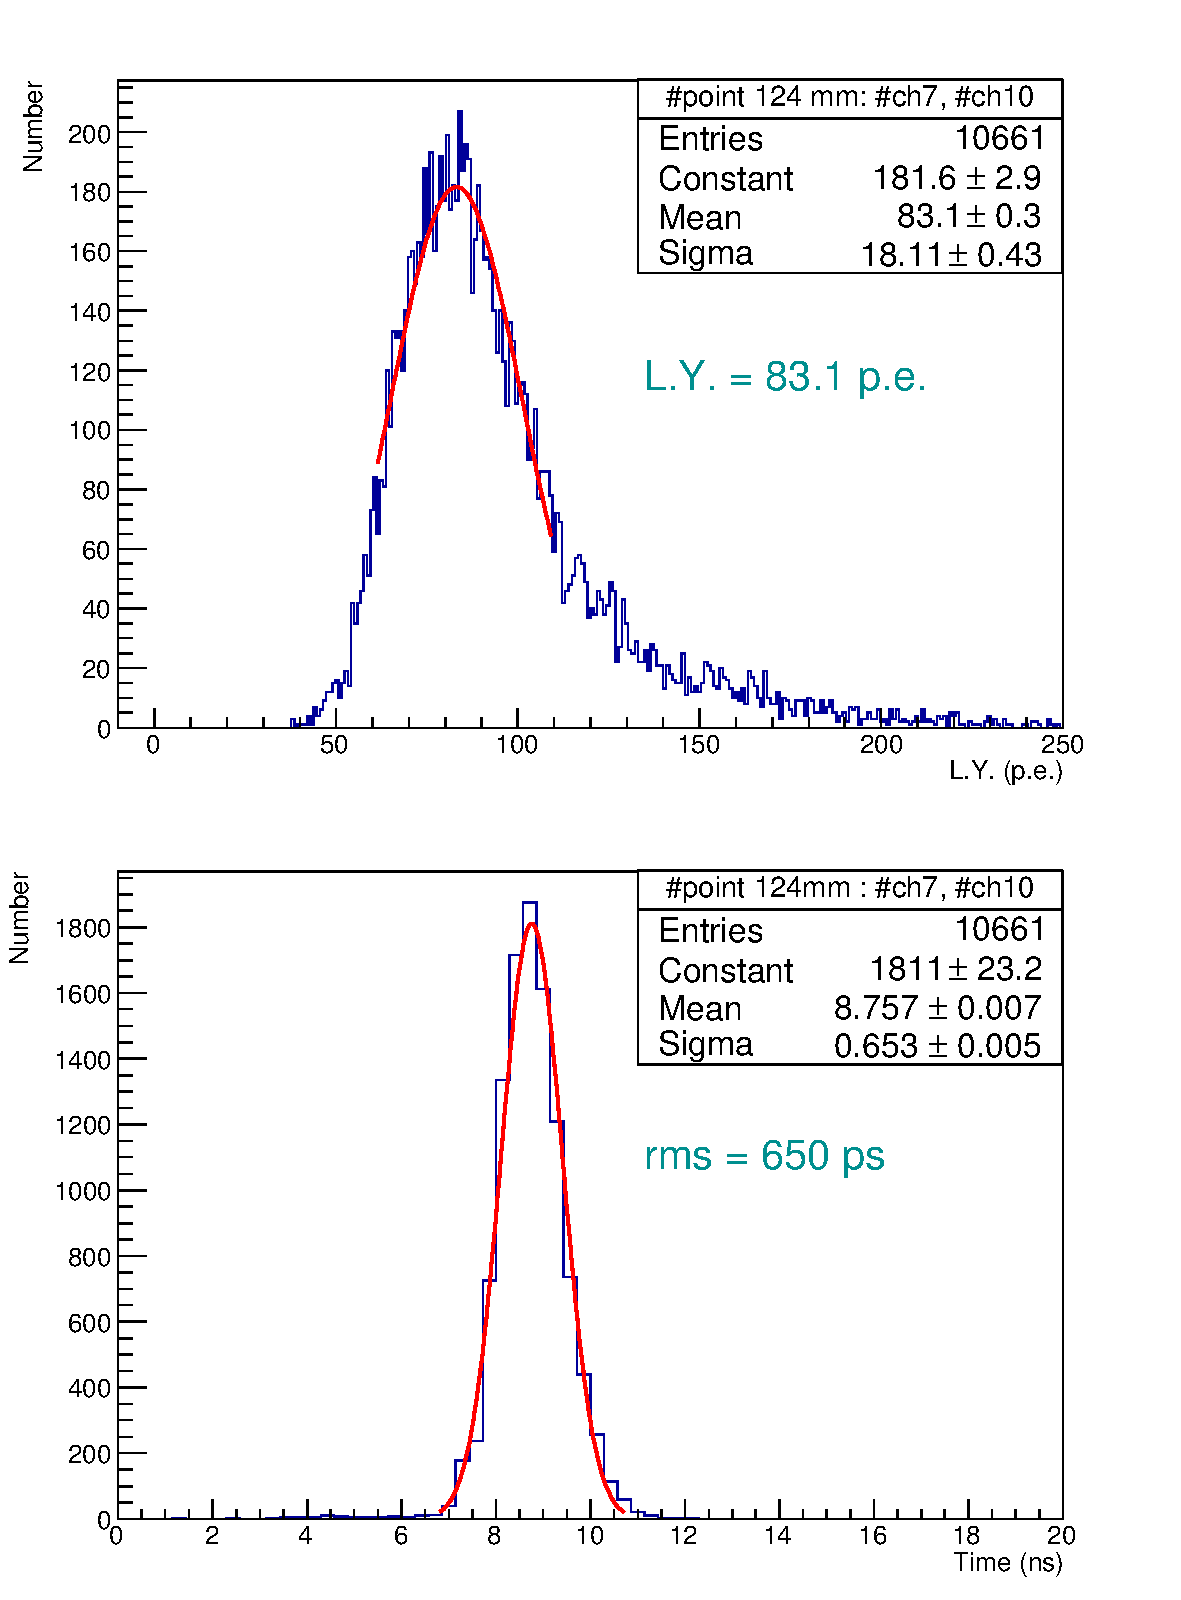
\includegraphics[width=3.5in]{Target_cube_spectra.pdf}
\caption{\label{fig:testbeam2017} Charge and time spectra for a single cube. Charge signal is a sum from two fibers, the time is an average time between two fibers.} 
\end{center}
\end{figure}

In the summer of 2018, a new prototype made of 9,216 cubes with a size of 8$\times$24$\times$48~cm$^{3}$  collected data in the CERN T9 test-beam line.
A different electronic readout was used, which was based on the CITIROC chip used in the Baby MIND experiment.
Preliminary results confirmed the light yield performances of the 2017 test-beam data. A more detailed analysis of the data is currently ongoing.
Some event displays are shown in Figure~\ref{fig:testbeam2018}.

\begin{figure}
\begin{center}
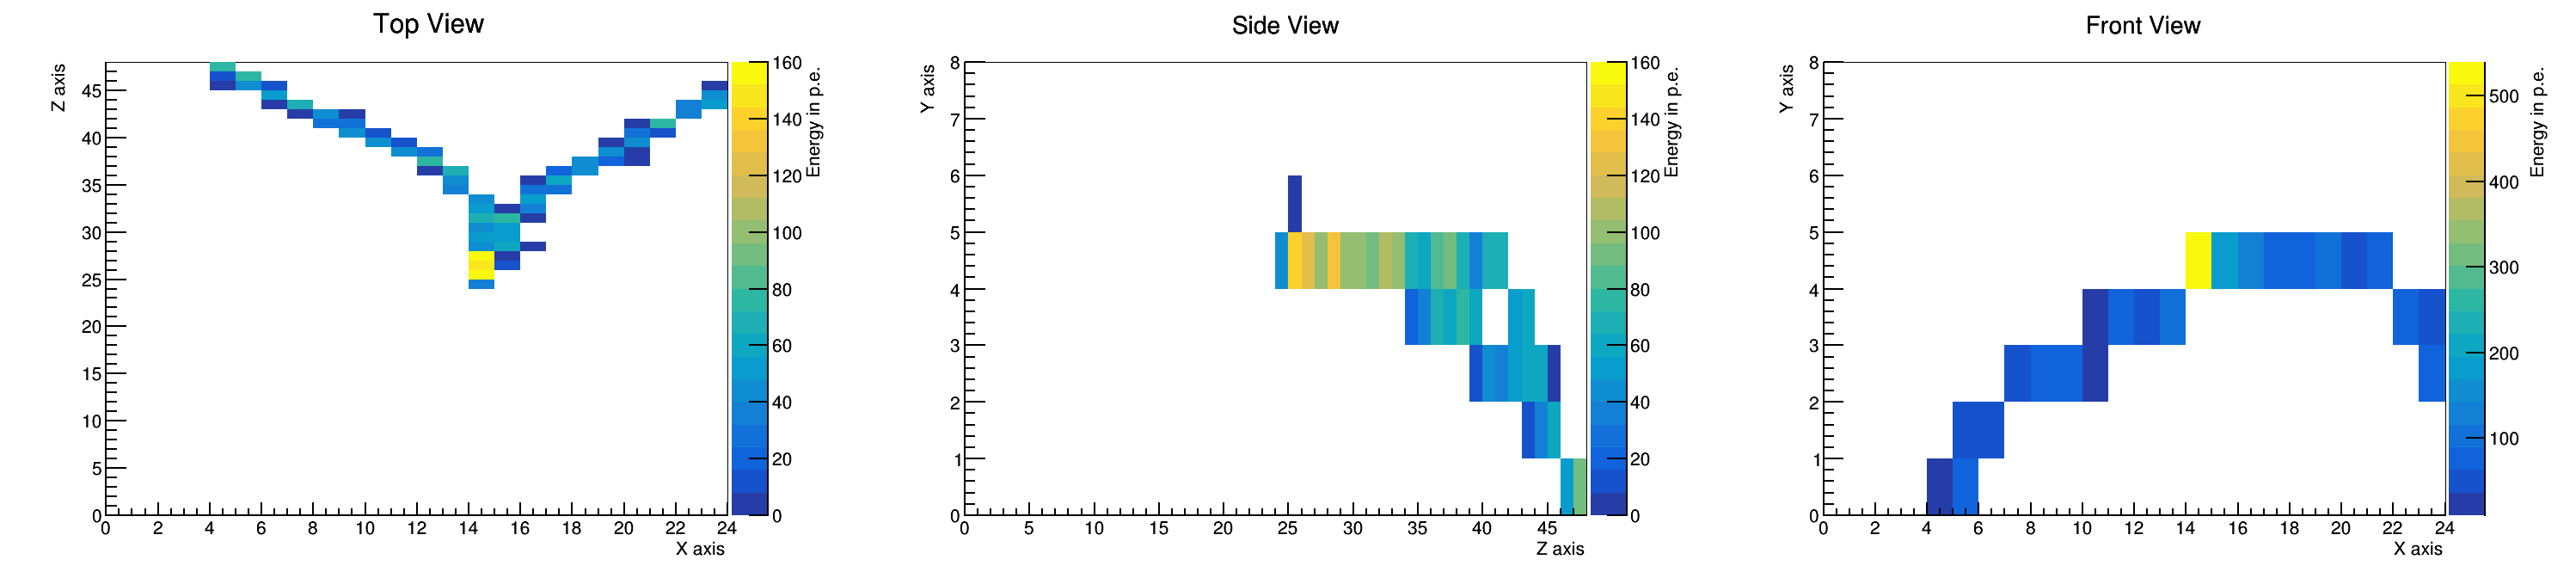
\includegraphics[width=7.5in]{Target_photon_conversion.png}
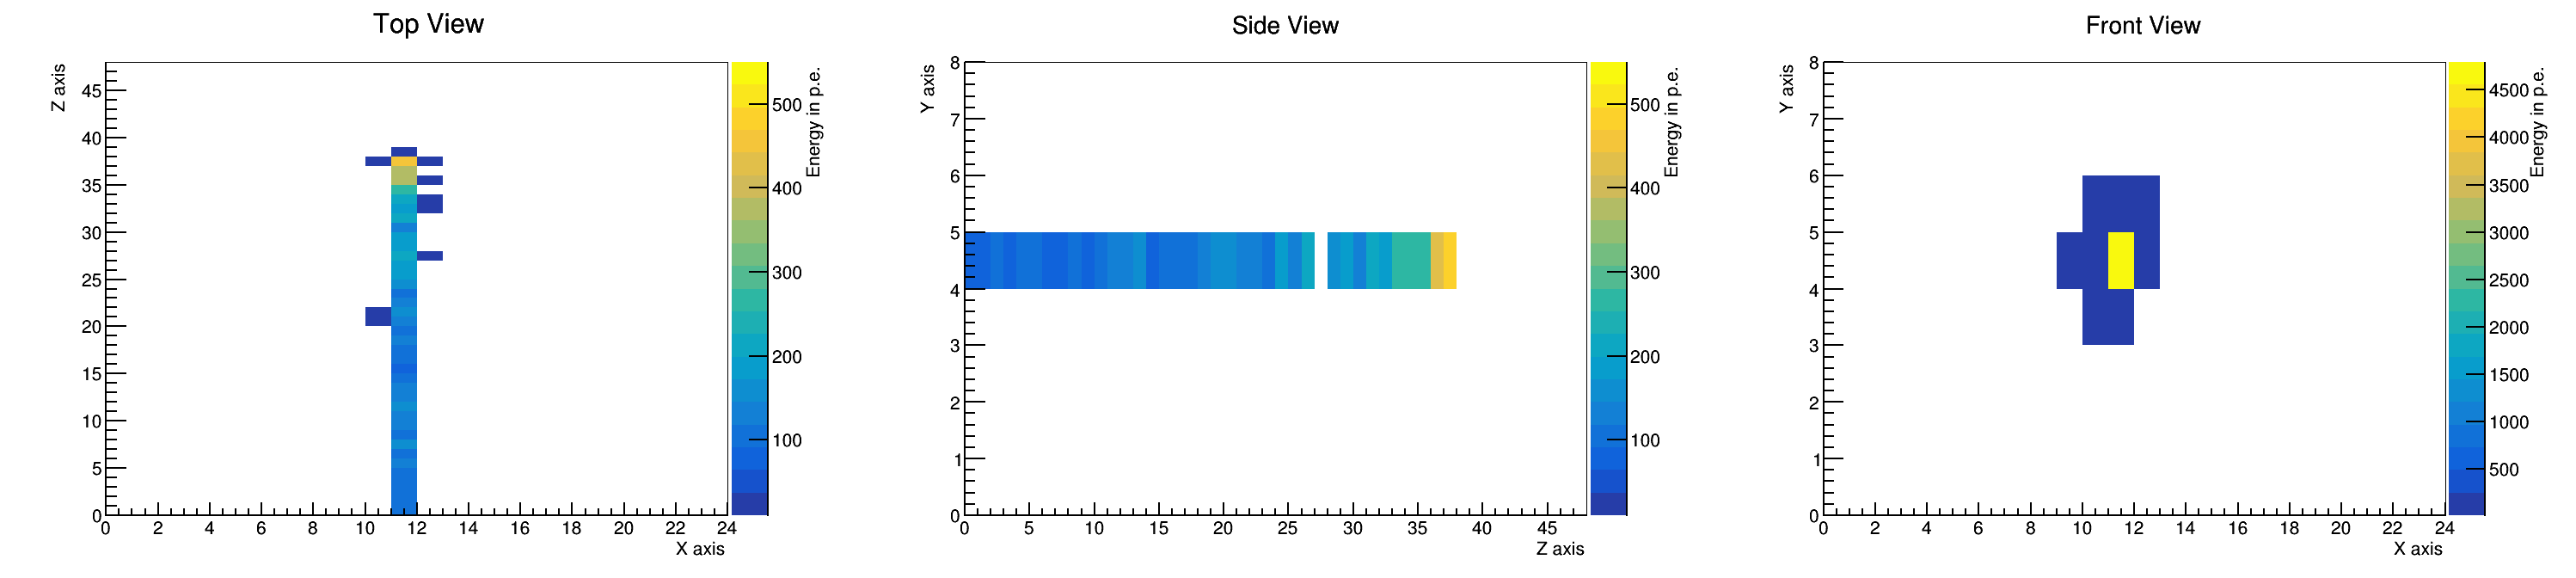
\includegraphics[width=7.5in]{Target_stopped_proton.png}
\caption{\label{fig:testbeam2018} Event displays showing the three two-dimensional projections of energy from a photon conversion (top) and a stopping proton (bottom). From data collected at the 2018 test beams at the CERN T9 area.} 
\end{center}
\end{figure}



\subsection{Neutron Detection Performance}

The \dword{minerva} experiment demonstrated the ability of measuring neutrons produced in neutrino interactions with a plastic scintillator detector~\cite{Elkins:2019vmy}. 
The \dword{3dst} should be able to do this far better than \dword{minerva} because of its high granularity and exquisite timing resolution (both much better than \dword{minerva}). 

Studies indicate that the \dword{3dst} can detect neutrons with a high efficiency and measure their energy via ToF on a particle-by-particle basis.  This is likely to be helpful for 
understanding/improving both neutrino and antineutrino interaction models, and of potential use when faced with "unknown unknown" sources of systematic uncertainties. The argon-based detectors in the \dword{nd} complex are also expected to have some ability to detect neutrons, but studies indicate the sensitivity will be limited to regions of relatively high neutron kinetic energy.  The \dword{3dst} will be sensitive to neutrons down to significantly lower kinetic energy.  Though the measurements are on carbon, generator truth studies show the neutron spectra in neutrino interactions on carbon and argon are qualitatively similar. Thus the measurements at low neutron kinetic energy in the \dword{3dst} can provide additional confidence in the argon neutron model at energies lower than those accessible in the other detectors. 

Neutron scattering can  be seen clearly in \dword{3dst} simulations. 
Figure~\ref{fig:NeutronDisplay} shows an example of
$\overline{\nu}_{\mu}$ \dword{cc}  single charged pion interaction. The neutron-induced energy deposition due to proton recoil can be seen apart from the vertex region. 
Inspired by \dword{minerva}, our recent studies have shown that the \dword{3dst} can tag the presence of neutrons as well as determine the neutron energy via time-of-flight. \\


\begin{figure}
\begin{center}
  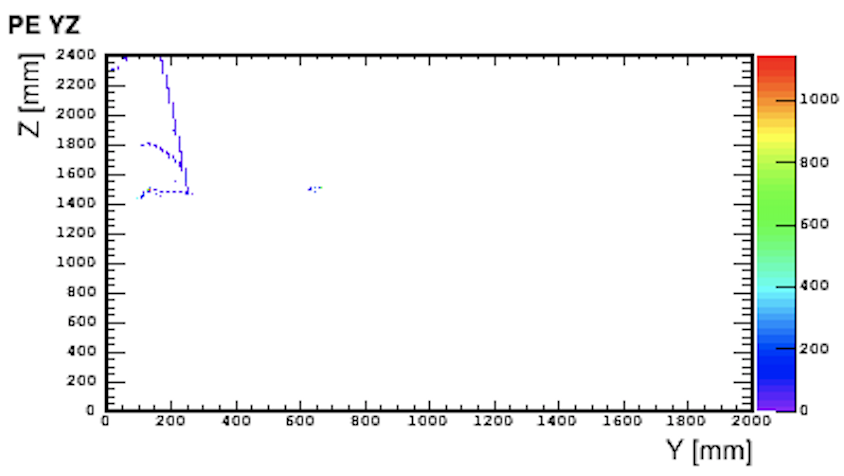
\includegraphics[width=5in]{event-display-neutron-yz.png}
\caption{\label{fig:NeutronDisplay} An example of the antineutrino
%CC1$\pi^{+}$ 
interaction in a 2.4$\times$2.4$\times$2.0~m$^{3}$ \dword{3dst}. 
The number of photo-electrons (PE) is plotted.
An isolated cluster of hits 
corresponds to a neutron indirect signature produced by the antineutrino interaction.
} 
\end{center}
\end{figure}

With a 2.4$\times$2.4$\times$2.0~m$^{3}$ \dword{3dst} detector, Figure~\ref{fig:nProposal_4} shows 
the reconstructed neutron energy residual for 100 MeV kinetic energy neutron using time-of-flight with a lever arm (distance between neutron hit and neutrino vertex) larger than 0.5~m and smaller than 1~m.
This study was conducted with a neutron particle gun simulation.
The tail is due to both the timing resolution as well as the mis-reconstructed neutron flight distance due to non-visible interactions like elastic scattering with Carbon.
The neutron energy resolution is about 18\%. \\
\begin{figure}
\begin{center}
  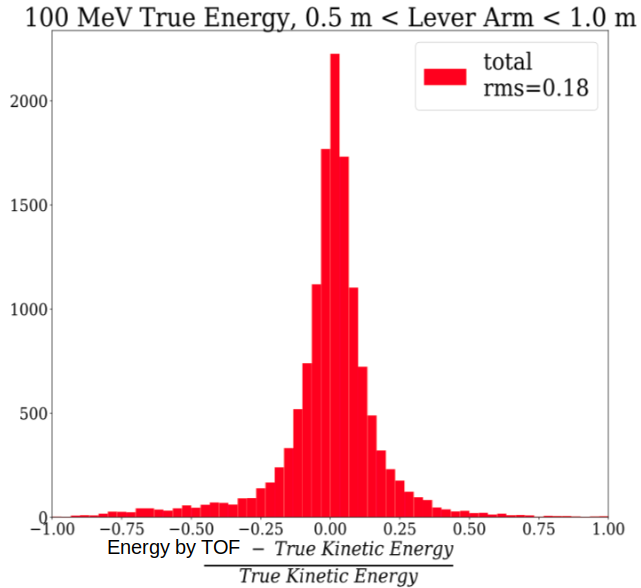
\includegraphics[width=5in]{neutronERes.png}
\caption{\label{fig:nProposal_4} Reconstructed neutron energy residual with lever arm larger than 0.5~m and smaller than 1~m for 100 MeV for a 2.4$\times$2.4$\times$2.0~m$^{3}$ \dword{3dst} detector. } 
\end{center}
\end{figure}

 Neutrons produced by neutrino interactions happening outside the \dword{3dst} fiducial volume (out-FV), such as in the \dword{ecal}, Magnet, front detector, and rock can act as a background to the neutron signal from neutrino interactions. 
A simulation study was performed to understand the significance of background. In this study, the \dword{3dsts} was place in an underground alcove and significant dead material was placed upstream.  The FV was taken to be an inner core of 1.0$\times$1.0$\times$1.0~m$^{3}$ of scintillator inside a \dword{3dst} of size 2.0$\times$2.0$\times$2.0~m$^{3}$.  Neutrino beam spills of separation 1.3~s and a uniform neutrino time distribution within each spill were used.
For each neutrino interaction occurring inside the FV, the 
 the earliest neutron-induced hit leaving an energy greater than 0.5 MeV in one cube was recorded. This threshold is thought to be conservative for the \dword{3dst} system.  If that hit was from the neutrino interaction vertex, it was considered a signal neutron-induced hit. On the other hand, if that hit was created by a particle from out-FV, it was considered a background neutron-induced hit.
Figure~\ref{fig:neutronBG1} shows the time difference between the neutrino interaction vertex time ($t_{vtx}$) and the following earliest neutron-induced hit time ($t_{neutron}$). 
Note that a pure signal neutron sample can be obtained by cutting on ($t_{neutron} - t_{vtx}$). 
\begin{figure}
\begin{center}
  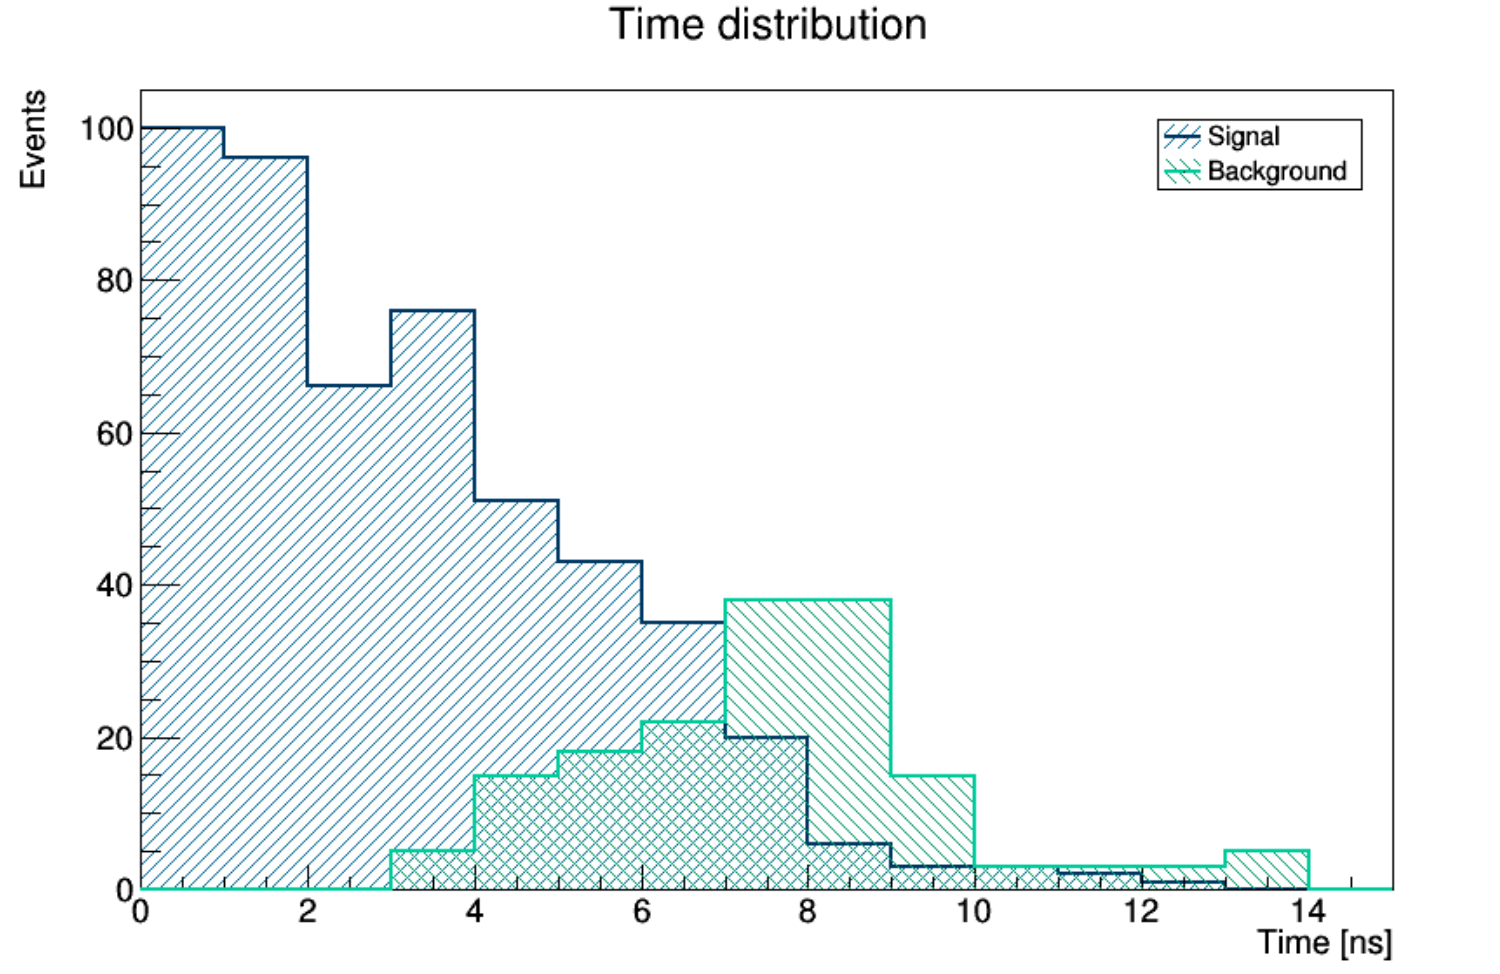
\includegraphics[width=5.2in]{timeDist.png}
\caption{\label{fig:neutronBG1} Time difference between the neutrino interaction vertex time inside the 1.0$\times$1.0$\times$1.0~m$^{3}$ fiducial volume core of the \dword{3dst} and the earliest neutron-induced hit time. The neutron-induced hit leaves at least 0.5 MeV in a single cube. Neutron-induced background hits are considered as all neutrino interactions happening outside FV.
} 
\end{center}
\end{figure}

In this study, a veto was not used on \dword{cc} and NC interactions with pions in the materials surrounding the \dword{3dst}.  Such a veto can be implemented and should reduce the backgrounds substantially.  This will be investigated in the future.

To quantify the background, the purity is defined as the ratio of events where the first neutron-induced hit by time is from the signal vertex to all events which have a neutron-induced hit in the FV. 
Figure~\ref{fig:nominal_purity} shows the purity in time - lever arm space. 
\begin{figure}
\begin{center}
  %\includegraphics[width=5in]{nominal_purity3.png}
  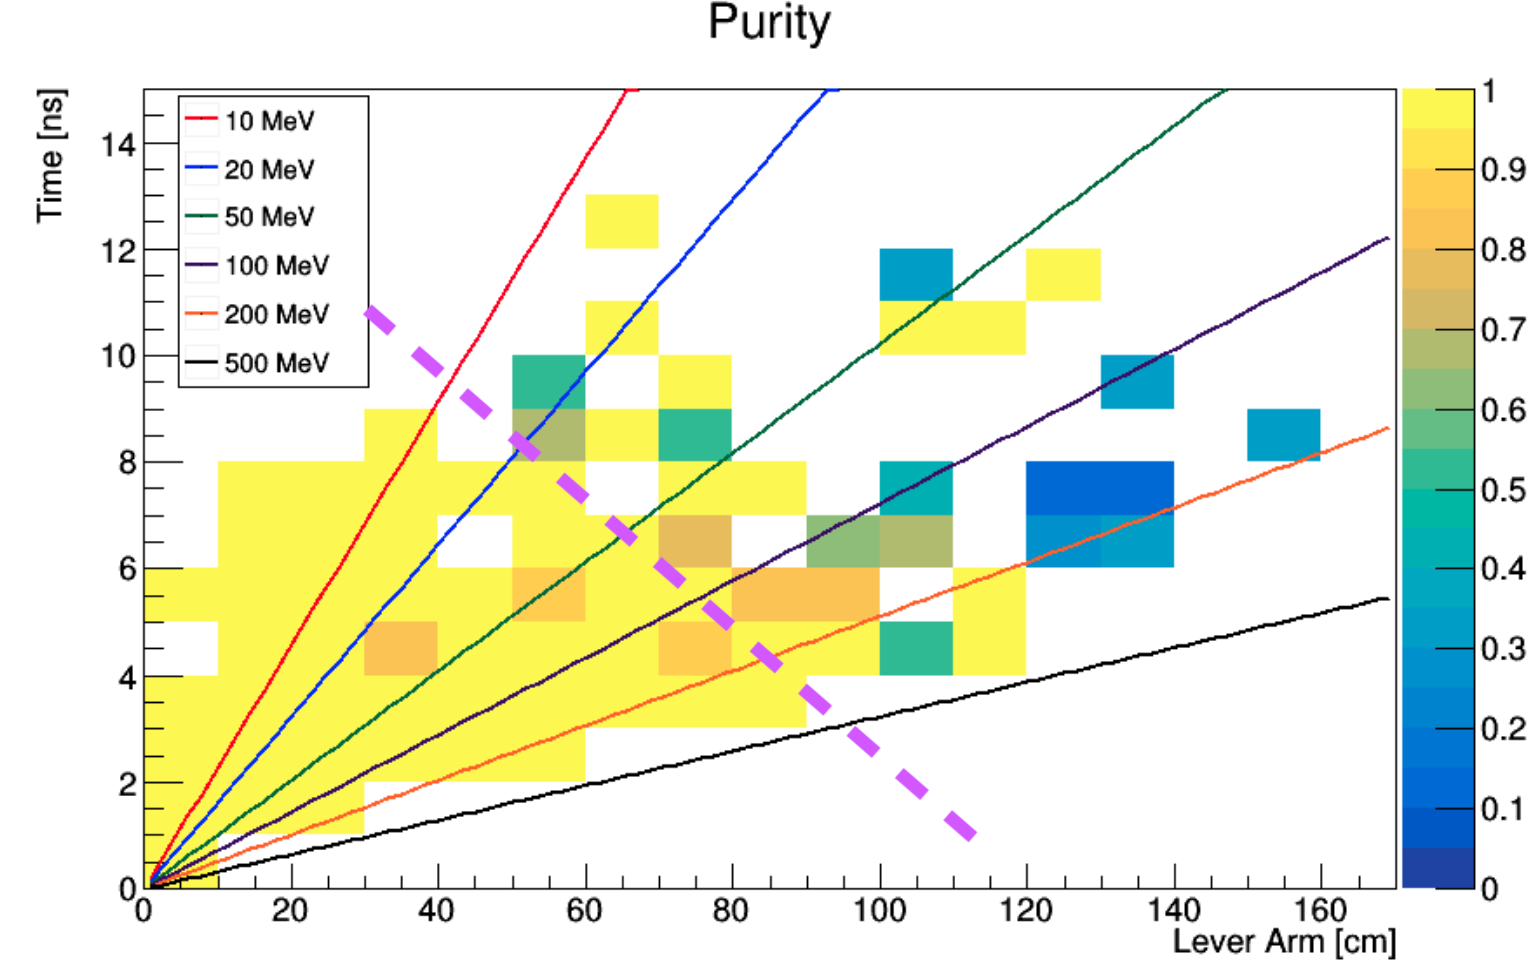
\includegraphics[width=5in]{nominal_purity3-cut.png}
\caption{\label{fig:nominal_purity} Purity of the neutron-induced hit in the (time, lever arm) space.
The dashed line corresponds to the cut required to select an almost 100\% pure sample of signal neutrons. The solid lines are theoretical curves for neutrons with different kinetic energies.
Note that this study was performed with a total volume of 2$\times$2$\times$2 m$^3$.
See text for details.} 
\end{center}
\end{figure}


The reconstructed energy resolution in the same (time, lever arm) 2D space was studied. For this work, the time was smeared by 0.58~ns, corresponding to a per fiber time resolution of 1~ns (the documented performance in the CERN test beam is 0.9~ns).
Though higher light yield can help reduce the time resolution, this effect has not been taken into account. Figure~\ref{fig:nominal_resolution} shows the reconstructed-by-ToF neutron energy resolution. In general, $\sim 20 \%$ energy resolution can be reached with most of the lever arm and time windows, 
in the region selected by the background cut. \\
\begin{figure}
\begin{center}
  %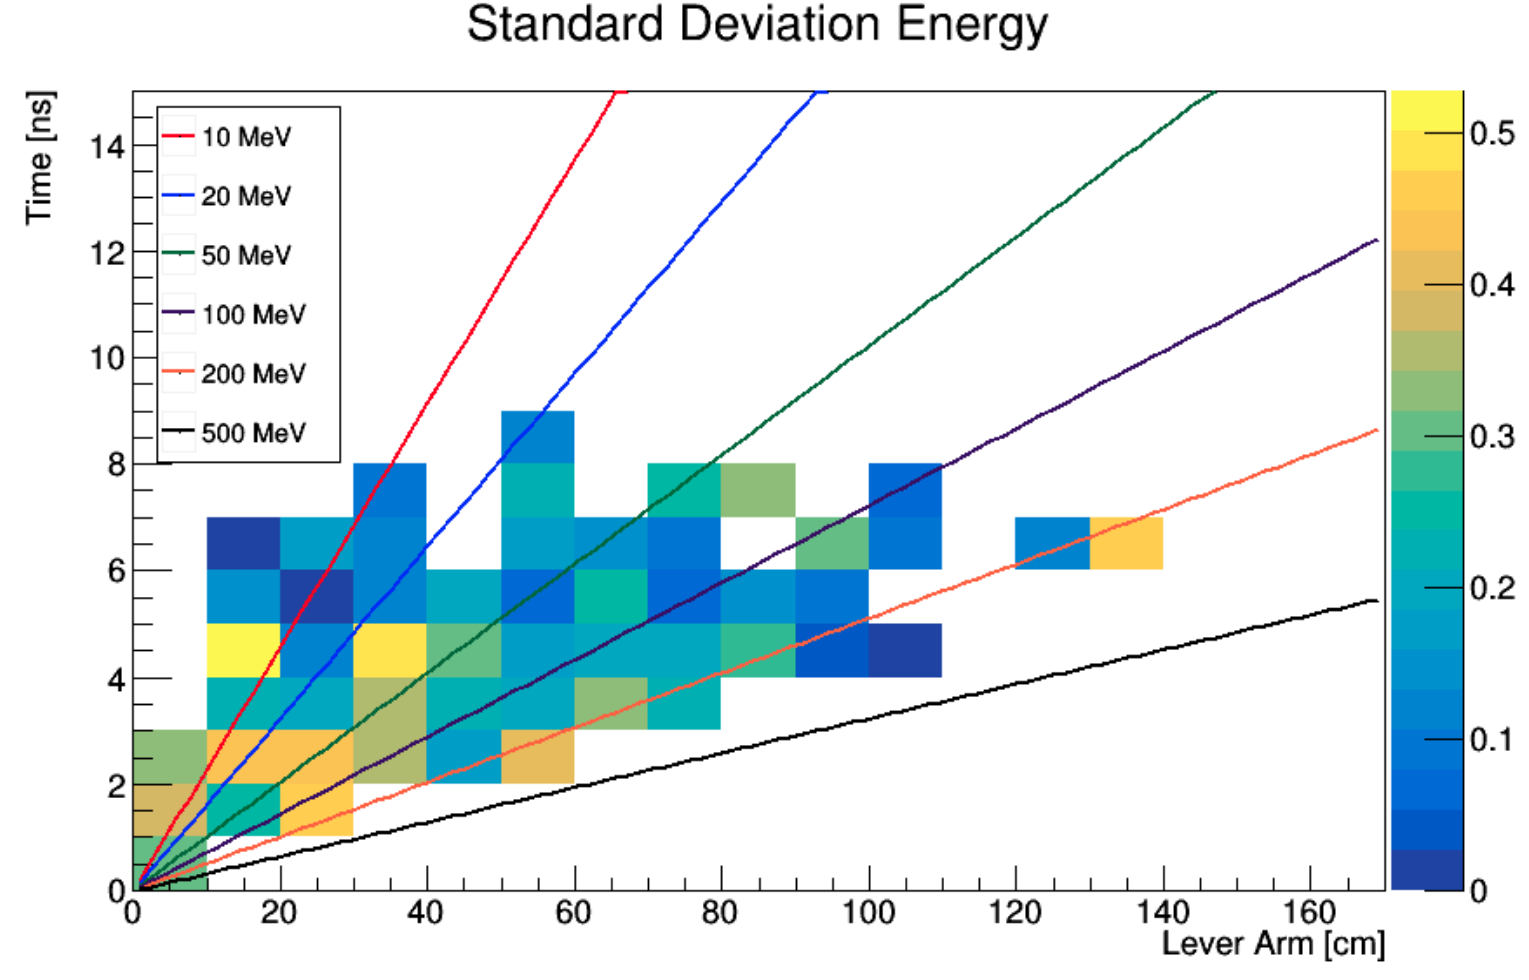
\includegraphics[width=5in]{nominal_resolution3.png}
  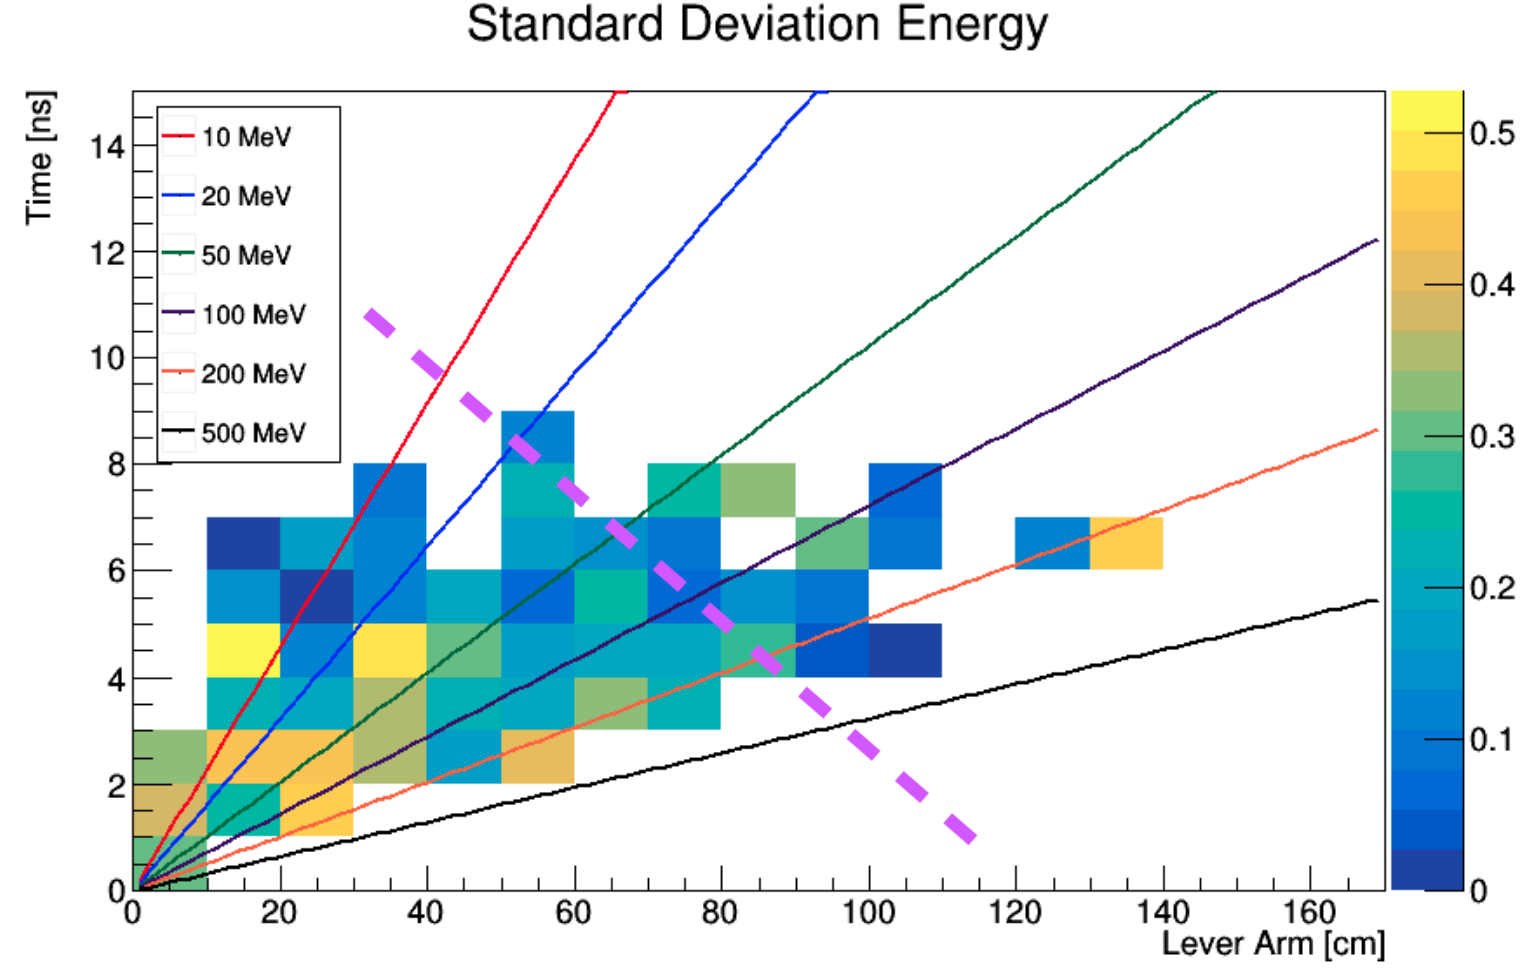
\includegraphics[width=5in]{nominal_resolution3-cut.png}
\caption{\label{fig:nominal_resolution} Energy resolution of the neutron-induced hit in the (time, lever arm) space. 
The dashed line corresponds to the cut required to select an almost 100\% pure sample of signal neutrons. The solid lines are theoretical curves for neutrons with different kinetic energies.
Note that this study was performed with a total volume of 2.0$\times$2.0$\times$2.0~m$^3$.
See text for details.} 
\end{center}
\end{figure}


\subsection{Expected Statistics}


The default size of the \dword{3dst} is defined to be 2.4$\times$2.4$\times$2.0~m$^{3}$. This gives a total target mass for the \dword{3dst} of 12 metric tons.  Implementing a generic veto region around each side of the detector of 10 cm, gives a fiducial mass of 8.7~tons.
Table~\ref{tab:stats} gives the number of events expected per year in the fiducial volume of such a \dword{3dst} detector.  The numbers given in the table are assuming the 80 GeV, 3 horn, optimized LBNF beam flux and 1.46$\times10^{21}$~POT/year.

\begin{table}
\begin{center}
\begin{tabular}{| c | c | c |}
\hline
Channel & $\nu$ mode & $\bar{\nu}$ mode \\
\hline
$\nu_{\mu}$ \dword{cc} inclusive & 13.6$\times$10$^{6}$ & 5.1$\times$10$^{6}$ \\ 
\dword{ccqe} & 2.9$\times$10$^{6}$ & 1.6$\times$10$^{6}$ \\
\dword{cc} $\pi^{\circ}$ inclusive & 3.8$\times$10$^{6}$ & 0.97$\times$10$^{6}$ \\
NC total & 4.9$\times$10$^{6}$ & 2.1$\times$10$^{6}$ \\
$\nu_{\mu}$-e$^{-}$ scattering & 1067 & 1008 \\
$\nu_{e}$ \dword{cc} inclusive & 2.5$\times$10$^{5}$ & 0.56$\times$10$^{5}$ \\
 \hline
\end{tabular}
\end{center}
\caption{\label{tab:stats} This table summarizes the projected event rates per year for a 2.4~x~2.4~x~2.0~m$^{3}$ \dword{3dst} detector, assuming the 80 GeV, three horn, optimized LBNF beam. A 10~cm veto region at each side was required. }
\end{table}




\subsection{Beam Monitoring}

In the context of \dword{duneprism}, the \dword{lartpc} and \dword{mpd} will move off-axis much of the time. The only detector that could provide a reliable measure of the neutrino spectrum on axis on a daily basis in the  \dword{nd} hall is the \dword{3dst}. History shows such monitoring is necessary. 




%%%%%%%%%%%%%%%%%%%%%%%%%%%%%%%%%%%%%%%%%%%%%%%%%%%%%%%%%%%%%%
\section{DUNE-PRISM}
\label{sec:exsum-nd-DP}


One of the primary challenges for \dword{dune} will be controlling systematic uncertainties from the modeling of neutrino-argon interactions. The relationship between the observable final state particles from a neutrino interaction and the incident neutrino energy is currently not understood with sufficient precision to achieve \dword{dune} physics goals due to missing energy from undetected particles, such a neutrons and low energy charged pions, and misidentified particles. These effects tend to cause  a ``feed-down" in reconstructed neutrino energy relative to the true energy. Since neutrino energy spectra at the far and \dwords{nd} have substantially different features due to the presence of oscillations at the  \dword{fd}, these neutrino energy feed-down effects do not cancel in a far/near ratio as a function of neutrino energy, and lead to biases in the measured oscillation parameters.

Understanding  \dword{nd} constraints on neutrino-nucleus interaction uncertainties is challenging, since no complete model of neutrino-argon interactions is available. If it were possible to construct a model that was known to be correct, even with a large number of unknown parameters, then the task of a  \dword{nd} would much simpler: to build a detector that can constrain the unknown parameters of the model. However, in the absence of such a model, this procedure will be subject to unknown biases due to the interaction model itself, which are difficult to quantify or constrain.

The \dword{duneprism}  \dword{nd} program consists of a mobile  \dword{nd} that can perform measurements over a range of angles off-axis from the neutrino beam direction in order to sample many different neutrino energy distributions, as shown in Figure~\ref{fig:offaxisfluxes}. By measuring the neutrino-interaction final state observables over these continuously varying incident neutrino energy spectra, it is possible to experimentally determine the relationship between neutrino energy and what is measured in the detector.

\begin{figure}[h!]
   \begin{center}
      \includegraphics[width=0.65\textwidth]{offaxisfluxes.pdf}
      \caption{The variation in the neutrino energy spectrum is shown as a function of detector off-axis position, assuming the nominal near detector location 574~m downstream from the production target.}
      \label{fig:offaxisfluxes}
   \end{center}
\end{figure}


The goals of the off-axis measurements are twofold:
\begin{itemize}
\item {\bf To identify problems in the cross section modeling.} By comparing  \dword{nd} data to MC at many off-axis locations with different energy spectra, the neutrino interaction model will be over-constrained, and the potential for biases in the measured oscillation parameters can be identified.
\item {\bf To overcome problems in the cross section modeling.} The most important novel feature of a \dword{duneprism} detector is that measurements at different off-axis positions can be linearly combined to determine any set of observables for any user-defined neutrino energy spectrum. In particular, it is possible to produce oscillated energy spectra using linear combinations of  \dword{nd} off-axis spectra, which would reduce the dependence on neutrino interaction modeling within the oscillation analysis.
\end{itemize}

\subsection{Impact of Cross Section Modeling on Neutrino Oscillations}

One strategy to understand the potential impact of using imperfect neutrino interaction models to measure oscillation parameters is to produce fake datasets that include modifications to the neutrino interaction cross sections that are unknown to the model being used to fit the fake data. In this way, it is possible to understand potential biases in the measured oscillation parameter values extracted from a full near+far detector fit due to the use of an incorrect cross section model in the fit. 

The fake data set considered here assumes that 20\% of the kinetic energy that the interaction model originally assigned to protons was instead carried away by neutrons. The resulting model is then further modified by adjusting the differential cross section in proton energy as a function of true neutrino energy until the measured kinematic distributions in the on-axis  \dword{nd} match the prediction from the default model. This procedure is similar to actions that are routinely taken in actual neutrino oscillation experiments to resolved discrepancies between  \dword{nd} data and the Monte Carlo simulation. There are many potential modifications to the cross section model that can be chosen to resolve such disagreements, and incorrect choices can lead to biased oscillation parameter measurements.



The resulting fake data is analyzed as though it were the actual data taken by the experiment. The near and  \dword{fd} data are simultaneously fit to constrain nuisance parameters in the flux and cross section models, and to extract the measured value of the neutrino oscillation parameters. The results of this fit are shown in Figure~\ref{fig:duneprismfit}. The fit to the fake data shows a clear bias in the measured oscillation parameter values that outside the 95\% confidence limit contours.

\begin{figure}[h!]
   \begin{center}
      \includegraphics[width=0.85\textwidth]{fakedatafitresults.png}
      \caption{The results of a full 4-flavor near+far oscillation fit are shown for a fit to the nominal MC (dashed) and a fit to the fake dataset (solid). The true values of the oscillation parameters in each of the datasets are indicated by the dashed yellow lines. Clear biases can be see in all oscillation parameters that are well outside the 1$\sigma$ (black), 2$\sigma$ (red), and 3$\sigma$ (blue) contours.}
      \label{fig:duneprismfit}
   \end{center}
\end{figure}

A comparison of the fake data and the nominal Monte Carlo reconstruction energy distributions is shown in Figure~\ref{fig:duneprismerec}. In the on-axis location, good agreement is seen, as was intended in the construction of the fake data samples. Conversely, clear disagreement is seen between these sample when moving off-axis. As the off-axis location is varied, this comparison can be made across a wide range of neutrino energy distributions.

\begin{figure}[h!]
   \begin{center}
      \includegraphics[width=0.45\textwidth]{onaxiserec.png}
      \includegraphics[width=0.45\textwidth]{offaxiserec.png}
      \caption{A comparison between the fake data (green) and nominal Monte Carlo (red) reconstructed neutrino energy distributions are shown for the on-axis  \dword{nd} location (left) and a position 18~m off-axis (right).}
      \label{fig:duneprismerec}
   \end{center}
\end{figure}

\subsection{DUNE-PRISM Linear Combination Analysis}

In addition to identifying problems in cross section modeling, \dword{duneprism} measurements provide a mechanism for creating  \dword{fd} predictions directly from the  \dword{nd} data that is largely independent of neutrino interaction modeling. By constructing linear combinations of measurements taken under exposure to different neutrino fluxes, it is possible to determine the distribution of any observable (e.g. reconstructed neutrino energy) for a different neutrino flux of interest. In this way, the  \dword{nd} of an oscillation experiment can be effectively exposed to the same oscillated neutrino flux as the  \dword{fd}, which allows for a direct comparison of any measured observable at the near and  \dword{fd}. This results in a de-coupling of the flux and neutrino interaction uncertainties that otherwise are difficult to disentangle when using a more traditional approach in which the  \dword{nd} is exposed to only a single, unoscillated neutrino flux.



A few example fits of the off-axis near-detector muon neutrino spectra to an oscillated  \dword{fd} muon neutrino energy spectrum are shown in Figure~\ref{fig:duneprismfluxfits}. Good agreement is seen near the first and second oscillation maxima at 2.5~GeV and 0.7~GeV, respectively. This technique can also be applied to match the off-axis muon neutrino spectra to the  \dword{nd} intrinsic electron neutrino spectrum, in order to make a precise measurement of $\sigma(\nu_e)/\sigma(\nu_\mu)$ with a common flux, or to the  \dword{fd} oscillation electron neutrino energy spectra for the measurement of $\delta_{CP}$.

\begin{figure}
	\centering
	\includegraphics[width=0.49\textwidth]{nuprism_coef_oscSpectrum_0_0022_0_5.pdf}
	\includegraphics[width=0.49\textwidth]{nuprism_coef_oscSpectrum_0_0025_0_65.pdf}
\caption{Linear combinations of off-axis fluxes giving far-detector oscillated spectra for a range of oscillation parameters. The  \dword{fd} oscillated flux is shown in black, the target flux is shown in green, and the linearly combined flux obtained with the nominal beam MC is shown in red. Systematic effects due to 1 $\sigma$ variations of the decay pipe radius (green), horn current (magenta) and horn cooling water layer thickness (teal) are shown.}
	\label{fig:duneprismfluxfits}
\end{figure}




%%%%%%%%%%%%%%%%%%%%%%%%%%%%%%%%%%%%%%%%%%%%%%%%%%%%%%%%%%%%%%
\section{ND Hall and Construction}
\label{sec:exsum-nd-hall}
%% \chapter defined in lbne-sci-opp-main.tex

The DUNE near neutrino detector provides scientific value beyond
      its essential role of calibrating beam and neutrino interaction
      properties for the long-baseline physics program described in
      Chapter~\ref{nu-oscil-chap}.
      By virtue of the theoretically clean, purely weak leptonic
      processes involved,
      neutrino beams have historically served as unique probes for
      new physics in their interactions with matter.
      The high intensity and broad energy range of the LBNF beam
      will open the door for a highly capable near detector
      to perform its own diverse
program of incisive investigations. 

%\fixme{Simplified this pgraph a bit per Jim's wish to make the ND seem less optional}
The reduction of systematic uncertainties for the neutrino oscillation
program %of the full DUNE scope requires a highly capable near neutrino detector (ND) to provide 
requires excellent resolution in the
reconstruction of neutrino events. Combined with the unprecedented
neutrino fluxes available %for the DUNE program 
--- which will
allow the collection of ${\cal{O}}$(\num{e8}) inclusive neutrino charged
current (CC) interactions for %\SI{e22}{\POT} 
\num{e22} protons-on-target (POT) just downstream of the
beamline --- the %inclusion of a 
near detector (ND)  %offers a unique opportunity to 
will significantly enhance the DUNE long-baseline 
oscillation program and produce a range of short-baseline neutrino
scattering physics measurements.  The combined statistics and
resolution expected in the ND will allow precise tests of fundamental
interactions resulting in a better understanding of the structure of
matter. 
Table~\ref{tab:rates} lists the expected number of %muon neutrino
beam-neutrino interactions per ton of detector at the DUNE ND site,
located \SI{459}{\meter} downstream from
the %beginning of the decay pipe
target.  
% \fixme{check this sentence; and the table 7.1 caption says
% 'interactions in the beams' (which is weird) and is for a water
% detector. Is this what you want?}  MB: interactions in the neutrino
% beam are interactions in the near detector when the neutrino beam is
% shining on it.  the calculations were made for water. leave as is
This chapter presents a short description of some of the studies that
can be performed with DUNE's fine-grained near neutrino detector
and gives a flavor of the outstanding physics potential. A more
detailed and complete discussion of the ND physics
potential can be found in~\cite{docdb-6704}.
Appendix~\ref{app-dis} describes neutrino scattering 
kinematics and includes
definitions of the kinematic variables used in this chapter.
\begin{table}[!htb]
\centering
\caption[Interaction rates, $\nu$ mode, per ton
for \SI{1e20}{\POT}, \SI{459}{\meter}, \SI{120}{\GeV}]{Estimated interaction rates in the neutrino (second column) and antineutrino (third column) beams per ton of detector (water) 
  for \SI{1e20}{\POT} at \SI{459}{\meter} assuming neutrino
  cross-section predictions from NUANCE~\cite{Casper:2002sd} and a \GeVadj{120}
  proton beam using the CDR reference design.  Processes are defined at the initial neutrino
  interaction vertex and thus do not include final-state effects. These estimates do not
  include detector efficiencies or acceptance~\cite{DOCDB740,DOCDB783}. 
}
\label{tab:rates}
\begin{tabular}[!htbp]{$L^r^r}%rl}  %$
\toprule
\rowtitlestyle
Production mode & $\nu_\mu$ Events & $\overline\nu_\mu$ Events\\
\toprowrule
CC QE ($\nu_\mu n \rightarrow \mu^- p$)                             & 50,100 & 26,300 \\ \colhline
NC elastic ($\nu_\mu N \rightarrow \nu_\mu N$)                      & 18,800 & 8,980 \\ \colhline
CC resonant $\pi^+$ ($\nu_\mu N \rightarrow \mu^- N \pi^+$)         & 67,800 & 0 \\ \colhline
CC resonant $\pi^-$ ($\overline{\nu}_\mu N \rightarrow \mu^+ N \pi^-$)   & 0      & 20,760 \\ \colhline
CC resonant $\pi^0$ ($\nu_\mu n \rightarrow \mu^- \ p \, \pi^0$)    & 16,200 & 6,700 \\ \colhline
NC resonant $\pi^0$ ($\nu_\mu N \rightarrow \nu_\mu \, N \, \pi^0$) & 16,300 & 7,130 \\ \colhline
NC resonant $\pi^+$ ($\nu_\mu p \rightarrow \nu_\mu \, n \, \pi^+$) & 6,930  & 3,200 \\ \colhline
NC resonant $\pi^-$ ($\nu_\mu n \rightarrow \nu_\mu \, p \, \pi^-$) & 5,980  & 2,570 \\ \colhline
CC DIS ($\nu_\mu N \rightarrow \mu^- X$ or 
$\overline{\nu}_\mu N \rightarrow \mu^+ X$, $W>2$)                     & 66,800 & 13,470 \\ \colhline
NC DIS ($\nu_\mu N \rightarrow \nu_\mu X$ or 
$\overline{\nu}_\mu N \rightarrow \overline{\nu}_\mu X$, $W>2$)                   & 24,100 & 5,560 \\ \colhline
NC coherent $\pi^0$ ($\nu_\mu A \rightarrow \nu_\mu A \pi^0$ or 
$\overline{\nu}_\mu A \rightarrow \overline{\nu}_\mu A \pi^0$
)       & 2,040  & 1,530 \\
CC coherent $\pi^+$ ($\nu_\mu A \rightarrow \mu^- A \pi^+$)         & 3,920  &  0 \\ \colhline
CC coherent $\pi^-$ ($\overline{\nu}_\mu A \rightarrow \mu^+ A \pi^-$)   & 0      & 2,900 \\ \colhline
NC resonant radiative decay ($N^* \rightarrow N \gamma $)          & 110    & 50 \\ \colhline
%Cabbibo-suppressed QE hyperon production & & \\ \colhline
%($\mu^+ \Lambda, \mu^+ \Sigma^0, \mu^+ \Sigma^-$) & 0 & xxx  \\ \colhline
NC elastic electron ($\nu_\mu e^- \rightarrow \nu_\mu e^-$  
or  $\overline{\nu}_\mu e^- \rightarrow \overline{\nu_\mu} e^-$)              & 30  & 17 \\ \colhline
Inverse Muon Decay ($\nu_\mu e \rightarrow \mu^- \nu_e$)            & 12  & 0\\ \colhline
Other                                                              & 42,600 & 15,800 \\ 
\toprule
\rowtitlestyle
Total CC  (rounded)                                                       & 236,000 & 81,000 \\ %81,340 \\
\rowtitlestyle
Total NC+CC  (rounded)                                                      & 322,000 & 115,000 \\%114,980 \\ 
\bottomrule
\end{tabular}
\end{table}
%%%%%%%%%%%%%%%%%%%%%%%%%%%%%%%%%%%%%%%%%%%%%%%%%%%%%%%%%%%%%%%%%%%%
\section{Precision Measurements with Long-Baseline Oscillations}
\label{sec-fluxosc}
From the studies of uncertainties and the impact of the spectral shape
presented in Section~\ref{sec:systs}, it is evident that to fully
realize the goals of the full DUNE scientific program --- in
particular, sensitivity to CP violation and the precision measurement
of the three-flavor oscillation parameters --- it is necessary to
characterize the expected unoscillated neutrino flux with high
precision. In addition to the precise determination of the neutrino
flux, shape and flavor composition, the characterization of different
neutrino interactions and interaction cross sections on a liquid argon target
is necessary to estimate physics backgrounds to the oscillation
measurements.  The high-resolution near tracking detector %such as that
described in Section~\ref{sec:ndproj} can measure the unoscillated flux
normalization, shape and flavor to a few percent using systematically
independent techniques that are %listed here and 
discussed in the following sections.
%%%%%%%%%%%%%%%%%%%%%%%%%%%%%%%%%%%%%%
\subsection{Determination of the Relative Neutrino and Antineutrino Flux} 
\label{sec-lownu0}
The most promising method of determining the shape of the \numu and
\anumu flux is by measuring CC events with low 
hadronic-energy deposition (low-$\nu$) where $\nu$ is the total energy of the
hadrons that are produced after a neutrino interaction, $E_\nu -
E_\mu$. It is important to note that not all the hadrons escape the
remnant nucleus, and intranuclear effects will smear the visible energy
of the hadronic system.  A method of relative flux determination known
as low-$\nu_0$ --- where $\nu_0$ is a given value of visible hadronic
energy in the interaction that is selected to minimize the fraction of
the total interaction energy carried by the hadronic system
--- is well developed~\cite{srmishra-reviewtalk}.  The method follows
from the general expression of the $\nu$-nucleon differential cross
section:
\begin{equation}
{\cal N} (\nu < \nu_0) \simeq C \Phi(E_\nu) \nu_0 \left[ {\cal A} +
\left( \frac{\nu_0}{E_\nu} \right) {\cal B} + \left( \frac{\nu_0}{E_\nu} \right)^2 {\cal C} +
{\cal O} \left( \frac{\nu_0}{E_\nu} \right)^3 \right],
\end{equation}
\noindent
where the coefficients are ${\cal A} = {\cal F}_2$, ${\cal B} = ({\cal
  F}_2 \pm {\cal F}_3)/2$, ${\cal C} = ({\cal F}_2 \mp {\cal F}_3)/6$, 
and ${\cal F}_i =\int^1_0 \int^{\nu_0}_0 F_i(x) dx d\nu$ is the
integral of structure function $F_i(x)$.  
%
The dynamics of
neutrino-nucleon scattering  implies that the number of events in a
given energy bin with hadronic energy $E_{\rm had} < \nu_0$ is
proportional to the (anti)neutrino flux in that energy bin up
to corrections ${\cal O}(\nu_0/E_\nu)$ and ${\cal O}(\nu_0/E_\nu)^2$.
%
The number ${\cal
  N}(\nu<\nu_0)$ is therefore proportional to the flux up to correction factors
of the order ${\cal O} (\nu_0/E_\nu)$ or smaller, which are not
significant for small values of $\nu_0$ at energies $\geq \nu_0$. 
 The coefficients ${\cal A}$, ${\cal B}$ and ${\cal C}$ are
determined for each energy bin and neutrino flavor within the ND data.
DUNE's primary interest is the relative flux
determination, i.e., the neutrino flux in one energy bin relative to that in
another; variations in the coefficients do not affect the
relative flux. The prescription for the relative flux determination is
simple: count the number of %$\nu$ 
neutrino CC events below a certain small
value of hadronic energy ($\nu_0$).  The observed number of events, up
to the correction of the order ${\cal O} (\nu_0/E_\nu)$ due to the
finite $\nu_0$ in each total visible energy bin, is proportional to
the relative flux. The smaller the factor $\nu_0/E_\nu$ is, the smaller
is the correction.  Furthermore, the energy of events passing the
low-$\nu_0$ cut is dominated by the corresponding lepton energy. 
It is
apparent from the above discussion that this method of relative flux
determination is not very sensitive to nucleon structure, QCD
corrections or types of neutrino interactions such as scaling or
nonscaling. With the excellent granularity and resolution foreseen in
the low-density magnetized tracker, it will be possible to use a value
of $\nu_0\sim$\SI{0.5}{\GeV} or lower, thus allowing flux predictions down to
$E_\nu \sim$\SI{0.5}{\GeV}. A preliminary analysis with the high-resolution
tracker achieved a precision $\leq 2\%$ on the relative $\nu_\mu$
flux with the low-$\nu_0$ method in the energy region $1 \leq E_\nu
\leq 30$ \si{GeV} in the fit with $\nu_0 < 0.5$ \si{\GeV}. Similar uncertainties
are expected for the $\overline{\nu}_\mu$ component (the dominant one) in
the antineutrino beam mode (negative focusing).
%%%%%%%%%%%%%%%%%%%%%%%%%%%%%%%%%%%%%%
\subsection{Determination of the Flavor Content of the Beam} 
%$\boldsymbol{\nu_\mu, \overline{\nu}_\mu, \nu_e, \overline{\nu}_e}$}
$\boldsymbol{\numu,\anumu, \nue, \anue}$
\fixme{I can't get this to compile with it in the heading. Anne}
The empirical parameterization %(EP)
of the pion and kaon neutrino parents produced from the proton target,
determined from the low-$\nu_0$ flux at the ND, allows prediction of
the $\nu_\mu$ and $\overline{\nu}_\mu$ flux at the far detector
location.  This parameterization provides a measure of the
$\pi^+/K^+/\mu^+(\pi^-/K^-/\mu^-)$ distributions of neutrino parents
of the beam observed in the ND.  Additionally, with the capability to
identify $\overline{\nu}_e$ CC interactions, it is possible to
directly extract the elusive $K^0_L$ content of the beam.  Therefore,
an accurate measurement of the $\nu_\mu, \overline{\nu}_\mu$ and
$\overline{\nu}_e$ CC interactions provides a prediction of the
$\nu_e$ content of the beam, which is an irreducible background for
the $\nu_e$ appearance search in the far detector:
\begin{eqnarray} \label{eqn:nueparents}
\nu_e & \equiv & \mu^+(\pi^+\to \nu_\mu) \oplus K^+(K^+\to \nu_\mu) \oplus K^0_L\\
\overline{\nu}_e & \equiv & \mu^-(\pi^-\to \overline{\nu}_\mu) \oplus K^-(K^-\to \overline{\nu}_\mu) \oplus K^0_L
\end{eqnarray}
The $\mu$ component is well constrained from $\nu_\mu
(\overline{\nu}_\mu)$ CC data at low energy, while the $K^\pm$
component is only partially constrained by the $\nu_\mu
(\overline{\nu}_\mu)$ CC data at high energy and requires external
hadro-production measurements of $K^\pm/\pi^\pm$ ratios at low energy
from hadro-production experiments such as MIPP~\cite{Raja:2005sh} and
NA61~\cite{Korzenev:2013gia}.  Finally, the $K_L^0$ component can be
constrained by the $\overline{\nu}_e$ CC data and by external
dedicated measurements at hadron-production experiments.  In the
energy range $1 (5) \leq E_\nu \leq 5 (15)$ \si{GeV}, the approximate
relative contributions to the $\nu_e$ spectrum are 85\% (55\%) from
$\mu^+$, 10\% (30\%) from $K^+$ and 3\% (15\%) from $K_L^0$.
Based on the NOMAD experience, %we expect to achieve
a precision of $\leq 0.1\%$ on the flux ratio $\nu_e/\nu_\mu$ is
expected at high energies. Taking into account the projected precision
of the $\nu_\mu$ flux discussed in Section~\ref{sec-lownu0}, this
translates into an absolute prediction for the $\nu_e$ flux at the
level of $2\%$.
Finally, the fine-grained ND can directly identify $\nu_e$ CC
interactions from the LBNF beam. The relevance of this measurement is
twofold:
\begin{enumerate}
\item It provides an independent
validation for the flux predictions obtained from the low-$\nu_0$ method.
\item It can
further constrain the uncertainty on the knowledge of the absolute $\nu_e$ flux.
\end{enumerate}
%%%%%%%%%%%%%%%%%%%%%%%%%%%%%%%%%%%%%%
\subsection{Constraining the Unoscillated $\nu$ %$\boldsymbol{\nu}$ 
Spectral Shape with the QE Interaction}
\fixme{took out bold -won't compile. Anne}

In any long-baseline neutrino oscillation program, including DUNE, the
quasi-elastic (QE) interactions are special.  First, the QE cross
section is substantial at lower energies~\cite{Formaggio:2013kya}.
Second, because of the simple topology (a $\mu^-$ and a proton), the
visible interaction energy provides, to first order, a close
approximation to the neutrino energy ($E_\nu$).  
In the context of a fine-grained tracker, a precise measurement of QE
will impose direct constraints on nuclear effects related to both the
primary and final-state interaction (FSI) dynamics 
(Section~\ref{sec-nuclear}), which can affect the overall neutrino
energy scale and, thus, the entire oscillation program.  To this end,
the key to reconstructing a high-quality sample of $\nu_\mu$ QE
interactions is the two-track topology where both final-state
particles are visible: $\mu^-$ and $p$. A high-resolution ND can
efficiently identify the recoil proton and measure its momentum vector
as well as $dE/dx$. Preliminary studies indicate that in a
fine-grained tracking detector the efficiency (purity) for the proton
reconstruction in QE events is $52\%$ ($82\%$). A comparison between
the neutrino energy reconstructed from the muon momentum through the
QE kinematics (assuming a free target nucleon) with the visible
neutrino energy measured as the sum of $\mu$ and $p$ energies is
sensitive to both nuclear effects and FSI. Furthermore, comparing the
two-track sample ($\mu$ and $p$) with the single-track sample (in which only $\mu$
is reconstructed) empirically constrains the rate of FSI.
%%%%%%%%%%%%%%%%%%%%%%%%%%%%%%%%%%%%%%
\subsection{Low-Energy Absolute Flux: Neutrino-Electron NC Scattering}
\label{ssec:ncscatter}
Neutrino neutral current (NC) interaction with the atomic electron in the
target, $\nu_\mu e^- \rightarrow \nu_\mu e^-$, provides an elegant
measure of the absolute flux.  The total cross section for NC elastic
scattering off electrons is given by~\cite{Marciano:2003eq}:
\begin{eqnarray}
\sigma (\nu_l e \to \nu_l e) & = & \frac{G_\mu^2 m_e E_\nu}{2\pi} \left[ 1 -4 \sin^2 \theta_W + \frac{16}{3} \sin^4 \theta_W \right], \\
\sigma (\overline{\nu}_l e \to \overline{\nu}_l e) & = & \frac{G_\mu^2 m_e E_\nu}{2\pi} \left[ \frac{1}{3} -\frac{4}{3} \sin^2 \theta_W + \frac{16}{3} \sin^4 \theta_W \right], 
\end{eqnarray}
\noindent
where $\theta_W$ is the weak mixing angle (WMA).  For the currently
known value of $\sin^2 \theta_W\simeq0.23$, the above cross sections
are very small: $\sim 10^{-42} (E_\nu/{\rm GeV})$~cm$^2$. The NC
elastic scattering off electrons can be used to determine the absolute
flux normalization since the cross section only depends on the
knowledge of $\sin^2 \theta_W$. Within the Standard Model, the value
of $\sin^2 \theta_W$ at the average momentum transfer expected at
DUNE, $Q\sim0.07$~\si{\GeV}, can be extrapolated down from the
LEP/SLC\footnote{LEP was the Large Electron-Positron Collider at CERN
  that operated from 1989 to 2000 and provided a detailed study of the
  electroweak interaction.}  measurements with a precision of $\leq
1\%$. The \numu $e^- \rightarrow$ \numu $e^-$ will produce a single
$e^-$ collinear with the $\nu$-beam ($\leq 40$~mrad).  The background,
dominated by the asymmetric conversion of a photon in an ordinary
$\nu$-nucleon NC event, will produce $e^-$ and $e^+$ in equal measure
with much broader angular distribution.  A preliminary analysis of the
expected elastic scattering signal in the high-resolution tracking ND
shows that the scattering signal can be selected with an efficiency of
about 60\% with a small background contaminant. The measurement will
be dominated by the statistical error. %We estimate that
The determination of the absolute flux of the DUNE neutrinos is
estimated to reach a precision of $\simeq 2.5\%$ for $E_\nu \leq
10$~\si{\GeV}.  The measurement of NC elastic scattering off electrons
can only provide the integral of all neutrino flavors.
%%%%%%%%%%%%%%%%%%%%%%%%%%%%%%%%%%%%%%
\subsection{High-Energy Absolute Flux: Neutrino-Electron CC Scattering}
The \numu-$e^-$ CC interaction, \numu$ + e^- \rightarrow \mu^- +
$\nue (\emph{inverse muon decay} or \emph{IMD}), offers an elegant
way to determine the absolute flux. Given the energy threshold needed
for this process, IMD requires %a minimum
$E_\nu \geq 10.8$~\si{\GeV}.  The high-resolution ND in the
LBNF beam will observe $\geq$ \num{2000} IMD events in three
years. The reconstruction efficiency of the single, energetic %and
forward $\mu^-$ will be $\geq$ 98\%; the angular resolution of the
IMD $\mu$ is $\leq$ \SI{1}{\mrad}. The background, primarily from the
$\nu_\mu$-QE interactions, can be precisely constrained using control
samples.  In particular, the systematic limitations of the CCFR
(\cite{Mishra:1989jn,Mishra:1990yf}) and %those of
the CHARM-II~\cite{Vilain:1996yf} IMD measurements can be
substantially alleviated in DUNE with the proposed ND design. A
preliminary analysis indicates that the absolute flux can be
determined with an accuracy of $\approx 3\%$ for $E_\nu \geq$
\SI{11}{\GeV} (average $E_\nu \approx$\SI{25}{\GeV}).
%%%%%%%%%%%%%%%%%%%%%%%%%%%%%%%%%%%%%%
\subsection{Low-Energy Absolute Flux: QE in Water and Heavy-Water Targets}
Another  % third 
independent method to extract the absolute flux is through the
QE-CC scattering ($\nu_\mu n(p) \to \mu^- p(n)$) on
deuterium at low $Q^2$. Neglecting terms in $(m_\mu/M_n)^2$ at $Q^2=0$,
the QE cross section is independent of neutrino energy for $(2E_\nu
M_n)^{1/2} > m_\mu$:
\begin{equation}
\frac{d \sigma}{d Q^2}  \mid {Q^2=0}\mid = \frac{G_\mu^2 \cos^2 \theta_c}{2\pi}
\left[ F_1^2(0) + G_A^2(0) \right] = 2.08 \times 10^{-38}~\rm cm^2{\rm GeV}^{-2},
\end{equation}
%
\noindent 
which is determined by neutron $\beta$ decay and has a theoretical
uncertainty $<1\%$.  The flux can be extracted experimentally by
measuring low $Q^2$ QE interactions ($ \leq 0.05$ GeV) and extrapolating
the result to the limit of $Q^2=0$. The measurement requires a
deuterium (or hydrogen for antineutrino) target to minimize the
smearing due to Fermi motion and other nuclear effects. This
requirement can only be achieved by using both H$_2$O and D$_2$O
targets embedded in the fine-grained tracker and extracting the events
produced in deuterium by statistical subtraction of the larger oxygen
component.  The experimental resolution on the muon and proton
momentum and angle is crucial.  Dominant uncertainties of the method
are related to the extrapolation to $Q^2=0$, to the theoretical cross
section on deuterium, to the experimental resolution and to the
statistical subtraction.  Sensitivity studies and the experimental
requirements are under study.
%%%%%%%%%%%%%%%%%%%%%%%%%%%%%%%%%%%%%%
%\subsection{Neutral Pions, Photons and $\boldsymbol{\pi^{\pm}}$ in NC and CC Events}
\subsection{Neutral Pions, Photons and $\pi^{\pm}$ in NC and CC Events}
\fixme{removed bold. Anne}

\label{sec-bkgnds}
The principal background to the $\nu_e$ and $\overline{\nu}_e$
appearance comes from the NC events where a photon from the $\pi^0$
decay produces a signature similar to that produced by $\nu_e$-induced
electron; the second source of background is due to $\pi^0$'s from
$\nu_\mu$ CC where the $\mu^-$ evades identification --- typically at
high $y_{Bj}$.  Since the energy spectra of NC and CC interactions are
different, it is critical for the ND to measure $\pi^0$'s in NC and CC
interactions in the full kinematic phase space.
 
The proposed ND is designed to measure $\pi^0$'s with 
high accuracy in three topologies: 
\begin{enumerate}
\item Both photons convert 
in the tracker ($\simeq$25\%).
\item One photon converts  
in the tracker and the other in the calorimeter ($\simeq$50\%). 
\item Both photons convert in the calorimeter;  
the first two topologies afford the best resolution 
because the tracker provides precise $\gamma$-direction measurement. 
\end{enumerate}
The $\pi^0$ reconstruction efficiency in the proposed fine-grained tracker is
expected to be $\geq$75\% if photons that reach the ECAL are
included.   By contrasting the $\pi^0$ mass  in the tracker
versus in the calorimeter, the relative efficiencies 
of photon reconstruction will be well constrained. 
Finally, the $\pi^{\pm}$ track momentum and $dE/dx$ information will
be measured by the tracker.  An in situ determination of the charged
pions in the $\nu_{\mu}/\overline{\nu}_\mu$ CC events --- with $\mu$ID and
without $\mu$ID --- and in the $\nu$ NC events is crucial to constrain
the systematic error associated with the \numu (\anumu) disappearance,
especially at low $E_\nu$.
%%%%%%%%%%%%%%%%%%%%%%%%%%%%%%%%%%%%%%
\subsection{Signal and Background Predictions for the Far Detector} 
\label{sec-extfd} 
In order to achieve reliable predictions for signal and backgrounds in the far detector, near detector measurements --- including (anti)neutrino fluxes, nuclear cross sections and detector 
smearing --- must be unfolded and extrapolated to the far detector location. 
The geometry of the beam and detectors (point source versus extended source) 
as well as the expected neutrino oscillations imply differences in the (anti)neutrino fluxes 
 in the near and far detectors. 
These differences, in turn, will result in increased sensitivity of the long-baseline analysis to cross-section uncertainties, in particular between neutrinos and antineutrinos and for exclusive background topologies. 
Furthermore, the much higher event rates at the near site and the 
smaller detector size (i.e., reduced containment) make it virtually impossible to achieve identical measurement 
conditions in both the near and far detectors. However, as discussed in 
Sections~\ref{sec-lownu0} to~\ref{sec-bkgnds}, the energy, angular and 
space resolution of the low-density %, fine-grained (AH: seems like too much advertisement)
ND are key factors in reducing the systematic uncertainties achievable 
on the event predictions for the far detector; the ND can offer a precise \emph{in situ} 
measurement of the absolute flux of all flavor components of the beam, 
$\nu_\mu, \nu_e, \bar\nu_\mu, \bar \nu_e$, resulting in constraints on the parent 
$\pi^\pm/K^\pm/\mu^\pm$ distributions. 
%
In addition, measurements of momenta and energies of final-state particles produced 
in (anti)neutrino interactions will allow a detailed study of exclusive topologies affecting the 
signal and background rates in the far detector. 
All of these measurements will be used to cross-check and fine-tune the simulation programs  
needed for the actual extrapolation from the near to the far detector. 
It is important to note that several of these techniques have already been used and \emph{proven to work} 
in neutrino experiments such as MINOS~\cite{Adamson:2009ju} and 
NOMAD~\cite{Wu:2007ab,Lyubushkin:2008pe,Samoylov:2013xoa}. 
The higher segmentation and resolution in the DUNE ND with respect to past experiments 
will increase the available information about the (anti)neutrino event topologies, allowing further 
reduction of systematic uncertainties both in the ND measurements and in the Monte Carlo extrapolation.  
For a more detailed discussion of the impact of ND measurements on the long-baseline oscillation analysis see 
Section~\ref{sec:systs}.  
 
\clearpage
%%%%%%%%%%%%%%%%%%%%%%%%%%%%%%%%%%%%%%%%%%%%%%%
\section{Electroweak Precision Measurements} 
\label{sec-ew-wma}

  Neutrinos and antineutrinos are the most effective probes for
  investigating electroweak physics.  Interest in a precise
  determination of the weak mixing angle ($\sin^2 \theta_W$) at DUNE
  energies via neutrino scattering is twofold: (1) it provides a
  direct measurement of neutrino couplings to the $Z$ boson and (2) it
  probes a different scale of momentum transfer than LEP 
did by virtue of not being at the $Z$ boson mass peak. 

The weak mixing angle can be extracted
experimentally from three main NC physics processes:
\begin{enumerate}%[parsep=-1pt]
%\item Deep Inelastic Scattering off quarks inside nucleons: $\nu N \to \nu X$ ($W>2$~GeV)
\item deep inelastic scattering off quarks inside nucleons: $\nu N \to \nu X$
\item elastic scattering off electrons: $\nu e^- \to \nu e^-$
\item elastic scattering off protons: $\nu p \to \nu p$
\end{enumerate}

%Figure~\ref{fig:graphs} shows the Feynman diagrams corresponding to the three processes.
%
%\begin{figure}[!htb]
%\centering
%  \feynmanNC{$\nu$}{neutrino}{$q,\overline{q}$}{quark}{0.3\linewidth}
%  \feynmanNC{$\nu$}{neutrino}{$e^-$}{lepton}{0.3\linewidth}
%  \feynmanNC{$\nu$}{neutrino}{$N$}{hadron}{0.3\linewidth}
%  
%  \caption[Feynman diagrams for the three main NC
%  processes]{Feynman diagrams for the three main neutral current
%    processes that can be used to extract $\sin^2 \theta_W$ with the
%    DUNE near detector.  From left, deep inelastic scattering off
%    quarks, elastic scattering off electrons and elastic scattering
%    off nucleons.  }
%\label{fig:graphs}
%\end{figure}

%%%%%%%%%%%%%%%%%%%%%%%%%%%%%%%%%%%%%%
\subsection{Deep Inelastic Scattering} 
\label{ssec:nd:dis}
The most precise measurement of $\sin^2 \theta_W$ in
neutrino deep inelastic scattering (DIS) comes from the NuTeV experiment, which reported
a value that is $3\sigma$ from the Standard Model~\cite{Zeller:2001hh}. 
The DUNE ND can perform a similar
analysis in the DIS channel by measuring the ratio of NC and CC interactions induced by
neutrinos:
\begin{equation}
{\cal R}^\nu \equiv \frac{\sigma^\nu_{\rm NC}}{\sigma^\nu_{\rm CC}}
 \simeq \rho^2 \left( \frac{1}{2} - \sin^2 \theta_W +\frac{5}{9} \left(1 + r \right) \sin^4 \theta_W  \right).
\end{equation}
\noindent
Here $\rho$ is the relative coupling strength of the
neutral-to-charged current interactions ($\rho =1$ at tree-level in
the Standard Model) and $r$ is the ratio of antineutrino to neutrino
cross section ($r\sim0.5$).  The absolute sensitivity of ${\cal
  R}^\nu$ to $\sin^2 \theta_W$ is 0.7, which implies that a
measurement of ${\cal R}^\nu$ to 1\% precision would in turn provide a
1.4\% precision on $\sin^2 \theta_W$.  This technique was used by the
CDHS~\cite{Abramowicz:1986vi}, CHARM~\cite{Allaby:1987vr} and CCFR~\cite{Reutens:1985hv} 
experiments. In contrast to the NuTeV experiment, the antineutrino
interactions cannot be used for this analysis at DUNE due to the large
number of $\nu_\mu$ DIS interactions in the $\overline{\nu}_\mu$ beam
compared to the $\overline{\nu}_\mu$ DIS interactions.
The measurement of $\sin^2 \theta_W$ from DIS interactions can only be
performed with a low-density magnetized tracker since an accurate
reconstruction of the NC event kinematics and of the $\nu$ CC
interactions are crucial for keeping the systematic uncertainties on
the event selection under control. The analysis selects events in the
ND after imposing a cut on the visible hadronic energy of $E_{\rm had}
>$~\SI{5}{\GeV} (the CHARM analysis had $E_{\rm had} >$~\SI{4}{\GeV}).
With an exposure of $5\times 10^{21}$ POT in the \SIadj{120}{\GeV}
beam using the CDR reference design, about $7.7 \times 10^6$ CC events
and $2.4 \times 10^6$ NC events are expected, giving a statistical
precision of 0.074\% on ${\cal R}^\nu$ and 0.1\% on $\sin^2 \theta_W$
(Table~\ref{tab:NuTeV-sin2tw}).

\begin{dunetable}[Uncertainties on the ${\cal R}^\nu$ measurement]{llll}{tab:NuTeV-sin2tw}
{Comparison of uncertainties on the ${\cal R}^\nu$ measurement between NuTeV and DUNE with a 5 t fiducial mass after an exposure of $5\times 10^{21}$ POT (5 year) with the CDR reference \SIadj{120}{\GeV} beam. The corresponding relative uncertainties on $\sin^2 \theta_W$ must be multiplied by a factor of 1.4, giving for DUNE a projected overall precision of 0.35\%.}

Source of uncertainty & \multicolumn{2}{c}{~~~~~~~ $\delta R^{\nu}/R^{\nu}$~~~~~~~ } & 
Comments \\
& NuTeV & DUNE & \\ 
\toprowrule
 Data statistics & 0.00176 & 0.00074 & \\ \colhline
 Monte Carlo statistics & 0.00015   &  & \\ \colhline
 \textit{Total Statistics} &  \textit{0.00176} &  \textit{0.00074} & \\
 \midrule
$\nu_{e}, \overline{\nu}_{e}$ flux ($\sim1.7\%$) & 0.00064 &  0.00010 & 
$e^-/e^+$ identification \\ \colhline
 Energy measurement &  0.00038 &  0.00040 & \\ \colhline
 Shower length model &  0.00054 &  n.a. & \\ \colhline
 Counter efficiency, noise &  0.00036 &  n.a. & \\ \colhline
 Interaction vertex & 0.00056 &  n.a. & \\ \colhline
 $\overline{\nu}_\mu$ flux    &  n.a. &  0.00070 & Large $\bar \nu$ contamination \\ \colhline
 Kinematic selection    &  n.a. &  0.00060 & Kinematic identification of NC \\  \colhline
  \textit{Experimental systematics} &  \textit{0.00112} &   \textit{0.00102} & \\ 
\midrule 
 d,s$\rightarrow$c, s-sea &  0.00227 &  0.00140 & Based on existing knowledge \\ \colhline
 Charm sea &  0.00013  &   n.a. & \\
 $r = \sigma^{\overline{\nu}}/\sigma^{\nu}$ &  0.00018 &  n.a. & \\ \colhline
 Radiative corrections & 0.00013 &  0.00013 & \\ \colhline
 Non-isoscalar target &  0.00010 &  N.A. &  \\ \colhline
 Higher twists &  0.00031 &   0.00070 & Lower $Q^2$ values \\ \colhline
 $R_{L}$ ($F_2,F_T,xF_3$) &  0.00115 &   0.00140 & Lower $Q^2$ values \\ \colhline
 Nuclear correction    &        &  0.00020 &  \\  \colhline
  \textit{Model systematics} &   \textit{0.00258} &    \textit{0.00212} & \\ 
\toprule
\rowtitlestyle
 Total  &  0.00332 &     0.00247 &  \\
\bottomrule
\end{dunetable}
The use of a low-density magnetized tracker can substantially reduce
systematic uncertainties compared to a massive
calorimeter. Table~\ref{tab:NuTeV-sin2tw} shows a comparison of the
different uncertainties on the measured ${\cal R}^\nu$ between NuTeV
and DUNE.  While NuTeV measured both ${\cal R}^\nu$ and ${\cal
  R}^{\overline{\nu}}$, the largest experimental uncertainty in the
measurement of ${\cal R}^\nu$ is related to the subtraction of the
$\nu_e$ CC contamination from the NC sample. Since the low-density
tracker at DUNE can efficiently reconstruct the electron tracks, the
$\nu_e$ CC interactions can be identified on an event-by-event basis,
reducing the corresponding uncertainty to a negligible
level. Similarly, uncertainties related to the location of the
interaction vertex, noise, counter efficiency and so on are removed by
the higher resolution and by changing the analysis selection. The
experimental selection at DUNE will be dominated by two uncertainties:
the knowledge of the $\overline{\nu}_\mu$ flux and the kinematic
selection of NC interactions. The former is relevant due to the larger
NC/CC ratio for antineutrinos. The total experimental systematic
uncertainty on $\sin^2 \theta_W$ is expected to be about 0.14\%.
The measurement of ${\cal R}^\nu$ will be dominated by theoretical
systematic uncertainties on the structure functions of the
target nucleons.  The estimate of these uncertainties for DUNE is
based upon the extensive work performed for the NOMAD analysis and
includes a Next-to-Next-Leading-Order (NNLO) QCD calculation of
structure functions (NLO for charm
production)~\cite{Alekhin:2007fh,Alekhin:2008ua,Alekhin:2008mb},
parton distribution functions (PDFs) extracted from dedicated low-$Q$
global fits, high-twist contributions~\cite{Alekhin:2007fh},
electroweak corrections~\cite{Arbuzov:2004zr} and nuclear
corrections~\cite{Kulagin:2004ie,Kulagin:2007ju,Kulagin:2010gd}. The
charm quark production in CC, which has been the dominant source of
uncertainty in all past determinations of $\sin^2 \theta_W$ from
$\nu$N DIS, is reduced to about 4\% of the total $\nu_\mu$ CC DIS for
$E_{\rm had}>5$~GeV with the low-energy beam spectrum at DUNE.  This
number translates into a systematic uncertainty of 0.14\% on ${\cal
  R}^\nu$ (Table~\ref{tab:NuTeV-sin2tw}), assuming the current
knowledge of the charm production cross section.  It is worth noting
that the recent measurement of charm dimuon production by the NOMAD
experiment allowed a reduction of the uncertainty on the strange sea
distribution to $\sim3\%$ and on the charm quark mass $m_c$ to
$\sim75$~MeV~\cite{Samoylov:2013xoa}. The
lower neutrino energies available at DUNE reduce the accessible $Q^2$
values with respect to NuTeV, increasing in turn the effect of
non-perturbative contributions (high twists) and $R_L$. The
corresponding uncertainties are reduced by the recent studies of
low-$Q$ structure functions and by improved modeling with respect to
the NuTeV analysis (NNLO vs. LO).  The total model systematic
uncertainty on $\sin^2 \theta_W$ is expected to be about 0.21\% with
the reference beam configuration. The corresponding total uncertainty
on the value of $\sin^2 \theta_W$ extracted from $\nu$N DIS is 0.35\%.
Most of the model uncertainties will be constrained by dedicated in
situ measurements using the large CC samples and employing
improvements in theory that will have evolved over the course of the
experiment. The low-density tracker will collect about \num{350000}
neutrino-induced inclusive charm events in a five-year run with the
%reference 
\SIadj{120}{\GeV} \MWadj{1.2} beam.  The precise
reconstruction of charged tracks will allow measurement of exclusive
decay modes of charmed hadrons (e.g., $D^{*+}$) and measurement of
charm fragmentation and production parameters. The average
semileptonic branching ratio $B_\mu$ is of order $5\%$ with the
low-energy LBNF beam, and the low-density ND will be able to
reconstruct both the $\mu \mu$ and $\mu e$ decay channels. Currently,
the most precise sample of \num{15400} dimuon events has been
collected by the NOMAD experiment.  Finally, precision measurements of
CC structure functions in the DUNE ND would further reduce the
uncertainties on PDFs and on high-twist contributions.
The precision that can be achieved from $\nu$N DIS interactions is
limited by both the event rates and the energy spectrum of the
%reference \kWadj{700} beam configuration.  The high-statistics beam
standard beam configuration.  The high-statistics beam
exposure with the low-energy default beam-running configuration
(described in Chapter~\ref{project-chap}) combined with a dedicated
run with the high-energy beam option would increase the statistics by
more than a factor of ten. This major step forward would not only
reduce the statistical uncertainty to a negligible level, but would
provide large control samples and precision auxiliary measurements to
reduce the systematic uncertainties on structure functions. The two
dominant systematic uncertainties, charm production in CC interactions
and low $Q^2$ structure functions, are essentially defined by the
available data at present.  Overall, the use of a high-energy beam
with upgraded intensity can potentially improve the precision
achievable on $\sin^2 \theta_W$ from $\nu$N DIS to better than 0.2\%.  
%%%%%%%%%%%%%%%%%%%%%%%%%%%%%%%%%%%%%%
\subsection{Elastic Scattering} 
A second independent measurement of $\sin^2 \theta_W$ can be obtained
from NC $\nu_\mu e$ elastic scattering. This channel has lower
systematic uncertainties since it does not depend on knowledge of
the structure of nuclei, but it has limited statistics due to its very
low cross section. The value of $\sin^2 \theta_W$ can be extracted
from the ratio of interactions~\cite{Marciano:2003eq} as follows:
\begin{equation} \label{eqn:NCel}
{\cal R}_{\nu e} (Q^2) \equiv \frac{\sigma(\overline{\nu}_\mu e \to \overline{\nu}_\mu e)}{\sigma(\nu_\mu e \to \nu_\mu e)} (Q^2)
\simeq \frac{1 - 4 \sin^2 \theta_W + 16 \sin^4 \theta_W}{3 -12 \sin^2 \theta_W + 16 \sin^4 \theta_W},
\end{equation}
\noindent 
in which systematic uncertainties related to the selection and the
electron identification cancel out.  The absolute sensitivity of this
ratio to $\sin^2 \theta_W$ is 1.79, which implies that a measurement of
${\cal R}_{\nu e}$ to 1\% precision would provide a 
measurement of $\sin^2 \theta_W$ to 0.65\% precision.
The best measurement of NC elastic scattering off electrons was
performed by CHARM II, which observed 2677$\pm82$ $\nu$ and 2752$\pm$88
$\overline{\nu}$ events~\cite{Vilain:1994qy}. 
The CHARM II analysis was characterized by a
sizable uncertainty related to the extrapolation of the background
into the signal region.  
The event selection for NC elastic scattering is described in
Section~\ref{ssec:ncscatter}.  Since the NC elastic scattering off
electrons is also used for the absolute flux normalization, the WMA
analysis can be performed only with the low-density, magnetized tracker
in conjunction with a large liquid argon detector. In the case of the flux
normalization measurement, the total reconstructed statistics is
limited to about 4,500 (2,800) $\nu(\bar \nu)$ events.  These numbers
do not allow a competitive determination of $\sin^2 \theta_W$ by using
the magnetized tracker alone.  However, a \tonneadj{100} liquid argon detector
in the ND %complex,
would be expected to collect about 90,000 (60,000) reconstructed $\nu
(\overline{\nu})$ events with the standard beam, and an additional factor of two with 
an upgraded \MWadj{2.3} beam. 
A combined analysis of both detectors can achieve the optimal
sensitivity: the fine-grained tracker is used to reduce systematic
uncertainties (measurement of backgrounds and calibration), while the
liquid argon %near 
detector provides the statistics required for a competitive measurement.
Overall, the use of the complementary liquid argon detector can provide a statistical
accuracy on $\sin^2 \theta_W$ of about 0.3\%.  However, the extraction
of the WMA is dominated by the systematic uncertainty on the
$\overline{\nu}_\mu / \nu_\mu$ flux ratio in
Equation~(\ref{eqn:NCel}).  This uncertainty has been evaluated with
the low-$\nu_0$ method for the flux extraction and a systematic
uncertainty of about 1\% was obtained on the ratio of the
$\overline{\nu}_\mu / \nu_\mu$ flux integrals.  An improved precision
on this quantity could be achieved from a measurement of the
ratios $\pi^-/\pi^+$ and $\rho^-/\rho^+$ from coherent production in
the fine-grained tracker.  Due to the excellent angular and momentum
resolution and to large cancellations of systematic uncertainties,
preliminary studies indicate that an overall precision of about 0.3\% can
be achieved on the $\overline{\nu}_\mu / \nu_\mu$ flux ratio using
coherent production.
%Therefore, the overall precision on $\sin^2 \theta_W$ achievable from
%NC elastic scattering off electrons is limited to about 0.9\%. 
\begin{figure}[!htb]
\centering\includegraphics[width=.8\textwidth]{graphics/dummy.pdf}
%\vspace*{6.0cm}
\caption[Expected near detector sensitivity to $\sin^2 \theta_W$ 
for a \MWadj{1.2} beam]{Expected sensitivity to the measurement of $\sin^2 \theta_W$ from the DUNE ND
with the reference \MWadj{1.2} beam and an exposure of $5\times 10^{21}$ POT with a neutrino beam (five years) and 
$5\times 10^{21}$ POT with an antineutrino beam (five years). 
The curve shows the Standard Model prediction as a function of the 
momentum scale~\cite{Czarnecki:2000ic}.
Previous measurements from Atomic Parity Violation~\cite{Bennett:1999zza,Yao:2006px}, Moeller
scattering (E158~\cite{Anthony:2005pm}), $\nu$ DIS (NuTeV~\cite{Zeller:2001hh}) 
and the combined $Z$ pole  measurements (LEP/SLC)~\cite{Yao:2006px}  are also shown for comparison.
The use of a high-energy beam tune
can reduce the DUNE uncertainties by almost a factor of two.
%[figure to be finalized, space holder]
}
\label{fig:sin2thetaw}
\end{figure}
Together, the DIS and the NC elastic scattering channels involve
substantially different scales of momentum transfer, providing a tool
to test the running of $\sin^2 \theta_W$ in a single experiment. To
this end, the study of NC elastic scattering off protons can provide
additional information since it occurs at a momentum scale that is
intermediate between the two other processes.
% Furthermore, in the two NC elastic processes off electrons and
% protons it is possible to reconstruct the $Q^2$, providing
% additional sensitivity.
Figure~\ref{fig:sin2thetaw} summarizes the target sensitivity from the
DUNE ND, compared with existing measurements as a function of the
momentum scale.
In the near future, another precision measurement of $\sin^2 \theta_W$
is expected from the $Q_{\rm weak}$ experiment~\cite{Lee:2013kya}
at Jefferson Laboratory. From the
measurement of parity-violating asymmetry in elastic electron-proton
scattering, the $Q_{\rm weak}$ experiment should achieve a precision
of 0.3\% on $\sin^2 \theta_W$ at $Q^2=0.026$ GeV$^2$.  It should be
noted that the $Q_{\rm weak}$ measurement is complementary to those
from neutrino scattering given the different scale of momentum
transfer and the fact that neutrino measurements are the only direct
probe of the $Z$ coupling to neutrinos. With the \GeVadj{12} upgrade
of Jefferson Laboratory, the $Q_{weak}$ experiment~\cite{Nuruzzaman:2013bwa} could
potentially reach precisions on the order of 0.2-0.1 \%.
%%%%%%%%%%%%%%%%%%%%%%%%%%%%%%%%%%%%%%%%%%%%%%% 
\section{Observation of the Nucleon's Strangeness Content}
\label{sec-deltas} 

  The strange-quark content of the proton and its contribution to the
  proton spin remain enigmatic~\cite{Jaffe:1989jz}.  The question is whether the strange
  quarks contribute substantially to the vector and axial-vector
  currents of the nucleon.  A large observed value of the
  strange-quark contribution to the nucleon spin (axial current),
  $\Delta s$, would enhance our understanding of the proton structure.
The spin structure of the nucleon also affects the couplings of axions and
supersymmetric particles to dark matter. 

\subsection{Strange Form Factors of Nucleons}
The strange quark \emph{vector} elastic form factors\footnote{Nucleon form factors describe the scattering amplitudes off
different partons in a nucleon. They are usually given as a function of
$Q^2$ the momentum transfer to the nucleon from the scattering lepton
(since the structure of the nucleon looks different depending on the
energy of the probe).}
 of the nucleon have been
measured to high precision in parity-violating electron scattering
(PVES) at Jefferson Lab, Mainz and elsewhere.
A recent global analysis~\cite{Young:2006jc} 
of PVES data finds a strange 
magnetic moment $\mu_s = 0.37 \pm 0.79$ (in units of the nucleon
magneton), so that the strange quark contribution to proton magnetic
moment is less than 10\%.
%
For the strange electric charge radius parameter, $\rho_s$, one finds a very
small value, $\rho_s\ = -0.03 \pm 0.63$~GeV$^{-2}$, consistent with zero. 
Both  results are consistent with theoretical expectations
based on lattice QCD and phenomenology~\cite{Leinweber:2004tc}.
In contrast, the strange \emph{axial vector} form factors are poorly 
determined.  A global study of PVES data~\cite{Young:2006jc} 
finds
%
$\widetilde{G}_A^N(Q^2)
= \widetilde{g}_A^N \left( 1 + {Q^2 / M_A^2} \right)^2$,
%
where $M_A = 1.026 $ GeV is the axial dipole mass, with the
effective proton and neutron axial charges 
$\widetilde{g}_A^p = -0.80 \pm 1.68$ and 
$\widetilde{g}_A^n = 1.65 \pm 2.62$.
The strange quark axial form factor at $Q^2=0$ is related to the
\emph{spin} carried by strange quarks, $\Delta s$.
Currently the world data on the spin-dependent $g_1$ structure function
constrain $\Delta s$ to be $\approx -0.055$ at a scale $Q^2=1$~GeV$^2$,
with a significant fraction coming from the region $x < 0.001$. 
An independent extraction of $\Delta s$, which does not rely on the difficult
measurements of the $g_1$ structure function at very small values of the Bjorken variable $x$, can be obtained from (anti)neutrino NC elastic scattering off protons 
 (Figure~\ref{fig-delta-s}). Indeed, 
this process provides the most direct measurement of $\Delta s$.
The differential cross section for NC-elastic and CC-QE scattering of
(anti)neutrinos from protons can be written as:
\begin{equation} \label{eqn:QE}
\frac{d \sigma}{d Q^2} = \frac{G_\mu^2}{2\pi} \frac{Q^2}{E_\nu^2} \left( A \pm BW + C W^2 \right); \;\;\;\;  W=4E_\nu/M_p - Q^2/M_p^2,
\end{equation}
where the positive (negative) sign is for neutrino (antineutrino) scattering and the coefficients
$A, B,$ and $C$ contain the vector and axial form factors as follows:
\begin{eqnarray*}
A & = &  \frac{1}{4} \left[ G_1^2 \left( 1 +\tau \right) - \left( F_1^2 - \tau F_2^2 \right)
\left( 1 - \tau \right) + 4 \tau F_1 F_2 \right]\\
B & = &- \frac{1}{4} G_1 \left( F_1 + F_2 \right)\\
C & = &  \frac{1}{16} \frac{M_p^2}{Q^2} \left( G_1^2 + F_1^2 + \tau F_2^2 \right) \\
\end{eqnarray*}
The axial-vector form factor, $G_1$, for NC scattering can be written as the sum of the known axial
form factor $G_A$ plus a strange form factor $G_A^s$:
\begin{equation}
G_1 = \left[ - \frac{G_A}{2} + \frac{G_A^s}{2} \right],
%\;\;\;\; G_A^s = \frac{\Delta s}{1 + Q^2/M_A^2}
\end{equation}
while the NC vector form factors can be written as:
\begin{equation}
F_{1,2} = \left[ \left(\frac{1}{2} - \sin^2 \theta_W \right) \left( F_{1,2}^p - F_{1,2}^n \right)
- \sin^2 \theta_W \left( F_{1,2}^p + F_{1,2}^n \right) - \frac{1}{2} F_{1,2}^s \right],
\end{equation}
where $F_1^{p(n)}$ is the Dirac form factor of the proton (neutron),
$F_2^{p(n)}$ is the corresponding Pauli form factor, and $F_{1,2}^s$
are the strange-vector form factors.  These latter form factors are
expected to be small from the PVES measurements summarized above.  
In the limit $Q^2 \to 0$, the differential cross section is proportional
to the square of the axial-vector form factor $d \sigma / d Q^2
\propto G_1^2$ and $G_A^s \to \Delta s$.  The value of $\Delta s$ can
therefore be extracted experimentally by extrapolating the NC
differential cross section to $Q^2=0$.
%%%%%%%%%%%%%%%%%%%%%%%%%%%%%  reviewed to here 2/17 11:10 and sent to RP %%%%%%
\subsection{Extraction of the Strange Form Factors}
Previous neutrino scattering experiments have been limited by the
statistics and by the systematic uncertainties on background
subtraction.  One of the earliest measurements available comes from
the analysis of 951 NC $\nu p$ and 776 NC $\overline{\nu}p$ collected
by the experiment BNL
E734~\cite{Ahrens:1986xe,Garvey:1992cg,Alberico:1998qw}. There are
also more recent results with high statistics from MiniBooNE where a
measurement of $\Delta s$ was carried out using neutrino NC elastic
scattering with 94,531 $\nu N$ events~\cite{AguilarArevalo:2010cx}.
The MiniBooNE measurement was limited by the inability to distinguish
the proton and neutron from $\nu N$ scattering. The LBNF neutrino beam
will be sufficiently intense that a measurement of NC elastic
scattering on protons  
in the fine-grained ND can provide a definitive
statement on the contribution of the strange sea to either the axial
or vector form factor.
Systematic uncertainties can be reduced by measuring the NC/CC ratios
for both neutrinos and antineutrinos as a function of $Q^2$:
\begin{equation}
{\cal R}_{\nu p} (Q^2) \equiv \frac{\sigma(\nu_\mu p \to \nu_\mu p)}{\sigma(\nu_\mu n \to \mu^- p)}(Q^2); \;\;\;\;\;
{\cal R}_{\overline{\nu} p} (Q^2) \equiv \frac{\sigma(\overline{\nu}_\mu p \to \overline{\nu}_\mu p)}{\sigma(\overline{\nu}_\mu p \to \mu^+ n)}(Q^2),
\end{equation}
Figure~\ref{fig-delta-s} shows the absolute sensitivity of both ratios
to $\Delta s$ for different values of $Q^2$. The sensitivity for
$Q^2\sim0.25$~GeV$^2$ is about 1.2 for neutrinos and 1.9 for
antineutrinos, which implies that a measurement of ${\cal R}_{\nu p}$
and ${\cal R}_{\overline{\nu} p}$ of 1\% precision would enable the
extraction of $\Delta s$ with an uncertainty of 0.8\% and 0.5\%,
respectively.
%
%---$ Xinchun: "deta-s.pdf"
%
\begin{figure}[!htb]
\centering\includegraphics[width=.7\textwidth]{graphics/dummy.pdf}
%\vspace*{6.0cm}
\caption[Sensitivity of NC/CC to the strange contribution to nucleon spin]
{Sensitivity (magnitude) of the ratios ${\cal R}_{\nu p}$ (solid) and
${\cal R}_{\overline{\nu} p}$ (dashed) to a variation of the strange contribution to the
spin of the nucleon, $\Delta s$,
as a function of $Q^2$. Values greater than one imply that the relative uncertainty on $\Delta s$ is smaller than that of the corresponding ratio (see text).}
\label{fig-delta-s}
\end{figure}
The design of the %high-resolution tracker ND 
tracker includes several
different nuclear targets.  Therefore, most of the neutrino scattering
is from nucleons embedded in a nucleus, requiring nuclear effects to
be taken into account. Fortunately, in the ratio of NC/CC, the nuclear
corrections are expected to largely cancel out.  The $\Delta s$
analysis requires a good proton reconstruction efficiency as well as
high resolution on both the proton angle and energy. To this end, the
low-density %magnetized tracker at DUNE 
tracker can increase the range of the
protons inside the ND, allowing the reconstruction of proton tracks
down to $Q^2\sim0.07$~GeV$^2$. This capability will reduce the
uncertainties in the extrapolation of the form factors to the limit
$Q^2 \to 0$.
Table~\ref{tab:prange} summarizes the expected proton range for the
low-density ($\rho\sim$~\SI{0.1}{\gram\per\cubic\centi\meter}) straw-tube 
tracker (STT) in the ND tracking detector design described in
Section~\ref{sec:ndproj}.  About $2.0 (1.2) \times 10^6$ $\nu p
(\overline{\nu} p)$ events are expected after the selection cuts in
the low-density 
tracker, yielding a statistical precision on the order
of 0.1\%.
\begin{table}[htb]
\centering
\caption[Expected proton range for the  low-density tracker]{Expected proton range for the  low-density
($\rho\sim$\SI{0.1}{\gram\per\cubic\centi\meter}) tracker. The first column gives the proton kinetic energy
and the last column the proton momentum. The $Q^2$ value producing $T_p$ is calculated
assuming the struck nucleon is initially at rest.}
\label{tab:prange}
\begin{tabular}{$L^c^r^c}  %{$l^l^l^l^l^l}
\toprule
\rowtitlestyle
$ T_p$  &  $Q^2$          &  Range STT &  $P_p$  \\
\rowtitlestyle
MeV  &  GeV$^2/c^2$ &  $cm$        &  GeV$/c$ \\ 
\toprowrule
         20 &             0.038  &     4.2          & 0.195  \\ \colhline
        40 &              0.075  &   14.5          & 0.277  \\ \colhline
        60 &              0.113  &   30.3          & 0.341   \\ \colhline
        80 &              0.150  &  50.8          & 0.395  \\ \colhline
      100 &               0.188 &  75.7          & 0.445  \\ 
\bottomrule
\end{tabular}
\end{table}
The determination of $\Delta s$ in the STT %straw-tube tracker ND 
utilizes
analysis techniques performed by the FINeSSE
Collaboration~\cite{Bugel:2004yk} and used by the SciBooNE experiment.  In
particular, based on the latter, DUNE
expects a purity of about 50\%, with background contributions of 20\%
from neutrons produced outside of the detector, 10\% $\nu n$ events
and 10\% NC pion backgrounds.  The dominant systematic uncertainty
will be related to the background subtraction.  The low-energy beam
spectrum at DUNE provides the best sensitivity for this measurement
since the external background from neutron-induced proton recoils will
be reduced by the strongly suppressed high-energy tail.  The
low-density magnetized tracker is expected to increase the purity by
reducing the neutron background and the NC pion background.  The
outside neutron background, it should be noted, can be determined
using the $n \rightarrow p + \pi^-$ process in the STT.  The
sensitivity analysis is still in progress, however DUNE is confident
of achieving a precision on $\Delta s$ of about \numrange[range-phrase
= --]{0.02}{0.03}.
 
\clearpage
%%%%%%%%%%%%%%%%%%%%%%%%%%%%%%%%%%%%%%%%%%%%%%%
\section{Nucleon Structure and QCD Studies}
\label{sec-nucleon}

  Precision measurements of (anti)neutrino differential cross sections
  in the DUNE near detector will provide additional constraints on
  several key nucleon structure functions that are complementary to
  results from electron scattering experiments.
  In addition, these measurements would directly improve DUNE's
  oscillation measurements by providing accurate simulation of
  neutrino interactions in the far detector and offer an estimate of
  all background processes that are dependent upon the angular
  distribution of the outgoing particles in the far detector.
%
  Furthermore, certain QCD analyses --- i.e., global fits used for extraction of
  parton distribution functions (PDFs) via 
  the differential cross sections measured in ND data ---
  would constrain the systematic error in 
  precision electroweak measurements. This would apply  
  not only in neutrino physics but also in hadron collider measurements.  

%%%%%%%%%%%%%%%%%%%%%%%%%
\subsection{\boldmath Determination of the $F_3$
Structure Function and GLS Sum Rule}
For quantitative studies of inclusive deep-inelastic lepton-nucleon
scattering, it is vital to have precise measurements of the $F_3$
structure functions as input into global PDF fits.  Because it depends
on weak axial quark charges, the $F_3$ structure function can only be
measured with neutrino and antineutrino beams and is unique in its
ability to differentiate between the quark and antiquark content of
the nucleon.  On a proton target, for instance, the neutrino and
antineutrino $F_3$ structure functions (at leading order in
$\alpha_s$) are given by
%
\begin{eqnarray}
xF_3^{\nu p}(x) 
&=& 2 x \left( d(x) - \overline u(x) + s(x) + \cdots \right)\, , \\
%
xF_3^{\overline\nu p}(x) 
&=& 2 x \left( u(x) - \overline d(x) - \overline s(x) + \cdots \right)\, , \\ 
xF_3^{\nu n}(x) 
&=& 2 x \left( u(x) - \overline d(x) + s(x) + \cdots \right)\, , \\
%
xF_3^{\overline\nu n}(x) 
&=& 2 x \left( d(x) - \overline u(x) - \overline s(x) + \cdots \right)\, .
\end{eqnarray}
where $u_v=u-\bar u$ and $d_v=d-\bar d$ are the valence sea quark
distributions. Under the assumption of a symmetric strange sea,
i.e., $s(x)=\bar s(x)$, the above expressions show that a measurement
of the average $xF_3=(xF_3^{\nu N}+xF_3^{\bar\nu N})/2$ for neutrino
and antineutrino interactions on isoscalar targets provides a direct
determination of the valence quark distributions in the proton. This
measurement is complementary to the measurement of Drell-Yan
production at colliders, which is essentially proportional to the sea
quark distributions.
\clearpage
The first step in the structure function analysis is the measurement
of the differential cross section:
\begin{equation} 
\frac{1}{E_\nu} \frac{d \sigma^2}{dx dQ^2} = \frac{N(x,Q^2,E_\nu)}{N(E_\nu)} \frac{\sigma_{\rm tot}/E_\nu}{dx dQ^2} 
\end{equation} 
where $N(x,Q^2,E_\nu)$ is the number of events in each $(x,Q^2,E_\nu)$ bin and $N(E_\nu)$ is the number of events in each $E_\nu$ 
bin integrated over $x$ and $Q^2$. The average $xF_3$ structure function can be extracted by taking the difference between neutrino and 
antineutrino differential cross sections: 
\begin{equation} 
\frac{1}{E_\nu} \frac{d^2 \sigma^\nu}{dx dQ^2} - \frac{1}{E_\nu} \frac{d^2 \sigma^{\bar \nu}}{dx dQ^2} = 2 \left[ y \left( 1 - \frac{y}{2} \right) \frac{y}{Q^2} \right] xF_3  
\end{equation} where $xF_3$ denotes the sum for neutrino and antineutrino interactions. 
The determination of the $xF_3$ structure functions will, in turn,
allow a precision measurement of the Gross-Llewellyn-Smith (GLS) QCD
sum rule:
\begin{eqnarray}
\label{eq:GLS}
S_{\rm GLS} (Q^2) & = & 
\frac{1}{2} \int^1_0 \frac{1}{x} \left[ xF_3^{\nu N} + xF_3^{\bar \nu N} \right] dx \nonumber \\ 
& = & 3 \left[ 1 - \frac{\alpha_s(Q^2)}{\pi} - a(n_f) \left( \frac{\alpha_s(Q^2)}{\pi} \right)^2
-b(n_f) \left( \frac{\alpha_s(Q^2)}{\pi} \right)^3 \right] + \Delta {\rm HT}
\end{eqnarray}
where $\alpha_s$ is the strong coupling constant, $n_f$ is the number
of quark flavors, $a$ and $b$ are known functions of $n_f$, and the
quantity $\Delta {\rm HT}$ represents higher-twist contributions.  The
equation above can be inverted to determine $\alpha_s(Q^2)$ from the
GLS sum rule. The most precise determination of the GLS sum rule was
obtained by the CCFR experiment on an iron target~\cite{Leung:1992yx}
$S_{\rm GLS} (Q^2=3~GeV^2) = 2.50 \pm 0.018 \pm 0.078$. %The use of a
The high-resolution ND combined with the unprecedented statistics
would substantially reduce the systematic uncertainty on the low-$x$
extrapolation of the $xF_3$ structure functions entering the GLS
integral.  In addition, the presence of different nuclear targets, as
well as the availability of a target with free protons
will allow investigation of isovector and nuclear corrections, and
adding a tool to test isospin (charge) symmetry (Section~\ref{sec-isospin}).
%%%%%%%%%%%%%%%%%%%%%%%%%
\subsection{\boldmath Determination of the Longitudinal Structure Function $F_L(x,Q^2)$}
The structure
function $F_L$ is directly related to the gluon distribution
$G(x,Q^2)$ of the nucleon, as can be seen from the
Altarelli-Martinelli relation:
\begin{equation} 
F_L(x,Q^2) = \frac{\alpha_s(Q^2)}{\pi} \left[ \frac{4}{3}\int^1_x \frac{dy}{y} \left(\frac{x}{y} \right)^2 F_2(x,Q^2) + 
n_f \int^1_x \frac{dy}{y}\left(\frac{x}{y} \right)^2 \left( 1-\frac{x}{y} \right) G(y,Q^2) \right]
%2\sum_i e_i^2 \int^1_x \frac{dy}{y}\left(\frac{x}{y} \right)^2 \left( 1-\frac{x}{y} \right) G(y,Q^2) \right]  
\end{equation}  
where $n_f$ is the number of parton flavors. In the leading order 
approximation the longitudinal structure function $F_L$ is zero, while
at higher orders a nonzero $F_L(x,Q^2)$ is originated as a consequence of the violation
of the Callan-Gross relation:
\begin{equation} 
F_L(x,Q^2) = \left(  1+\frac{4M^2x^2}{Q^2} \right) F_2(x,Q^2) - 2x F_1(x,Q^2) 
\end{equation}  
where $2x F_1=F_T$ is the transverse structure function.  A
measurement of $R=F_L/F_T$ is therefore both a test of perturbative QCD at
large $x$ and a clean probe of the gluon density at small $x$ where the
quark contribution is small. A poor knowledge of $R$, especially at
small $x$, results in uncertainties in the structure functions extracted
from deep inelastic scattering cross sections, and in turn, in
electroweak measurements.  It is instructive to compare the low-$Q^2$
behavior of $R$ for charged-lepton versus  neutrino scattering. In both
cases CVC implies that $F_T \propto Q^2$ as $Q^2 \to 0$. However,
while $F_L \propto Q^4$ for the electromagnetic current, for the weak
current $F_L$ is dominated by the finite PCAC (partial conservation of
the axial current) contribution \cite{Kulagin:2007ju}.
The behavior of
$R$ at $Q^2\ll 1$ GeV$^2$ is therefore very different for
charged-lepton and neutrino scattering.  A new precision measurement
of the $Q^2$ dependence of $R$ with (anti)neutrino data would also
clarify the size of the high-twist contributions to $F_L$ and $R$,
which reflect the strength of multi-parton correlations (qq and
qg). 
The ratio of longitudinal to transverse structure functions can be
measured from the $y$ dependence of the deep inelastic scattering
data. Fits to the following function:
\begin{equation} 
F(x,Q^2, \epsilon) = \frac{\pi (1- \epsilon)}{y^2 G_F^2 M E_\nu} \left[ \frac{d^2 \sigma^\nu}{dx dy} + \frac{d^2 \sigma^{\bar \nu}}{dx dy} \right] = 2 x F_1(x,Q^2) \left[ 1 + \epsilon R(x,Q^2) \right] 
\end{equation} 
have been used by CCFR and NuTeV to determine
$R=\sigma_L/\sigma_T$. In this equation $\epsilon \simeq 2
(1-y)/(1+(1-y)^2)$ is the polarization of the virtual $W$ boson. This
equation assumes $xF_3^\nu = xF_3^{\bar \nu}$, and a correction must be
applied if this is not the case. The values of $R$ are extracted from
linear fits to $F$ versus $\epsilon$ at fixed $x$ and $Q^2$ bins.
%%%%%%%%%%%%%%%%%%%%%%%%%
\subsection{\boldmath Determination of $F_2^n$ and the $d/u$ Ratio of Quark Distribution Functions}
Because of the larger electric charge on the $u$ quark than on the
$d$, the electromagnetic proton $F_2$ structure function data provide
strong constraints on the $u$-quark distribution, but are relatively
insensitive to the $d$-quark distribution.  To constrain the $d$-quark
distribution a precise knowledge of the corresponding $F_2^n$
structure functions of free neutrons is required, which in current practice is
%currently 
extracted from inclusive deuterium $F_2$ data.  At large values of $x$
($x>0.5$) the nuclear corrections in deuterium become large and, more
importantly, strongly model-dependent, leading to large uncertainties
on the resulting $d$-quark distribution.  Using the isospin relation
$F_2^{\bar \nu p} = F_2^{\nu n}$ and $F_2^{\nu p} = F_2^{\bar \nu n}$
it is possible to obtain a direct determination of $F_2^{\nu n}$ and
$F_2^{\bar \nu n}$ with neutrino and antineutrino scattering off a target with free
protons. This determination is free from model uncertainties
related to nuclear targets. The extraction of $F_2^{\nu n}$ and
$F_2^{\bar \nu n}$ will allow a precise extraction on the $d$-quark
distribution at large $x$.  Existing neutrino data on hydrogen  
have relatively large errors and do not extend beyond
$x\sim0.5$~\cite{Bodek:1985tv,Jones:1987gk}.
The $F_2^{\bar \nu p}$ and $F_2^{\nu p}$ structure functions can be
obtained from interactions on a target with free protons  after subtracting
the contributions from $xF_3$ and $R$. These latter can either be
modeled within global PDF fits or taken from the other two
measurements described above. As discussed in Section~\ref{sec-isospin} the DUNE 
ND can achieve competitive measurements of $F_2^{\bar \nu p}$ and $F_2^{\nu p}$ 
with an increase of statistics of three orders of magnitude with respect to the 
existing hydrogen data~\cite{Bodek:1985tv,Jones:1987gk}. 
%%%%%%%%%%%%%%%%%%%%%%%%%
\subsection{Measurement of Nucleon Structure Functions}
At present neutrino scattering measurements of cross sections have
considerably larger uncertainties than those of the electromagnetic
inclusive cross sections.  The measurement of the differential cross
sections~\cite{Formaggio:2013kya} is dominated by three
uncertainties: (1) muon energy scale, (2) hadron energy scale, and (3)
knowledge of the input (anti)neutrino flux.  Table~\ref{tab:expcomp}
shows a comparison of past and present experiments and the
corresponding uncertainties on the energy scales.  The most precise
measurements are from the CCFR, NuTeV and NOMAD experiments, which are
limited to a statistics of about \num{e6} neutrino events.
%
\begin{dunetable}[Structure function measurements from previous experiments]{lccccrr}{expcomp}
  {Summary of past experiments performing structure function measurements. The expected numbers in the DUNE near detector for a five-year run with the \SIadj{1.2}{\MW} \SIadj{120}{\GeV} reference beam  ($5 \times 10^{21}$ POT) are also given for comparison.}  
Experiment & Mass & \multicolumn{1}{c}{\numu CC Stat.} & Target & $E_\nu$ (GeV)
& $\Delta E_\mu$  & $\Delta E_{\rm H}$ \\ \toprowrule
            CDHS~\cite{Berge:1989hr} &  750 t &  { $10^{7}$}   &  p,Fe & 20-200 & 2.0\% & 2.5\% \\ \colhline
%    CHARM II  &  547 t  & { $10^{7}$}  & SiO$_2$ & 20-200 & & \\
            BEBC~\cite{Allasia:1983vw,Allasia:1985hw} & various &   5.7$\times$$10^{4}$   & p,D,Ne & 10-200 &  & \\ \colhline
            CCFR~\cite{Yang:2000ju,Yang:2001xc} & 690 t & { 1.0$\times$$10^{6}$}   & Fe & 30-360 & 1.0\% & 1.0\% \\  \colhline
            NuTeV~\cite{Tzanov:2005kr} &  690 t & { 1.3$\times$$10^{6}$}  &  Fe &  30-360 &  0.7\% &  0.43\% \\ \colhline
            CHORUS~\cite{Onengut:2005kv} & 100 t & { 3.6$\times$$10^{6}$}   &  Pb &  10-200 &  2.5\% &  5.0\% \\ \colhline
            NOMAD~\cite{Wu:2007ab} & 2.7 t & { 1.3$\times$$10^{6}$}   &  C &  5-200 &  0.2\% &  0.5\% \\ \colhline
            ~~~~~~~~~~~~~~~~~\cite{Samoylov:2013xoa}     & 18 t & { 1.2$\times$$10^{7}$}   &  Fe  &  5-200 &  0.2\% &  0.6\% \\ \colhline
            MINOS ND~\cite{Adamson:2009ju} & 980 t &  3.6$\times$$10^{6}$   &  Fe & 3-50 & 2-4\% & 5.6\% \\  \colhline
            DUNE ND  & 5 t &  5.9$\times$$10^{7}$   & (C$_3$H$_6$)$_n$  & 0.5-30 & $<0.2$\% & $<0.5$\% \\  \bottomrule
\end{dunetable} 

The MINER$\nu$A~\cite{Osmanov:2011ig} experiment is expected to provide new structure
function measurements on a number of nuclear targets including He, C,
Fe and Pb in the near future.  Since the structure function
measurement mainly involves DIS events, the MINER$\nu$A measurement
will achieve a competitive statistics after the completion of the new
run with the medium-energy beam. 
MINER$\nu$A will focus on a measurement of the ratio of different nuclear
targets to measure nuclear corrections in (anti)neutrino
interactions. It must be noted that the MINER$\nu$A experiment relies
on the MINOS ND for muon identification.  The corresponding
uncertainty on the muon-energy scale (Table~\ref{tab:expcomp}) is
substantially larger than that in other modern experiments, e.g.,
NuTeV and NOMAD, thus limiting %. This fact would limit 
the potential of absolute
structure function measurements. Furthermore, the muon-energy scale is
also the dominant source of uncertainty in the determination of the
(anti)neutrino fluxes with the low-$\nu$ method.  Therefore, the flux
uncertainties in MINER$\nu$A are %also 
expected to be larger than in
NOMAD and NuTeV. 
 
Given its reference beam design and \MWadj{1.2} proton-beam power, DUNE
expects to collect about \num{2.3e7} neutrino DIS events and
about \num{4.4e6}  antineutrino DIS events in the ND. 
These numbers correspond to an improvement
by more than one order of magnitude with respect to the most precise
past experiments, e.g., NuTeV~\cite{Tzanov:2005kr} and 
NOMAD~\cite{Wu:2007ab,Samoylov:2013xoa}. 
With these high-statistics
samples, DUNE will be able to significantly reduce the gap between the
uncertainties on the weak and electromagnetic structure functions.
A possible high-energy run with the upgraded \MWadj{2.3} beam would offer a 
further increase by more than a factor of ten in statistics.  
In addition to the large data samples, the use of a high-resolution,
low-density spectrometer allows DUNE to reduce systematic
uncertainties with respect to previous measurements. The DUNE ND is
expected to achieve precisions better than 0.2\% and 0.5\% on the muon-
and hadron-energy scales, respectively. 
These numbers are based on the results achieved by the NOMAD experiment
(Table~\ref{tab:expcomp}), which had %a much smaller statistics 
much lower statistics and
poorer resolution than is expected in the DUNE ND. The calibration of the momentum and energy scales
will be performed with the large sample of reconstructed $K^0_S \to \pi \pi$,
$\Lambda \to p \pi$, and $\pi^0 \to \gamma \gamma$ decays.
In addition, the overall hadronic energy scale can be calibrated by exploiting the
well-known structure of the Bjorken $y$ distribution in (anti)neutrino DIS
interactions~\cite{Wu:2007ab,Petti:2011zz}.
%  
The relative fluxes as a function of energy can be extracted to a precision of 
about 2\% with the low-$\nu$ method, due to the small uncertainty on the muon-energy
scale. The world average absolute normalization of the differential
cross sections $\sigma_{\rm tot}/E$, is known to 2.1\%
precision~\cite{Beringer:1900zz}. 
However, with the \MWadj{1.2} beam available from the PIP-II
upgrades, it will be possible to improve the absolute normalization
using $\nu$-e NC elastic scattering events, coherent meson production, etc. 
An overall precision of 1-2\% would make (anti)neutrino
measurements comparable to or better than the complementary measurements from
charged-lepton DIS.
On the time scale of %the DUNE project
DUNE, comparable measurements from
(anti)neutrino experiments are not expected, primarily due to the low
energy of competing beamlines (J-PARC neutrino beamline in Japan~\cite{Sekiguchi:2012xma}) or to the poorer resolution of the detectors
used (MINER$\nu$A~\cite{Osmanov:2011ig} , T2K~\cite{Abe:2011ks},
NO$\nu$A~\cite{Ayres:2007tu}). The %main 
experimental program %that can
most likely to compete with the DUNE ND measurements is the \GeVadj{12} upgrade at
Jefferson Laboratory (JLab)~\cite{Dudek:2012vr}.  However, it must be
emphasized that the use of electron beams at JLab makes this program
\emph{complementary} to DUNE's.  In particular, the three topics
discussed above are specific to the (anti)neutrino interactions.
Several planned experiments at JLab with the energy-upgraded \GeVadj{12}
beam will measure the $d/u$ ratio from D targets up to $x\sim0.85$, 
using different methods to minimize the nuclear corrections.  
The DUNE measurement %in the ND 
will be competitive with the
proposed JLab \GeVadj{12} experiments, since the large statistics expected will allow
a precise determination of $F_2^{\nu
  n}$ and $F_2^{\bar \nu n}$ up to $x\sim0.85$. Furthermore,
the use of a weak probe coupled with a wide-band beam will provide
a broader $Q^2$ range than in JLab experiments, thus allowing a separation of
higher twist and other sub-leading effects in $1/Q^2$.
%%%%%%%%%%%%%%%%%%%%%%%%%%%%%%%%%%%%%%%%%%%%%%%
\section{Tests of Isospin Physics and Sum-Rules}
%\section{Isospin Physics and Sum-Rules}
\label{sec-isospin}

One of the most compelling physics topics accessible to DUNE's high-resolution near detector is the isospin physics using neutrino and antineutrino interactions. This physics involves the Adler sum rule and tests isospin (charge) symmetry in nucleons and nuclei.

The Adler sum rule relates the integrated difference of the
antineutrino and neutrino $F_2$ structure functions to the isospin of the target:
%
\begin{equation}
\label{ASR}
{\cal S}_A (Q^2) =\int_0^1 \; dx \; \left[ F_2^{\overline\nu} (x,Q^2) - F_2^{\nu}(x,Q^2) \right]/(2x)
= 2\,I_z,
\end{equation}
%
where the integration is performed over the entire kinematic range of the
Bjorken variable $x$ and $I_z$ is the projection of
the target isospin vector on the quantization axis ($z$ axis).
For the proton ${\cal S}_A^{p}=1$ and for the neutron ${\cal S}_A^{n}=-1$.
In the quark-parton model the Adler sum is the difference between the
number of valence $u$ and $d$ quarks of the target. The Adler sum rule
survives the strong-interaction effects because of the conserved vector 
current (CVC) and provides an
exact relation to test the local current commutator algebra of the weak
hadronic current. %We note that 
In the derivation of the Adler sum rule the effects of both
non-conservation of the axial current and heavy-quark production are
neglected. 
Experimental tests of the Adler sum rule require the use of a hydrogen target
to avoid nuclear corrections to the bound nucleons inside the nuclei.
The structure functions $F_2^{\overline{\nu}}$ and $F_2^\nu$ have to be determined
from the corresponding differential cross sections and must be extrapolated
to small $x$ values in order to evaluate the integral. %~(\ref{ASR}). 
The test performed in bubble chambers by the BEBC
Collaboration --- the only test available ---  is limited by the modest statistics;
it used about 9,000 $\overline{\nu}$ and 5,000 $\nu$ events
collected on hydrogen~\cite{Allasia:1985hw}.
The DUNE program can provide the first high-precision test of the
Adler sum rule.  To this end, the use of the high-energy beam tune
shown in Figure~\ref{fig:beamtunes}, although not essential, would
increase the sensitivity, allowing attainment of higher $Q^2$
values. Since the use of a liquid H$_2$ bubble chamber is excluded in
the ND hall due to safety concerns, the (anti)neutrino interactions
off a hydrogen target can only be extracted with a subtraction method
from the composite materials of the ND targets.  Using this technique
to determine the position resolution in the location of the primary
vertex is crucial to reducing systematic uncertainties.  For this
reason, a precision test of the Adler sum rule is best performed with
the low-density magnetized ND.
A combination of two different targets --- the polypropylene
$(C_3H_6)_n$ foils placed in front of the STT modules and pure carbon
foils --- are used in the low-density, magnetized 
ND to provide a
fiducial hydrogen mass of about 1 t.  With the DUNE fluxes from
the standard exposure, $5.0(1.5) \times 10^6 \pm 13(6.6)\times 10^3
(sub.)$ $\nu(\overline{\nu})$ CC events (where the quoted uncertainty is dominated by the
statistical subtraction procedure) %about \num{1e6} inclusive
%$\nu(\overline{\nu})$ CC events 
would be collected on the hydrogen
target.  The level of precision that can be achieved is sufficient to
open up the possibility of making new discoveries in the quark and
hadron structure of the proton. No other comparable measurement is
expected on the timescale of DUNE.
%%%%%%%%%%%%%%%%%%%%%%%%%%%%%%%%%%%%%%%%%%%%%%%
\section{Studies of (Anti)Neutrino-Nucleus Interactions} 
\label{sec-nuclear} 
An integral part of the physics program envisioned for the DUNE ND
involves detailed measurements of (anti)neutrino interactions in a
variety of nuclear targets.  The DUNE ND offers substantially
larger statistics coupled with a much higher resolution and, in turn,
lower systematic uncertainties with respect to past experiments
(Table~\ref{tab:expcomp}) or ongoing and future ones
(MINER$\nu$A~\cite{Osmanov:2011ig}, T2K~\cite{Abe:2011ks},
NO$\nu$A~\cite{Ayres:2007tu}).  The most important nuclear target is
of course the argon target, which matches the DUNE far detector.
%Regarding 
The ND standard target is polypropylene
(C$_3$H$_6$)$_n$, largely provided by the mass of the STT radiators.
%
An additional proposed ND target is argon gas in pressurized aluminum
tubes with sufficient mass to provide $\simeq$10 times the \numu CC and
NC statistics as expected in the DUNE far detector.  Equally important
nuclear targets are carbon (graphite), which is essential in order to
get (anti)neutrino interactions on free protons through a statistical
subtraction procedure from the main polypropylene target 
(Section~\ref{sec-isospin}), and calcium.  In particular, this latter
target has the same atomic weight ($A=40$) as argon but is
isoscalar. One additional nuclear target is iron, which is used in the
proposed India-based Neutrino Observatory
(INO)~\cite{Mondal:2012fn}. %Indeed t
The modularity of the STT provides for successive measurements using
thin nuclear targets (thickness $< 0.1 X_0$), while the excellent
angular and space resolution allows a clean separation of events
originating in different target materials.  Placing an arrangement of
different nuclear targets upstream of the detector
provides the desired nuclear samples in (anti)neutrino interactions.
For example, a single \SIadj{7}{\milli\meter}-thick calcium layer at the upstream 
end of the detector will provide  
about \num{3.1e5} \numu CC interactions in one year. 
%
Potential ND studies in nuclear effects include the following: 
%
\begin{itemize}%[parsep=-2pt]
\item nuclear modifications of form factors
\item nuclear modifications of structure functions
\item mechanisms for nuclear effects in coherent and incoherent regimes
\item a dependence of exclusive and semi-exclusive processes
\item effect of final-state interactions
\item effect of short-range correlations
\item two-body currents
\end{itemize}
The study of nuclear effects in (anti)neutrino interactions off nuclei
is directly relevant for the long-baseline oscillation studies.  The
use of heavy nuclei like argon in the DUNE far detector requires a measurement
of nuclear cross sections on the same targets in the ND in order to reduce signal 
and background uncertainties in the oscillation analyses.  Cross-section
measurements obtained from other experiments using different nuclei
are not optimal; in addition to the different $p/n$ ratio in argon
compared to iron or carbon where measurements from other experiments
exist, nuclear modifications of cross sections can differ from 5\% to
15\% between carbon and argon for example, while the difference in the
final-state interactions could be larger.
%~\cite{docdb740}.
Additionally, nuclear modifications can introduce a substantial
smearing of the kinematic variables reconstructed from the observed
final-state particles.  Detailed measurements of the dependence on the
atomic number $A$ of different exclusive processes are then required
in order to understand the absolute energy scale of neutrino event
interactions and to reduce the corresponding systematic uncertainties
on the oscillation parameters.
It is worth noting that the availability of a free-proton target
through statistical subtraction of the (C$_3$H$_6$)$_n$ and carbon
targets (Section~\ref{sec-isospin}) will allow for the first time a
direct model-independent measurement of nuclear effects --- including
both the primary and final-state interactions --- on the argon target
relevant for the far detector oscillation analysis.
Furthermore, an important question in nuclear physics is how the
structure of a nucleon is modified when said nucleon is inside the
medium of a heavy nucleus as compared to a free nucleon like the
proton in a hydrogen nucleus.  Studies of the ratio of structure
functions of nuclei to those of free nucleons (or in practice, the
deuteron) reveal nontrivial deviations from unity as a function of $x$
and $Q^2$.  These have been well explored in charged-lepton scattering
experiments, but little empirical information exists from neutrino
scattering. Measurements of structure using neutrino scattering are
complementary to those in charged-lepton scattering.
Another reason to investigate the nuclear-medium modifications 
of neutrino structure functions is that most neutrino scattering
experiments are performed on nuclear targets, from which information
on the free nucleon is inferred by performing a correction for the
nuclear effects.  
%
In practice this often means applying the same nuclear correction as
for the electromagnetic structure functions, which introduces an
inherent model-dependence in the result.  In particular, significant
differences between photon-induced and weak-boson-induced nuclear
structure functions are predicted, especially at low $Q^2$ and low
$x$, which have not been tested.  A striking example is offered by the
ratio $R$ of the longitudinal-to-transverse structure
functions~\cite{Kulagin:2007ju}.  While the electromagnetic ratio tends
to zero in the photoproduction limit, $Q^2 \to 0$, by current
conservation, the ratio for neutrino structure functions is predicted
to be \emph{finite} in this limit.  Thus, significant discovery
potential exists in the study of neutrino scattering from nuclei.
The comparison of argon and calcium targets (${}^{40}_{18}$Ar and
${}^{40}_{20}$Ca) in the DUNE ND would be particularly
interesting. Since most nuclear effects depend on the atomic weight
$A$, inclusive properties of (anti)neutrino interactions are expected
to be the same for these two
targets~\cite{Kulagin:2007ju,Butkevich:2012zr,Butkevich:2007gm,Ankowski:2007uy}.
This fact would allow the use of both targets to model signal and
backgrounds in the DUNE far detector (argon target), as well as to
compare DUNE results for nuclear effects on argon with the extensive
data on calcium from charged lepton DIS. In addition, a high-precision
measurement of (anti)neutrino interactions in both argon and calcium
opens the possibility for studying a potential flavor and isovector
dependence of nuclear effects and to further test the isospin (charge
symmetry) in nuclei (Section~\ref{sec-isospin}).  Evidence for any
of these effects would constitute important discoveries.
Finally, the extraction of (anti)neutrino interactions on deuterium
from the statistical subtraction of H$_2$O from D$_2$O, which is
required to measure the fluxes (Section~\ref{sec-fluxosc}), would
allow the first direct measurement of nuclear effects in deuterium.
This measurement can be achieved since the structure function of a
free isoscalar nucleon is given by the average of neutrino and
antineutrino structure functions on hydrogen ($F_2^{\nu
  n}=F_2^{\overline{\nu} p}$).  A precise determination of nuclear
modifications of structure functions in deuterium would play a crucial
role in reducing systematic uncertainties from the global PDF fits.
%%%%%%%%%%%%%%%%%%%%%%%%%%%%%%%%%%%%%%%%%%%%%%%
\section{Search for Heavy Neutrinos} 

  The most economical way to handle the problems of neutrino masses,
  dark matter and the Baryon Asymmetry of the Universe in a unified
  way may be to add to the Standard Model (SM) three Majorana singlet
  fermions with masses roughly on the order of the masses of known
  quarks and leptons using the seesaw
  mechanism~\cite{Yanagida:1980xy}. The appealing feature of this
  theory (called the $\nu$MSM for \emph{Neutrino Minimal
    SM})~\cite{Asaka:2005pn} is that every left-handed fermion has a
  right-handed counterpart, leading to a consistent way of treating
  quarks and leptons.
  The most efficient mechanism proposed for producing these heavy
  sterile singlet states experimentally is through weak decays of
  heavy mesons and baryons, as can be seen from the left-hand diagram
  in Figure~\ref{fig:production-and-decays}, showing some examples of
  relevant two- and three-body decays~\cite{Gorbunov:2007ak}. These
  heavy mesons can be produced by energetic protons scattering off the
  DUNE neutrino production target and the heavy singlet neutrinos from their
  decays detected in the near detector.

\begin{figure}[!htb]
\centering
\tikzset{
  quark/.style={draw=blue, postaction={decorate},
    decoration={markings,mark=at position .6 with {\arrow[draw=blue]{>}}}},
  electron/.style={draw=pink, postaction={decorate},
    decoration={markings,mark=at position .6 with {\arrow[draw=blue]{>}}}},
  neutrino/.style={draw=red, postaction={decorate},
    decoration={markings,mark=at position .6 with {\arrow[draw=blue]{>}}}},
  heavy/.style={draw=red, postaction={decorate},
    decoration={markings,mark=at position .6 with {\arrow[draw=blue]{>}}}},
  pion/.style={draw=black,postaction={decorate},
    decoration={markings,mark=at position .6 with {\arrow[draw=blue]{>}}}},
  muon/.style={draw=purple, postaction={decorate},
    decoration={markings,mark=at position .6 with {\arrow[draw=blue]{>}}}},
  gamma/.style={decorate, decoration={snake,amplitude=4pt, segment length=5pt}, draw=red},
}
  \begin{minipage}[h]{0.45\textwidth}
    \begin{center}
  \begin{tikzpicture}[ultra thick,scale=0.25]
    \draw[quark] (-10,0) -- node[black,above,sloped] {$D_S$} (0,0);
    \draw[muon] (0,0) -- node[black,above,sloped] {$\mu$} (10,2);
    \draw[neutrino] (0,0) -- node[black,below,sloped] {$\nu_\mu$} (5,-1) node{$\circ$};
    \draw[heavy] (5,-1) -- node[black,below,sloped] {$N_{2,3}$} (10,-2);
  \end{tikzpicture}
  \begin{tikzpicture}[ultra thick,scale=0.25]
    \draw[quark] (-10,0) -- node[black,above,sloped] {$D$} (0,0);
    \draw[muon] (0,0) -- node[black,above,sloped] {$\mu$} (10,2);
    \draw[pion] (0,0) --  (10,0) node[black,below,sloped] {$\pi$};
    \draw[neutrino] (0,0) -- node[black,below,sloped] {$\nu_\mu$} (5,-1) node{$\circ$};
    \draw[heavy] (5,-1) -- node[black,below,sloped] {$N_{2,3}$} (10,-2);
  \end{tikzpicture}
    \end{center}
  \end{minipage}%
  \begin{minipage}[h]{0.45\textwidth}
    \begin{center}
  \begin{tikzpicture}[ultra thick,scale=0.25]
    \draw[heavy] (-10,0) -- node[black,above,sloped] {$N_{2,3}$} (-5,0) node{$\circ$};
    \draw[neutrino] (-5,0) -- node[black,above,sloped] {$\nu_\mu$} (0,0);
    \draw[muon] (0,0) -- node[black,above,sloped] {$\mu$} (10,2);
    \draw[pion] (0,0) -- node[black,below,sloped] {$\pi$} (10,-2);
  \end{tikzpicture}
  \begin{tikzpicture}[ultra thick,scale=0.25]
    \draw[heavy] (-10,0) -- node[black,above,sloped] {$N_{2,3}$} (-5,0) node{$\circ$};
    \draw[neutrino] (-5,0) -- node[black,above,sloped] {$\nu_\mu$} (0,0);
    \draw[muon] (0,0) -- node[black,above,sloped] {$\mu$} (10,2);
    \draw[electron] (0,0) -- (10,0) node[black,below,sloped] {$e$};
    \draw[neutrino] (0,0) -- node[black,below,sloped] {$\nu_e$} (10,-2);
  \end{tikzpicture}
    \end{center}
  \end{minipage}
\caption[Feynman diagrams pertaining to sterile neutrinos]{Left: Feynman  diagrams of meson decays producing
heavy sterile neutrinos. Right: Feynman diagrams of sterile-neutrino decays.}
\label{fig:production-and-decays}
\end{figure}
The lightest of the three new singlet fermions in the $\nu$MSM, is
expected to have a mass from \SIrange{1}{50}{\keV}~\cite{Boyarsky:2009ix} 
and could play the role of the dark matter particle~\cite{Dodelson:1993je}. 
The two other neutral fermions are
responsible for giving mass to ordinary neutrinos via the seesaw
mechanism at the {\em electroweak scale} and for creation of the
Baryon Asymmetry of the Universe (BAU; for a review
see~\cite{Boyarsky:2009ix}). The masses of these particles and their
coupling to ordinary leptons are constrained by particle physics
experiments and cosmology~\cite{Gorbunov:2007ak,Atre:2009rg}. 
They should be almost degenerate, thus nearly forming Dirac fermions (this is
dictated by the requirement of successful baryogenesis). Different
considerations indicate that their mass should be in the region of
${\cal O}(1)$~GeV~\cite{Shaposhnikov:2008pf}.  The mixing angle,
$U^2$, between the singlet fermions and the three active-neutrino
states must be small~\cite{Asaka:2005pn,Akhmedov:1998qx} 
--- otherwise the large mixing
would have led to equilibration of these particles in the early
Universe above the electroweak temperatures, and, therefore, to
erasing of the BAU --- explaining why these new particles
have not been seen previously.
Several experiments have conducted searches for heavy neutrinos, for
example BEBC~\cite{CooperSarkar:1985nh}, \linebreak
CHARM~\cite{Bergsma:1985is},
NuTeV~\cite{Vaitaitis:1999wq} and the CERN PS191
experiment~\cite{Bernardi:1985ny,Bernardi:1987ek} (see also a discussion
of different experiments in~\cite{Atre:2009rg}). 
In the search for heavy
neutrinos, the strength of the DUNE %high-resolution 
ND, compared
to earlier experiments, lies in reconstructing the exclusive decay
modes, including electronic, hadronic and muonic.  Furthermore, the
detector offers a means to constrain and measure the backgrounds using
control samples. 
In case of the DUNE experiment the relevant heavy mesons are charmed. %ones. 
With a typical lifetime (in the rest frame) of about
\SI{e-10}{s}, %$10^{-10}$~s 
these mesons mostly decay before further interaction,
yielding the sterile-neutrino flux.  Since these sterile neutrinos are
very weakly interacting they can cover quite a large distance before
decay, significantly exceeding the distance of roughly \SI{500}{\meter} from the target
to the ND.  The ND can search for decays of neutrinos into SM particles due
to mixing with active neutrinos,
provided a sufficiently long instrumented decay region is available.
Two examples of the interesting decay modes are presented on the right
panel of Figure~\ref{fig:production-and-decays}. More examples can be found
in~\cite{Gorbunov:2007ak}. 
An estimate of sterile-neutrino events that can be observed in the
DUNE ND, $N^{DUNE}_{signal}$, is obtained by comparing the
relevant parameters of the DUNE and CHARM experiments.  The number of
events grows linearly with the number of protons on target, the number
of produced charmed mesons, the detector length (decay region) and the
detector area.  In particular, this latter linear increase   is valid if the
angular spread of the neutrino flux, which is on the order of
$N_mM_D/E_{beam}$, is larger than the angle at which the ND is seen
from the target.  Here $N_m$ is the multiplicity of the produced
hadrons, and the above condition is valid for both DUNE and CHARM. The
number of events %also 
decreases linearly when the energy increases,
since this increases the lifetime, reducing the decay probability within
the detector.  Finally, the number of mesons decreases quadratically
with the distance between the target and the detector.
The considerations above imply that a search for $\nu$MSM sterile
neutrinos in the DUNE ND can be %already
competitive after only five years of running with the reference beam,
corresponding to an overall integrated exposure of about \num{5e21}
POT with a proton energy of \SI{120}{GeV}.  The use of a low-density,
high-resolution spectrometer in the ND substantially reduces
backgrounds and allows the detection of both leptonic and hadronic
decay modes.  Assuming a fiducial length of the magnetized tracker of
\SI{7}{m} as decay region, the ratio between the signal event to be
observed in the DUNE ND and those in the CHARM experiment can be
estimated to be more than a factor of 50 after only four years of
running.  Since both production and decay rates are proportional to
the square of the neutrino mixing angles, the corresponding
improvement in the square of the neutrino mixing angle $U^2$ will be
about a factor of seven with respect to the CHARM
experiment. Figure~\ref{fig:heavynu} shows the projected DUNE
sensitivity in the $(U^2,M)$ plane.  At lower values of the mass of
the heavy neutrinos, additional constraints can be obtained for kaons
by comparing the DUNE and PS191 experiments, as shown in
Figure~\ref{fig:heavynu}.
%
\begin{figure}[!htb]
\centerline{
\includegraphics[width=0.5\textwidth]{graphics/dummy.pdf}
\includegraphics[width=0.5\textwidth]{graphics/dummy.pdf}}
\caption[Near detector constraints on heavy Majorana neutrinos]
{Upper limits on $U^2$, the mixing angle between heavy sterile
  neutrinos and the light active states, coming from the Baryon
  Asymmetry of the Universe (solid lines), from the seesaw mechanism
  (dotted line) and from the Big Bang nucleosynthesis (dotted
  line). The regions corresponding to different experimental searches
  are outlined by blue dashed lines. Left panel: normal hierarchy;
  right panel: inverted hierarchy (adopted
  from~\cite{Canetti:2010aw}).  Pink and red curves indicate the
  expected sensitivity of the DUNE near detector with an exposure of
  $5\times 10^{21}$ POT ($\sim 5$ years) with the \MWadj{1.2}
  reference beam at 120 GeV for detector lengths of \SI{7}{m} and
  \SI{30}{m} , respectively (see text for details).}
\label{fig:heavynu}
\end{figure}
%
It must be noted that exploitation of the complete 5 + 5 years ($\nu$ + $\overline\nu$) years 
of data taking would further improve the number of expected
events by a factor of  two, since it %this latter
scales linearly with the number of protons on target.  With the beam
upgrade to \SIadj{2.3}{MW}, this improvement would become a factor of
four with respect to the initial five year run and the %standard
\SI{1.2}{MW} beam.
A better sensitivity to $\nu$MSM can be achieved by instrumenting the
upstream region of the ND hall (e.g., with the liquid argon detector and some
minimal tracking device upstream). The fiducial volume of the new
detector will need to be empty (material-free) or fully sensitive in order
to suppress background events. The geometry of the ND hall would allow
a maximal decay length of about \SI{30}{m}. The sensitivity of this
configuration can be estimated by rescaling the expected limits on
the neutrino mixing angle $U^2$. The expected number of signal events with a total decay
length of $\sim30$~m exceeds by about 200 (800) times the number of
events in CHARM after a five (5 +5) year run with the standard (upgraded)
beam. In turn, this implies an improvement by a factor of 15 (28) in
the sensitivity to $U^2$ with respect to the CHARM experiment.
%It must be noted that i -------------   repetitive from 2 pgraphs up
If the magnetic moment of the sterile neutrinos
is sizeable, the dominant decay channel would be a radiative
electromagnetic decay into $\gamma \nu$, which has also been proposed
as a possible explanation for the observed MiniBooNE low-energy
excess~\cite{AguilarArevalo:2008rc}. This possibility,  in turn, requires a detector
capable of identifying and reconstructing single photon events.  The
low-density ND in DUNE can achieve an excellent 
sensitivity to this type of search as demonstrated by a similar analysis in
NOMAD~\cite{Kullenberg:2011rd}.
%%%%%%%%%%%%%%%%%%%%%%%%%%%%%%%%%%%%%%%%%%%%%%%
%\section{Search for High $\boldsymbol{\Delta m^2}$ Neutrino Oscillations}
\section{Search for High $\Delta m^2$ Neutrino Oscillations}
\fixme{removed bold. anne}
%\section{Search for Non-Standard Interactions: High $\Delta m^2$ Neutrino Oscillations}
\label{sec-high-delmsq}
The evidence for neutrino oscillations obtained from atmospheric,
long-baseline accelerator, solar and long-baseline reactor data from
different experiments consistently indicates two different scales,
with $\Delta m_{32}^2\sim$\SI{2.4e-3}{\eV^2} defining the
atmospheric oscillations (also long-baseline accelerator and
short-baseline reactor scales) and $\Delta m_{21}^2\sim$\SI{7.9e-5}{\eV^2} defining the solar oscillations (and long-baseline
reactor oscillations).  The only way to accommodate oscillations with
relatively high $\Delta m^2$ at the \si{\eV^2} scale as suggested by the
results from the LSND experiment~\cite{Volpe:2001qe} is therefore to
add one or more sterile 
neutrinos to the conventional three light
neutrinos.
Recently, the MiniBooNE experiment reported that its antineutrino
data might be consistent with the LSND $\overline{\nu}_\mu \to \overline{\nu}_e$
oscillation with $\Delta m^2\sim$ \si{\eV^2}~\cite{Maltoni:2007zf}.
Contrary to the antineutrino data, the %MiniBooNE 
neutrino data seem to
exclude high $\Delta m^2$ oscillations, possibly indicating a 
different behavior between neutrinos and antineutrinos.
Models with five (3+2) or six (3+3) neutrinos can potentially explain
the MiniBooNE results. In addition to the cluster of the three neutrino
mass states (accounting for \emph{solar} and \emph{atmospheric} mass splitting), two
(or three) states at the eV scale are added, with a small
admixture of $\nu_e$ and $\nu_\mu$ to account for the LSND signal. 
One distinct prediction from such models is a significant probability
for $\overline{\nu}_\mu$ disappearance into sterile neutrinos, on the order
of 10\%, in addition to the small probability for $\overline{\nu}_e$ appearance.

  Given a roughly \SIadj{500}{m} baseline and a low-energy beam, the DUNE ND
  can reach the same value $L/E_\nu$ as MiniBooNE and LSND. The
  large fluxes and the availability of fine-grained detectors make the
  DUNE program well suited to search for active-sterile neutrino
  oscillations beyond the three-flavor model with $\Delta m^2$ at the
  eV$^2$
  scale. 

Due to the potential differences between neutrinos and antineutrinos,
four possibilities have to be considered in the analysis: $\nu_\mu$
disappearance, $\overline{\nu}_\mu$ disappearance, $\nu_e$ appearance and
$\overline{\nu}_e$ appearance. As discussed in Section~\ref{sec-fluxosc},
the search for high $\Delta m^2$ oscillations has to be performed
simultaneously with the in situ determination of the fluxes.
To this end, an independent prediction of the $\nu_e$ and
$\overline{\nu}_e$ fluxes starting from the measured $\nu_\mu$ and $\overline{\nu}_\mu$ CC distributions are required since the $\nu_e$ and $\overline{\nu}_e$ CC distributions could
be distorted by the appearance signal. The low-$\nu_0$ method can provide
such predictions if external measurements for the $K_L^0$ component
are available from hadro-production experiments (Section~\ref{sec-fluxosc}). 
The study will implement an iterative procedure:
\begin{enumerate}%[parsep=-1pt]
\item extraction of the fluxes from $\nu_\mu$ and $\overline{\nu}_\mu$ CC distributions assuming
no oscillations are present
\item comparison with data and determination of oscillation parameters (if any)
\item new flux extraction after subtraction of the oscillation effect
\item iteration until convergence
\end{enumerate}
The analysis has to be performed separately for neutrinos and antineutrinos due to
potential CP or CPT violation, according to MiniBooNE/LSND data.
The ratio of $\nu_e$ CC events to $\nu_\mu$ CC events will be measured: 
\begin{equation}
{\mathcal{R}}_{e \mu} (L/E)  \equiv  \frac{\#~of~\nu_e N \to e^- X}{\#~of~\nu_\mu N \to \mu^- X }(L/E); \;\;\;\;\;\;\;  \overline{\mathcal{R}}_{e \mu} (L/E) \equiv \frac{\#~of~\overline{\nu}_e N \to e^+ X}{\#~of~\overline{\nu}_\mu N \to \mu^+ X }(L/E)
\end{equation}
This is then compared with the predictions obtained from the low-$\nu_0$ method.
Deviations of ${\mathcal{R}}_{e \mu}$ or $\overline{\mathcal{R}}_{e \mu}$ from the expectations
as a function of $L/E$ would provide evidence for oscillations. %It must be noted that t
This procedure only provides a relative measurement of $\nu_e (\overline{\nu}_e)$
versus $\nu_\mu (\overline{\nu}_\mu)$; since the fluxes
are extracted from the observed $\nu_\mu$ and $\overline{\nu}_\mu$ CC distributions, an analysis
of the ${\mathcal{R}}_{e \mu} (\overline{\mathcal{R}}_{e \mu})$ ratio cannot distinguish
between $\nu_\mu (\overline{\nu}_\mu)$ disappearance and $\nu_e (\overline{\nu}_e)$ appearance.
The process of NC elastic scattering off protons (Section~\ref{sec-deltas})
can provide the complementary measurement
needed to disentangle the two hypotheses of $\nu_\mu (\overline{\nu}_\mu)$ disappearance into
sterile neutrinos and $\nu_e (\overline{\nu}_e)$ appearance. In order to cancel systematic
uncertainties, the NC/CC ratio with respect to QE scattering will be measured:
\begin{equation}
{\mathcal{R}}_{NC} (L/E)  \equiv  \frac{\#~of~\nu p \to \nu p}{\#~of~\nu_\mu n \to \mu^- p }(L/E); \;\;\;\;\;\;\; \overline{\mathcal{R}}_{NC} (L/E) \equiv \frac{\#~of~\overline{\nu} p \to \overline{\nu} p}{\#~of~\overline{\nu}_\mu p \to \mu^+ n }(L/E)
\end{equation}
It is possible to reconstruct the neutrino energy from the proton
angle and momentum under the assumption that the nuclear smearing
effects are small enough to neglect (the same for the neutrino CC
sample). In the oscillation analysis, only the \emph{relative}
distortions of the ratio ${\mathcal{R}}_{NC}
(\overline{\mathcal{R}}_{NC})$ as a function of $L/E$ are of interest,
not their absolute values. For $Q^2>0.2$~GeV$^2$ the relative shape of
the total cross sections is not very sensitive to the details of the
form factors.  To improve the energy resolution, it is possible to use
neutrino interaction events originating from the deuterium inside the
D$_2$O target embedded into the fine-grained tracker. These events
have better energy resolution due to the smaller nuclear smearing
effects in D$_2$O.
An improved oscillation analysis is based on a simultaneous fit to
both ${\mathcal{R}}_{e \mu} (\overline{\mathcal{R}}_{e \mu})$ and
${\mathcal{R}}_{NC} (\overline{\mathcal{R}}_{NC})$. The first ratio
provides a measurement of the oscillation parameters while the latter
constrains the $\nu_e(\overline{\nu}_e)$ appearance versus the
$\nu_\mu(\overline{\nu}_\mu)$ disappearance. This analysis %results in
imposes two main requirements %for
on the ND:
\begin{itemize}%[parsep=-1pt]
\item $e^+/e^-$ separation to provide an unambiguous check of the different
behavior between neutrinos and antineutrinos suggested by MiniBooNE
\item accurate reconstruction of proton momentum and angle
\end{itemize}
Validation of the unfolding of the high $\Delta m^2$ oscillations from
the in situ extraction of the $\nu(\overline{\nu})$ flux would
also require changes to the beam conditions, since the ND cannot be
easily moved. This would require a short run with a high-energy beam
and the capability to change or switch off the beam focusing system.
%\fixme{It might be nice to have a summary??}
%   \subsection{The \nmne\ and \anmne\ Oscillation}   
%   \subsection{\nmnt\ and \nent\ Oscillation}   
%   \subsection{Non-Standard Interactions} 
%%%%%%%%%%%%%%%%%%%%%%%%%%%%%%%%%%%%%%%%%%%%%%%%%%%%%%
\section{Light (sub-GeV) Dark Matter Searches}
According to the latest cosmological and astrophysical measurements,
nearly eighty percent of the matter in the Universe is in the form of
cold, non-baryonic dark matter (DM)~\cite{Ade:2013zuv,Bennett:2012zja}. 
%\fixme{This is sort of common knowledge, but in a doc like this maybe should have a reference? Also, the 'non-baryonic' doesn't exclude electrons; is this an issue? RP: reference added, electron density is small and generally added to the baryonic}
The search to find evidence of the particle (or particles) that make
up DM, however, has so far turned up empty.  Direct detection
experiments and indirect measurements at the LHC, however, are
starting to severely constrain the parameter space of
Weakly-Interacting Massive Particles (WIMPs), one of the leading
candidates for DM.  The lack of evidence for WIMPs at these
experiments has forced many in the theory community to
reconsider.% the WIMP paradigm.
% AH split pgraph here -- too long
Some theories consider an alternative possibility to the WIMP paradigm
in which the DM mass is much lighter than the electroweak scale (e.g.,
below the GeV level). In order to satisfy constraints on the relic
density of DM, these theories require that DM particles be accompanied
by light \emph{mediator} particles that would have allowed for efficient
DM annihilation in the early Universe. In the simplest form of these
theories an extra U(1) gauge field mixes with the SM
U(1) gauge field, but with an additional kinetic term.  This mixing
term provides a \emph{portal} from the dark sector to the charged
particles of the SM.  In this model, the mediators are called \emph{dark
photons} and are denoted by $V$.
%\textit{\textbf{V}}.  % AH split pgraph here -- too long

  Recently, a great deal of interest has been paid to the possibility
  of studying models of light (sub-GeV) Dark Matter at low-energy,
  fixed-target
  experiments~\cite{Batell:2009di,deNiverville:2011it,deNiverville:2012ij,Dharmapalan:2012xp}.
  High-flux neutrino beam experiments --- such as DUNE --- have been
  shown to potentially provide coverage of DM+mediator parameter space
  that cannot be covered by either direct detection or collider
  experiments.

Upon striking the target, the proton beam can produce the dark photons
either directly through $pp(pn)\rightarrow {V}$ %\bf {V}$
as in the left-hand diagram of Figure~\ref{fig:dm} or indirectly
through the production of a $\pi^{0}$ or a $\eta$ meson which then
promptly decays into a SM photon and a dark photon as in the center
diagram in the figure. %Figure~\ref{fig:dm} (center).
For the case where $m_{V} > 2m_{DM}$, the dark photons will quickly
decay into a pair of DM particles.
%
\begin{figure}[!htb]
\centering
\tikzset{
  quark/.style={draw=blue, postaction={decorate},
    decoration={markings,mark=at position .5 with {\arrow[draw=blue]{>}}}},
  electron/.style={draw=pink, postaction={decorate},
    decoration={markings,mark=at position .5 with {\arrow[draw=blue]{>}}}},
  neutrino/.style={draw=red, postaction={decorate},
    decoration={markings,mark=at position .5 with {\arrow[draw=blue]{>}}}},
  heavy/.style={draw=red, dashed},
  pion/.style={draw=black,postaction={decorate},
    decoration={markings,mark=at position .5 with {\arrow[draw=blue]{>}}}},
  nucleus/.style={ultra thick, draw=black,postaction={decorate},
    decoration={markings,mark=at position .5 with {\arrow[draw=blue]{>}}}},
  muon/.style={draw=purple, postaction={decorate},
    decoration={markings,mark=at position .5 with {\arrow[draw=blue]{>}}}},
  gamma/.style={thick, decorate, decoration={snake,amplitude=3pt, segment length=6pt}, draw=red},
}
  \begin{minipage}[c]{0.3\textwidth}
    \begin{center}
\scalebox{0.60}{
\begin{tikzpicture}[ultra thick, node distance=2cm and 1.5cm]
\coordinate[] (center);
\coordinate[left=of center] (gam);
\coordinate[below left=of gam] (qm);
\coordinate[above left=of gam] (qp);
\coordinate[right=of center] (vee);
\coordinate[below right=of vee] (chid);
\coordinate[above right=of vee] (chi);
\draw[quark] (qp) -- node[below]{$q$} (gam);
\draw[quark] (gam) -- node[above]{$q$} (qm);
\draw[gamma] (gam) -- node[above]{$\gamma$} (center) node {$\bullet$};
\draw[gamma] (center) -- node[above]{V} (vee);
\draw[heavy] (vee) -- node[above]{$\chi$} (chi);
\draw[heavy] (vee) -- node[above]{$\chi^\dagger$} (chid);
\end{tikzpicture}
}
    \end{center}
  \end{minipage}
  \begin{minipage}[c]{0.3\textwidth}
    \begin{center}
\scalebox{0.60}{
\begin{tikzpicture}[ultra thick, node distance=1.4cm and 1.7cm]
\coordinate[] (center);
\coordinate[left=of center] (gamgam);
\coordinate[left=of gamgam] (mes);
\coordinate[above right=of gamgam,label=right:{$\gamma$}] (gam1);
\coordinate[below right=of gamgam] (gam2);
\coordinate[right=of gam2] (veedk);
\coordinate[above right=of veedk] (chi);
\coordinate[below right=of veedk] (chid);
\draw[pion] (mes) -- node[below]{$\pi^0,\eta$} (gamgam);
\draw[gamma] (gamgam) -- (gam1);
\draw[gamma] (gamgam) -- node[above]{$\gamma$}(gam2);
\draw[gamma] (gam2) -- node[above]{V} (veedk) node{$\bullet$};
\draw[heavy] (veedk) -- node[above]{$\chi$}(chi);
\draw[heavy] (veedk) -- node[above]{$\chi^\dagger$}(chid);
\end{tikzpicture}
}
    \end{center}
  \end{minipage}
  \begin{minipage}[c]{0.3\textwidth}
    \begin{center}
\scalebox{0.65}{
\begin{tikzpicture}[ultra thick, node distance=1cm and 1.5cm]
\coordinate[] (center);
\coordinate[above=of center] (chichi);
\coordinate[above left=of chichi] (chi1);
\coordinate[above right=of chichi] (chi2);
\coordinate[below=of center] (enen);
\coordinate[below left=of enen] (en1);
\coordinate[below right=of enen] (en2);
\draw[heavy] (chi1) -- node[below]{$\chi$} (chichi)  node{$\bullet$} -- node[below]{$\chi$} (chi2);
\draw[nucleus] (en1) -- node[above]{N} (enen);
\draw[nucleus] (enen)  node{$\bullet$} -- node[above]{N} (en2);
\draw[gamma] (chichi) -- node[left]{V} (center) node{$\bullet$};
\draw[gamma] (center) -- node[left]{$\gamma$} (enen);
\end{tikzpicture}
}
    \end{center}
  \end{minipage}
\caption[Production mechanisms for dark matter at neutrino-beam
experiments] {On the left is shown the direct production of a dark
  photon, while, in the center, the dark photon is produced via the
  decay of a neutral pion or eta meson. In both cases, the dark photon
  promptly decays into a pair of DM particles. Right: Tree-level
  scattering of a DM particle off of nuclei. Analogous interactions
  with electrons in the detector are also possible.}
\label{fig:dm}
\end{figure}
The DUNE ND together with the  high-intensity beam will provide an excellent setup for making this
measurement. The relativistic DM particles from the beam will travel along with
the neutrinos to the %DUNE near 
detector where they % The DM particles 
can  be detected through NC-like interactions either with
electrons or nucleons, % in the detector, 
as shown in the right-hand diagram of 
Figure~\ref{fig:dm}.  Since the signature of a DM event looks similar to that of
a neutrino event, the neutrino beam provides the major source of
background for the DM signal. % AH split pgraph here -- too long
Several ways have been proposed to suppress neutrino backgrounds using
the unique characteristics of the DM beam. Since DM will travel much
more slowly than the much lighter neutrinos, %with much higher masses,
DM events in the ND will arrive out of time with the %proton
beam pulse.
%
In addition, since the electrons struck by DM will be in a much more
forward direction compared to neutrino interactions, the angle of
these electrons may be used to reduce backgrounds, taking advantage of
the ND's fine angular resolution. % that DUNE can provide.
Finally, a special run can be devised to turn off the focusing horn to
significantly reduce the charged particle flux that will produce
neutrinos.  
Figure ~\ref{fig:wimp} shows the expected sensitivity of the MiniBooNE
DM search using this technique~\cite{Dharmapalan:2012xp}. With a
wider-band, higher-energy, more intense beam, DUNE is expected to not
only cover the MiniBooNE sensitivity region with higher statistics,
but will also extend the sensitivity to cover the region between 
MiniBooNE and the direct DM searches.
\begin{figure}[!tb]
\centerline{
\includegraphics[width=\textwidth]{graphics/dummy.pdf}
}
\caption[Regions of nucleon-WIMP cross section versus WIMP
mass]{Regions of nucleon-WIMP scattering cross section (corresponding
  to dark matter in the lab moving with $v = 10^{-3}c$). The plot uses
  $m_V = 300$~MeV and $\alpha'=0.1$. Constraints are shown from
  different experiments.  The left plot shows the exclusion regions
  expected from MiniBooNE given 1-10 (light green), 10-1000 (green),
  and more than 1000 (dark green) elastic scattering events off
  nucleons. The right panel shows the same for elastic scattering off
  electrons. The magenta arrows indicate the region where DUNE can
  extend the MiniBooNE sensitivity. Figure is based on studies in ~\cite{Dharmapalan:2012xp}.}
\label{fig:wimp}
\end{figure}
If the DUNE ND were a LArTPC and the entire
detector volume active, the effective number of DM events detected
would be much higher when compared to a MINOS-like detector of the
same mass. Much more thorough studies must be conducted to obtain
reliable sensitivities. This requires an integration of theoretical
predictions into a simulation package for the detector.
% References for this section
% \bibitem{BATELL09} B. Batell, M. Pospelov and A. Ritz, ``Exploring Portals
%   to a Hidden Sector Through Fixed Targets,'' Phys. Rev. D 80,
%   095024 (2009), [arXiv:0906.5614 [hep-ph]].
% \bibitem{DENIVER11} P. deNiverville, M. Pospelov and A. Ritz,
%   ``Observing a light dark matter beam with neutrino experiments,''
%   Phys. Rev. D 84, 075020 (2011), [arXiv:1107.4580 [hep-ph]].
% \bibitem{DENIVER12} P deNiverville, D. McKeen and A. Ritz,
%   ``Signatures of sub-GeV dark matter beams at neutrino
%   experiments,'' Phys. Rev. D 86, 035022 (2012), [arXiv:1205.3499
%   [hep-ph]].
% \bibitem{DHARMAPALAN} R. Dharmapalan et al.  [MiniBooNE
%   Collaboration], ``Low Mass WIMP Searches with a Neutrino
%   Experiment: A Proposal for Further MiniBooNE Running,''
%   arXiv:1211.2258 [hep-ex].
% \bibitem{CERRILI05} M. Cirelli, N. Fornengo, T. Montaruli,
%   I. A. Sokalski, A. Strumia and F. Vissani, ``Spectra of neutrinos
%   from dark matter annihilations,'' Nucl. Phys. B 727, 99 (2005)
%   [Erratum-ibid. B 790, 338 (2008)], [hep-ph/0506298]
% \bibitem{AARTSEN13} M. G. Aartsen et al.  [IceCube Collaboration],
%   ``Search for dark matter annihilations in the Sun with the
%   79-string IceCube detector,'' Phys. Rev. Lett. 110, 131302
%   (2013)[arXiv:1212.4097 [astro-ph.HE]].

Figure~\ref{fig:NDhall} shows the current design of the underground hall as required for the  \dword{nd} construction concept. The underground hall must house the detector components and allow for the required movement. The layout shows the space required for the detector, safety, and egress.  This is work in progress. 
%Additional excavation as required by geotechnical, safety, and egress considerations are not included in the figure at this time.

\begin{dunefigure}[DUNE near detector hall.]{fig:NDhall}
{DUNE  \dword{nd} hall shown from above (left) and from the side transverse to the beam (right). The \dword{lartpc}, \dword{mpd}, and \dword{3dst} detectors are shown in position on the beam axis in both drawings.  On the left, the \dword{lartpc} is also shown in an off-axis position, suitable for module installation. }
\includegraphics[width=0.49\textwidth]{graphics/NDhall1.jpg}
\includegraphics[width=0.49\textwidth]{graphics/NDhall2.jpg}
\end{dunefigure}

The overall construction method places requirements on the conventional facilities. 
The primary access shaft is large enough for lowering the pressure vessel and the magnet coils. The \dword{lar} cryostat is shown in its construction position near the main shaft. The multipurpose detector and the \dword{lar} detector are also shown in the on-axis position. Since the \dword{3dst} detector does not need to move for \dword{duneprism}, it is shown in a dedicated alcove downstream of the \dword{lar} and multipurpose detectors.

%The elevation view shows high ceiling and low ceiling areas. The high ceiling area is used for  construction and maintenance and is serviced by an overhead crane. \dword{lar} modules are inserted and, if needed, extracted from the cryostat in this region.  The low ceiling area does not have overhead crane coverage and does not allow for the extraction of the \dword{lar} modules.  It is, however, suitable for  \dword{nd} data-taking.  




%\subsection{Construction Considerations}  
%CAN'T HAVE JUST ONE SUBSECTION IN A SECTION! Anne
%\label{ssec:NDconstruction}

The overall method of detector construction must be consistent with the construction concepts of each of the elements as outlined in previous sections. The construction method must also allow for parallel activities on major components and reduce demand on individual facilities. The underground hall will be the last facility to be completed. Therefore, insofar as possible, components must be constructed elsewhere and lowered as large assemblies.

The current assumptions for the overall construction involving the major components are listed below.  Only the major components are considered, as they place the main constraints on the conventional facilites.
\begin{itemize}
    \item The primary access shaft diameter must be sufficient to  accommodate the lowering of the pressure vessel and magnet coils separately. The coils and pressure vessel are constructed on the surface and lowered. This allows for remote and parallel construction.
    \item Two transport frames and moving systems are built in the cavern.  These frames will be used to support and move the multipurpose detector and the \dword{lar} detector.
    \item Articulated carriers are built to carry services supporting the moving detectors.
    \item The components of the \dword{3dsts} are constructed remotely and assembled in the underground alcove cavern.  
    \item The five magnet coils are constructed and integrated with cryostats remotely.  The magnet coils and cryostats are lowered into the  \dword{nd} hall and assembled together to form the magnet system on one of the transport frames.
    \item The pressure vessel is fabricated remotely and transported to the  \dword{nd} hall surface building.  The TPC and some of the \dword{ecal} components are constructed in the surface building and installed in the pressure vessel.  The pressure vessel must be fabricated and certified by a qualified fabricator.
    \item The \dword{lar} cryostat is constructed in the cavern on the second transport frame near the main shaft.  The construction of the cryostat starts by erecting and assembling the warm exoskeleton from pre-fabricated structural steel members. The warm membrane is then installed and welded in situ. Insulation is then installed inside the warm vessel. The cold membrane is the last component and is welded in situ to form the final containment vessel for the \dword{lar}. A thin window is installed on the side facing the multipurpose detector. 
    \item The \dword{lar} modules are constructed remotely and lowered down the shaft and installed in the cryostat. The modules are inserted/extracted from the  top of the cryostat using an overhead lifting device. 
    \item The \dword{lar} services are installed.
    \item The \dword{hpgtpc} inside the pressure vessel is lowered in the hall and then mounted inside the magnet system. 
    \item The \dword{ecal} segments are lowered into the hall and mounted around the pressure vessel. 
    \item  Services are installed.
\end{itemize}
The basic requirement for \dword{duneprism} is that both the multipurpose detector and \dword{lar} detector can move horizontally to a position off the beam axis. The direction of the motion is to one side of the beam and the total motion is approximately 30.5 meter. 

Though the multipurpose detector and the \dword{lar} detector will be moved together to different positions for operations, they will be able to move independently for engineering, construction, and maintenance reasons.  The exact method of movement is not determined at this time. However, it is anticipated that tracks and rollers will be used in a fashion similar to what has been done for other large particle physics detectors. The driving mechanism may be a rack and pinion drive, or a similar system, which also allows for continuous motion. 
%A multi-stroke system will not be appropriate as it will require additional time. 
It is planned that the speed of movement will allow for the entire motion to be completed in one 8-hour shift. This requires a speed of approximately 6 cm/min. If it is desired that data can be taken during the movement, a slower speed may be utilized. A speed of about 0.6 cm/min will result in the entire round trip to take about one week. 
%Precision of the motion is approximately 1 cm for placement and 1 mm for measurement. 

Services for both the \dword{lar} and the multipurpose detector will need to be connected while moving or disconnected and reconnected at intermediate positions. Ideally, no services will be disconnected and reconnected and articulated service carriers will be used to maintain the connections during movement. In the case of the \dword{lar} this presents particular challenges and will require flexible conduits. 




%%%%%%%%%%%%%%%%%%%%%%%%%%%%%%%%%%%%%%%%%%%%%%%%%%%%%%%%%%%%%
%\section{Beam Monitoring}
%\label{sec:exsum-nd-role-bm}

%Placeholder for short discussion of \dword{nd} complex in beam monitoring

%%%%%%%%%%%%%%%%%%%%%%%%%%%%%%%%%%%%%%%%%%%%%%%%%%%%%%%%%%%%%
%\section{ND Physics}
%\label{sec:exsum-nd-role-ndphysics}

%Placeholder for now.  Short list of \dword{nd} physics that is not necessarily driven by the long baseline oscillation program.  This will be BSM, including short baseline oscillations, and conventional nd-only physics, 

%\subsection{Beyond the Standard Model Physics}
%\label{ssec:exsum-nd-ndphys-bsm}

%\subsection{Standard Model Physics}
%\label{sec:exsum-nd-ndphys-sm}

%%%%%%%%%%%%%%%%%%%%%%%%%%%%%%%%%%%%%%%%%%%%%%%%%%%%%%%%%%%%%
\section{Meeting the Near Detector Requirements}
\label{sec:exsum-nd-requirements}

As discussed in sections~\ref{sec:exsum-nd-role} and\ref{sec:exsum-nd-overview}, the \dword{dune}  \dword{nd} complex has many missions, and the components of the  \dword{nd}  address these missions in a complementary fashion. Aspects of the detector characteristics and performance that allow the  \dword{nd} complex to accomplish the required missions are summarized below.  
%A full description of the performance of each component in the near detector complex and how it contributes to each aspect of the \dword{nd} mission is beyond the scope of this summary and will be presented in more detail in the near detector conceptual design report.
%Below are listed many of the missions or goals of the near detector along with short descriptions of how the near detector meets these goals. 

Each of the core detectors in the  \dword{nd} complex (\dword{arcube}, \dword{hpgtpc}, and \dword{3dst}) has 4$\pi$ coverage for charged particles and photons.  *** table *** shows some of the basic performance parameters of each of the core detectors.

At the location of the  \dword{nd}, the LBNF beam is expected to generate approximately 1 neutrino interaction per 10 tons per 10~$\mu$s spill.   
Each of the core detectors in the \dword{nd} complex can eliminate most of the pile-up background with timing from optical elements. For \dword{arcube}, it is estimated that there will be approximately 0.5 neutrino interactions per spill per \dword{arcube} module. Prompt scintillation light from the argon detected in \dword{arclt} detectors or something similar is used to provide t$_{o}$ and separate events (both connected and disconnected parts of the event).  For the \dword{hpgtpc}, an estimate based on a significantly (15x) more massive magnet than that presented in section~\ref{ssec:SCmagnet} suggests there will be approximately 75 tracks per 10~$\mu$s spill from interactions in surrounding materials passing through the TPC.  The excellent <10~ns timing resolution of the \dword{ecal} surrounding the TPC will be used to provide a t$_{o}$ and to define a time window for pileup rejection.  Similarly the exquisite (sub~ns) time resolution of the cubes in the \dword{3dst} can be used to generate a narrow window in time around neutrino interactions and limit the potential for overlapping events.  


\subsection{Flux Measurements}
\subsubsection{CC $\nu_{\mu}$ and $\overline{\nu}_{\mu}$ Interactions}
Each core component of the \dword{nd} complex will have large data samples with which to constrain the flux model:  \dword{arcube} will accumulate \num{3.7e7} \dword{cc} $\nu_{\mu}$ events per year (on axis, less when off axis);  The \dword{3dst} will see \num{1.4e7} per year on axis; and the \dword{hpgtpc} will see \num{1.6e6} events per year (on axis, less when off axis).  *** put more here ***



\subsubsection{Intrinsic Electron (Anti)Neutrino Flux}
The intrinsic $\nu_{e}$ and $\overline{\nu}_{e}$ component of the beam is 
discussed in section~\ref{ssec:beam-nue}.  This is an important component to quantify in the  \dword{nd} since it represents an irreducible background for the appearance oscillation analysis at the FD.  The number of \dword{cc} $\nu_{e}$ events expected in the \dword{nd} per year (on axis) are \num{6.7e5}, \num{2.5e5}, and \num{2.5e4} for \dword{arcube}, the \dword{3dst}, and the \dword{hpgtpc}, respectively.  The primary background comes from NC$\pi^{\circ}$ production.  The systematics are dominated by the flux model and the interaction model (which enters in the background subtraction).  In the past, statistics has been a limitation.  That will not be the case for \dword{dune} \dword{nd}.  With large samples, \dword{arcube} and the \dword{3dst} each will measure this component of the beam fairly quickly with somewhat different systematic errors.  Although accumulating statistics more slowly, the \dword{hpgtpc} will provide the best overall measurements the $\nu_{e}$ and $\overline{\nu}_{e}$ components of the beam.  Photons mostly do not convert in the gas.  This eliminates the primary background to electron (anti-)neutrino identification and the accompanying interaction model uncertainty in the background subtraction.  In addition, the \dword{hpgtpc} has a magnetic field that allows for the sign separation of $\nu_{e}$ and $\overline{\nu}_{e}$.  


\subsubsection{Neutrino-Electron Scattering}
This process and estimates of the  \dword{nd} performance measuring the flux using this technique is discussed in sections~\ref{ssec:fluxintro-e-nu-scatt} and~\ref{ssec:lartpc-nu-electron-scatt}.  Measuring the flux using this process is a critical \dword{nd} mission because it is independent of nuclear effects.  This is a rare process that can be used by both \dword{arcube} and the \dword{3dsts} components of the \dword{nd} to measure the neutrino flux.  The A of the target nucleus is irrelevant for neutrino-electron scattering.  The measurement places a premium on the overall target mass (for statistics) as well as electron energy and angular resolutions.  The primary backgrounds are \dword{cc} interactions of intrinsic beam $\nu_{e}$ and NC$\pi^{\circ}$ interactions.  \dword{arcube} will do this measurement well as indicated by the results of a study shown in Figure~\ref{fig:nominal_det_constraint}.  Also, that study shows a \dword{minerva}-like scintillator detector can do the measurment fairly well.  The \dword{3dsts} will have better angular resolution than the detector used in the study. Note that the detector and reconstruction systematic errors will be different for the two very different detectors.  For such an important measurement, the duplication is good, and with many uncorrelated errors it may be possible to combine the \dword{arcube} data set with that from the \dword{3dsts} for a somewhat improved constraint. 

\subsubsection{Low-$\nu$ Method}
This technique is discussed in section~\ref{ssec:intro-low-nu}.


\subsection{Interaction Model}
\subsubsection{Cross Section Measurements}
\subsubsection{Vertex Activity, Low Momentum Particles}
\subsubsection{Neutrons}
\subsubsection{Transverse Momentum Balance}
\subsubsection{A Dependence}
\subsection{Deconvolution of Flux and Cross Section}
\subsection{Beam Monitoring}
\subsection{Detector Response}

general
flux
ccnumu
ccnue
flavor dep
lownu
nu-e-
coherent pions
xsection measurements
detector response
A dependence
soft particles
neutrons

flux measurements
xsec/interaction model measurments
deconvolution of xsec and flux model